% LaTeX source for textbook ``The Little Book of Semaphores, 2nd edition''
% Copyright 2016 Allen B. Downey.
% Copyright 1396 Persian version for github.com/ircsbooks

% Permission is granted to copy, distribute and/or modify this
% document under the terms of the Creative Commons
% Attribution-NonCommercial-ShareAlike 4.0 International (CC BY-NC-SA 4.0)
% http://creativecommons.org/licenses/by-nc-sa/4.0/

\documentclass{book}
\usepackage[paperwidth=16.5cm, paperheight=23.5cm, 
left=2cm, right=2cm, bottom=1.7cm, top=2cm, 
]{geometry}
\usepackage[a4,cam,center,noinfo]{crop} 
\usepackage{fancyhdr}
\usepackage{listings}
\usepackage{graphicx}
\usepackage{color}
\usepackage{url}
\usepackage{makeidx}

\usepackage[colorlinks=true, linkcolor=blue, urlcolor=blue]{hyperref}



\usepackage[computeautoilg, extrafootnotefeatures]{xepersian}
\usepackage{bidiftnxtra}
\paragraphfootnotes*

\settextfont{IRXLotus}[Scale=1.2]%XB Niloofar}
\setdigitfont{Yas}
\setlatintextfont{Linux Libertine}[Scale=0.94]

%\title{The Little Book of Semaphores}
\title{کتاب کوچک سمافورها}

%\author{Allen B. Downey}
\author{آلن بی.دونی\\[2cm]
%\vspace{2cm}
مترجمین:\\
سیّدمحمّدجواد رضویان، سیّدعلی آل‌طه و محمّدمهدی قاسمی‌نیا}

\newcommand{\theversion}{نسخه $2.2.1$}

\sloppy

\newcommand{\clearemptydoublepage}{\newpage\cleardoublepage}
\newcommand{\blankpage}{\newpage}

\pagestyle{fancyplain}

\renewcommand{\chaptermark}[1]{\markboth{#1}{}}
\renewcommand{\sectionmark}[1]{\markright{\thesection\ #1}{}}
\newcommand{\myquote}[1]{"#1``}

\lhead[\fancyplain{}{\bfseries\thepage}]%
      {\fancyplain{}{\bfseries\rightmark}}
\rhead[\fancyplain{}{\bfseries\leftmark}]%
      {\fancyplain{}{\bfseries\thepage}}
\cfoot{}

% Commands that control the appearance of the listings
\definecolor{light-gray}{gray}{0.95}

\lstset{basicstyle=\tt, frame=single, 
backgroundcolor=\color{light-gray}, escapeinside={(*}{*)},
numbers=left, numberstyle=\tiny, numbersep=10pt}

\makeindex

\begin{document}
%\title {The Little Book of Semaphores}
%\author {Allen B. Downey}

\date {\theversion}
\maketitle

\vspace{2in}
\begin{center}
%{\Large The Little Book of Semaphores}
{\Large کتاب کوچک سمافورها}

%Second Edition
ویرایش دوم
\vspace{0.25in}

\theversion
\vspace{0.25in}

%Copyright 2016 Allen B. Downey
حق نشر $2016$ آلن بی.دونی
\end{center}
\vspace{0.25in}

کپی، توزیع و/یا تغییر این سند تحت لایسنس زیر مجاز است:\\
\leftline{\lr{Creative Commons Attribution-NonCommercial-ShareAlike 4.0 International}}
\leftline{\lr{ (CC BY-NC-SA 4.0) \url{http://creativecommons.org/licenses/by-nc-sa/4.0}}}
فرم اصلی این کتاب، سورس کد لاتک است. کامپایل این سورس لاتک سبب تولید یک نمایش کتاب بدون وابستگی به دستگاه خواهد شد 
که می‌تواند به دیگر فرمت‌ها تبدیل و چاپ گردد. 

این کتاب توسط نویسنده با استفاده از لاتک، \lr{dvips} و \lr{ps2pdf} حروفچینی شده است که همگی برنامه‌هایی کدباز هستند.
سورس لاتک این کتاب در آدرس \url{http://greenteapress.com/semaphores} موجود است.\footnote{%
در حروف‌چینی ترجمه این کتاب از زی‌لاتک و بسته زی‌پرشین استفاده شده است.}


\frontmatter

\chapter{پیشگفتار}

غالب کتاب‌های درسی سیستم‌های عامل در دوره کارشناسی مبحثی در همگا‌م‌سازی دارند که مجموعه‌ای از  ابزارهای بدوی
(میوتکس، سمافور، ناظر و متغیر‌های شرطی) و مسائل کلاسیکی مثل خواننده-نویسنده و تولیدکننده-مصرف‌کننده را به طور معمول معرفی می‌نمایند. 

وقتی که من در برکلی کلاس سیستم‌عامل را برداشتم، و در کالج کالبی\LTRfootnote{Colby College} آن را تدریس کردم، 
این عقیده را یافتم که بیشتر دانشجویان قادر به درک راه‌حل ارائه شده برای اینگونه مسائل بودند، 
اما تنها برخی از این دانشجویان قادر بودند که خودشان آن راه‌حل را  تولید کرده و یا مسائل مشابهی را حل نمایند. 

یکی از دلایلی که دانشجویان نمی توانند به طور عمیق این قبیل مسایل را بفهمند، این است که این مسائل وقت و تلاش بیشتری نسبت به 
آنچه در غالب کلاس‌ها صرف می‌شود، نیاز دارند. 
همگام‌سازی تنها یکی از مباحث زمان‌بر در کلاس سیستم‌عامل  است،
و گمان نمی‌کنم بتوانم استدلال نمایم که مهمترین آن مباحث است. 
امّا فکر می‌کنم که همگام‌سازی یکی از چالشی‌ترین، جالب‌ترین و سرگرم‌ کننده‌ترین بخش‌های سیستم‌عامل است.

با هدف شناساندن  اصطلاحات والگوهای همگام‌سازی به گونه‌ای که به صورت مستقل قابل درک باشد و بتوان از آنها برای حل مسائل پیچیده استفاده نمود، 
اوّلین ویرایش این کتاب را نوشتم.
نوشتن کدهمگام‌سازی چالش‌های مختص به خود را دارد زیرا که با افزایش تعداد اجزا و تعداد تعاملات به طور غیر قابل کنترلی افزایش می‌‌یابد.

با این وجود در بین راه حل‌هایی که دیدم، الگوهایی را یافتم و حداقل به برخی رهیافت‌های روشمند درست برای ترکیب راه حل‌ها رسیدم.

در زمانی که سیستم‌عامل را در کالج ولزلی\LTRfootnote{Wellesley College} تدریس کردم این شانس را داشتم تا این رهیافت را بیازمایم. 
اوّلین نسخهٔ \emph{کتاب کوچک سمافورها} را در کنار یکی از کتب درسی استاندارد بکار بردم و همگام‌سازی را به صورت موازی با درس اصلی تدریس می کردم.
هر هفته به دانشجویان چند صفحه از کتاب را می دادم که با یک معمّا تمام می‌شد و گاهی اوقات یه راهنمایی مختصر نیز داشت. 
به آن‌ها می‌گفتم که به راهنمایی نگاه نکنند مگر اینکه گیر افتاده باشند.

همچنین به آن‌ها ابزارهایی برای تست راه حل‌هایشان دادم: 
یه تخته مغناطیسی کوچک که می توانستند کدهایشان را بنویسند و یک بسته آهنربا برای نمایش تردهایی که کد را اجرا می‌کنند.

نتیجه بسیار چشمگیر بود. 
هر چه زمان بیشتری در اختیار دانشجویان می‌گذاشتم، عمق فهمشان بیشتر می‌شد که تا قبل این ندیده بودم. 
    مهمتر اینکه غالبشان قادر به حل بیشتر معمّاها بودند.
    در برخی موارد،‌ همان راه‌حل‌های کلاسیک را می‌یافتند و در مواردی به رهیافت‌های خلاقانه جدیدی می‌رسیدند. 
    
وقتی که به کالج اُلین\LTRfootnote{Olin College} منتقل شدم،‌ 
گام بعدی را با ایجاد کلاس فوق‌برنامه همگام‌سازی برداشتم، که در آن کلاس، کتاب \emph{کتاب کوچک سمافورها}  
و همچنین پیاده‌سازی ابزارهای بدوی همگام‌سازی در زبان اسمبلی \lr{x86} و پازیکس و پایتون تدریس شد.

دانشجویانی که این درس را گرفتند در یافتن خطاهای ویرایش نخست کمک کردند و چند نفر از آنان راه‌حل‌هایی بهتر از راه‌حل‌های من ارائه دادند. 
در پایان ترم، از هر کدام آنان خواستم که یک مسأله جدید (ترجیحاً با یک راه‌حل) بنویسند. این مشارکت‌ها را به ویرایش دوم اضافه نمودم. 


همچنین، پس از عرضهٔ ویرایش نخست، کنث ریک \LTRfootnote{Kenneth Reek} مقالهٔ «الگوهای طراحی سمافورها»%
\LTRfootnote{Design Patterns for Semaphores} 
را در گروه ویژهٔ \lr{ACM}  علاقمند به تعلیم در علوم کامپیوترارائه داد.
او در این مقاله مسأله‌ای را که من به آن "مسأله سوشی بار``\LTRfootnote{Sushi Bar Problem} می گویم معرفی نموده و 
دو راه‌حل برای اثبات آن  ارائه داد و الگوهایی که وی آن‌ها را "باتوم را منتقل کنید``\LTRfootnote{Pass the baton} 
و ``بخاطر تو انجام این کار را خواهم داد''\LTRfootnote{I'll do it for you} نامید را نشان می‌داد.
هنگامی که با این الگوها آشنا شدم، توانستم آن‌ها را در مسائل ویرایش نخست کتاب به کار برم و راه‌حل‌هایی تولید کنم که به نظرم بهتر هستند.

تغییر دیگر در ویرایش دوم، نحو\LTRfootnote{syntax} آن است. 
بعد از آنکه ویرایش اول را نوشتم، زبان برنامه نویسی پایتون را آموختم 
که نه تنها یکی از عالیترین زبان‌های برنامه‌نویسی است بلکه یک زبان شبه‌کد\LTRfootnote{pseudocode} عالی را فراهم می‌آورد. 
در نتیجه از یک نحو شبیه به \lr{C} در ویرایش نخست به نحوی که کاملاً نزدیک به زبان پایتون بود سوئیچ کردم.\footnote{تفاوت اساسی در این است 
گاهی اوقات از حاشیه به منظور نمایش کدهایی که توسط یک میوتکس محافظت می‌شوند استفاده می‌کنم و این می‌تواند سبب یک خطای نحوی در پایتون شود.}
در حقیقت، شبیه‌سازی نوشته‌ام که بسیاری از راه‌حل‌های ارائه شده در این کتاب را می‌تواند اجرا کند. 

خواننده‌هایی هم که با زبان پایتون آشنا نیستند نیز (امیددارم) آن را کاملاً واضح بیابند.
در مواردی که از ویژگی‌های مشخص زبان پایتون استفاده می‌نمایم، نحو زبان  و معنای آن را شرح می‌دهم. امیدوارم این تغییرات کتاب را خواناتر نماید.

صفحه بندی این کتاب ممکن است کمی عجیب به نظر آید،  امّا برای صفحات خالی نیز متدی وجود دارد. 
بعد از هر معمّا، فضای خالی کافی برای راهنمایی که در صفحه بعد می‌آید و نیز راه‌حلی که در صفحه بعد از آن می‌آید را قرار داده‌ام. 
زمانی که این کتاب را در کلاسم بکار می‌برم، صفحاتی چند را در یک زمان به ایشان می‌دهم و آنان نیز آن صفحات را در کلاسور جمع‌آوری می‌نمایند. 
سیستم صفحه‌بندی، این امکان را فراهم می‌سازد تا مسائل را بدون صفحات  راهنمایی و راه‌حل توزیع نمایم. 
گاهی اوقات صفحات راهنمایی را تا کرده و منگنه می‌زنم و همراه مسأله به دانشجویان می‌دهم تا خودشان تصمیم بگیرند که آیا به آن راهنمایی 
نگاهی بیندازند و چه زمانی چنین کنند. 
اگر شما کتاب را روی یک طرف صفحه چاپ می‌کنید، می‌توانید از صفحات سفید صرف نظر نمایید و این سیستم هنوز کار خواهد کرد. 

این یک کتاب آزاده است، به این معنی که هر شخصی می‌تواند آن را بخواند، رونوشت بردارد، اصلاح کند و حتی بازپخش نماید  با توجه به 
محدودیت‌های لایسنس کتاب. 
امیدوارم که افراد، این کتاب را سودمند بیابند، امّا همچنین امید دارم که با ارسال اصلاحات، پیشنهادات، و موادی اضافی توسعهٔ‌ آن را ادامه دهند. 
با تشکر
\vspace{0.3in}
\noindent آلن دونی \\
\noindent نیدهام، ماساچوست \\
\noindent اول ژوئن ۲۰۰۵
%\noindent سه شنبه، ۱۲ خرداد ۱۳۸۳\\

%%بررسی مجدد  Wed 21 Nov 2018 07:42:29 PM +0330 
\section*{لیست مشارکت‌کنندگان}

در ادامه لیست برخی افرادی که در این کتاب مشارکت داشته‌اند آمده است:

\begin{itemize}

\item    
    بسیاری از مسائل این کتاب، گونه‌های دیگری از مسائل کلاسیک هستند که برای اوّلین بار در مقالات تخصصی و سپس در کتب مرجع مطرح شدند. 
    هرجایی که بدانم یک مسأله یا راه حلی از کجا آمده است، در متن کتاب به آن اشاره می‌کنم.  

\item 
    همچنین از دانشجویان کالج ولزلی که با ویرایش اول این کتاب و نیز دانشجویان کالج اُلین
    که با ویرایش دوم کتاب  کار کردند، تشکر می‌نمایم. 

\item 
    \lr{Se Won} 
    تصحیحی کوچک --لکن مهم-- را در ارائه راه‌حل \lr{Tanenbaum} نسبت به مسالهٔ فیلسوف‌های در حال غذا خوردن ارسال نموده‌اند.

%\item Daniel Zingaro punched a hole in the Dancer's problem, which
%provoked me to rewrite that section.  
\item \lr{Daniel Zingaro}
    در مسالهٔ \lr{Dancer} نکته‌ای را متذکر گردید که سبب بازنویسی مجدد آن بخش گردید. 
    امیدوارم اکنون با معنی‌تر شده باشد. 
    علاوه بر این \lr{Daniel} یک خطا را در نسخهٔ قبلی راه‌حل مسأله \lr{H$_2$O} نشان داده‌اند و سال بعد از آن، 
    تعدادی خطاهای تایپی را متذکر شده‌اند. 
    
\item \lr{Thomas Hansen}
    یک خطای تایپی را در مسأله \lr{Cigarette smokers} یافته است. 

\item \lr{Pascal R\"{u}tten}
    به چندین اشکال تایپی از جمله تلفظ نادرست \lr{Edsger Dijkstra} اشاره نموده است.

\item \lr{Marcelo Johann}
    خطایی را در راه‌حل من نسبت به مسالهٔ \lr{Dining Savages} یافته و آن را اصلاح کرده است. 


\item \lr{Roger Shipman}
    یک مجموعه اصلاحات به علاوهٔ یک گونهٔ جذاب از مسأله \lr{Barrier} را ارسال نموده است. 
    
    

\item \lr{ Jon Cass} 
    مطلبی را مشخص نمود که در مسأله فیلسوف‌های در حال غذا خوردن از از قلم افتاده بود. 
    

\item \lr{Krzysztof Ko\'{s}ciuszkiewicz}
    چندین اصلاح از جمله، جا افتادن خطی در تعریف کلاس \lr{Fifo} را فرستاده است. 

\item \lr{Fritz Vaandrager}
    از دانشگاه \lr{Radboud} هلند و دانشجویانش 
    \lr{Marc Schoolderman}، \lr{Manuel Stampe} و \lr{Lars Lockefeer}
    ابزاری بنام \lr{UPPAAL} را به منظور بررسی چندین راه‌حل این کتاب بکار برده و خطاهایی را در راه حل‌های ارائه شده برای 
    مسأله‌های \lr{Room Party} و \lr{Modus Hall}  یافته‌اند. 
    
%\item Eric Gorr pointed out an explanation in Chapter 3 that was
%not exactly right.
\item \lr{Eric Gorr }
    درست نبودن یک توضیح در فصل سوم را مشخص نموده است. 


\item  \lr{ Jouni Lepp\"{a}j\"{a}rvi} 
    در واضح نمودن مبدأ سمافورها کمک نموده است. 

\item \lr{Christoph Bartoschek} 
    خطایی را در راه‌حل مسأله رقص انحصاری یافته است. 

\item \lr{Eus} یک خطای تایپی در فصل سوم را پیدا کرده است. 

\item \lr{Tak-Shing Chan} 
    یک خطای خارج از محدوده\LTRfootnote{out-of-bounds} را در \lr{\texttt{counter\_mutex.c}} یافته است. 

\item \lr{Roman V. Kiseliov}
    چند پیشنهاد برای بهبود ظاهر کتاب ارائه داده و با چند نکته در \lr{\LaTeX} مرا راهنمایی نموده است. 
    
\item   \lr{Alejandro C\'{e}spedes} 
    در حال کار روی ترجمه اسپانیایی این کتاب است و چندین غلط تایپی را در آن یافته است. 

\item \lr{Erich Nahum} 
    مشکلی را در تطبیق راه‌حل \lr{Kenneth Reek} نسبت به مسأله \lr{Sushi Bar} یافته است. 

\item \lr{Martin Storsj\"{o}}
    تصحیحی را در مسأله \lr{generalized smokers}  ارسال نموده است. 
    
\item \lr{Cris Hawkins}
    به یک متغیر بدون استفاده اشاره نموده است. 

\item \lr{Adolfo Di Mare }
    یک \lr{``and''} از جا افتاده را یافته است. 

\item \lr{Simon Ellis} یک خطای تایپی را یافته است. 

\item \lr{Benjamin Nash}    یک خطای تایپی، خطایی در یک راه‌حل و یک ایراد در راه‌حل دیگری را یافته است. 

\item \lr{Alejandro Pulver} 
    مشکلی را در راه‌حل مسأله \lr{Barbershop}  یافته است. 

\end{itemize}

% endcontrib

\tableofcontents
\clearemptydoublepage

\mainmatter

%%%Wed 12 Dec 2018 05:41:23 PM +0330   revision

\chapter{معرفی}

\section{همگام‌‌سازی}
\label{synch}

اصطلاحاً \myquote{همگام‌سازی} به معنی وقوع همزمان دو چیز است. در سیستم‌های کامپیوتری همگام‌سازی کمی کلی‌تر است؛
    این اصطلاح به رابطه‌های بین رویدادها --هر تعداد رویداد و هر نوع رابطه (قبل، حین، بعد)-- اشاره دارد.
    
غالباً برنامه‌نویسان کامپیوتر با محدودیت‌های همگام‌سازی مواجه‌اند، که این محدودیت‌ها الزاماتی در ارتباط با ترتیب این رویدادها می‌باشد.
مثال‌هایی نظیر:

\begin{description}

\item%
    [تسلسل:] رخداد الف باید که پیش از رخداد ب اتفاق بیفتد. 

\item%
[انحصار متقابل:] رخداد الف و ب نباید در یک زمان رخ دهند.

\end{description}
    در زندگی واقعی غالباً محدودیت‌های همگام‌سازی را با کمک یک ساعت بررسی و اعمال می‌کنیم. 
    چگونه می‌‌فهمیم که رخداد الف قبل از رخداد ب روی داده است؟ اگر زمان وقوع هر دو رویداد را بدانیم، می‌توانیم زمان‌ها را با هم مقایسه کنیم.
    
    در سیستم‌های کامپیوتری غالباً می‌بایست که محدودیت‌های همگام‌سازی را بدون بهر‌ه بردن از ساعت بر‌آورده نماییم، 
    زیر را که یا هیچ ساعت جهانی وجود ندارد یا اینکه با یک دقت به اندازه کافی خوب، زمان دقیق وقوع رویدادها را نمی‌دانیم.

    این کتاب درباره تکنیک‌های نرم‌افزاری برای اعمال‌های محدودیت‌های همگام‌سازی در کامپیوتر است.


%%%%% Thu 27 Dec 2018 02:11:46 PM +0330     revision

\section {مدل اجرا\LTRfootnote{Execution model}}

    به منظور درک همگام‌سازی نرم‌افزاری، باید مدلی از چگونگی اجرای برنامه‌های کامپیوتری داشته باشید.
    در ساده‌ترین مدل، کامپیوترها دستورات را به ترتیب، یکی پس از دیگری اجرا می‌نمایند. 
    در این مدل، همگام‌سازی بدیهی است؛‌ ترتیب وقایع را با نگاه به  برنامه می‌توان بیان نمود. 
    اگر دستور \lr{A} قبل از دستور \lr{B} آمده باشد، اوّل اجرا می‌گردد. 

    در دو صورت، همگام‌سازی پیچیده‌تر خواهد شد. 
    ممکن است کامپیوتر موازی باشد، بدین معنی که چندین پردازنده در یک زمان در حال اجرا باشد. 
    در این حالت نمی‌توان به سادگی فهمید که 
    دستوری در یک پردازنده قبل از دستور دیگری در پردازندهٔ دیگر اجرا شده است. 

    و یا ممکن است یک پردازنده چندین نخ\LTRfootnote{thread}  اجرایی داشته باشد. نخ، دنباله‌ای از دستورات است که به ترتیب اجرا می‌شوند. 
    اگر چندین نخ وجود داشته باشد آنگاه پردازنده می‌تواند برای مدتی بر روی یکی  از نخ‌ها کار کند و سپس به نخی دیگر منتقل شود و به همین 
    ترتیب ادامه دهد. 

    به طور کلی برنامه‌نویس هیچ کنترلی روی زمان اجرای نخ‌ها ندارد؛ در واقع سیستم‌عامل (بخصوص زمان‌بند) در این باره تصمیم‌ می‌گیرد. 
    در نتیجه برنامه‌نویس نمی‌تواند بگوید که دستورات چه زمانی در نخ‌های مختلف اجرا خواهد شد.
    
    برای مقاصد همگام‌سازی، تفاوتی بین مدل موازی و مدل چند نخی وجود ندارد. 
    مسأله یکی است--در یک پردازنده (یا یک نخ) ترتیب اجرا مشخص است امّا بین پردازنده‌ها (یا نخ‌ها) بیان این ترتیب غیر ممکن است. 
    
    یک مثال واقعی این مسأله را روشن‌تر می‌نمایند. 
    تصور کنید که شما و دوستتان \lr{Bob} در شهرهای متفاوتی زندگی می‌کنید. یک روز نزدیک وقت ناهار، شما به این فکر می‌افتید که 
    چه کسی امروز زودتر ناهار خواهد خورد، شما یا \lr{Bob}. چگونه این را در می‌یابید؟ 

    به سادگی می‌توانید به او زنگ بزنید و بپرسید که چه زمانی ناهار خورده است. امّا اگر شما با ساعت خودتان در ۱۱/۵۹ غذا را شروع نموده باشید 
    و \lr{Bob} با ساعت خودش در ۱۲/۰۱، آن وقت چه؟ آیا می‌توانید مطمئن باشید که چه کسی زودتر شروع نموده است؟ 
    تنها در صورتی ممکن است که هر دوی شما نسبت به دقیق بودن ساعت‌هایتان حساس بوده باشید.

    سیستم‌های کامپیوتری با مشکل مشابهی مواجه هستند زیرا با وجود اینکه معمولاً ساعت‌هایشان دقیق است امّا همیشه 
    در میزان دقت ساعت‌ها محدودیت وجود دارد. به علاوه، اکثر اوقات کامپیوتر زمان وقوع رخدادها را دنبال نمی‌نماید. 
    چرا که تعداد بسیار زیادی رخداد آن هم با سرعتی بسیار در حال وقوع است که ذخیره  زمان دقیق همه آن‌ها ممکن نیست. 
    
    معمّا: با فرض اینکه \lr{Bob} می‌خواهد دستورات ساده‌ای را دنبال نماید آیا راهی وجود دارد که \emph{تضمین} نمایید فردا شما زودتر از او ناهار خواهید خورد؟
    
\clearemptydoublepage
\section {تسلل به کمک تبادل پیام}
\label{serialization}

    یک راه آن است که به \lr{Bob} بگویید تا شما به او زنگ نزده‌اید ناهار نخورد. شما نیز  اطمینان دهید پس از ناهار زنگ می‌زنید. 
    اگر چه این راهکار بدیهی به نظر می‌رسد لکن ایدهٔ پایهٔ آن، تبادل پیام\LTRfootnote{message passing}، راه حلّی واقعی برای بسیاری
    از مسائل همگام‌سازی می‌باشد. جدول زمانی زیر را در نظر بگیرید. 
    
\begin{latin}
\begin{minipage}[t]{2in}
\begin{latin}
\begin{lstlisting}[title=\rl{نخ \lr{A} (شما)}]{}
Eat breakfast 
Work          
Eat lunch     
Call Bob
\end{lstlisting}
\end{latin}
\end{minipage}
\hfill
\begin{minipage}[t]{2in}
\begin{latin}
\begin{lstlisting}[title=\rl{نخ \lr{B} (‌Bob)}]{}
Eat breakfast
Wait for a call
Eat lunch
\end{lstlisting}
\end{latin}
\end{minipage}
\end{latin}
%
    اوّلین ستون لیست اعمالی است که شما انجام می‌دهید؛ به عبارت دیگر نخ اجرای شما. 
    ستون دوم نیز نخ اجرای \lr{Bob} است. درون یک نخ همیشه می‌توانیم ترتیب اجرای وقایع را بگوییم. 
    ترتیب وقایع را به این صورت می‌توانیم نشان دهیم
%
\begin{eqnarray*}
a1 < a2 < a3 < a4  \\
b1 < b2 < b3
\end{eqnarray*}
%
    که در آن، رابطه  $a1 < a2$ به معنای وقوع  $a1$ پیش از  $a2$ است. 

    اگرچه به طور کلی، هیچ راهی برای مقایسه رخدادهای نخ‌های مختلف نداریم؛ برای مثال ایده‌ای از اینکه چه کسی ابتدا صبحانه می‌خورد نداریم 
    (آیا $a1 < b1$  است؟).
    
    امّا با کمک تبادل پیام (تماس تلفنی) \emph{می‌توانیم} بگوییم چه کسی زودتر ناهار خورده است ($a3 < b3$).
    با فرض اینکه باب هیچ دوست دیگری نداشته باشد هیچ تماسی جز از شما دریافت نخواهد کرد بنابراین  ($b2 > a4$).
    با ترکیب تمامی روابط، داریم 
%
\begin{eqnarray*}
b3 > b2 > a4 > a3
\end{eqnarray*}
%
    که ثابت می‌کند شما قبل از باب ناهار خورده‌اید. 

    در این حالت، می‌گوییم شما و باب به صورت \textbf{متوالی}\LTRfootnote{sequential} ناهار خورده‌اید زیرا 
    ترتیب وقایع را می‌دانیم. از طرف دیگر صبحانه را به صورت  \textbf{همروند}\LTRfootnote{concurrent} خورده‌اید 
    زیرا که ترتیب مشخص نیست. 
    
%When we talk about concurrent events, it is tempting to say
%that they happen at the same time, or simultaneously.  As a
%shorthand, that's fine, as long as you remember the strict
%definition:
    مواقعی که دربارهٔ رخدادهای همروند صحبت می‌کنیم، 
    اغوا کننده است که بگوییم آن‌ها به صورت همزمان اتفاق افتاده‌اند. 
    تعبیر فوق تا زمانی که تعریف دقیق زیر را در خاطر دارید بلامانع است:

\begin{quote}
    دو واقعه، همروند هستند اگر با نگاه به برنامه نتوانیم بگوییم کدامیک زودتر رخ می‌دهد. 
\end{quote}

    گاهی اوقات پس از اجرای برنامه می‌‌توانیم بگوییم که کدامیک ابتدا رخ داده است، امّا غالباً ممکن نیست، و حتی اگر هم بتوانیم، 
    باز هم تضمینی نیست که مرتبه بعد نتیجه‌ای یکسان بگیریم. 
%%Sun 20 Aug 2017 06:48:49 PM +0430
%%Wed 02 Jan 2019 06:19:17 PM +0330    revision
\newpage
\section{عدم قطعیت}

%Concurrent programs are often {\bf non-deterministic}, which means it
%is not possible to tell, by looking at the program, what will happen
%when it executes.  Here is a simple example of a
%non-deterministic program:
    برنامه‌های همروند اغلب \textbf{غیر قطعی}\LTRfootnote{non-deterministic} هستند به این معنی که 
    با نگاه به برنامه نمی‌توانیم بگوییم آن زمانی که برنامه اجرا می‌شود چه اتفاقی خواهد افتاد. 
    در ادامه یک برنامه سادهٔ غیر قطعی آمده است:

\begin{latin}
\begin{minipage}[t]{2in}
\begin{latin}
\begin{lstlisting}[title=\rl{نخ \lr{A}}]{}
print "yes"
\end{lstlisting}
\end{latin}
\end{minipage}
\hfill
\begin{minipage}[t]{2in}
\begin{latin}
\begin{lstlisting}[title=\rl{نخ \lr{‌B}}]{}
print "no"
\end{lstlisting}
\end{latin}
\end{minipage}
\end{latin}

    از آنجایی که دو نخ به صورت همروند اجرا می‌شوند، ترتیب اجرا بستگی به زمان‌بند دارد. در هر اجرای این برنامه، خروجی ممکن است 
    \lr{``yes no''}  یا \lr{``no yes''}
     باشد. 
     
    عدم قطعیت یکی از مواردی است که اشکال‌زدایی برنامه‌های همروند را مشکل می‌سازد. برنامه‌ای ممکن است $1000$ بار بر روی یک سطر به درستی 
    کار کرده و سپس در اجرای $1001$ام بسته به تصمیمات خاص زمان‌بند با مشکل مواجه شده و اجرای برنامه متوقف شود. 
    
    پیدا کردن این نوع خطاها با بررسی کد تقریباً ناممکن است؛  این نوع  خطاها تنها از طریق برنامه‌نویسی دقیق قابل اجتناب هستند. 


\section {متغیرهای اشتراکی}
\label{shared}

    بیشتر مواقع، غالب متغیرها در اکثر نخ‌ها \textbf{محلی}\LTRfootnote{local} هستند، بدین معنی که تنها به یک نخ تعلق دارند و 
    سایر نخ‌ها نمی‌توانند به آن‌ها دسترسی داشته باشند. تا زمانیکه این نکته برقرار است، مشکلات همگام‌سازی کمی وجود دارد زیرا که 
    نخ‌ها دخالتی در آن متغیرها ندارند. 

    امّا گاهی اوقات برخی متغیرها بین دو یا چند نخ به صورت \textbf{اشتراکی}\LTRfootnote{shared} در دسترس هستند؛ این 
    یکی از شیوه‌های تعامل نخ‌ها با یکدیگر است. برای مثال، یک راهِ  تبادل اطلاعات بین نخ‌ها، این است که نخی مقداری را بخواند و نخ دیگر آن را بنویسد. 
    
    اگر نخ‌ها ناهمگام باشند آنگاه با نگاه کردن به کد نمی‌توانیم بگوییم که آیا نخ خواننده، مقداری را که نویسنده نوشته است می‌بیند یا همان مقدار قبلی را خواهد دید. 
    لذا بسیاری از برنامه‌ها محدودیت‌هایی را بر روی خواننده‌ها اعمال می‌نمایند؛ تا زمانیکه نویسنده مقدار را ننوشته است چیزی را نخواند. 
    این دقیقاً همان مسأله تسلسل است که در بخش~\ref{serialization} آمده است. 
    نوشتن همروند (دو یا بیشتر نویسنده) و به‌روزرسانی همروند (دو یا بیشتر نخ که خواندنی پس از نوشتن دارند)، شیوه‌های دیگری از تعامل 
    نخ‌ها با یکدیگر است. دو بخش بعدی با این تعاملات سر و کار خواهد داشت. خواندن همروند متغیرهای اشتراکی که گونهٔ دیگری از این تعامل است 
    عموماً مشکل همگام‌سازی تولید نمی‌نماید. 


\subsection {نوشتن‌های همروند}
در مثال بعد، \lr{\texttt{x}} یک متغیر اشتراکی است که دو خواننده به آن دسترسی دارند. 

\begin{latin}
\begin{minipage}[t]{2in}
\begin{latin}
\begin{lstlisting}[title=\rl{نخ \lr{A}}]{}
x = 5
print x
\end{lstlisting}
\end{latin}
\end{minipage}
\hfill
\begin{minipage}[t]{2in}
\begin{latin}
\begin{lstlisting}[title=\rl{نخ \lr{B}}]{}
x = 7
\end{lstlisting}
\end{latin}
\end{minipage}
\end{latin}

کدام مقدار \lr{\texttt{x}} چاپ خواهد شد؟ در پایان اجرای تمام این دستورات، مقدار \lr{\texttt{x}} چیست؟ 
این بستگی به ترتیب اجرای هر یک از دستورات دارد که به آن \textbf{مسیر اجرا}\LTRfootnote{execution path} گفته می‌شود. 
$a1 < a2 < b1$ یکی از مسیرهای ممکن است که در آن خروجی برنامه 
\texttt{$5$} است، درحالی‌که مقدار نهایی \texttt{$7$} خواهد بود. 


معمّا: چه مسیری منجر به خروجی \texttt{$5$} و مقدار نهایی \texttt{$5$} می‌شود؟

معمّا: چه مسیری منجر به خروجی \texttt{$7$} و مقدار نهایی \texttt{$7$} می‌شود؟

معمّا: آیا مسیری وجود دارد که منجر به خروجی \texttt{$7$} و مقدار نهایی \texttt{$5$} شود؟ می توانید جواب خود را ثابت کنید؟

%possible effects?  Can we prove that a given (desirable) effect is
%necessary or that an (undesirable) effect is impossible?
پاسخ به چنین سوالاتی یکی از بخش‌های مهم برنامه‌نویسی همروند است: مسیرهای ممکن کدام‌ها هستند و هر یک از این مسیرها چه تاثیراتی دارند؟ 
    آیا می‌توان ثابت نمود که اثری (خواسته) ضروری است و یا اینکه اثری (ناخواسته) غیر ممکن است؟
%%    Wed 23 Aug 2017 06:55:53 PM +0430


\subsection {به‌روزرسانی‌های همروند}

    به‌روزرسانی عملی است که مقدار متغیری را خوانده، یک مقدار جدید را بر مبنای مقدار قبلی محاسبه نموده و سپس مقدار جدید را می‌نویسد. 
    رایج‌ترین نوع به‌روزرسانی، یک افزایش\LTRfootnote{increment}  است که مقدار جدید برابر مقدار قبلی به اضافه یک واحد است. 
    مثال بعد متغیر اشتراکی \texttt{count} را نشان می‌دهد که بوسیله دو نخ به صورت همزمان به‌روزرسانی می‌گردد. 

\begin{latin}
\begin{minipage}[t]{2in}
\begin{latin}
\begin{lstlisting}[title=\rl{نخ \lr{A}}]{}
count = count + 1
\end{lstlisting}
\end{latin}
\end{minipage}
\hfill
\begin{minipage}[t]{2in}
\begin{latin}
\begin{lstlisting}[title=\rl{نخ \lr{B}}]{}
count = count + 1
\end{lstlisting}
\end{latin}
\end{minipage}
\end{latin}

    در نگاه اول، اینکه یک مشکل همگام‌سازی در اینجا وجود دارد اینقدر واضح نیست. 
    تنها دو مسیر اجرا وجود دارد و هر دو، نتیجه‌ای یکسان تولید می‌نمایند. 
    
    مشکل این است که این دستورات قبل از اجرا به زبان ماشین ترجمه می‌شوند و در زبان ماشین، یک به‌روزرسانی شامل دو گام است: یک خواندن 
    و یک نوشتن. اگر کد را، با یک متغیر موقتی \texttt{temp} بازنویسی نماییم، این مشکل واضح‌تر خواهد شد. 

\begin{latin}
\begin{minipage}[t]{2in}
\begin{latin}
\begin{lstlisting}[title=\rl{نخ \lr{A}}]{}
temp = count
count = temp + 1
\end{lstlisting}
\end{latin}
\end{minipage}
\hfill
\begin{minipage}[t]{2in}
\begin{latin}
\begin{lstlisting}[title=\rl{نخ \lr{B}}]{}
temp = count
count = temp + 1
\end{lstlisting}
\end{latin}
\end{minipage}
\end{latin}

    اکنون مسیر اجرای زیر را در نظر بگیرید
    
\[  a1 < b1 < b2 < a2  \]

    اگر مقدار اولیه \lr{\texttt{x}} برابر \texttt{$0$} باشد، مقدار نهایی چند است؟
    از آنجایی که هر دو نخ مقدار اولیه یکسانی را می‌خوانند، هر دو مقدار یکسانی را می‌نویسند. 
    این متغیر تنها یک مرتبه افزایش می‌یابد که احتمالاً آن چیزی نیست که برنامه‌نویس در ذهن خود داشته است. 

    چنین مسائلی از ظرافت بالایی برخودار هستند 
    زیرا که     همیشه این امکان وجود ندارد که با نگاه کردن به یک برنامهٔ سطح‌بالا 
    بگوییم کدام عملیات در یک گام انجام شده و کدام‌ها وقفه‌پذیر هستند. 
    در واقع،‌ برخی کامپیوترها نوعی دستور افزایشی را فراهم می‌آورند که به صورت سخت‌افزاری پیاده‌سازی شده است و وقفه‌پذیر نیست. 
    عملی که وقفه‌پذیر نباشید \textbf{اتمی}\LTRfootnote{atomic} گفته می‌شود. 

    خوب اگر ندانیم چه اعمالی اتمی هستند چگونه می توانیم برنامه‌هایی همروند بنویسیم؟
    یک روش، جمع‌آوری اطلاعات مشخصی درباره هر عمل بر روی هر سکوی سخت‌افزاری است. 
    ایرادات این رهیافت  واضح است. 

    رایج‌ترین جایگزین این است که محتاطانه فرض کنیم تمامی به‌روزرسانی‌ها و نوشتن‌ها اتمی نیستند و 
    از محدودیت‌های همگام‌سازی به منظور کنترل دسترسی همروند به متغیرهای اشتراکی استفاده نماییم. 

    معمول‌ترین محدودیت انحصار متقابل\LTRfootnote{mutual exclusion} یا \lr{mutex} است که 
    در بخش~\ref{synch}  اشاره شد. انحصار متقابل تضمین می‌نماید در یک زمان خاص  فقط یک نخ به متغیر اشتراکی دسترسی دارد 
    که موجب برطرف شدن این نوع خطاهای همگام‌سازی مطرح شده در این بخش می‌گردد. 
    
    معمّا: فرض کنید $100$ تا نخ، برنامه زیر را به صورت همزمان اجرا می‌نمایند (اگر با زبان پایتون آشنا نیستند حلقهٔ \texttt{for} یکصد مرتبه 
    به‌روزرسانی انجام می‌دهد.):

\begin{latin}
\begin{lstlisting}[]{}
for i in range(100):
    temp = count
    count = temp + 1
\end{lstlisting}
\end{latin}

    بزرگترین مقدار ممکن \texttt{count} پس از اجرای تمام نخ‌ها چقدر است؟ کوچکترین مقدار ممکن چقدر است؟ 
    

    راهنمایی: سوال اول ساده ولی دومی به آن سادگی نیست. 

\subsection {انحصار متقابل با تبادل پیام}


    همانند تسلل، انحصار متقابل می‌تواند با استفاده از تبادل پیام پیاده‌سازی شود. برای مثال، فرض کنید شما و باب 
    با یک راکتور هسته‌ای سر و کار دارد و آن را از راه دور تحت نظر دارید. غالب زمان‌ها، هر دوی شما چراغ‌های اخطار را زیر نظر دارید 
    امّا هر دو اجازه دارید برای ناهار  دست از کار بکشید. 
    اینکه چه کسی اول ناهار می‌خورد اهمیتی ندارد امّا مهم است که ناهار هر دوی شما همزمان نباشد تا راکتور بدون نظارت باقی نماند!

    معمّا: فرض کنید از یک سیستم تبادل پیام (تماس‌های تلفنی) برای اعمال این محدودیت‌ها استفاده می‌کنید. 
    هیچ ساعتی وجود ندارد و شما نمی‌توانید زمان شروع ناهار یا مدت زمان صرف ناهار را پیش‌بینی کنید. 
    حداقل تعداد تماس‌های لازم چقدر است؟
    %%Sun 27 Aug 2017 06:10:15 PM +0430   
%%%    Wed 09 Jan 2019 06:22:32 PM +0330    revision
    
\clearemptydoublepage
\chapter{سمافورها}

    در دنیای واقعی، سمافور یک سیستم از سیگنال‌هایی است که به منظور ارتباط بصری بکار می‌رود این سیگنال‌ها معمولاً پرچم،‌ نور یا مکانیزم دیگری هستند. 
    در نرم‌افزار، سمافور ساختمان داده‌ای است که برای حل انوع گوناگونی از مسائل همگام‌سازی مفید است.

%Semaphores were invented by Edsger Dijkstra, a famously eccentric computer scientist.  
    سمافورها توسط \lr{Edsger Dijkstra} --دانشمند مشهور و اعجوبه کامپیوتر-- ابداع گردیده است. 
    از زمان طراحی اولیه، برخی از جزئیات تغییر کرده است ولی ایدهٔ اصلی یکسان است. 

\section{تعریف}
%A semaphore is like an integer, with three differences:
    سمافور شبیه یک عدد صحیح است امّا با سه تفاوت: 

\begin{enumerate}

\item 
    زمانیکه سمافوری را ایجاد می‌نمایید مقدار اولیه آن را می‌توانید هر عدد صحیحی قرار دهید، 
    امّا پس از آن تنها اعمال مجاز، افزایش و کاهش، آن هم 
    به اندازه یک واحد است و مقدار جاری سمافور را نمی‌توانید بخوانید. 

\item 
    زمانیکه یک نخ، سمافور را کاهش می‌دهد اگر نتیجه  مقداری منفی باشد، نخ \space خودش را مسدود\LTRfootnote{block} نموده 
    و تا زمانیکه نخ دیگری آن سمافور را افزایش ندهد نمی‌تواند ادامه دهد. 
\item 
    زمانیکه یک نخ مقدار سمافور را افزایش می‌دهد، اگر نخ‌های دیگری در انتظار باشند آنگاه یکی از نخ‌های در حال انتظار،‌ از حالت انسداد خارج می‌شود. 

\end{enumerate}

%In the tradition of mixed metaphors in computer science, unblocking is often called ``waking''.
    وقتی می‌گوییم یک نخ خود را مسدود کرده است 
    منظور این است که به زمان‌بند اعلام می‌نماید که دیگر نمی‌تواند ادامه دهد. 
    تا زمانیکه رخدادی سبب رفع انسداد نخ نگردد زمان‌بند مانع اجرای نخ می‌گردد. 
    در استعارات رایج علم کامپیوتر رفع انسداد اغلب بیدار شدن\LTRfootnote{waking} گفته می‌شود.

%That's all there is to the definition, but there are some
%consequences of the definition you might want to think about.
    تمام تعریف همین است،‌  
    امّا این تعریف پی‌آمدهایی در پی دارد که ممکن است بخواهید درباره آن‌ها بیندیشید. 

\begin{itemize}

\item 
    به طور کلی، نمی‌توان از قبل گفت که کاهش سمافور توسط یک نخ منجر به مسدود شدن آن نخ می‌شود یا نه 
    (در حالت‌های خاص ممکن است بتوانید ثابت کنید که مسدود می‌شود یا خیر).


\item 
%There is no way to know which thread, if either, will continue immediately.
    پس از اینکه نخی یک سمافور را افزایش داد و نخ دیگری بیدار شد، هر دو نخ به صورت همروند اجرای خود را ادامه می‌دهند. 
    هیچ راهی وجود ندارد که بدانیم کدامیک از این دو نخ، بلافاصله ادامه می‌یابد. 

\item 
    زمانیکه به یک سمافور سیگنال می‌دهید ضرورتاً نمی‌دانید که آیا نخی در حالت انتظار هست یا نه؟ لذا تعداد نخ‌های رفع انسداد شده ممکن است 
    صفر یا یک باشد. 

\end{itemize}

    نهایتاً، ممکن است فکر کنید مقدار سمافور چه معنایی دارد؟ 
    اگر مقدار مثبت باشد نشانگر تعداد نخ‌هایی است که می‌توانند بدون مسدود شدن، آن کاهش را دهند.
    اگر مقدار منفی باشد نشانگر تعداد نخ‌هایی است که مسدود شده و در حالت انتظار هستند. 
    اگر مقدار صفر باشد به این معنی است که هیچ نخی در حالت انتظار نیست امّا اگر نخی سمافور را کاهش دهد، مسدود خواهد شد.
    

\section{نحو}

    در بیشتر محیط‌های برنامه‌نویسی، پیاده‌سازی سمافور به صورت بخشی از زبان برنامه‌نویسی یا سیستم‌عامل موجود است. 
    گاهی اوقات پیاده‌سازی‌های مختلف،‌ اندک توانایی‌های متفاوتی را فراهم آورده و نحو متفاوتی را نیاز دارند.

    در این کتاب از یک شبه زبان\LTRfootnote{pseudo-language} ساده به منظور نمایش شیوهٔ عملکرد سمافورها استفاده می‌کنیم. 
    نحوِ ایجاد یک سمافور و مقداردهی اولیه آن در ادامه آمده است.
%
\begin{latin}
%\begin{lstlisting}[title={Semaphore initialization syntax}]{}
\begin{lstlisting}[title=\rl{نحوِ مقداردهی اولیه سمافور}]{}
fred = Semaphore(1)
\end{lstlisting}
\end{latin}
%
    تابع \texttt{Semaphore} سازنده‌ای\LTRfootnote{constructor} است که یک سمافور را ایجاد نموده 
    و آن را بر می‌گرداند. مقدار اولیه سمافور به عنوان یک پارامتر به سازنده ارسال می‌گردد. 

    اعمال سمافور در محیط‌های مختلف نام‌های گوناگونی دارند. رایج‌ترین آن‌ها عبارت است از:
%
\begin{latin}
%\begin{lstlisting}[title={Semaphore operations}]{}
\begin{lstlisting}[title=\rl{اعمال سمافور}]{}
fred.increment()
fred.decrement()	
\end{lstlisting}
\end{latin}
%
%and
و
%
\begin{latin}
%\begin{lstlisting}[title={Semaphore operations}]{}
\begin{lstlisting}[title=\rl{اعمال سمافور}]{}
fred.signal()
fred.wait()	
\end{lstlisting}
\end{latin}
%
%and
و
%
\begin{latin}
%\begin{lstlisting}[title={Semaphore operations}]{}
\begin{lstlisting}[title=\rl{اعمال سمافور}]{}
fred.V()
fred.P()	
\end{lstlisting}
\end{latin}
%
    وجود این همه نام ممکن است تعجب بر انگیز باشد امّا بی‌دلیل نیست. 
    \texttt{increment} و \texttt{decrement}
    بیان می‌نمایند که این اعمال چه انجام می‌دهند. 
    \texttt{signal} و \texttt{wait}
    شرح می‌دهند که اغلب به چه هدفی به کار می‌روند. و
    \texttt{V} و \texttt{P}
    نام‌های پیشنهادی \lr{Dijkstra} هستند و او به خوبی می‌دانست که یک نام بی‌معنی بهتر از نامی گمراه کننده است\footnote{%
    اگر زبان شما هلندی باشد \texttt{V} و \texttt{P} آنقدرها هم بی‌معنی نیستند.}. 

    بقیه‌ٔ اسامی را گمراه کننده می‌دانم زیرا که  \texttt{increment} و \texttt{decrement}
    هیچ اشاره‌ای به امکان انسداد و رفع انسداد ندارند و سمافورها اغلب به گونه‌ای استفاده می‌شوند که کاری با \texttt{signal} و \texttt{wait}
    ندارند. 
    
    اگر اصرار به نام‌هایی با معنی دارید، نام‌های زیر را به شما پیشنهاد می‌کنم:
    

\begin{latin}
%\begin{lstlisting}[title={Semaphore operations}]{}
\begin{lstlisting}[title=\rl{اعمال سمافور}]{}
fred.increment_and_wake_a_waiting_process_if_any()
fred.decrement_and_block_if_the_result_is_negative()	
\end{lstlisting}
\end{latin}

    گمان نمی‌کنم کسی به این زود‌ی این اسامی را بپذیرد. فعلاً تا آن زمان، \texttt{signal} و \texttt{wait}
     را برای استفاده انتخاب می‌کنم.
    

%%%Wed 16 Jan 2019 05:32:23 PM +0330  :revision
\section{چرا سمافورها؟}

    با نگاه به تعریف سمافورها، اینکه چرا سمافورها مفید هستند اصلاً واضح نیست. 
    درست است که برای حل مسائل همگام‌سازی به سمافورها \textbf{نیازی} نداریم، امّا استفاده از آن‌ها مزایایی دارد:

\begin{itemize}

\item 
    سمافورها محدودیت‌هایی تعمّدی تحمیل می‌نمایند که به برنامه‌نویس‌ها کمک می‌کند تا از خطاها بدور باشند. 

\item 
    راه حل‌هایی که از سمافورها استفاده می‌نمایند اغلب تمیز و سازمان‌یافته هستند به گونه‌ای که اثبات درستی آن‌ها را ساده می‌سازد. 

\item 
    سمافورها می‌توانند به صورتی کارا در بسیاری از سیستم‌ها پیاده‌سازی شوند، لذا راه حل‌هایی که از سمافورها استفاده نموده‌اند معمولاً قابل حمل 
    و کارا هستند. 
\end{itemize}

\clearemptydoublepage

\chapter{الگوهای همگام سازی پایه}

%These problems include
% serialization and mutual exclusion, which we have already seen, along with others.
در این فصل تعدادی از مسائل همگام سازی پایه ارائه شده و نشان داده می‌شود چگونه با استفاده از سمافورها آن‌ها را حل کنیم. این مسائل شامل موضوعات مختلفی می‌شود از جمله تسلسل و انحصار متقابل --که قبلاً با آن‌ها آشنا شده ایم--.
%به همراه مسائلی دیگر. 
%سایر موضوعات می‌شوند.

\section{علامت‌دهی}

ساده‌ترین شکل استفاده از یک سمافور احتمالاً مکانیزم \textbf{علامت‌دهی}\LTRfootnote{signaling}  است، 
به این معنی که یک نخ، پیامی به نخ دیگر می فرستد تا وقوع رخدادی را اعلام کند.

علامت‌دهی این امکان را فراهم می‌آورد تا مطمئن شویم که یک قطعه کد در یک نخ، حتماً قبل از قطعه کدی دیگر در نخ دیگری اجرا خواهد شد؛ به عبارت دیگر، مسئلهٔ تسلسل را حل می‌کند.

فرض کنید یک سمافور با نام \texttt{sem} و مقدار اولیهٔ  $0$ داریم، و نخ‌های \lr{A} و \lr{B} هر دو به آن دسترسی دارند.

\begin{latin}
\begin{minipage}[t]{2in}
\begin{latin}
\begin{lstlisting}[title=\rl{نخ \lr{A}}]{}
statement a1
sem.signal()
\end{lstlisting}
\end{latin}
\end{minipage}
\hfill
\begin{minipage}[t]{2in}
\begin{latin}
\begin{lstlisting}[title=\rl{نخ \lr{B}}]{}
sem.wait()
statement b1
\end{lstlisting}
\end{latin}
\end{minipage}
\end{latin}

کلمهٔ \texttt{statement} نشان دهندهٔ یک عبارت دلخواه در برنامه است. برای اینکه مثال مشخص‌تر شود، فرض کنید \texttt{a1}
یک خط از یک فایل را می‌خواند، و \texttt{b1} آن خط را در صفحه نمایش نشان می دهد. سمافور در این برنامه تضمین می‌کند که 
نخ \lr{A} عملیات \texttt{a1} را، قبل از آنکه نخ \lr{B} عملیات \texttt{b1} را شروع کند، به طور کامل انجام داده است.

روش کار به این صورت است: اگر اول نخ \lr{B} به عبارت \texttt{wait} برسد، با مقدار اولیه، یعنی صفر، مواجه می‌شود 
و مسدود خواهد شد. سپس هر زمان نخ \lr{A} علامت دهد، نخ \lr{B} ادامه خواهد داد.

به طور مشابه، اگر اول نخ \lr{A} به عبارت \texttt{signal} برسد، مقدار سمافور افزایش می یابد، و هنگامی که نخ \lr{B} 
به \texttt{wait} برسد، بدون وقفه ادامه می‌یابد. در هر صورت، ترتیب \texttt{a1} و \texttt{b1} تضمین می‌شود.

این شیوهٔ استفاده از سمافورها، پایه و اساس نام‌های \texttt{signal} و \texttt{wait} است، 
و در این مورد، این اسامی به راحتی به خاطر سپرده می‌شوند. اما متأسفانه، موارد دیگری را خواهیم دید که این اسم‌ها کمتر به ما کمک می‌کنند.

%Speaking of meaningful names, {\tt sem} isn't one.
حالا که از اسامی بامعنی صحبت به میان آمد، باید بدانیم که \texttt{sem} با مسمّی نیست.
اگر امکان داشته باشد، ایدهٔ خوب این است که به یک سمافور نامی دهیم که مشخص کند به چه دلالت دارد. 
در این مثال نام \texttt{a1done} می تواند خوب باشد، چرا که \texttt{ a1done.signal()} 
به این معنی است که «علامت بده \texttt{a1} انجام شده است»، و \texttt{a1done.wait()} 
به این معنی است که «صبر کن تا اینکه \texttt{a1} انجام شود».
%Sat 22 Jul 2017 06:43:56 PM +0430  // revision

\section{Sync.py}
\label{sync.py}
%% این بخش باید مجددا بررسی گردد. 
% TODO: write about using sync, starting with signal.py
    تمرین: دربارهٔ استفاده از \lr{sync} بنویسید، از \lr{signal.py} شروع کنید.

% Why does Thread B signal {\tt initComplete}?
چرا نخ \lr{B} به \texttt{initComplete} علامت می دهد؟


\section{قرار ملاقات}
\label{rendezvous}

معمّا: الگوی علامت دهی را طوری تعمیم دهید که بتواند در دو جهت کار کند. 
نخ \lr{A} باید منتظر نخ \lr{B} بماند و بالعکس. به عبارت دیگر اگر کد زیر را داشته باشیم

\begin{latin}
\begin{minipage}[t]{2in}
\begin{latin}
\begin{lstlisting}[title=\rl{نخ \lr{A}}]{}
statement a1
statement a2
\end{lstlisting}
\end{latin}
\end{minipage}
\hfill
\begin{minipage}[t]{2in}
\begin{latin}
\begin{lstlisting}[title=\rl{نخ \lr{B}}]{}
statement b1
statement b2
\end{lstlisting}
\end{latin}
\end{minipage}
\end{latin}

%
می‌خواهیم مطمئن شویم که \texttt{a1} پیش از \texttt{b2} رخ می‌دهد و نیز \texttt{b1} قبل از \texttt{a2} اتفاق می‌افتد. 
هنگام نوشتن راه‌حل خود، نام و مقدار اولیهٔ سمافورها را حتماً مشخص نمایید.

راه حل شما نباید قید و بندهای زیادی داشته باشد. مثلاً، ترتیب \texttt{a1} و \texttt{b1} برای ما اهمیتی ندارد. 
در راه‌حل شما، باید امکان هر ترتیبی وجود داشته باشد.

این مسئلهٔ همگام سازی یک نام دارد و‌ آن، قرار ملاقات است. ایدهٔ آن به این صورت است که دو نخ در یک نقطه از اجرا با یکدیگر قرار ملاقات می‌گذارند، 
و تا زمانی که هر دو نرسیده باشند، دیگری حق ادامه ندارد.


 \clearemptydoublepage
\subsection{راهنمای قرار ملاقات}
	
% The chances are good that you were able to figure out a solution,
% but if not, here is a hint.  

اگر خوش شانس باشید می‌توانید به یک راه‌حل برسید، ولی اگر هم نرسیدید، در ادامه یک راهنمایی آمده است. 
دو سمافور به نام‌های \texttt{aArrived} و \texttt{bArrived} ایجاد کنید، و به هر دو مقدار اولیه صفر بدهید. 

همان طور که از نام‌ها مشخص است، \texttt{aArrived} نشان می دهد که آیا نخ \lr{A} به محل ملاقات رسیده است، 
و به همین صورت \texttt{bArrived} نیز در مورد نخ \lr{B} می‌باشد.

\clearemptydoublepage
\subsection{راه حل قرار ملاقات }

    راه حلی برای مبنای راهنمایی قبل آمده است: 

\begin{latin}
\begin{minipage}[t]{2in}
\begin{latin}
\begin{lstlisting}[title=\rl{نخ \lr{A}}]{}
statement a1
aArrived.signal()
bArrived.wait()
statement a2
\end{lstlisting}
\end{latin}
\end{minipage}
\hfill
\begin{minipage}[t]{2in}
\begin{latin}
\begin{lstlisting}[title=\rl{نخ \lr{B}}]{}
statement b1
bArrived.signal()
aArrived.wait()
statement b2
\end{lstlisting}
\end{latin}
\end{minipage}
\end{latin}

    هنگام کار بر روی مسأله قبلی، ممکن است کدی مانند زیرا را امتحان کرده باشید:

\begin{latin}
\begin{minipage}[t]{2in}
\begin{latin}
\begin{lstlisting}[title=\rl{نخ \lr{A}}]{}
statement a1
bArrived.wait()
aArrived.signal()
statement a2
\end{lstlisting}
\end{latin}
\end{minipage}
\hfill
\begin{minipage}[t]{2in}
\begin{latin}
\begin{lstlisting}[title=\rl{نخ \lr{B}}]{}
statement b1
bArrived.signal()
aArrived.wait()
statement b2
\end{lstlisting}
\end{latin}
\end{minipage}
\end{latin}

    اگرچه این راه‌حل کار می‌کند امّا احتمالاً  بهینگی کمتری دارد زیرا که ممکن است بین  \lr{A} و \lr{B} یک بار بیش از آن چیزی که لازم است 
    جابجایی داشته باشد. 

    اگر اول   \lr{A}  برسد باید منتظر   \lr{B} بماند. زمانیکه   \lr{B}  رسید   \lr{A}   را بیدار نموده و ممکن است بلافاصله 
    ادامه یافته و به   \texttt{wait} برسد و مسدود شود تا اجازه دهد که  \lr{A}    به  \texttt{signal} برسد که پس از آن 
    هر دو نخ بتواند ادامه یابد. 

    درباره سایر مسیرهای ممکن از طریق این کد بیندیشید و متقاعد شوید که در تمامی حالات هیچ نخی نمی‌تواند ادامه یابد مگر اینکه هر دو رسیده باشند. 

\subsection {بن‌بست \#1}

      دوباره هنگام کار بر روی مسأله قبلی، ممکن است کدی مانند زیرا را امتحان کرده باشید:

\begin{latin}
\begin{minipage}[t]{2in}
\begin{latin}
\begin{lstlisting}[title=\rl{نخ \lr{A}}]{}
statement a1
bArrived.wait()
aArrived.signal()
statement a2
\end{lstlisting}
\end{latin}
\end{minipage}
\hfill
\begin{minipage}[t]{2in}
\begin{latin}
\begin{lstlisting}[title=\rl{نخ \lr{B}}]{}
statement b1
aArrived.wait()
bArrived.signal()
statement b2
\end{lstlisting}
\end{latin}
\end{minipage}
\end{latin}

    اگر چنین است، امیدوارم خیلی سریع آن را رد کرده باشید، زیرا که این طراحی مشکلی جدی دارد. با فرض اینکه ابتدا \lr{A} برسد 
    در خط \texttt{wait} مسدود می‌شود. زمانیکه \lr{B}  برسد، آن نیز مسدود خواهد شد زیرا که \lr{A} نمی‌تواند به \texttt{aArrived}
    پیام دهد. در این نقطه، هیچکدام از نخ‌ها ادامه نیافته و هرگز نیز ادامه نمی‌یابند. 

    این وضعیت بن‌بست\LTRfootnote{deadlock} نامیده می‌شود و بوضوح یک راه‌حل ناموفق برای مسالهٔ همگام‌سازی است. 
    در این حالت، خطا واضح است امّا درک امکان رخداد بن‌بست اغلب همیشه به این روشنی نیست. 
    مثال‌های بیشتری را بعدا خواهیم دید. 
\section{Mutex}

    دومین کاربرد رایج سمافورها إعمال انحصار متقابل است.
    پیش از این یکی از کاربردهای انحصار متقابل در کنترل دسترسی همروند به متغیرهای اشتراکی را دیده‌ایم.    میوتکس\LTRfootnote{mutex}
    تضمین می‌نماید که در هر زمان تنها یک نخ به متغیر اشتراکی دسترسی دارد. 

    میوتکس شبیه یک توکن\LTRfootnote{token} است که از نخی به نخ دیگر منتقل می‌شود و در هر زمان به یک نخ اجازه ادامه فعالیت می‌دهد. 
    برای نمونه، در رمان \emph{سالار مگس‌ها}\LTRfootnote{The Lord of the Flies} یک گروه از بچه‌ها از یک صدف به عنوان  میوتکس
    بهره می‌برند. برای صحبت کردن شما باید صدف را در اختیار داشته باشید. از آنجایی که تنها یک کودک صدف را در اختیار دارد، لذا تنها یک نفر می‌تواند 
    صحبت کند. \footnote{اگرچه  این تعبیر در اینجا مفید است ولی می‌تواند گمراه‌‌کننده نیز  باشد، همانطوری که در بخش~\ref{water} خواهید دید. }

    به طور مشابه، به منظور دسترسی یک نخ به متغیری اشتراکی، باید  میوتکس را "گرفته`` و زمانی که کارش تمام شد آن را "رها`` کند. 
    در هر زمان تنها یک نخ می‌تواند  میوتکس را در اختیار داشته باشد. 
    
    معمّا: سمافورهایی به مثال زیر بیفزایید تا انحصار متقابل متغیر اشتراکی \texttt{count} را إعمال نمایند. 
    
\begin{latin}
\begin{minipage}[t]{2in}
\begin{latin}
\begin{lstlisting}[title=\rl{نخ \lr{A}}]{}
count = count + 1
\end{lstlisting}
\end{latin}
\end{minipage}
\hfill
\begin{minipage}[t]{2in}
\begin{latin}
\begin{lstlisting}[title=\rl{نخ \lr{B}}]{}
count = count + 1
\end{lstlisting}
\end{latin}
\end{minipage}
\end{latin}

\clearemptydoublepage
\subsection{راهنمای انحصار متقابل}

    سمافوری با نام \texttt{mutex} و مقدار اولیه \texttt{1} ایجاد نمایید. 
    مقدار یک به این معنی است که یک نخ می‌تواند ادامه یافته و به متغیر اشتراکی دسترسی داشته باشد؛ مقدار صفر به معنی این است که 
    باید منتظر نخ دیگری بماند تا میوتکس را آزاد نماید. 


\clearemptydoublepage
\subsection{  راه‌حل انحصار متقابل}

    راه حلی را در ادامه می‌بینیم:

\begin{latin}
\begin{minipage}[t]{2in}
\begin{latin}
\begin{lstlisting}[title=\rl{نخ \lr{A}}]{}
mutex.wait()
    # critical section
    count = count + 1
mutex.signal()
\end{lstlisting}
\end{latin}
\end{minipage}
\hfill
\begin{minipage}[t]{2in}
\begin{latin}
\begin{lstlisting}[title=\rl{نخ \lr{B}}]{}
mutex.wait()
    # critical section
    count = count + 1
mutex.signal()
\end{lstlisting}
\end{latin}
\end{minipage}
\end{latin}

    از آنجایی که \texttt{mutex} مقدار اولیه  \texttt{1} را دارد،اوّلین نخی که در کد خود به \texttt{wait} می‌رسد می‌تواند بلافاصله ادامه یابد.
    البته عمل \lr{wait} روی سمافور موجب کاهش مقدار آن می‌گردد لذا دومین نخی که به  \texttt{wait} می‌رسد باید منتظر پیام‌دهی نخ اول بماند. 

    عملیات به‌روزرسانی متغیر حاشیه‌دار شده است تا نشان دهد که درون یک میوتکس  قرار دارد. 
    
    در این مثال، هر دو نخ کد یکسانی را اجرا می‌نمایند. گاهی اوقات این نوع راه‌حل را \textbf{متقارن}\LTRfootnote{symmetric} ‌
    می‌نامیم. اگر نخ‌ها کدهای مختلفی را اجرا می‌نمایند این راه‌حل \textbf{نامتقارن}\LTRfootnote{asymmetric}
    گفته می‌شود. راه حل‌های متقارن اغلب راحت‌تر تعمیم‌داده می‌شوند. در این حالت، راه‌حل  میوتکس می‌تواند هر تعداد نخ همروند را بدون 
    نیاز به هیچگونه تغییری مدیریت نماید. تا زمانی که هر نخ پیش از به‌روزرسانی متغیر،  \lr{wait}  و پس از آن نیز  \lr{signal}  
    را فرا می‌خواند هیچ دو نخی به صورت همزمان به متغیر \lr{\texttt{count}} دسترسی نخواهند داشت.

%Often the code that needs to be protected is called the
%{\bf critical section}, I suppose because it is critically
%important to prevent concurrent access.
    اغلب کدی که به حفاظت نیاز دارد \textbf{ناحیه بحرانی}\LTRfootnote{critical section} نامیده می‌شود، 
    زیرا که جلوگیری از دسترسی همزمان، اهمیتی حیاتی دارد. 

    در استعارات رایج علم کامپیوتر، گاهی اوقات به طرق دیگری درباره میوتکس‌ها صحبت می‌شود. 
    در تعبیری که تاکنون استفاده نمودیم،  میوتکس‌ توکنی است که از یک نخ به نخ دیگر انتقال داده می‌شود. 

    در تعبیر دیگر، از ناحیه بحرانی به عنوان اتاقی یاد می‌شود که در هر زمان تنها یک نخ اجازه دارد داخل آن باشد. 
    در این تعبیر،  میوتکس‌ها قفل\LTRfootnote{lock} نامیده می‌شوند و گفته می‌شود یک نخ پیش از ورود،  میوتکس‌ را قفل نموده 
    و هنگام خروج آن را باز می‌نماید. گرچه گهگاهی، کاربران تعابیر را خلط نموده و صحبت از  گرفتن\LTRfootnote{getting} 
    و رهانمودن\LTRfootnote{releasing} یک قفل می‌نمایند که این تعبیر، آن قدر هم با معنی نیست. 

%Both metaphors are potentially useful and potentially misleading.
%As you work on the next problem, try out both ways of thinking
%and see which one leads you to a solution.
    هر دو تعبیر، بالقوه مفید و بالقوه گمراه کننده هستند. 
    هنگام کار بر روی مسأله بعدی،‌ هر دو شیوه تفکر را امتحان نموده و ببینید کدام یک شماره به راه‌حل می‌رساند. 
%%    Tue 12 Sep 2017 05:59:11 PM +0430
%%%Wed 23 Jan 2019 06:51:03 PM +0330: revision

\section{Multiplex}
    
    معمّا: راه‌حل قبل را چنان تعمیم دهید که به چند نخ اجازه دهد به صورت همزمان در ناحیه بحرانی اجرا شوند اما یک حدّ بالا روی تعداد 
    نخ‌های همروند اعمال شود. به عبارت دیگر، بیش از \texttt{n} نخ به صورت همزمان در ناحیه بحرانی اجرا نشود. 
    
    این  الگو یک مالتی‌پلکس\LTRfootnote{multiplex} نامیده می‌شود. در دنیای واقعی، مسأله مالتی‌پلکس در یک کلوپ شبانهٔ شلوغ
    رخ می‌دهد زمانی که برای تعداد افرادی که مجاز به حضور در ساختمان در یک زمان هستند یک حداکثر وجود دارد؛ خواه به منظور تامین ایمنی آتش‌سوزی
    یا به منظور ایجاد یک انحصار. %illusion of exclusivity.
    

    معمولاً در چنین اماکنی یک مأمور،  با نگاه‌داشتن تعداد افرادی که داخل هستند و 
    جلوگیری از ورود افراد جدید زمانی که اتاق به ظرفیت خود برسد محدودیت همزمانی را تضمین می‌کند.
    سپس، هر زمان که یک فرد خارج شود فرد دیگری اجازه ورود می‌یابد. 

    تضمین این محدودیت با سمافورها ممکن است سخت به نظر آید امّا تقریباً بدیهی است. 


\clearemptydoublepage
\subsection{ راه‌حل مالتی‌پلکس}



    به منظور اینکه  اجرای چند نخ را در ناحیه بحرانی ممکن سازیم، کافی است مقدار اولیه سمافور را \texttt{n}--حداکثر تعداد نخ‌های مجاز-- قرار دهیم.
    
    در هر زمان، مقدار سمافور نشانگر تعداد نخ‌هایی است که می‌توانند داخل شوند. اگر این مقدار صفر باشد آنگاه 
    نخ بعدی تا زمانی که یکی از نخ‌های درونی خارج شده و پیام‌دهی نماید مسدود می‌گردد. هنگامی که تمام نخ‌ها از ناحیه بحرانی 
    خارج شوند مقدار سمافور دوباره \texttt{n} می‌شود. 
    
    از آنجایی که این راه‌حل متقارن است، به طور قراردادی تنها یک کپی از کد نمایش داده می‌شود امّا شما باید چندین کپی از کد را که به صورت همروند 
    در چندین نخ اجرا می‌شود در نظر بگیرید. 

\begin{latin}
\begin{lstlisting}[title=\rl{ راه‌حل مالتی‌پلکس}]{}
multiplex.wait()
    critical section 
multiplex.signal()      
\end{lstlisting}
\end{latin}

    اگر ناحیه بحرانی پر شده باشد و بیش از یک نخ سر برسند چه اتفاقی می‌افتد؟ البته چیزی که می‌خواهیم این است که تمامی آن‌ها منتظر بمانند. 
    این راه‌حل دقیقاً همین کار را انجام می‌دهد. هر زمان که یک نخ تازه به صف ملحق شود، سمافور کاهش می‌یابد لذا مقدار سمافور که 
    منفی است نشانگر تعداد نخ‌هایی است که در صف هستند. 
    
    زمانی که یک نخ ناحیه بحرانی را ترک می‌کند، به سمافور پیام‌داده و مقدار آن را افزایش می‌دهد که این کار اجازه می‌دهد یکی از نخ‌های در حال انتظار ادامه یابد. 

    با در نظر گرفتن تعابیر گذشته،‌ در این حالت بهتر است سمافورها به صورت مجموعه‌ای از توکن‌ها دیده شود (تا یک قفل). 
    هر نخ که \texttt{wait} را فراخوانی نماید،  یکی از توکن‌ها را در اختیار می گیرد؛‌ زمانی که \texttt{signal} را فراخواند 
    آن توکن را رها می‌نماید. فقط نخی که توکنی در اختیار دارد می‌تواند به اتاق وارد شود.  زمانی که یک نخ می‌رسد اگر هیچ توکنی موجود نباشد 
    باید تا زمانی که نخ دیگری توکنی را رها نماید، منتظر بماند. 

    در دنیای واقعی، گاهی  اوقات باجه‌های بلیط فروشی سیستمی مشابه را بکار می‌برند. 
    به مشتری‌هایی که در صف هستند توکن‌هایی داده می‌شود. هر توکن به دارنده آن اجازه خرید یک بلیط را می‌دهد. 



\section{حصار\LTRfootnote{Barrier}}

    دوباره مسأله قرار ملاقات را از بخش~\ref{rendezvous} در نظر بگیرید. 
    راه‌حلی که ارائه دادیم یک محدودیت دارد و آن این است که برای بیشتر از دو نخ کار نمی‌کند. 
%    یک محدودیت راه حلی که ارائه دادیم این است که برای بیشتر از دو نخ کار نمی‌کند. 

    معمّا: راه‌حل قرار ملاقات را تعمیم دهید. هر نخ باید کد زیر را اجرا نماید:
\begin{latin}
\begin{lstlisting}[title=\rl{ کد حصار}]{}
rendezvous
critical point
\end{lstlisting}
\end{latin}

    لازمه همگام‌سازی این است که هیچ نخی \lr{\texttt{critical point }} را اجرا ننماید مگر اینکه تمامی نخ‌ها \lr{\texttt{rendezvous}}
    را اجرا نموده باشند. 

    فرض کنید که $n$ نخ وجود دارد و این مقدار در یک متغیر با نام \texttt{n} ذخیره  شده است و تمامی نخ‌ها به آن دسترسی دارند. 

    زمانی که $n-1$ نخِ اول می‌رسند باید تا زمان رسیدن $n$‌امین نخ، مسدود شوند و پس از آن، همگی می‌توانند ادامه یابند. 


\clearemptydoublepage
\subsection {راهنمای حصار}


    برای بسیاری از مسائل این کتاب، با ارائه متغیرهایی که در راه‌حل‌هایم  بکار برده‌ام و توضیح قوانین آن‌ها، راهنمایی‌هایی را فراهم خواهم آورد. 

\begin{latin}
\begin{lstlisting}[title=\rl{راهنمای حصار}]{}
n = the number of threads
count = 0
mutex = Semaphore(1)
barrier = Semaphore(0)
\end{lstlisting}
\end{latin}

%{\tt count} keeps track of how many threads have arrived.
%{\tt mutex} provides exclusive access to {\tt count} so that
%threads can increment it safely.
    \texttt{count} تعداد نخ‌های رسیده را نگاه می‌دارد. 
    \texttt{mutex} دسترسی انحصاری به \texttt{count} را 
    به گونه‌ای فراهم می‌آورد که نخ‌ها بتوانند به صورت ایمن آن را افزایش دهند. 

    \texttt{barrier}
    تا زمانی که تمامی نخ‌ها برسند قفل شده است (صفر یا منفی)؛ سپس باید باز شود (یک یا بیشتر). 

\clearemptydoublepage
\subsection 
{ناراه‌حل حصار}

    ابتدا راه‌حلی را ارائه می‌دهیم که به طور کامل درست نمی‌باشد، چرا که بررسی راه‌حل‌های ناصحیح برای فهم اینکه چه چیزی نادرست است مفید است.

\begin{latin}
\begin{lstlisting}[title=\rl{ناراه‌حل حصار}]{}
rendezvous

mutex.wait()
    count = count + 1
mutex.signal()

if count == n: barrier.signal()

barrier.wait()

critical point
\end{lstlisting}
\end{latin}

     از آنجایی که \texttt{count} به وسیله یک \lr{mutex} محافظت می‌شود، تعداد نخ‌هایی که رد می‌شود را می‌شمارد. $n-1$ 
     نخ اول زمانی که به حصار می‌رسند منتظر می‌مانند، چرا که حصار در ابتدا قفل است. زمانی که $n$امین نخ می‌رسد حصار را باز می‌نماید. 
     
    معمّا: مشکل این راه‌حل چیست؟
    
%%%    Sun 17 Sep 2017 06:47:32 PM +0430
%%% Wed 27 Feb 2019 06:33:35 PM +0330%%revision
\clearemptydoublepage
%\subsection{Deadlock \#2}
\subsection{بن‌بست \#2}

    مشکل راه‌حل قبلی، بن‌بست است.
%%%typo     as an example
%An an example, imagine that $n=5$
%and that 4 threads are waiting at the barrier.  The value
%of the semaphore is the number of threads in queue, negated, 
%which is -4.
    به عنوان مثال، تصور کنید $n=5$ و چهار نخ پشت حصار منتظر هستند. مقدار سمافور، منفیِ تعداد نخ‌های در صف است که در اینجا $-4$ می‌باشد. 
    
    زمانی که پنجمین نخ به حصار پیام می‌دهد، یکی از نخ‌های در حال انتظار اجازه ادامه کار یافته و سمافور به $-3$ افزایش می‌یابد. 
    
    امّا پس از آن، دیگر هیچ نخی به سمافور پیام نداده و هیچ کدام از سایر نخ‌ها نمی‌تواند از حصار عبور نماید. این دومین مثال از بن‌بست است. 
    
    معمّا: آیا این کد همیشه یک بن‌بست تولید می‌نماید؟ آیا می‌توانید یک مسیر اجرایی از طریق این کد بیاید که منجر به بن‌بست نشود؟ 
    
    معمّا: این مشکل را حل کنید. 


\clearemptydoublepage
\subsection{راه‌حل حصار}
\label{barrier}

    بالاخره، کد راه‌حل صحیح مسأله حصار در ادامه آمده است:	

\begin{latin}
\begin{lstlisting}[title=\rl{راه حل حصار}]{}
rendezvous

mutex.wait()
    count = count + 1
mutex.signal()

if count == n: barrier.signal()

barrier.wait()
barrier.signal()

critical point
\end{lstlisting}
\end{latin}

    تنها تغییر، یک \texttt{signal} دیگر پس از انتظار برای حصار است. 
    اکنون، پس از اینکه هر نخ عبور کرد، به سمافور پیام می‌دهد که نخ بعدی می‌تواند عبور کند. 

%%%%    Wed 13 Mar 2019 07:04:52 PM +0330 # revision

    این الگو (یک \texttt{wait} و یک \texttt{signal} بلافاصله پشت سر هم) آنقدر رایج است که یک نام دارد: ترن‌استایل\footnote{%
    \lr{turnstile}: 
    تیرکی که معمولاً سه بازوی گردنده دارد و هرکس می‌خواهد از آن بگذرد کوپن خود را در سوراخ آن انداخته و آن‌ را چرخانده وارد می‌شود. 
    معمولاً در ورودی ایستگاه‌های مترو و یا فروشگاه‌ها وجود دارد.}، 
    زیرا که در یک زمان به تنها یک نخ اجازه عبور می‌دهد و می‌تواند قفل گردد تا تمام نخ‌ها را نگه دارد. 
    
    در وضعیت آغازین (صفر)، ترن‌استایل قفل است. نخ  $n$ام آن را بار نموده و سپس تمام  $n$ نخ از آن عبور می‌کنند. 

    ممکن است خواندن مقدار \texttt{count} بیرون از \lr{mutex} مخاطره‌ آمیز به نظر رسد؛ اگر چه در اینجا مشکلی وجود ندارد،
    امّا به طور کلی احتمالاً ایدهٔ خوبی هم نیست. چند صفحه بعد کد تمیزتری ارائه می‌دهیم امّا فعلاً ممکن است بخواهید این سوالات را در نظر بگیرید:
    پس از $n$امین نخ، ترن‌استایل در چه وضعیتی است؟ آیا راهی وجود دارد که ممکن باشد حصار بیش از یکبار پیام دهی شود؟

\clearemptydoublepage
\subsection {بن‌بست \#3}

    از آنجایی که در هر زمان تنها یک نخ می‌تواند از میوتکس عبور کند و نیز در هر زمان تنها یک نخ می‌تواند از ترن‌استایل عبور کند، 
    ممکن است قرار دادن ترن‌استایل درون میوتکس منطقی به نظر آید، مانند زیر: 
\begin{latin}
\begin{lstlisting}[title=\rl{راه حل بدِ حصار}]{}
rendezvous

mutex.wait()
    count = count + 1
    if count == n: barrier.signal()

    barrier.wait()
    barrier.signal()
mutex.signal()

critical point
\end{lstlisting}
\end{latin}

    این ایدهٔ بدی است زیرا که می‌تواند سبب بن‌بست گردد. 

    تصور کنید اوّلین نخ وارد \texttt{mutex} شده و پس از رسیدن به تر‌ن‌استایل مسدود می‌گردد. 
    از آنجایی که \texttt{mutex} قفل شده است، هیچ نخ دیگری نمی‌تواند وارد گردد، لذا شرط \lr{\texttt{condition==n}}
     هرگز درست نبوده و هیچ نخی ترن‌استایل را باز نخواهد کرد. 

    در اینجا، بن‌بست کاملاً واضح است، امّا یک منشأ رایجِ بن‌بست‌ها را نشان می‌دهد: مسدود شدن روی یک سمافور در حالیکه یک \texttt{mutex} در اختیار دارد. 

%%    Tue 19 Sep 2017 05:46:43 PM +0430
\section {حصار با قابلیت استفاده مجدد}
\label{rebar}

    اغلب، مجموعهٔ نخ‌های همکار، یک سری از گام‌های یک حلقه را اجرا نموده و پس از هر گام نزدِ یک حصار همگام‌سازی می‌شوند.
    برای این کاربرد، به یک حصار با قابلیت استفاده مجدد نیاز داریم که پس از عبور تمامی نخ‌ها از آن، خود را قفل نماید.  

    معمّا: راه‌حل حصار را چنان بازنویسی کنید که پس از عبور تمام نخ‌ها، ترن‌استایل دوباره قفل شود.

\clearemptydoublepage
\subsection{ ناراه‌حل حصار با قابلیت استفاده مجدد  \#1}

    دوباره با یک تلاش ساده برای رسیدن به راه‌حل، شروع نموده و به تدریج آن را بهبود می‌دهیم:

\begin{latin}
\begin{lstlisting}[title=\rl{  ناراه‌حل حصار با قابلیت استفاده مجدد}]{} 

rendezvous

mutex.wait()
    count += 1
mutex.signal()

if count == n: turnstile.signal()       (*\label{problem}*)

turnstile.wait()
turnstile.signal()

critical point

mutex.wait()
    count -= 1
mutex.signal()

if count == 0: turnstile.wait()         (*\label{problem2}*)
\end{lstlisting}
\end{latin}

    توجه کنید که کدِ پس از تر‌ن‌استایل بسیار مشابه کدِ قبل از آن است. دوباره لازم است که دسترسی به متغیر اشتراکی \texttt{count} را 
    با استفاده از میوتکس محافظت کنیم. با این‌حال متاسفانه این کد به طور کامل صحیح نیست. 

    معمّا: مشکل چیست؟


\clearemptydoublepage
\subsection{ مسأله حصار با قابلیت استفاده مجدد  \#1}

  مشکلی در خط ~\ref{problem} کد قبل وجود دارد. 

    اگر $n-1$امین نخ در این نقطه با یک وقفه مواجه شود، و سپس $n$امین نخ وارد میوتکس شود، هر دو نخ  \lr{\texttt{count=n}}
    را صحیح یافته و هر دو به ترن‌استایل پیام خواهند داد. در حقیقت حتی این امکان وجود دارد که تمام نخ‌ها به ترن‌استایل پیام دهند. 

    به طور مشابه در خط ~\ref{problem2} ممکن است چندین نخ \texttt{wait}  را اجرا نماید که منجر به بن‌بست خواهد شد. 

    معمّا: مشکل را حل نمایید. 

\clearemptydoublepage
\subsection {  ناراه‌حل حصار با قابلیت استفاده مجدد \#2}

    تلاش ذیل، خطای قبل را حل نموده ولی یک مشکل ظریف باقی می‌ماند. 

\begin{latin}
\begin{lstlisting}[title=\rl{ ناراه‌حل حصار با قابلیت استفاده مجدد}]{} 
rendezvous

mutex.wait()
    count += 1
    if count == n: turnstile.signal()
mutex.signal()

turnstile.wait()
turnstile.signal()

critical point

mutex.wait()
    count -= 1
    if count == 0: turnstile.wait()
mutex.signal()
\end{lstlisting}
\end{latin}

    در هر دو حالت بررسی درون میوتکس صورت می‌گیرد لذا یک نخ نمی‌تواند بعد از تغییر شمارنده و قبل از بررسی آن با وقفه مواجه شود. 

    متاسفانه این کد هنوز صحیح نیست. فراموش نکنید که این کد حصار درون یک حلقه قرار دارد. لذا پس از اجرای آخرین خط 
    هر نخ به \lr{rendezvous} باز می‌گردد. 

    معمّا: مشکل را بیابید و آن را رفع نمایید. 


\clearemptydoublepage
\subsection {راهنمای حصار با قابلیت استفاده مجدد}

%As it is currently written, this code
%allows a precocious thread to pass through the second mutex,
%then loop around and pass through the first mutex and the
%turnstile, effectively getting ahead of the other threads by
%a lap.
%    همانطوری که در حال حاضر نوشته شده است، 
    همانطوری که نوشته شده است،
    این کد به نخی که زودتر از ناحیه بحرانی خود خارج می‌شود اجازه عبور از میوتکس دوم را داده و سپس در حلقه کد خود از  میوتکس 
    اول و ترن‌استایل عبور می‌نماید، که در عمل همین نکته سبب می‌شود آن نخ، یک دور جلوتر از دیگر نخ‌ها قرار گیرد. 

    برای رفع این مسأله می‌توانیم از دو ترن‌استایل استفاده نماییم. 

%%%    Wed 10 Apr 2019 06:28:18 PM +0430 revision

\begin{latin}
\begin{lstlisting}[title=\rl{ راهنمای حصار با قابلیت استفاده مجدد}]{} 
turnstile = Semaphore(0)
turnstile2 = Semaphore(1)
mutex = Semaphore(1)
\end{lstlisting}
\end{latin}

    در ابتدا ترن‌استایل اوّلی قفل و دوّمی باز است. زمانی که تمامی نخ‌ها به ترن‌استایل اوّل برسند، آن دوّمی را قفل  و اوّلی را باز می‌نماییم. 
    آن هنگام که تمامی نخ‌ها به ترن‌استایل دوّم برسند اوّلی را دوباره قفل کرده --%
    که این کار از بازگشت نخ‌ها به ابتدای حلقه جلوگیری می‌نماید--
    و سپس دوّمی را باز می‌نماییم.


\clearemptydoublepage
\subsection {   راه‌حل حصار با قابلیت استفادهٔ مجدد}


\begin{latin}
\begin{lstlisting}[title=\rl{ راهنمای حصار با قابلیت استفادهٔ مجدد}]{} 
# rendezvous

mutex.wait()
    count += 1
    if count == n:
        turnstile2.wait()       # lock the second
        turnstile.signal()      # unlock the first
mutex.signal()

turnstile.wait()                # first turnstile
turnstile.signal()

# critical point

mutex.wait()
    count -= 1
    if count == 0: 
        turnstile.wait()         # lock the first
        turnstile2.signal()      # unlock the second
mutex.signal()

turnstile2.wait()                # second turnstile
turnstile2.signal()
\end{lstlisting}
\end{latin}

    گاهی اوقات به این راه حل، \textbf{حصار دو-فاز} گفته می‌شود زیرا که تمامی نخ‌ها را دوبار مجبور به انتظار می‌کند: یکبار برای اینکه تمام نخ‌ها برسند و 
    بار دیگر برای آنکه تمامی نخ‌ها ناحیه بحرانی را اجرا نمایند. 

%Unfortunately, this solution is typical of most non-trivial
%synchronization code: it is difficult to be sure that a solution is
%correct.  Often there is a subtle way that a particular path through
%the program can cause an error.
    متاسفانه، این راه‌حل  از نابدیهی‌ترین انواع کدهای همگام‌سازی است؛ زیرا که اطمینان یافتن از صحت این راه‌حل سخت است. 
%    اغلب یک مسأله ظریف وجود دارد که موجب می‌شود یک مسیر خاص از طریق برنامه سبب خطایی گردد. 
    اغلب یافتن اینکه یک مسیر خاص از طریق برنامه سبب خطایی گردد، آنچنان واضح نیست.
    %ترجمه مشکل داریم 

    بدتر اینکه، بررسی پیاده‌سازی یک راه‌حل آنچنان کمکی نمی‌کند. خطا ممکن است خیلی به ندرت اتفاق افتد، 
    زیرا مسیر بخصوصی که سبب خطا می‌گردد ممکن است نیازمند ترکیبی فوق‌العاده بی‌بدیل از شرایط باشد. 
    تولید و اشکال‌زدایی چنین خطاهایی با روش‌های مرسوم تقریبا ناممکن است. 
    
    تنها جایگزین، بررسی دقیق کد و "اثبات`` صحت آن است. "اثبات`` را بین گیومه قرار دادیم زیرا که ضرورتاً منظور این نیست که یک اثبات 
    رسمی برای آن بنویسید (اگرچه متعصب‌هایی وجود دارند که به چنین حماقتی  ترغیب می‌نمایند).

نوع اثبات مد نظر، بسیار غیررسمی است. می‌توانیم از مزیت ساختار کد و اصطلاحاتی که توسعه داده‌ایم برای اثبات و سپس نشان دادن 
یک تعدادی از ادعاهای سطح متوسط دربارهٔ برنامه استفاده کنیم. برای نمونه:


    
\begin{enumerate}

\item 
    فقط $n$امین نخ می‌تواند ترن‌استایل‌ها را قفل یا باز نماید. 

\item 
    قبل از اینکه یک نخ بتواند اوّلین ترن‌استایل را باز نماید، باید دوّمی را بسته باشد و بالعکس؛‌ بنابراین برای یک نخ، عبور از دیگر نخ‌ها به اندازهٔ بیش از 
    یک تر‌ن‌استایل ناممکن است. 

\end{enumerate}

    با یافتن انواع صحیح عبارات به منظور اعلام و اثبات، گاهی اوقات می‌توانید یک راه موجز برای متقاعد کردن خودتان  (یا یک همکار 
    شکاک) بیابید که کدتان ضدّ  گلوگه است. 
    
%%    Sun 24 Sep 2017 07:06:06 PM +0330

\clearemptydoublepage
\subsection { ترن‌استایل از پیش بارگذاری‌شده}

    یک چیز جالب در رابطه با ترن‌استایل این است که یک جزء همه منظوره است که می‌توانید آن را در راه حل‌های مختلفی بکار برید. 
    امّا یک اشکال آن این است که نخ‌ها را مجبور می‌نماید که به صورت ترتیبی عبور نمایند و این ممکن است سبب 
    تعویض بسترهای\LTRfootnote{context switch} بیشتر از آنچه نیاز است گردد.

    در مسالهٔ حصار با قابلیت استفادهٔ مجدد، اگر نخی که ترن‌استایل را از حالت قفل خارج می‌نماید 
    آن را با تعداد سیگنال کافی به منظور عبور نخ‌های لازم، از پیش بارگذاری نماید، راه‌حل ساده‌تر می‌شود\footnote{با تشکر از \lr{Matt Tesch} بابت این راه‌حل!}. 

%loop.  But in this case that is not a problem.
    نحو مورد استفاده در اینجا فرض می‌کند که \texttt{signal} می‌تواند پارامتری دریافت دارد که تعداد سیگنال‌ها را مشخص می‌نماید. 
    این، یک ویژگی استاندارد نیست، امّا پیاده‌سازی آن با یک حلقه، آسان خواهد بود. تنها چیزی که باید در ذهن داشت این است که سیگنال‌های چندگانه 
    اتمی نیستند؛ بدین معنی که نخ علامت دهنده ممکن است در میانه حلقه با وقفه روبرو شود. لکن در اینجا، این مسأله مشکلی محسوب نمی‌شود.

\begin{latin}
\begin{lstlisting}[title=\rl{راه حل حصار با قابلیت استفادهٔ مجدد}]{}
# rendezvous

mutex.wait()
    count += 1
    if count == n:
        turnstile.signal(n)      # unlock the first
mutex.signal()

turnstile.wait()                 # first turnstile

# critical point

mutex.wait()
    count -= 1
    if count == 0:
        turnstile2.signal(n)     # unlock the second
mutex.signal()

turnstile2.wait()                # second turnstile
\end{lstlisting}
\end{latin}

    زمانیکه $n$امین نخ می‌رسد، ترن‌استایل اوّل را با یک سیگنال بازای هر نخ از پیش بارگذاری می‌نماید.
    زمانیکه $n$امین نخ از ترن‌استایل عبور می‌نماید ''آخرین توکن را در اختیار گرفته`` و ترن‌استایل را دوباره قفل می‌نماید. 
    

    اتفاق مشابهی در ترن‌استایل دوّم  رخ می‌دهد،  یعنی آن زمان که آخرین نخ از \lr{mutex} عبور نمود آن را باز می‌نماید. 

%%%Wed 17 Apr 2019 06:07:33 PM +0430 %revision
\newpage
\subsection {اشیاء حصار}

    طبیعی است که یک حصار را درون یک شیء محصور\LTRfootnote{encapsulate} نماییم. 
    برای تعریف یک کلاس در اینجا، نحو پایتون را بکار می‌بریم. 

\begin{latin}
\begin{lstlisting}[title=\rl{کلاس \lr{Barrier} }]{}
class Barrier:
    def __init__(self, n):
        self.n = n
        self.count = 0
        self.mutex = Semaphore(1)
        self.turnstile = Semaphore(0)
        self.turnstile2 = Semaphore(0)

    def phase1(self):
        self.mutex.wait()
            self.count += 1
            if self.count == self.n:
                self.turnstile.signal(self.n) 
        self.mutex.signal()
        self.turnstile.wait()            

    def phase2(self):
        self.mutex.wait()
            self.count -= 1
            if self.count == 0:
                self.turnstile2.signal(self.n)
        self.mutex.signal()
        self.turnstile2.wait()

    def wait(self):
        self.phase1()
        self.phase2()
\end{lstlisting}
\end{latin}

%The {\tt \_\_init\_\_} method runs when we create a new
%{\tt Barrier} object, and initializes the instance variables.
%The parameter {\tt n} is the number of threads that have
%to invoke {\tt wait} before the Barrier opens.
    زمانیکه یک شیء \texttt{Barrier} ایجاد می‌گردد 
    متد \texttt{\_\_init\_\_} اجرا می‌شود و متغیرهای نمونه را مقداردهی اولیه می‌نماید. 
    پارامتر \texttt{n} تعداد نخ‌هایی است که باید پیش از اینکه حصار باز شود \texttt{wait}  را فراخوانند. 
%    Barrier باید با حرف کوچک باشد.  report (دومی)
    

    متغیر \texttt{self} به شیئی اشاره دارد که متدْ روی آن عمل می‌نماید. 
    از آنجایی که هر شیء حصار، میوتکس و ترن‌استایل‌های خود را دارد، \lr{\texttt{self.mutex}} به میوتکس شیء جاری اشاره می‌نماید. 

    در اینجا مثالی مشاهده می‌نمایید که یک شیء \texttt{Barrier} را ایجاد نموده و روی آن منتظر می‌ماند:

\begin{latin}
\begin{lstlisting}[title={Barrier \rl{واسط}}]{}
barrier = Barrier(n)        # initialize a new barrier
barrier.wait()              # wait at a barrier
\end{lstlisting}
\end{latin}

        کدی که حصار را بکار می‌برد می‌تواند \texttt{phase1} و \texttt{phase2} را 
        اگر چیزی وجود داشته باشد که می‌بایست در آن بین اجرا شود، به صورت مجزا فراخواند. 


\section{صف}
\label{dancers}

    سمافور‌ها می توانند برای نمایاندن یک صف نیز استفاده شوند. 
    در این حالت، مقدار اولیه \texttt{0} است
    و معمولاً کد به گونه‌ای  نوشته می‌شود که سیگنال‌دهی ممکن نباشد 
    مگر اینکه یک نخ در حال انتظار وجود داشته باشد؛ لذا مقدار سمافور هیچگاه مثبت نیست.

    به عنوان مثال، تصور کنید که نخ‌ها، نمایانگر رقصنده‌هایی باشند و دو نوع رقاص --جلودار و  دنباله‌رو--
    در دو صف، پیش از ورود به اتاق رقص منتظر هستند. 
    هنگامی که که یک جلودار می‌رسد، بررسی می‌کند که آیا هیچ دنباله‌روئی منتظر هست یا خیر. 
    اگر چنین باشد، هر دو می‌توانند داخل شوند در غیر اینصورت می بایست منتظر بماند.

    به طور مشابه، زمانیکه یک دنباله‌رو می‌رسد، چک می‌کند که آیا جلوداری وجود دارد یا خیر و بر طبق آن،  وارد شده یا صبر می‌نماید. 

    معمّا:  کدی بنویسید برای جلو‌دارها و دنباله‌رو‌ها که این شرایط در آن صدق کند.


\clearemptydoublepage
\subsection {راهنمای صف}

    متغیرهایی که در راه‌حل خود بکار برده‌ام، در اینجا آمده است:

\begin{latin}
\begin{lstlisting}[title=\rl{راهنمای صف}]{}
leaderQueue = Semaphore(0)
followerQueue = Semaphore(0)
\end{lstlisting}
\end{latin}

\texttt{ leaderQueue }     صف حاوی جلو‌دارهای منتظر و
\texttt{  followerQueue } صف حاوی دنباله‌رو‌های منتظر می‌باشد.



\clearemptydoublepage
\subsection {راه‌حل صف}

    کد مربوط به جلو‌دارها در ادامه آمده است:

\begin{latin}
\begin{lstlisting}[title=\rl{راه‌حل صف (جلودارها)}]{}
followerQueue.signal()
leaderQueue.wait()
dance()
\end{lstlisting}
\end{latin}

    و در این قسمت کد مربوط به دنباله‌روها را مشاهده می‌نمایید:

\begin{latin}
\begin{lstlisting}[title=\rl{راه‌حل صف (دنباله‌روها)}]{}
leaderQueue.signal()
followerQueue.wait()
dance()
\end{lstlisting}
\end{latin}
%%        Mon 25 Sep 2017 07:02:12 PM +0330
%%  Wed 24 Apr 2019 06:20:48 PM +0430 %%revision
    این راه‌حل به همان اندازه که نشان می‌دهد ساده‌ است؛ زیرا که تنها یک قرار ملاقات است.
    هر جلودار دقیقاً به یک دنباله‌رو سیگنال می‌دهد و هر دنباله‌رو به یک جلودار سیگنال می‌دهد، لذا تضمین می‌کند که جلو‌دارها و دنباله‌روها تنها 
    به صورت جفت جفت اجازه اجرا داشته باشند.  امّا اینکه آیا آ‌ن‌ها واقعاً به صورت جفت جفت وارد عمل می‌شوند یا خیر واضح نیست. 
    تجمّع هر تعدادی از نخ‌ها     قبل از اجرای \texttt{dance} ممکن است، لذا هر تعداد از جلودارها می‌توانند قبل از دنباله‌روها  \texttt{dance} را اجرا نمایند. 
    بسته به معنای \texttt{dance} این رفتار ممکن است مشکل‌ساز باشد و یا نباشد. 

    برای اینکه کمی جالب‌تر شود بگذارید محدودیتی بیفزاییم که در آن، هر جلودار تنها با یک دنباله‌رو به صورت همزمان بتواند \texttt{dance} را 
    فراخواند و بالعکس. به عبارت دیگر، باید با کسی برقصید که شما را آورده است.%
    \footnote{%
    \lr{``Dance with the one that brought you"}: متن آهنگ اجرا شده توسط \lr{Shania Twain}}

    معمّا: یک راه‌حل برای این مسأله «صف انحصاری» ارائه کنید.
%%%    Wed 01 May 2019 06:21:23 PM +0430

\clearemptydoublepage
\subsection {راهنمای صف انحصاری}

%متغیرهای راهنمایی را در زیر می بیند:   
    متغیرهایی را که در راه‌حل خود بکار برده‌ام در ادامه مشاهده می‌نمایید:

\begin{latin}
%\begin{lstlisting}[title={Queue hint}]{}
\begin{lstlisting}[title={\rl{راهنمای صف}}]{}
leaders = followers = 0
mutex = Semaphore(1)
leaderQueue = Semaphore(0)
followerQueue = Semaphore(0)
rendezvous = Semaphore(0)
\end{lstlisting}
\end{latin}

    \texttt{leaders} و \texttt{followers}
    شمارنده‌هایی هستند که تعداد هر یک از دو نوع رقصنده‌های در حال انتظار را در خود نگه می دارند. 
    میوتکس دسترسی انحصاری به شمارنده‌ها را ضمانت می‌کند.

    \texttt{leaderQueue} و \texttt{followerQueue}
صف‌هایی هستند که رقصنده‌ها در آن  منتظر می‌مانند. 
    از \texttt{rendezvous}
    به منطور بررسی پایان کار هر دو نخ استفاده می شود. 

\clearemptydoublepage
\subsection {راه حل صف انحصاری}

    قطعه کد مربوط به جلو‌دارها:

\begin{latin}
%\begin{lstlisting}[title={Queue solution (leaders)}]{}
\begin{lstlisting}[title=\rl{راه حل صف (جلودارها)}]{}
mutex.wait()
if followers > 0:
    followers--
    followerQueue.signal()
else:
    leaders++
    mutex.signal()
    leaderQueue.wait()    

dance()
rendezvous.wait()
mutex.signal()	
\end{lstlisting}
\end{latin}

    زمانی که یک جلو‌دار می‌رسد، میوتکسی را می‌گیرد که از \texttt{leaders} و \texttt{followers} محافظت می‌کند.
    اگر یک دنباله‌رو منتظر باشد، جلو‌دار مقدار {\tt followers} را کاهش می‌دهد،  به یک جلو‌دار سیگنال می‌دهد و سپس {\tt dance} را فرا می‌خواند، 
    تمام این‌ کارها  قبل از آزادسازی \texttt{mutex} انجام می‌شود. 
    این عمل تضمین می‌کند که تنها یک نخ دنباله‌رو وجود دارد که \texttt{dance} را به طور همزمان (با جلودار) اجرا نماید. 
    
    اگر هیچ دنباله‌روی در حالت انتظار نباشد، جلو‌دار باید میوتکس را قبل از انتظار روی \texttt{leaderQueue} رها کند. 

    کدمربوط به دنباله‌روها نیز مشابه است:

\begin{latin}
%\begin{lstlisting}[title={Queue solution (followers)}]{}
\begin{lstlisting}[title=\rl{راه حل صف (دنباله‌روها)}]{}
mutex.wait()
if leaders > 0:
    leaders--
    leaderQueue.signal()
else:
    followers++
    mutex.signal()
    followerQueue.wait()    

dance()
rendezvous.signal()
\end{lstlisting}
\end{latin}
    زمانی که یک دنباله‌رو می‌رسد، وجود یک جلودار در حال انتظار را بررسی می‌نماید. 
%        چک می‌کند که آیا جلو‌داری در حالت انتظار هست. 
    اگر یکی وجود داشته باشد، دنباله‌رو مقدار {\tt leaders} را کاهش می‌دهد، به جلودار سیگنال می‌دهد، و {\tt dance} را اجرا می‌کند، 
    تمامی این‌ کارها بدون آزادسازی \texttt{mutex} انجام می‌شود. 
    در حقیقت، در این مورد دنباله‌رو {\em هرگز} {\tt mutex} را رها نمی‌کند؛‌ جلودار این کار را انجام می‌دهد. 
    لازم نیست نخی که میوتکس را دارد رد گیری کنیم زیرا که می‌دانیم یکی از آن‌ها میوتکس را دارد و هر کدام از آن دو نخ می‌تواند آن را آزاد کند. 
    در راه‌حل من همیشه جلودار است که این کار را انجام می‌دهد. 
    
    زمانی که یک سمافور به عنوان یک صف استفاده می‌شود،%
\footnote{
    سمافوری که به عنوان یک صف بکار می‌رود بسیار شیبه به یک متغیر شرطی است. تفاوت اصلی در این است که نخ‌ها باید پیش از انتظار میوتکس را به طور صریح
     رها نموده و پس از آن به صورت صریح، آن میوتکس را دوباره در اختیار گیرند (البته اگر آن را نیاز داشته باشند). }
    به نظرم بهتر است که ``انتظار'' را ``انتظار برای این صف'' بخوانیم و ''سیگنال`` را  "بگذار شخصی از این صف برود``.
    
    در این کد، ما هرگز به یک صف سیگنال نمی‌دهیم، مگر اینکه کسی در حال انتظار باشد، 
    در نتیجه مقدار سمافور‌های صف به ندرت مثبت می‌باشد. اگرچه این امکان نیز وجود دارد. 
    ببینید آیا می‌توانید بفهمید چنین چیزی چگونه ممکن است.
%%%    Sat 07 Oct 2017 05:19:50 PM +0330
%%% Wed 19 Jun 2019 07:25:02 PM +0430 rerevision


\clearemptydoublepage
\chapter{مسائل همگام‌سازی کلاسیک}

    در این فصل مسائل کلاسیک همگام‌سازی را که تقریباً در هر کتاب درسی سیستم‌عامل وجود دارد بررسی می‌نماییم. 
    آن‌ها معمولاً در غالب مسائل جهان واقع ارائه می‌گردد، لذا بیان مسأله واضح است و بنابراین دانشجویان می‌توانند شهود خود را بکار بندند. 
    
    گرچه در اکثر موارد، این مسائل در دنیای واقعی رخ نمی‌دهد یا اگر هم رخ دهد راه حل‌های دنیای واقع چندان شبیه کد همگام‌سازی 
    که با آن کار می‌کنیم نیست. 

    دلیل علاقه‌مندی ما به اینگونه مسائل این است که شبیه مسائل رایجی هستند که سیستم‌عامل‌ها  (و برخی برنامه‌ها) نیاز به حل آن‌ها دارند. 
    برای هر مسأله کلاسیک، یک فرمول‌بندی کلاسیک ارائه می‌دهیم و همچنین شباهت آن را به مسأله متناظر در سیستم‌عامل  بیان می‌نماییم. 

\section{مسئله تولیدکننده-مصرف‌کننده}

    در برنامه‌های چندنخی اغلب یک تقسیم‌بندی از کار، بین نخ‌ها وجود دارد. در یک الگوی رایج، برخی نخ‌ها تولیدکننده و برخی مصرف‌کننده هستند. 
    تولیدکننده‌ها عناصری از برخی نوع‌ها را ایجاد نموده و آن‌ها را به یک ساختمان داده می‌افزایند؛ مصرف‌کننده‌ها عناصر را حذف نموده و پردازش می‌کنند.

    برنامه‌های رویداد-محور مثال‌های خوبی هستند. یک "رویداد``\LTRfootnote{event}، رخدادی است که به پاسخ برنامه نیاز دارد: 
    کاربر کلیدی را فشار می‌دهد یا ماوس را جابجا می‌کند، یک بلوک داده از دیسک می‌رسد، یک بسته از شبکه می‌رسد، یک عملِ در‌حال انتظار تکمیل می‌شود.

    هر زمان که یک رویداد رخ می‌دهد، یک نخ تولید‌کننده یک شیئ رویداد را ایجاد نموده و آن را به بافر رویداد می‌افزاید. 
    به طور همزمان، نخ مصرف‌کننده، رویدادها را از بافر خارج کرده و آن‌ها را پردازش می‌کند. 
    در این حالت، مصرف‌کننده ها "مدیریت‌کنندهٔ رویداد``\LTRfootnote{event handler} نامیده می‌شوند.

    چندین محدودیت همگام‌سازی وجود دارد که می‌بایست آن‌ها را اعمال کرد تا سیستم به درستی کار کند. 

\begin{itemize}

\item 
    زمانی که یک عنصر به بافر افزوده شده یا از آن حذف می‌گردد، بافر در وضعیتی ناپایدار است.
    بنابراین نخ‌ها باید دسترسی انحصاری به بافر داشته باشند.
    
\item 
    اگر یک نخ مصرف‌کننده در زمانی که بافر خالی است سر برسد، تا زمانی که یک تولید کننده عنصر جدیدی را بیفزاید مسدود می‌گردد.

\end{itemize}

    فرض کنید که تولیدکننده‌ها عملیات زیر را بارها و بارها انجام می‌دهند:

\begin{latin}
\begin{lstlisting}[title=\rl{کد پایهٔ تولیدکننده}]{}
event = waitForEvent()
buffer.add(event)
\end{lstlisting}
\end{latin}

    همچنین فرض کنید مصرف کننده‌ها عملیات زیر را اجرا می‌کنند:

\begin{latin}
\begin{lstlisting}[title=\rl{کد پایهٔ مصرف‌کننده}]{}
event = buffer.get()
event.process()
\end{lstlisting}
\end{latin}

    همانطوری که در بالا مشخص شده، دسترسی به بافر باید انحصاری باشد، 
    اما {\tt waitForEvent} و {\tt event.process} می‌توانند به طور همزمان اجرا شوند.
    

    معمّا: دستورات همگام‌سازی را به کد تولید‌کننده و مصرف‌کننده بیفزایید تا محدودیت‌های همگام‌سازی اعمال شود.

\clearemptydoublepage
\subsection{راهنمایی تولیدکننده-مصرف‌کننده}

    در اینجا متغیرهایی آمده است که ممکن است بکار بندید:

\begin{latin}
\begin{lstlisting}[title=\rl{مقداردهی اولیه تولیدکننده-مصرف‌کننده}]{}
mutex = Semaphore(1)
items = Semaphore(0)
local event
\end{lstlisting}
\end{latin}

    {\tt mutex} دسترسی انحصاری را به بافر فراهم می‌آورد. 
    هنگامی که {\tt items} مثبت است، تعداد عناصر موجود در بافر را نشان می‌دهد. 
    زمانی که منفی است، نشان‌دهندهٔ تعداد نخ‌های مصرف‌کنندهٔ در صف می‌باشد. 

    در اینجا {\tt event}
    یک \textbf{متغیر محلی}\LTRfootnote{local variable} است بدین معنی که هر نخ نسخهٔ خود را دارد.
    تاکنون فرض کرده‌ایم که تمام نخ‌ها به تمام متغیرها دسترسی دارند، امّا گاهی اوقات بهتر است که به هر نخ یک متغیر الحاق شود.

    راه‌های مختلفی برای پیاده‌سازی این نکته در محیط‌های گوناگون وجود دارد:
    
\begin{itemize}

\item 
    اگر هر نخ پشتهٔ زمان اجرای خودش را داشته باشد، آنگاه هر متغیر تخصیص داده شده در پشته، 
    مختصّ به نخ\LTRfootnote{thread-specific} است.

\item 
    اگر نخ‌ها به صورت اشیائی نشان داده شوند، می‌توانیم به هر شیئ نخ یک خصیصه اضافه نماییم.

\item 
    اگر نخ ها \lr{ID}های یکتا داشته باشند، می‌توانیم \lr{ID} را به عنوان اندیس یک آرایه یا جدول درهم سازی به کار بریم، 
    و داده‌های هر نخ را در آن ذخیره کنیم.

\end{itemize}

    در بیشتر برنامه‌ها، اغلب متغیرها محلی هستند مگر اینکه به صورت دیگری اعلان شوند، 
    اما در این کتاب بیشتر متغیرها اشتراکی‌اند، لذا پیش فرض متغیرها اشتراکی هستند مگر اینکه به صراحت به صورت 
    {\tt local} اعلان شوند.

%%    Sun 08 Oct 2017 06:02:27 PM +0330   

\clearemptydoublepage
\subsection{راه‌حل تولیدکننده-مصرف‌کننده}

    کد تولیدکننده راه‌حل من در ادامه آمده است. 

\begin{latin}
\begin{lstlisting}[title=\rl{راه‌حل تولیدکننده}]{}
event = waitForEvent()
mutex.wait()
    buffer.add(event)
    items.signal()
mutex.signal()
\end{lstlisting}
\end{latin}

    تولیدکننده تا زمان دریافت یک رویداد، نباید دسترسی انحصاری به بافر داشته باشد. 
    چندین نخ به صورت همزمان می‌توانند  {\tt waitForEvent} را اجرا نمایند. 
    
    سمافور {\tt items} تعداد عناصر موجود در بافر را در خود نگاه می‌دارد. هر زمان که تولیدکننده یک عنصر بیفزاید، با سیگنال دادن  
    به {\tt items} یک واحد آن را افزایش می‌دهد. 

    کد مصرف‌کننده نیز مشابه است. 

\begin{latin}
\begin{lstlisting}[title=\rl{راه‌حل مصرف‌کننده}]{}
items.wait()
mutex.wait()
    event = buffer.get()
mutex.signal()
event.process()
\end{lstlisting}
\end{latin}

    دوباره، عملیات بافر توسط یک میوتکس حفاظت می‌شود امّا پیش از اینکه مصرف‌کننده به آن برسد باید {\tt items} را کاهش دهد. 
    اگر {\tt items} مقدار صفر یا منفی داشته باشد، مصرف‌کننده تا زمانی که یک تولیدکننده سیگنال دهد مسدود می‌گردد. 

    اگرچه این راه‌حل درست است، این امکان وجود دارد که کارایی آن را قدری بهبود بخشید. 
    تصور کنید زمانیکه یک تولیدکننده به {\tt items} سیگنال می‌دهد حداقل یک مصرف‌کننده در صف قرار دارد. 
    اگر زمان‌بند به مصرف‌کننده اجازه اجرا را بدهد، پس از آن چه اتفاقی می‌افتد؟
    بلافاصله روی میوتکس که (هنوز) در اختیار تولیدکننده است مسدود می‌شود. 

    مسدودسازی و رفع انسداد، اعمال نسبتاً پر هزینه‌ای هستند: 
    انجام غیرضروری آن‌ها می‌تواند به کارایی برنامه آسیب زند. لذا احتمالاً بازنویسی کد تولیدکننده به صورت زیر بهتر باشد. 
\begin{latin}
\begin{lstlisting}[title=\rl{راه‌حل بهبود یافتهٔ تولیدکننده}]{}
event = waitForEvent()
mutex.wait()
    buffer.add(event)
mutex.signal()
items.signal()
\end{lstlisting}
\end{latin}

    اکنون تا زمانیکه بدانیم یک مصرف‌کننده می‌تواند به کار خود ادامه دهد برای رفع انسداد آن خود را بزحمت نمی‌اندازیم 
    (بجز موردی نادر که تولید‌کننده‌ دیگری در گرفتن میوتکس، از مصرف‌کننده پیشی می‌گیرد).
    
    یک چیز دیگری در رابطه با این راه‌حل وجود دارد که ممکن است یک فرد دقیق را آزار دهد. 
    در بخش راهنمایی ادعا کردیم که سمافور {\tt items} تعداد عناصر موجود در صف را در خود نگاه می‌دارد. امّا با نگاه به کد مصرف‌کننده، 
    در می‌یابیم این امکان وجود دارد که چندین مصرف‌کننده بتوانند پیش از اینکه میوتکس را بگیرند و یک عنصر را از بافر بردارند، {\tt items} را  کاهش دهند. 
    حداقل برای یک زمان کوتاه، {\tt items}  می‌تواند نادقیق باشد. 

    ممکن است بخواهیم این مشکل را بوسیله چک کردن بافر درون میوتکس، حل کنیم: 

\begin{latin}
\begin{lstlisting}[title=\rl{راه‌حل معیوب مصرف‌کننده}]{}
mutex.wait()
    items.wait()
    event = buffer.get()
mutex.signal()
event.process()
\end{lstlisting}
\end{latin}

    این ایدهٔ بدی است. 

    معمّا: چرا؟


\clearemptydoublepage
\subsection{بن‌بست \#4}


    اگر مصرف‌کننده کد زیر را اجرا نماید

\begin{latin}
\begin{lstlisting}[title=\rl{راه‌حل معیوب مصرف‌کننده}]{}
mutex.wait()
    items.wait()
    event = buffer.get()
mutex.signal()

event.process()
\end{lstlisting}
\end{latin}
%
    این کد می‌تواند سبب بروز بن‌بست گردد. تصور نمایید که بافر خالی است. یک مصرف‌کننده سر رسیده و میوتکس را گرفته و سپس روی {\tt items}
    مسدود می‌گردد. زمانیکه تولید‌کننده سر می‌رسد،‌ روی {\tt mutex} مسدود شده و سیستم وارد یک توقف تمام عیار گردد. 

    این مشکل، یک خطای رایج در کد همگام‌سازی است: هر زمان که برای یک سمافور منتظر می‌مانید در حالیکه یک میوتکس را در دست دارید، 
    خطر بن‌بست وجود دارد. زمانیکه یک راه‌حل را نسبت به مسأله همگام‌سازی بررسی می‌نمایید، باید این نوع از بن‌بست را مدّ نظر داشته باشید .


\subsection{تولیدکننده-مصرف‌کننده با یک بافر متناهی}

    در این مثالی که بالا توضیح داده شد (نخ‌های کنترل‌کننده رویداد)، بافر اشتراکی معمولاً نامتناهی است (به طور دقیق‌تر، 
    با منابع سیستم نظیر حافظه فیزیکی و فضای مبادله\LTRfootnote{swap space} محدود شده است).

    گرچه در هستهٔ سیستم‌عامل، محدودیت‌هایی روی فضای موجود نیز وجود دارد. بافرهایی نظیر درخواست دیسک یا بسته‌های شبکه معمولاً سایز ثابتی دارند. 
    در این گونه موارد،‌ یک محدودیت همگام‌سازی دیگر نیز داریم:

\begin{itemize}

\item 
    اگر زمانیکه بافر پر است یک تولیدکننده برسد، تا زمانیکه یک مصرف‌کننده عنصری را از بافر حذف کند مسدود می‌گردد. 

\end{itemize}

    فرض کنید که اندازه بافر را می‌دانیم. آن را {\tt bufferSize} بنامید. از آنجاییکه سمافوری داریم که تعداد عناصر را نگاه می‌دارد،‌ وسوسه می‌شویم 
    کدی به صورت زیر بنویسیم.

\begin{latin}
\begin{lstlisting}[title=\rl{راه‌حل معیوب بافر محدود}]{}
if items >= bufferSize:
    block()
\end{lstlisting}
\end{latin}

    امّا نمی‌توانیم چنین کنیم. به یاد آورید مقدار جاری یک سمافور را نمی‌توان بررسی نمود؛ {\tt wait} و {\tt signal} تنها  اعمال ممکن ما هستند. 
    
    معمّا: کد تولیدکننده-مصرف‌کننده‌ای بنویسید که محدودیت بافر-متناهی را مدیریت کند. 
    
%%%%        Sat 14 Oct 2017 05:36:04 PM +0330

\clearemptydoublepage
\subsection{ راهنمایی بافر محدود تولیدکننده-مصرف‌کننده }

    سمافور دیگری را به منظور نگهداری تعداد فضای موجود در بافر  بیفزایید. 
\begin{latin}
\begin{lstlisting}[title=\rl{مقداردهی اولیهٔ بافر محدود تولیدکننده-مصرف‌کننده}]{}
mutex = Semaphore(1)
items = Semaphore(0)
spaces = Semaphore(buffer.size())
\end{lstlisting}
\end{latin}

    زمانیکه مصرف‌کننده عنصری را حذف می‌کند باید به {\tt spaces} سیگنال دهد. 
    زمانیکه تولیدکننده می‌رسد باید {\tt spaces} را کاهش دهد، که در این نقطه ممکن است تا آن هنگامیکه مصرف‌کنندهٔ بعدی سیگنال دهد مسدود گردد. 


\clearemptydoublepage
\subsection{ راه‌حل بافر محدود تولیدکننده-مصرف‌کننده }

    و امّا راه حل. 

\begin{latin}
\begin{lstlisting}[title=\rl{راه‌حل  بافر محدود  مصرف‌کننده}]{}
items.wait()
mutex.wait()
    event = buffer.get()
mutex.signal()
spaces.signal()

event.process()
\end{lstlisting}
\end{latin}

    کد تولیدکننده  تا حدودی متقارن است: 

\begin{latin}
\begin{lstlisting}[title=\rl{راه‌حل  بافر محدود تولیدکننده}]{}
event = waitForEvent()

spaces.wait()
mutex.wait()
    buffer.add(event)
mutex.signal()
items.signal()
\end{lstlisting}
\end{latin}

    به منظور اجتناب از بن‌بست، تولیدکننده‌ها و مصرف‌کننده‌ها پیش از گرفتن میوتکس، موجود بودنش را بررسی می‌نمایند. 
    برای بهترین کارایی، آن‌ها میوتکس را پیش از سیگنال‌دهی آزاد می‌نمایند. 

%%%       Wed 10 Jul 2019 06:23:46 PM +0430 %%revision 3

\section{مسأله خوانندگان-نویسندگان}

    مسألهٔ کلاسیک بعدی، که مسألهٔ خواننده-نویسنده گفته می‌شود، مرتبط است با هر راه حلی که یک ساختمان‌داده، پایگاه‌داده یا سیستم فایل 
    خوانده شده و توسط نخ‌های همروند ویرایش می‌گردند. زمانی‌که ساختمان‌داده نوشته شده یا ویرایش می‌گردد ضروری است که دیگر نخ‌ها
    از خواندن منع شده تا از دخالت در ویرایشی که در حال انجام است جلوگیری نموده و داده‌هایی نامعتبر یا ناپایدار خوانده نشود. 

    همانند مسألهٔ تولیدکننده‌-مصرف‌کننده،‌ راه‌حل مسأله، متقارن است. 
    خوانندگان و نویسندگان قبل از ورود به ناحیه بحرانی کد متفاوتی را اجرا می‌نمایند. محدودیت‌های همگام‌سازی عبارتند از: 

\begin{enumerate}

\item 
    هر تعداد خواننده می‌تواند به صورت همزمان در ناحیه بحرانی باشد. 

\item 
    نویسندگان باید دسترسی انحصاری به ناحیه بحرانی داشته باشند. 
\end{enumerate}

    به عبارت دیگر، یک نویسنده تا زمانیکه نخ دیگری (اعم از خواننده یا نویسنده) در ناحیهٔ بحرانی وجود دارد، نمی‌تواند وارد شود و زمانیکه یک نویسنده 
    وجود داشته باشد هیچ نخ دیگری نمی‌تواند وارد شود. 

    الگوی انحصاری اینجا ممکن است \textbf{انحصار متقابل دسته‌ای}\LTRfootnote{categorical mutual exclusion} نامیده شود. 
    یک نخ در ناحیه بحرانی ضرورتاً دیگر نخ‌ها را بیرون نمی‌کند، امّا وجود یک دستهٔ خاص در ناحیه بحرانی دسته‌های دیگر را مانع می‌گردد. 

    معمّا: سمافورهایی برای اعمال این محدودیت‌ها به کار برید به گونه‌ای که به خوانندگان و نویسندگان اجازه دسترسی به ساختمان‌داده را بدهد و 
    از  وقوع بن‌بست جلوگیری نماید. 


\clearemptydoublepage
\subsection{راهنمایی خوانندگان-نویسندگان}

    مجموعه متغیرهایی که برای حل مسأله کافی هستند در ادامه آمده است. 

\begin{latin}
\begin{lstlisting}[title=\rl{مقداردهی اولیه خوانندگان-نویسندگان}]{}
int readers = 0
mutex = Semaphore(1)
roomEmpty = Semaphore(1)
\end{lstlisting}
\end{latin}

    شمارندهٔ {\tt readers} تعداد خوانندگانی که در اتاق هستند را نگاه می‌دارد.  {\tt mutex} از شمارندهٔ اشتراکی محافظت می‌نماید. 

    
    اگر هیچ نخی (اعم از خواننده یا نویسنده) در ناحیه بحرانی نباشد {\tt roomEmpty}  مقدار \lr{\texttt{1}}  و الّا مقدار \lr{\texttt{0}} دارد.
    نام {\tt roomEmpty}  بر اساس قاعده‌ای که قرار گذاشتیم انتخاب گردیده تا نام سمافور نشانگر شرط مورد نظر باشد. 
    طبق  این قرارداد، معمولاً ''انتظار`` به معنای "انتظار برای برقرار بودن شرط`` و "سیگنال`` به معنای "علامتی ده که شرط برقرار است`` می‌باشد. 


\clearemptydoublepage
\subsection{راه‌حل خوانندگان-نویسندگان}

    کد نویسندگان ساده است. اگر ناحیه بحرانی خالی باشد، نویسنده می‌تواند وارد شود امّا  اثر این ورود این است که از ورود تمامی دیگر نخ‌ها ممانعت 
    به عمل می‌آید. 

\begin{latin}
\begin{lstlisting}[title=\rl{ راه‌حل  نویسندگان}]{}
roomEmpty.wait()
    critical section for writers
roomEmpty.signal()
\end{lstlisting}
\end{latin}

    آیا زمانی‌که نویسنده از اتاق خارج می‌شود، می‌تواند از خالی بودن آن مطمئن باشد؟
    بله، زیرا که می‌داند هیچ نخی نمی‌تواند تا آن زمان که آنجا است وارد شود. 

    کد خوانندگان مشابه کد حصار است که در بخش قبل دیدیم. تعداد خواننده‌هایی که در اتاق هستند را نگاه می‌داریم لذا می‌توانیم به 
    اوّلین خواننده‌ای که وارد می‌شود و آخرین خواننده‌ای که خارج می‌شود دستوراتی خاص را بدهیم. 

    اوّلین خواننده‌ای که می‌رسد باید منتظر  {\tt roomEmpty} بماند. اگر اتاق خالی باشد،‌ خواننده می‌تواند وارد شده و در همان زمان 
    مانع ورود نویسندگان شود. خوانندگان بعدی هنوز می‌توانند وارد شوند زیرا که هیچ کدام از آنان منتظر  {\tt roomEmpty} نخواهند ماند. 

    اگر زمانیکه یک نویسنده در اتاق است خواننده‌ای برسد، روی {\tt roomEmpty} منتظر می‌ماند. از آنجایی که نویسنده 
    میوتکس را در اختیار گرفته، خوانندگان بعدی روی  {\tt mutex} تشکیل صف می‌دهند. 
\begin{latin}
\begin{lstlisting}[title=\rl{راه‌حل خوانندگان}]{}
mutex.wait()
    readers += 1
    if readers == 1:
        roomEmpty.wait()     # first in locks
mutex.signal()

# critical section for readers

mutex.wait()
    readers -= 1
    if readers == 0:
        roomEmpty.signal()   # last out unlocks
mutex.signal()
\end{lstlisting}
\end{latin}

    کد پس از ناحیه بحرانی، مشابه است. آخرین خواننده‌ای که اتاق را ترک می‌نماید لامپ را خاموش کرده --بدین معنی که به {\tt roomEmpty}
    سیگنال می‌دهد-- تا ورود نویسندهٔ منتظر را ممکن سازد. 

    دوباره، برای اینکه نشان دهیم این کد درست است، خوب است 
    تعدادی از ادعاهایی که درباره نحوهٔ رفتار برنامه داریم را شرح داده و ثابت کنیم. 
    آیا می‌توانید خودتان را مجاب نمایید که آنچه در ادامه آمده صحیح است؟

\begin{itemize}

\item 
    فقط یک خواننده می‌تواند در انتظار برای {\tt roomEmpty} در صف قرار گیرد امّا چندین نویسنده ممکن است در این صف قرار گیرند. 

\item 
    زمانیکه یک خواننده به {\tt roomEmpty} سیگنال می‌دهد اتاق باید خالی باشد. 
\end{itemize}

%%Sun 15 Oct 2017 05:07:03 PM +0330
%%%Wed 17 Jul 2019 06:41:16 PM +0430 %% revision 3

    الگوهای مشابه این کدِ خواننده رایج هستند: اوّلین نخی که وارد ناحیه بحرانی می‌شود، سمافور (یا صف‌ها) را قفل نموده و آخرین نخ خروجی آن را باز می‌نماید. 
    در واقع، این کد اینقدر رایج است که بهتر است به آن نامی دهیم و آن را به صورت یک شیء بسته‌بندی نماییم. 
    
    نام این الگو {\bf Lightswitch}\footnote{کلید برق} است، شبیه به الگویی که اوّلین نفری که وارد اتاق می‌شود لامپ را روشن می‌کند  (میوتکس
    را قفل می‌نماید) و آخرین نفری که از اتاق خارج می‌شود آن را خاموش می‌نماید (میوتکس را باز می‌کند).
    در ادامه تعریف کلاس {\bf Lightswitch} آمده است: 
\begin{latin}
\begin{lstlisting}[title={\rl{تعریف} Lightswitch }]{}
class Lightswitch:
    def __init__(self):
        self.counter = 0
        self.mutex = Semaphore(1)

    def lock(self, semaphore):
        self.mutex.wait()
            self.counter += 1
            if self.counter == 1:
                semaphore.wait()
        self.mutex.signal()

    def unlock(self, semaphore):
        self.mutex.wait()
            self.counter -= 1
            if self.counter == 0:
                semaphore.signal()
        self.mutex.signal()
\end{lstlisting}
\end{latin}

    {\tt lock} 
    یک سمافور را به عنوان پارامتر دریافت می‌دارد، آن را چک نموده و حتّی ممکن است آن را بگیرد. 
    اگر سمافور قفل باشد، نخ فراخواننده روی  {\tt semaphore} مسدود گردیده و تمامی نخ‌های بعدی روی {\tt self.mutex} مسدود می‌گردند. 
    زمانیکه سمافور باز هست، اوّلین نخ در حال انتظار، مجدداً  آن را قفل نموده و تمامی نخ‌های در حال انتظار ادامه می‌یابند. 

    اگر سمافور در ابتدا باز باشد، اوّلین نخ آن را قفل نموده و مابقی نخ‌ها ادامه می‌یابند. 

{\tt unlock} 
    زمانی اثر خواهد داشت که تمامی نخ‌هایی که {\tt lock} را فراخوانده‌اند {\tt unlock} را نیز فرا خوانند.
    زمانیکه آخرین نخ {\tt unlock} را فراخواند، سمافور را باز می‌نماید. 

\newpage
    با کمک این توابع، می‌توانیم کد خواننده را کمی ساده‌تر بازنویسی نماییم: 

\begin{latin}
\begin{lstlisting}[title=\rl{مقداردهی اوّلیهٔ خوانندگان-نویسندگان}]{}
readLightswitch = Lightswitch()
roomEmpty = Semaphore(1)
\end{lstlisting}
\end{latin}

    {\tt readLightswitch} 
    یک شیء  {\tt Lightswitch} اشتراکی است که مقدار شمارنده آن در ابتدا صفر است. 


\begin{latin}
\begin{lstlisting}[title=\rl{راه‌حل خوانندگان-نویسندگان (خواننده)}]{}
readLightswitch.lock(roomEmpty)
# critical section
readLightswitch.unlock(roomEmpty)
\end{lstlisting}
\end{latin}

    کد نویسنده بدون تغییر باقی می‌ماند. 

%% alen downy: unlocks -> unlock
    همچنین این امکان وجود دارد که بجای ارسال {\tt roomEmpty} به عنوان یک پارامتر به {\tt lock}و  {\tt unlock}، 
    ارجاعی  به {\tt roomEmpty} را به عنوان یک خصیصهٔ‌ \lr{Lightswitch} ذخیره نمود. این رهیافت جایگزین، کمتر مستعدّ خطا است،
    امّا تصوّر می‌کنم اگر هر یک از فراخوانی‌های {\tt lock} و  {\tt unlock} سمافوری که روی آن عمل می‌کند را مشخص نماید خوانایی افزایش می‌یابد. 
    
%%%        Wed 24 Jul 2019 06:28:41 PM +0430   % revision3
\subsection{قحطی}

    آیا در راه‌حل قبل خطر بن‌بست وجود دارد؟ 
    برای اینکه بن‌بستی رخ دهد، باید این امکان برای یک نخ وجود داشته باشد که بر  روی یک سمافور منتظر بماند در حالیکه سمافور دیگر را در اختیار دارد و 
    به موجب آن مانع از این شود که خودش سیگنالی دریافت نماید. 

    در این مثال، بن‌بست ممکن نیست، امّا یک مشکل مرتبط وجود دارد که تقریباً به همان اندازه بد است:‌ ممکن است نویسنده دچار قحطی شود. 

    اگر نویسنده‌ای آن زمان که چندین خواننده در ناحیه بحرانی قرار دارند سر برسد ممکن است برای همیشه در صف منتظر بماند در حالیکه خوانندگان 
    می‌آیند و می‌روند. تا زمانیکه یک خواننده جدید پیش از اینکه آخرین خواننده از خواننده‌های جاری خارج شود برسد، همیشه حداقل یک خواننده در اتاق 
    وجود خواهد داشت. 
    
    این وضعیت یک بن‌بست نیست زیرا که برخی نخ‌ها در حال پیشروی هستند، امّا این به طور دقیق وضعیت مطلوبی نیست. 
    برنامه‌ای نظیر این ممکن است تا زمانیکه بار روی سیستم کم است کار کند، زیرا که فرصت‌های زیادی برای نویسندگان وجود دارد. 
    امّا همانطوری که بار سیستم افزایش یابد رفتار سیستم ممکن است به سرعت به زوال گراید (حداقل از دید نویسندگان). 

    معمّا: این راه‌حل را به گونه‌ای توسعه دهید تا زمانیکه یک نویسنده می‌رسد، خوانندگان موجود بتوانند خاتمه یابند ولی هیچ خوانندهٔ جدیدی نتواند وارد شود. 


\clearemptydoublepage
\subsection {راهنمایی خوانندگان-نویسندگان بدون قحطی}  

    راهنمایی در ادامه آمده است. می‌توانید یک ترن‌استایل برای خوانندگان بیفزایید و به نویسندگان اجازه دهید آن را قفل نمایند. 
    نویسندگان باید از طریق همان ترن‌استایل گذر نمایند، امّا تا زمانیکه داخل آن هستند باید سمافور {\tt roomEmpty} را بررسی نمایند. 
    اگر یک نویسنده در ترن‌استایل گیر افتد اثر آن این است که خوانندگان را مجبور می‌نماید روی ترن‌استایل تشکیل صف دهند. سپس زمانیکه آخرین 
    خواننده ناحیه بحرانی را ترک نمود، می‌توانیم مطمئن باشیم که حداقل یک نویسنده در ادامه وارد می‌شود (قبل از آنکه خوانندگان در صف بتوانند ادامه یابند).

\begin{latin}
\begin{lstlisting}[title=\rl{مقدار دهی اولیه خوانندگان-نویسندگان بدون قحطی}]{}
readSwitch = Lightswitch()
roomEmpty = Semaphore(1)
turnstile = Semaphore(1)
\end{lstlisting}
\end{latin}

    {\tt readSwitch} 
    تعداد خوانندگان موجود در اتاق را نگاه می‌دارد؛ زمانیکه اوّلین خواننده وارد شد  {\tt roomEmpty} را قفل نموده و زمانیکه آخرین خواننده خارج شد 
    آن را باز می‌نماید. 

    {\tt turnstile}
    برای خواننده‌ها یک ترن‌استایل  و برای نویسندگان یک میوتکس است. 


\clearemptydoublepage
\subsection{راه‌حل خوانندگان-نویسندگان بدون قحطی}  

%Here is the writer code:

\begin{latin}
\begin{lstlisting}[title=\rl{راه‌حل نویسنده بدون قحطی}]{}
turnstile.wait()
    roomEmpty.wait()           (* \label{stuck} *)
    # critical section for writers
turnstile.signal()

roomEmpty.signal()
\end{lstlisting}
\end{latin}

    اگر آن زمانیکه چندین خواننده در اتاق وجود دارد یک نویسنده برسد، در خط~\ref{stuck} مسدود می‌گردد، بدین معنی که ترن‌استایل قفل شده است. 
    این کار، مانع ورود خوانندگان تا زمانیکه یک نویسنده در صف است می‌گردد. کد خواننده در ادامه آمده است: 

\begin{latin}
\begin{lstlisting}[title=\rl{راه‌حل خواننده بدون قحطی}]{}
turnstile.wait()
turnstile.signal()

readSwitch.lock(roomEmpty)
    # critical section for readers
readSwitch.unlock(roomEmpty)
\end{lstlisting}
\end{latin}

    زمانیکه آخرین خواننده خارج می‌شود به {\tt roomEmpty} سیگنال داده و نویسنده در حال انتظار را رفع انسداد می‌نماید. 
    از آنجایی که هیچکدام از خوانندگان در حال انتظار نمی‌توانند از ترن‌استایل بگذرند، نویسنده بلافاصله وارد ناحیهٔ بحرانی خودش می‌شود. 

    زمانیکه نویسنده خارج می‌شود  به {\tt turnstile} سیگنال می‌دهد که نخ‌ در حال انتظار اعم از خواننده یا نویسنده را رفع انسداد می‌نماید. 
    بنابراین، این راه‌حل تضمین می‌نماید که حداقل یک نویسنده می‌تواند ادامه یابد، امّا هنوز این امکان برای یک خواننده وجود دارد آن زمان که 
    نویسندگانی در صف وجود دارند وارد شود. 
    
    بسته به کاربرد، اعطای اولویت بیشتر به نویسندگان ممکن است ایده خوبی باشد. برای مثال، اگر نویسندگان ضرب العجلی در به‌روزرسانی‌های خود 
    نسبت به یک ساختمان داده‌ داشته باشند 
    پیش از اینکه نویسنده تغییر خود را اعمال نماید بهتر است تعداد خوانندگانی که داده قدیمی را می‌بینند کمینه باشد. 

    گرچه عموماً، بر عهدهٔ زمان‌بند و نه برنامه‌نویس است که تعیین نماید کدام نخ در حال انتظار رفع انسداد گردد. 
    برخی زمان‌بندها از یک صف \lr{FIFO}\LTRfootnote{First-In-First-Out} استفاده می‌کنند بدین معنی است که نخ‌ها بهمان ترتیبی که 
    وارد صف شده‌اند رفع انسداد می‌شوند. در دیگر زمان‌بندها، انتخاب ممکن است به صورت تصادفی، یا بر اساس الگوی اولویت  
    بر مبنای خصوصیات نخ‌های در حال انتظار باشد. 

    اگر محیط برنامه‌نویسی شما این امکان را بدهد که برخی نخ‌ها را نسبت به مابقی اولویت دهید، آنگاه برای رسیدگی به مسأله فوق، یک راه آسان استفاده از همین امکان است. 
    و اگر محیط برنامه‌نویسی چنین امکانی را به شما ندهد باید بدنبال راه‌حل دیگری باشید. 

    معمّا: راه حلی برای مسأله خوانندگان-نویسندگان ارائه دهید که اولویت را به نویسندگان  دهد. به این معنی که اگر یک نویسنده رسید، هیچ خواننده‌ای  
    مجاز به ورود نباشد تا آن زمان که تمامی نویسندگان سیستم را ترک گفته باشند. 


\clearemptydoublepage
\subsection{راهنمایی خوانندگان-نویسندگان با اولویت نویسنده}

    طبق معمول،‌ راهنمایی در قالب متغیرهای مورد استفاده در راه‌حل آمده است. 

\begin{latin}
\begin{lstlisting}[title=\rl{مقداردهی اولیه خوانندگان-نویسندگان با اولویت نویسنده}]{}
readSwitch = Lightswitch()
writeSwitch = Lightswitch()
noReaders = Semaphore(1)
noWriters = Semaphore(1)
\end{lstlisting}
\end{latin}

%%%    Mon 23 Oct 2017 06:38:02 PM +0330


\clearemptydoublepage
\subsection{راه‌حل نویسندگان-خوانندگان با اولویت نویسنده}


    کد خواننده در ادامه آمده است:

\begin{latin}
\begin{lstlisting}[title=\rl{راه‌حل خواننده با اولویت نویسنده}]{}
noReaders.wait()
    readSwitch.lock(noWriters)
noReaders.signal()

    # critical section for readers

readSwitch.unlock(noWriters)
\end{lstlisting}
\end{latin}

    اگر یک خواننده درون ناحیه بحرانی باشد، {\tt noWriters} را در اختیار می‌گیرد، امّا {\tt noReaders} را خیر. 
    بنابراین اگر یک نویسنده برسد می‌تواند {\tt noReaders} را قفل نماید که سبب در صف قرار گرفتن خوانندگان بعدی می‌گردد. 

    زمانیکه آخرین خواننده خارج می‌شود، با سیگنال دهی به {\tt noWriters} اجازه می‌دهد تا نویسندگانی که در صف قرار گرفته‌اند بکار خود ادامه دهند. 

    کد نویسنده: 

\begin{latin}
\begin{lstlisting}[title=\rl{راه‌حل نویسنده با اولویت نویسنده}]{}
writeSwitch.lock(noReaders)
    noWriters.wait()
        # critical section for writers
    noWriters.signal()
writeSwitch.unlock(noReaders)
\end{lstlisting}
\end{latin}

    زمانیکه یک نویسنده در ناحیه بحرانی است هر دوی {\tt noReaders} و {\tt noWriters} را در اختیار می‌گیرد. 
    نسبتاً واضح است که این عمل تضمین می‌کند که هیچ خواننده و نویسندهٔ دیگری در ناحیه بحرانی قرار ندارد. 
    به علاوه، اثر کمتر واضح این است که {\tt writeSwitch} به چندین نویسنده اجازه می‌دهد تا روی {\tt noWriters} در صف قرار گیرند،‌ 
    امّا تا زمانیکه نویسندگان حضور دارند،   {\tt noReaders} را قفل نگاه می‌دارد. 
    فقط زمانیکه آخرین نویسنده خارج می‌شود، خوانندگان می‌توانند وارد شوند. 

%Of course, a drawback of this solution is that now it is
%possible for {\em readers} to starve (or at least face long
%delays).  For some applications it might be better to get
%obsolete data with predictable turnaround times.
    البته، یک اشکال این راه‌حل این است که اکنون ممکن است خوانندگان دچار قحطی شوند (یا حداقل با تاخیر طولانی مواجه شوند).  
%    برای برخی کاربردها شاید بهتر باشد که داده‌های قدیمی با زمان‌های بازگشتِ پیش‌بینی‌ پذیر، اخذ گردد. 
%%%%    ترجمه باید بررسی گردد و نامفهوم است. 


\clearemptydoublepage
\section{میوتکس بدون قحطی}
\label{props}

    در بخش قبل، با چیزی که من آن را \textbf{قحطی دسته‌ای} نامیدم مواجه شدیم، که در آن یک گروه از نخ‌ها (خوانندگان) 
    سبب قحطی دستهٔ دیگر (نویسندگان) می‌گردد. در سطحی پایه‌ای‌تر،‌ باید مساله \textbf{قحطی نخ} را که در آن یک نخ ممکن است به صورت نامتناهی منتظر بماند در حالیکه مابقی نخ‌ها به کار خود ادامه می‌دهند را بررسی نماییم.
    
    
    برای غالب برنامه‌های کاربردی همروند، قحطی پذیرفتی نیست، لذا باید ضرورت \textbf{انتظار محدود}\LTRfootnote{bounded waiting}
    را اعمال کنیم، بدین معنی که زمان انتظار نخ بر روی یک سمافور (یا هر جای دیگری به همان منظور) باید کاملاً متناهی باشد. 

    تا حدّی، زمان‌بند مسبب قحطی است. هر زمان که چندین نخ آمادهٔ اجرا هستند، زمان‌بند تصمیم می‌گیرد که کدام یک یا 
     کدام مجموعه از نخ‌ها (در یک پردازنده موازی)، اجرا شوند. اگر یک نخ هرگز زمانبندی نشود آنگاه دچار قحطی خواهد شد، بدون توجه به اینکه ما با سمافورها چه می‌کنیم. 
%%%        Wed 31 Jul 2019 06:17:55 PM +0430   %%%revision 3

    لذا قبل از اینکه چیزی درباره قحطی بگوییم،‌ باید با تعدادی پیش‌فرض درباره زمان‌بند شروع نماییم. 
    اگر بخواهیم که یک فرض قوی درباره زمان‌بند داشته باشیم، 
    می‌توانیم تصور نماییم که زمان‌بند از یکی از چندین الگوریتمی  استفاده می‌‌کند که می‌توانند برای اعمال انتظار محدود به کار روند. 
    اگر نمی‌دانیم که زمان‌بند از چه الگوریتمی استفاده می‌نماید، سپس می‌توانیم یک فرض ضعیف‌تر در نظر بگیریم:

\begin{quote}
    خصوصیت ۱: اگر تنها یک نخ آماده اجرا هست، زمان‌بند باید اجازه اجرای آن را بدهد. 
\end{quote}
%%%         Wed 13 Nov 2019 06:05:27 PM +0330 %%%revision3

    با فرض خصوصیت ۱ می‌توانیم سیستمی بدون قحطی بسازیم. 
    برای مثال، اگر یک تعداد متناهی از نخ‌ها وجود داشته باشد، هر برنامه‌ای که شامل یک حصار باشد دچار قحطی نمی‌گردد، زیرا که 
    نهایتاً تمامی نخ‌ها بجز یکی، پشت حصار منتظر می‌ماند که در این نقطه آخرین نخ باید اجرا شود. 

    اگر چه به طور کلی، نوشتن برنامه‌هایی که دچار قحطی نمی‌شوند بدیهی نیست مگر اینکه فرض قوی‌تری نماییم:

\begin{quote}
    خصوصیت ۲: اگر یک نخ آماده اجرا باشد، آنگاه مدت زمانیکه برای اجرا منتظر می‌ماند باید متناهی باشد. 
\end{quote}

%In our discussion so far, we have been assuming Property 2
%implicitly, and we will continue to.  On the other hand,
%you should know that many existing systems use schedulers
%that do not guarantee this property strictly.
    تا  اینجای بحث، به طور ضمنی خصوصیت ۲ را فرض نموده‌ایم و آن را ادامه خواهیم داد. 
    از طرف دیگر باید بدانید که بسیاری از سیستم‌های موجود از زمان‌بندهایی استفاده می‌نمایند که این خصوصیت را موکداً تضمین نمی‌نماید. 

    حتی با خصوصیت ۲، زمانیکه سمافورها را معرفی می‌کنیم، بازهم قحطی چهره نازیبایش را نشان می‌دهد. 
    در تعریف یک سمافور، گفتیم زمانیکه یک نخ {\tt signal} را اجرا می‌نماید، یکی از نخ‌های در حال انتظار را بیدار می‌نماید. امّا هیچگاه نگفتیم کدام را. 
    قبل از اینکه چیزی دربارهٔ قحطی بگوییم باید پیش‌فرض‌هایی دربارهٔ رفتار سمافورها در نظر بگیریم. 

    ضعیف‌ترین فرضی که اجتناب از قحطی را ممکن می‌سازد به شرح زیر است:

\begin{quote}
    خصوصیت ۳: اگر یک نخ، {\tt signal} را اجرا نماید و نخ‌هایی در حال انتظار روی سمافور وجود داشته باشد،
    آنگاه یکی از نخ‌های در حال انتظار باید بیدار شود. 
\end{quote}

%If that were possible, there would be nothing we
%could do to prevent starvation.
    این التزام ممکن است واضح به نظر آید، امّا بدیهی نیست. این فرض مانع یک نوع رفتار مشکل‌زا خواهد شد که در آن 
    نخی به یک سمافور سیگنال می‌دهد در حالیکه نخ‌های دیگری در حال انتظار هستند، سپس به اجرای خود ادامه داده و روی همان سمافور منتظر شده و 
    سیگنال خودش را می‌گیرد! 
    اگر این نکته ممکن بود،   آنگاه نمی‌توانستیم هیچ کاری برای جلوگیری از قحطی انجام دهیم. 
%%    Sat 04 Nov 2017 06:05:01 PM +0330

    با خصوصیت ۳، اجتناب از قحطی ممکن می‌گردد، امّا حتّی برای چیزی به سادگی میوتکس، این امر ساده نیست. 
    برای مثال، سه نخ که در حال اجرای کد زیر هستند را تصوّر نمایید:
    
\begin{latin}
%\begin{lstlisting}[title={Mutex loop}]{}
\begin{lstlisting}[title=\rl{حلقه میوتکس}]{}
while True:
    mutex.wait()
    # critical section 
    mutex.signal()
\end{lstlisting}
\end{latin}

    این دستور {\tt while} یک حلقه بی‌پایان است؛ به عبارت دیگر، به محض اینکه یک نخ، ناحیه بحرانی را ترک می‌نماید به بالای حلقه بر می‌گردد و 
    تلاش می‌کند که میوتکس را دوباره بگیرد. 

    تصوّر کنید نخ \lr{A} میوتکس را گرفته و \lr{B} و \lr{C} منتظر هستند. 
    زمانی که \lr{A} خارج می‌شود \lr{B} وارد می‌گردد امّا پیش از اینکه \lr{B}  خارج شود، \lr{A}  دور زده و در صف به \lr{C}  ملحق می‌شود. 
    زمانیکه \lr{B}  خارج می‌شود، هیچ تضمینی وجود ندارد که  پس از آن  \lr{C} وارد شود. در واقع، اگر پس از آن \lr{A} وارد شود و \lr{B}  
    به صف ملحق شود، آنگاه ما به نقطه  شروع بازگشته‌ایم و می‌توانیم این چرخه را تا ابد تکرار کنیم. \lr{C} قحطی زده می‌شود. 

    وجود این الگو ثابت می‌نماید که میوتکس نسبت به قحطی آسیب‌پذیر است. 
    یک راه‌حل برای این مسأله این است که پیاده‌سازی سمافور را به گونه‌ای تغییر دهیم که خصوصیت قوی‌تری را تضمین نماید. 

\begin{quote}
    خصوصیت ۴: اگر یک نخ منتظر یک سمافور باشد، آنگاه تعداد نخ‌هایی که قبل از آن بیدار خواهند شد محدود است. 
\end{quote}

    برای مثال، اگر صف تشکیل شده روی سمافور، از نوع  \lr{FIFO} باشد،
    آنگاه خصوصیت ۴ برقرار است زیرا که زمانیکه یک نخ به صف ملحق می‌شود تعداد نخ‌های جلوی آن، متناهی است و هیچ نخی که پس از آن می‌رسد 
    نمی‌تواند جلوی آن قرار گیرد. 

    سمافوری که خصوصیت ۴ را دارد گاهی اوقات \textbf{سمافور قوی}\LTRfootnote{strong semaphore} گفته می‌شود؛ و 
    سمافوری که تنها خصوصیت ۳ را دارد \textbf{سمافور ضعیف}\LTRfootnote{weak semaphore} گفته می‌شود.
    نشان‌ داده‌ایم که  با سمافورهای ضعیف، راه‌حل میوتکس ساده نسبت به قحطی آسیب‌پذیر هست.
    در واقع، حدس \lr{Dijkstra} این بود که اگر برای حلّ مسالهٔ میوتکس تنها از سمافورهای ضعیف استفاده کنیم نمی‌توانیم از قحطی اجتناب کنیم. 

% If this is not your idea of fun, you can just assume that
%semaphores have Property 4 and go on to Section~\ref{dining}.
    در ۱۹۷۹ \lr{ J.M. Morris} با حل مسأله فوق و فرض اینکه تعداد نخ‌ها متناهی باشد، حدس  \lr{Dijkstra}  را رد نمود \cite{morris}. 
    اگر شما به این مسأله علاقه‌مند هستید، بخش بعدی راه‌حل او را نشان می‌دهد. در غیر اینصورت، می‌توانید تصور کنید که سمافورها خصوصیت ۴ 
    را دارند و به بخش~\ref{dining} بروید. 

    معمّا: یک راه برای مسأله انحصار متقابل با کمک سمافورهای ضعیف بنویسید. راه‌حل شما باید شرط زیر را تضمین نماید: 
    زمانیکه یک نخ می‌رسد و تلاش می‌کند به میوتکس وارد شود،  روی تعداد نخ‌هایی که می‌توانند پیش از آن ادامه یابند باید یک حدی وجود داشته باشد. 
    می‌توانید فرض کنید که تعداد کلّ نخ‌ها متناهی است. 
    
%%%    Wed 20 Nov 2019 06:15:41 PM +0330 revision3

\clearemptydoublepage
\subsection{راهنمای میوتکس بدون قحطی}
\label{morris}

    راه‌حل \lr{Morris} شبیه حصار قابل استفادهٔ مجدّد در بخش~\ref{rebar} است. 
    این راه‌حل از دو ترن‌استایل برای ایجاد دو اتاق انتظار قبل از ناحیه بحرانی استفاده می‌نماید. این مکانیزم در دو فاز عمل می‌نماید. 
    در طول فاز اول، ترن‌استایل اول باز است و دومی بسته، لذا نخ‌ها در اتاق دوم جمع می‌شوند. در طول فاز دوم، ترن‌استایل اول قفل است، لذا هیچ 
    نخ جدیدی نمی‌تواند وارد شود، و ترن‌استایل دوم باز است، بنابراین نخ‌های موجود می‌توانند وارد ناحیه بحرانی شوند. 

    گرچه ممکن است تعداد دلخواهی از نخ‌ها در اتاق انتظار باشند، امّا  ورود هر کدام از آن‌ها به ناحیه بحرانی پیش از اینکه نخ‌های بعدی برسند تضمین شده است. 

    در ادامه متغیرهایی که در راه‌حل بکار بردم آمده است (در تلاش برای واضح‌تر نمودن ساختار، نام‌هایی را که \lr{Morris} بکار برده بود، تغییر دادم). 

\begin{latin}
\begin{lstlisting}[title=\rl{راهنمایی میوتکس بدون قحطی}]{}
room1 = room2 = 0
mutex = Semaphore(1)
t1 = Semaphore(1)
t2 = Semaphore(0)
\end{lstlisting}
\end{latin}

    {\tt room1} و  {\tt room2} 
    تعداد نخ‌هایی که در اتاق‌های انتظار هستند را نگه می‌دارد. {\tt mutex} از شمارنده‌ها محافظت می‌نماید. {\tt t1} و {\tt t2}
    ترن‌استایل هستند. 
    


\clearemptydoublepage
\subsection{راه‌حل میوتکس بدون قحطی}

    در ادامه راه‌حل \lr{Morris} آمده است. 

\begin{latin}
\begin{lstlisting}[title=\rl{الگوریتم  \lr{Morris}}]{}
mutex.wait()
    room1 += 1            (*\label{room1begin}*)
mutex.signal()
                           
t1.wait()                 (*\label{wait1}*)
    room2 += 1            (*\label{room2begin}*)
    mutex.wait()
    room1 -= 1            (*\label{room1end}*)

    if room1 == 0: 
        mutex.signal()
	t2.signal()
    else: 
        mutex.signal()
	t1.signal()

t2.wait()                  (*\label{wait2}*)
    room2 -= 1             (*\label{room2end}*)

    # critical section

    if room2 == 0:
        t1.signal()
    else:
        t2.signal()
\end{lstlisting}
\end{latin}

%Speaking loosely, the counters {\tt room1} and {\tt room2} keep track
%of the number of threads in each room.
    یک نخ، پیش از ورود به ناحیه بحرانی باید از دو ترن‌استایل بگذرد. 
    این ترن‌استایل‌ها کد را به سه اتاق تقسیم می‌نمایند. اتاق ۱ خطوط~\ref{room1begin}--~\ref{room1end}.
    اتاق ۲ خطوط~\ref{room2begin}--~\ref{room2end}. اتاق ۳ مابقی  کد  است. 
    شمارنده‌های {\tt room1} و {\tt room2} تعداد نخ‌های هر اتاق را در خود نگه می‌دارند. 
%    ترجمه speaking loosely

    شمارنده  {\tt room1}  به شیوه معمول با کمک {\tt mutex} محافظت می‌شود امّا امر حفاظت از {\tt room2} 
    بین {\tt t1} و {\tt t2} تقسیم شده است. به طور مشابه، مسئولیت دسترسی انحصاری به ناحیه بحرانی مشمول هر دوی {\tt t1} و {\tt t2} است. 
    یک نخ به منظور ورود به ناحیه بحرانی،  باید یکی از این دو را بگیرد و نه هر دو. آنگاه پیش از خروج، هر کدام را که گرفته باشد آزاد می‌نماید. 

    برای فهم اینکه این راه‌حل چگونه عمل می‌نماید، با دنبال نمودن یک نخ در تمام مسیر شروع می‌کنیم. 
    زمانیکه به خط~\ref{room1end} می‌رسد، {\tt mutex} و {\tt t1} 
     را گرفته است. زمانیکه {\tt room1}  را بررسی می‌نماید از آنجاییکه مقدار آن {\tt 0} است، 
    می‌تواند {\tt mutex} را رها کرده و سپس ترن‌استایل دوم ({\tt t2} ) را باز نماید. در نتیجه، در خط~\ref{wait2} منتظر نمانده 
    و مقدار {\tt room2} را  می‌تواند  با خیال راحت 
    یک واحد کاهش داده  و وارد ناحیه بحرانی شود، زیرا نخ‌های بعدی باید روی  {\tt t1} به صف شوند. 
    با خروج از ناحیه بحرانی، مقدار  {\tt room2 } را صفر می‌بیند و {\tt t1} را رها می‌نماید که ما را به نقطه شروع بر می‌گرداند. 

    البته اگر بیش از یک نخ وجود داشته باشد شرایط جذاب‌تر می‌شود. 
    در این حالت، زمانیکه نخ مقدّم به خط~\ref{room1end} می‌رسد، ممکن است دیگر نخ‌ها 
    وارد اتاق انتظار شده  و روی  {\tt t1} صف تشکیل داده باشند. از آنجایی که {\tt room1 > 0} است نخ مقدّم، {\tt t2} 
    را قفل شده رها نموده و در عوض به {\tt t1} سیگنال می‌دهد 
    تا اجازه ورود به اتاق ۲ را به دیگر نخ‌ها بدهد. از آنجایی که {\tt t2} هنوز قفل است، هیچ نخی نمی‌تواند وارد اتاق ۳ بشود. 

    نهایتاً (چون تعداد نخ‌ها متناهی است)، یک نخ پیش از اینکه دیگر نخ‌ها به اتاق ۱ وارد شوند به خط~\ref{room1end} می‌رسد، 
    که در این حالت {\tt t2}
    را باز نموده و به دیگر نخ‌ها اجازه می‌دهد که به اتاق ۳ وارد شوند. نخی که  {\tt t2}  را باز می‌کند همچنان  {\tt t1} را نگاه می‌دارد، بنابراین 
    اگر هر کدام از نخ‌های مقدّم دوباره به ابتدای کد باز گردد، در خط~\ref{wait1} مسدود می‌گردد. 

    از آنجایی که هر نخ خروجی از اتاق ۳ به  {\tt t2} سیگنال می‌دهد،  به دیگر نخ‌ها اجازه می‌دهد اتاق ۲ را ترک نمایند. 
    زمانیکه آخرین نخ اتاق ۲ را ترک می‌نماید، {\tt t2}  را قفل شده رها می‌کند و  {\tt t1} را باز می‌نماید که این ما را به نقطه شروع باز می‌گرداند. 

%%%    Sun 05 Nov 2017 06:09:44 PM +0330

    برای اینکه ببینیم این راه‌حل چگونه از قحطی جلوگیری می‌نماید، بهتر است که عملکردش را در دو فاز بررسی نماییم. 
    در فار اول، نخ‌هایی که به اتاق ۱ وارد شده‌اند، مقدار {\tt room1} را یک واحد افزایش داده، و سپس در یک زمان به اتاق ۲ سرازیر می‌شوند. 
    تنها راه قفل نگاه داشتن  {\tt t2}، این است که یک جریان ادامه‌دار از نخ‌ها به اتاق ۱ داشته باشیم. 
    از آنجایی که تعداد نخ‌ها متناهی است این جریان نهایتاً پایان می‌پذیرد و در آن نقطه {\tt t1} قفل مانده و  {\tt t2} باز می‌شود. 
    
    در فاز دوم، نخ‌ها به اتاق ۳ سرازیر می‌شود. از آنجایی که تعداد نخ‌های موجود در اتاق ۲ متناهی است و هیچ نخ جدیدی نمی‌تواند وارد شود، 
    در نهایت آخرین نخ خارج می‌گردد و در آن زمان  {\tt t2} قفل شده و  {\tt t1} باز می‌شود. 

    در پایان فاز اول، می‌دانیم که هیچ نخی روی  {\tt t1} منتظر نیست زیرا که {\tt room1 = 0}.
    و در پایان فاز دوم، می‌دانیم که هیچ نخی روی {\tt t2} منتظر نیست زیرا که {\tt room2 = 0}. 

    با یک تعداد متناهی از نخ‌ها، قحطی تنها در صورتی ممکن است که یک نخ بتواند دور زده و از مابقی سبقت گیرد.
    امّا این مکانیزم ترن‌استایل مضاعف، چنین امری را ناممکن می‌سازد لذا قحطی غیر ممکن است. 

    نکته اینکه با وجود سمافورهای ضعیف جلوگیری از قحطی حتی برای ساده‌ترین مسائل همگام‌سازی بسیار سخت است.
    در ادامه کتاب، هر زمان که از قحطی صحبت می‌کنیم، سمافورهای قوی را مد نظر خواهیم داشت. 


\clearemptydoublepage
\section{غذا خوردن فیلسوف‌ها}
\label{dining}

    مسأله غذا خوردن فیلسوف‌ها در سال ۱۹۶۵ توسط دایکسترا مطرح گردید همان زمانیکه دایناسورها بر زمین حکمرانی می‌کردند\cite{dijkstra65}. 
    این مسأله در انواع گوناگونی مطرح شده لکن ویژگی‌های استاندارد آن یک میز با پنج بشقاب، پنج چنگال (چوب) و یک کاسه بزرگ از اسپاگتی است. 
    پنج فیلسوف که نشانگر نخ‌های در حال تعامل هستند، کنار میز آمده و حقله زیر را اجرا می‌نمایند: 
    
%%%    Wed 25 Dec 2019 06:00:46 PM +0330: revision3
\begin{latin}
\begin{lstlisting}[title=\rl{حلقهٔ اصلی فیلسوف}]{}
while True:
   think()
   get_forks()
   eat()
   put_forks()
\end{lstlisting}
\end{latin}

    چنگال‌ها، منابعی را نشان می‌دهند که نخ‌ها باید برای پیشرفت به صورت انحصاری آن‌ها را در اختیار داشته باشند.
    آن چیزی که مسأله را جذاب، غیرواقعی و غیربهداشتی می‌نماید این است که فیلسوف‌ها برای  خوردن نیاز به \textbf{دو} تا چنگال دارند، لذا 
    یک فیلسوف گرسنه باید منتظر همسایه‌اش بماند تا چنگال را زمین بگذارد. 

    تصور کنید که فیلسوف‌ها یک متغیر محلی {\tt i} دارند که هر کدام  از آن‌ها را با مقداری بین ۰ تا ۴ مشخص می‌کند. 
    به طور مشابه، چنگال‌ها از ۰ تا ۴ شماره‌گذاری شده‌اند، 
    لذا فیلسوف $i$ چنگال $i$ را در سمت راست و چنگال  $i+1$  را در سمت چپ خود دارد.
    دیاگرام این وضعیت در ادامه آمده است: 

\centerline{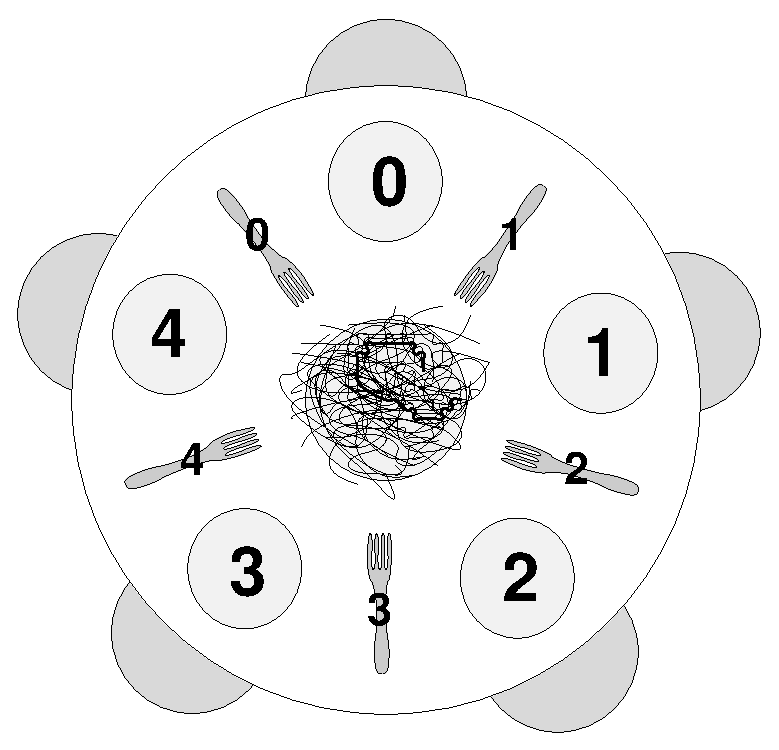
\includegraphics[height=2in]{table.eps}}

    با فرض اینکه چگونگی {\tt think} و {\tt eat} فیلسوف‌ها را بدانیم، وظیفه ما این است که 
    نسخه‌ای از {\tt get\_forks} و {\tt put\_forks}   را بنویسیم تا شرایط زیر را برآورده سازد:

\begin{itemize}

\item 
    در یک زمان تنها یک فیلسوف بتواند یک چنگال را در اختیار داشته باشد. 

\item 
    امکان بروز بن‌بست وجود نداشته باشد. 

\item 
    یک فیلسوف نباید به واسطه انتظار برای به دست آوردن یک چنگال دچار قحطی شود. 

\item 
    این امکان وجود داشته باشد که بیش از یک فیلسوف بتوانند به صورت همزمان غذا خورند. 

\end{itemize}

    آخرین نیازمندی، بیان دیگری از این مطلب است که راه‌حل باید کارا باشد؛ به این معنی که باید حداکثر مقدار همروندی را ممکن سازد. 

    درباره اینکه {\tt eat} و {\tt think} چقدر طول می‌کشد هیچ فرضی  را در نظر نمی‌گیریم، بجز آنکه در نهایت، {\tt eat}  باید خاتمه یابد. 
    در غیر اینصورت، إعمال محدودیت سوّم ناممکن است---اگر یک فیلسوف یکی از چنگال‌ها را تا ابد نگه دارد، 
    هیچ چیز نمی‌تواند مانع قحطی همسایه‌ها شود. 
    

    برای اینکه ارجاع فیلسوف‌ها به چنگال‌هایشان را ساده نماییم می‌توانیم از توابع {\tt left} و {\tt right} استفاده کنیم. 

\begin{latin}
\begin{lstlisting}[title=\rl{کدام چنگال؟}]{}
def left(i): return i
def right(i): return (i + 1) % 5
\end{lstlisting}
\end{latin}

    اپراتور {\tt \%} زمانیکه مقدار به ۵ برسد آن را به ۰ بر می‌گرداند؛ {\tt (4 + 1) \% 5 = 0}.

    از آنجایی که لازم است دسترسی انحصاری به چنگال‌ها را فراهم آوریم، طبیعی است که از لیستی از سمافورها استفاده کنیم، هر کدام برای یک چنگال. 
    در ابتدا تمامی چنگال‌ها موجودند. 

\begin{latin}
\begin{lstlisting}[title=\rl{متغیرهای غذا خوردن فیلسوف‌ها}]{}
forks = [Semaphore(1) for i in range(5)]
\end{lstlisting}
\end{latin}

    این نماد برای مقداردهی اولیه یک لیست ممکن است برای خوانندگانی که  پایتون را به کار نبرده‌اند ناآشنا باشد. 
    تابع {\tt range}، لیستی با پنج عنصر بر‌ می‌گرداند؛ برای هر عنصر این لیست، پایتون یک سمافور با مقدار اولیه ۱ ساخته 
    و نتیجه را در یک لیست به نام  {\tt forks} گرد می‌آورد.  

    تلاشی ابتدایی برای  {\tt get\_fork} و {\tt put\_fork} در ادامه آمده است:

\begin{latin}
\begin{lstlisting}[title=\rl{ناراه‌حل غذا خوردن فیلسوف‌ها}]{}
def get_forks(i):
    fork[right(i)].wait()
    fork[left(i)].wait()

def put_forks(i):
    fork[right(i)].signal()
    fork[left(i)].signal()
\end{lstlisting}
\end{latin}

    واضح است که این راه‌حل اوّلین شرط را برآورده می‌نماید، امّا می‌توانیم کاملاً مطمئن باشیم که دو شرط  بعدی برآورده نمی‌شود، زیرا که 
    اگر چنین بود، اصلاً مسأله جذابی نبوده و شما می‌توانستید به مطالعه فصل~\ref{next} بپردازید. 

    معمّا:‌ مشکل کجاست؟


\clearemptydoublepage
\subsection{بن‌بست \#5}

    اشکال کار در این است که میز گرد است. در نتیجه، هر فیلسوف می‌تواند یک چنگال را بر گرفته 
    و سپس برای همیشه منتظر چنگال دیگر بماند. بن‌بست! 

    معمّا: راه حلی برای این مسأله ارائه دهید که از بن‌بست جلوگیری نماید. 

    راهنمایی: یک راه اجتناب از بن‌بست این است که شرایطی که بن‌بست را ممکن می‌سازند را در نظر گرفته  و سپس یکی از آن‌ها را تغییر دهیم. 
    در این مساله، بن‌بست خیلی شکننده است--یک تغییر خیلی کوچک آن را در هم می‌شکند. 

\clearemptydoublepage
\subsection{راهنمایی غذا خوردن فیلسوف‌ها \#1}

    اگر تنها چهار فیلسوف در یک زمان مجاز به نشستن سر میز باشند، بن‌بست غیر ممکن می‌گردد. 

    ابتدا، خودتان را متقاعد نمایید که این ادّعا درست است، سپس کدی بنویسید که تعداد فیلسوف‌ها را سر میز محدود نمایید. 

%%  Wed 15 Jan 2020 06:02:19 PM +0330 : revision3

\clearemptydoublepage
\subsection{راه حل غذا خوردن فیلسوف‌ها  \#1}

    اگر تنها چهار فیلسوف سر میز باشند، آنگاه در بدترین حالت هر کدام یک چنگال را بر می‌دارد. سپس، تنها یک چنگال روی میز باقی‌ مانده و 
    آن چنگال دو همسایه دارد که هر کدام یک چنگال دیگر در دست دارند. بنابراین، هر کدام از همسایه‌ها می‌توانند چنگال باقی‌مانده را برداشته و غذا بخورد. 

    تعداد فیلسوف‌های سر میز را می‌توانیم با مالتی‌پلکسی با نام {\tt footman} که مقدار اولیه ۴ دارد کنترل کنیم. 
    راه‌حل مشابه زیر است: 

\begin{latin}
\begin{lstlisting}[title=\rl{راه حل غذا خوردن فیلسوف‌ها \#1}]{}
def get_forks(i):
    footman.wait()
    fork[right(i)].wait()
    fork[left(i)].wait()

def put_forks(i):
    fork[right(i)].signal()
    fork[left(i)].signal()
    footman.signal()
\end{lstlisting}
\end{latin}

    این راه‌حل علاوه بر اجتناب از بن‌بست،  تضمین می‌نماید که هیچ فیلسوفی دچار قحطی نشود. 
    تصور کنید که شما سر میز نشسته‌اید و هر دو همسایه شما مشغول غذا خوردن هستند. 
    شما در انتظار برای چنگال سمت راست، مسدوده شده‌اید. در نهایت همسایهٔ سمت راست شما، 
    چنگال را زمین خواهد گذاشت چرا که  {\tt eat} 
    نمی‌تواند تا ابد ادامه داشته باشد. از آنجاییکه شما تنها نخی هستید که منتظر آن چنگال هستید، لزوماً پس از آن، 
    چنگال را به دست خواهید آورد. 
    با استدلالی مشابه، در انتظار برای چنگال سمت چپ‌تان نیز دچار قحطی نخواهید شد. 
    
    بنابراین، زمانیکه یک فیلسوف می‌تواند سر میز بگذراند محدود است. همچنین این نکته دلالت بر این دارد که زمان انتظار برای ورود به اتاق 
    تا زمانیکه {\tt footman}  خصوصیت شمارهٔ ۴ را دارد، محدود است (بخش ~\ref{props} را ببینید). 
     
    

    این راه‌حل نشان می‌دهد که با کنترل کردن تعداد فیلسوف‌ها، می‌توانیم از بن‌بست اجتناب نماییم. 
    راه دیگر برای اجتناب از بن‌بست تغییر دادن ترتیبی است  که فیلسوف‌ها چنگال‌ها را بر می‌دارند. 
    در ناراه‌حل اولیه، فیلسوف‌ها "راست‌دست``\LTRfootnote{rightie} هستند؛ به این معنی که ابتدا چنگال سمت راست را بر می‌دارند. 
    امّا اگر فیلسوف ۰ "چپ‌دست``\LTRfootnote{leftie} باشد چه اتفاقی می‌افتد؟‌

    معمّا: ثابت کنید که اگر حداقل یکی از فیلسوف‌ها چپ‌دست و حداقل یکی راست‌دست باشد، آنگاه بن‌بست غیر ممکن است. 

    راهنمایی: بن‌بست تنها زمانی رخ می‌دهد که ۵ فیلسوف یک چنگال را در دست داشته و تا ابد منتظر چنگال دیگر می‌مانند. 
    در غیر اینصورت، یکی از آن‌ها می‌تواند هر دو چنگال را برداشته، غذا خورده و خارج شود. 

    اثبات با برهان خلف است.  ابتدا، تصور کنید که بن‌بست ممکن باشد. 
    سپس یکی از فیلسوف‌هایی که در بن‌بست گیر کرده است انتخاب نمایید. 
    اگر آن فیلسوف چپ‌دست باشد،‌ می‌توانید ثابت نمایید که تمامی‌ فیلسوف‌ها چپ‌دست هستند، که این خود یک تناقض است. 
    به طور مشابه، اگر راست‌دست باشد می‌توانید ثابت نمایید که همگی راست‌دست هستند. از هر دو طریق به تناقض می‌رسید؛ بنابراین 
    بن‌بست ممکن نیست. 
    
%%%%    Sat 11 Nov 2017 06:20:18 PM +0330

\clearemptydoublepage
\subsection{راه‌حل غذاخوردن فیلسوف‌ها \#2}

    در راه‌حل نامتقارن مسأله غذاخوردن فلیسوف‌ها، لازم است حداقل یک چپ دست و  حداقل یک راست دست سر میز باشند. 
    در این حالت، بن‌بست غیر ممکن است. راهنمایی قبل، طرح کلی اثبات را بیان می‌کند.
    در ادامه، جزئیات آمده است. 

    دوباره، اگر بن‌بست ممکن باشد، زمانی رخ می‌دهد که تمامی ۵ فیلسوف یک چنگال را نگاه داشته و منتظر چنگال دیگر بمانند. 
    اگر فرض کنیم فیلسوف $j$ چپ دست باشد آنگاه او باید چنگال سمت چپ را نگاه داشته و منتظر چنگال سمت راست باشد. 
    بنابراین همسایه سمت راست او (فیلسوف $k$) باید چنگال سمت چپش را نگاه داشته و منتظر همسایه راست خود باشد؛ به عبارت دیگر 
    فیلسوف $k$ باید چپ دست باشد. 
    با تکرار استدلال مشابه می‌توانیم ثابت کنیم که تمامی فیلسوف‌ها چپ دست هستند که با حکم اولیه که در آن 
    حداقل یک راست دست وجود دارد در تناقض است. لذا بن‌بست ممکن نیست. 

    استدلالی مشابه آنچه برای راه‌حل قبل به کار بردیم ثابت می‌کند که قحطی نیز غیر ممکن است. 


\clearemptydoublepage
\subsection{راه‌حل تننبام}

    در راه‌حل قبل هیچ چیز نادرستی وجود ندارد امّا تنها برای تکمیل بحث، بگذارید نگاهی به برخی راه حل‌های جایگزین بیندازیم. 
    یکی از شناخته‌ شده ترینِ  این راه حل‌ها، همانی است که در کتاب معروف سیستم‌عامل تننبام آمده است\cite{tanenbaum}. 
    برای هر فیلسوف یک متغیر وضعیت وجود دارد که نشان می‌دهد فیلسوف در کدامیک از حالات تفکر، 
    خوردن و یا در انتظار برای خوردن (''گرسنگی``) است و 
    یک سمافور که نشان می‌دهد آیا فیلسوف می‌تواند غذا خوردن را آغاز نماید نیز وجود دارد. 

\begin{latin}
\begin{lstlisting}[title=\rl{متغیرهای راه‌حل تننبام}]{}
state = ['thinking'] * 5
sem = [Semaphore(0) for i in range(5)]
mutex = Semaphore(1)
\end{lstlisting}
\end{latin}

    مقدار اولیه {\tt state} یک لیست ۵ تایی از {\tt 'thinking'} است.     {\tt sem}
    یک لیست ۵ تایی از سمافورهایی است با مقدار اولیه ۰. 
    و امّا کد: 

\begin{latin}
\begin{lstlisting}[title=\rl{ راه‌حل تننبام}]{}
def get_fork(i):
    mutex.wait()
    state[i] = 'hungry'
    test(i)
    mutex.signal()
    sem[i].wait()

def put_fork(i):
    mutex.wait()
    state[i] = 'thinking'
    test(right(i))
    test(left(i))
    mutex.signal()

def test(i):
    if state[i] == 'hungry' and
    state[left (i)]  != 'eating' and
    state[right (i)] != 'eating':
        state[i] = 'eating'
        sem[i].signal()
\end{lstlisting}
\end{latin}

% NOTE: need to fix this; see email from David Furcy.

    تابع {\tt test}  بررسی می‌کند که آیا فیلسوف $i$ام می‌تواند شروع به غذا خوردن نماید، و این در صورتی است که 
    او گرسنه بوده و هیچکدام از همسایه‌هایش در حال غذا خوردن نباشند. اگر چنین باشد، {\tt test} به سمافور $i$ سیگنال می‌دهد. 
    
    دو راه وجود دارد که یک فیلسوف می‌تواند غذا بخورد. در حالت اول، فیلسوف {\tt get\_forks} را اجرا کرده، 
    چنگال‌های موجود را یافته و 
    بلافاصله مشغول خوردن می‌شود. در حالت دوم، یکی از همسایه‌ها در حال غذا خوردن است 
    و فیلسوف روی سمافور خودش مسدود گردیده است. 
    نهایتاً یکی از همسایه‌ها دست از غذا می‌کشد و در این زمان  {\tt test} را روی هر دو همسایه خود اجرا می‌نماید. 
    ممکن است که هر دو بررسی موفقیت آمیز باشد، و در این حالت همسایه‌ها می‌توانند به صورت همروند مشغول غذا خوردن شوند. 
    ترتیب این دو بررسی اهمیتی ندارد. 

    یک نخ برای دسترسی به {\tt state} یا فراخوانی {\tt test}، باید {\tt mutex} را بگیرد. 
    بنابراین، عمل بررسی و به‌روزرسانی آرایه، اتمی است. از آنجایی که یک فیلسوف تنها زمانی می‌تواند 
    مشغول خوردن شود که بدانیم هر دو چنگال موجود است، 
    دسترسی انحصاری به چنگال‌ها تضمین شده است. 

    هیچ بن‌بستی ممکن نیست، زیرا تنها سمافوری که بیش از یک فیلسوف به آن دسترسی دارد، {\tt mutex} است و هیچ نخی  
    تا زمانی که {\tt mutex} را در اختیار دارد {\tt wait} را اجرا نمی‌نماید. 

%But again, starvation is tricky.
    امّا دومرتبه، قحطیْ ممکن ولی در اینجا خیلی مستلزم دقّت و مهارت است.

    معمّا: یا خودتان را متقاعد نمایید راه‌حل تننبام از قحطی جلوگیری می‌نماید و یا یک الگوی تکرارشونده بیابید که در آن، 
    یک نخ دچار قحطی شود در حالیکه مابقی نخ‌ها به کار خود ادامه می‌دهند. 


\clearemptydoublepage
\subsection{قحطی تننبام}

    متاسفانه، این راه‌حل مصون از قحطی نیست. \lr{Gingras} نشان داد الگوهای تکرارشونده‌ای وجود دارد که 
    در آن یک نخ برای همیشه منتظر مانده در حالیکه دیگر نخ‌ها می‌آیند و می‌روند\cite{gingras90dining}.

    تصور کنید که می‌خواهیم فیلسوف ۰ دچار قحطی شود. در ابتدا، ۲ و ۴ سر میز هستند و ۱ و ۳ گرسنه هستند. 
    تصور کنید که ۲ بر می‌خیزد و یک سر میز می‌نشیند؛ 
    سپس ۴ برخواسته و ۳ می‌نشیند. اکنون در وضعیتی مشابه موقعیت شروع هستیم. 

    اگر ۳ برخیزد و ۴ بنشیند، و سپس  برخواسته و ۲ بنشیند، به نقطه شروع بازگشته‌ایم. 
    این  حلقه را می‌توانیم تا ابد تکرار نماییم و در این صورت فیلسوف ۰ دچار قحطی می‌شود. 

    لذا راه‌حل تننبام تمامی ملزومات را برآورده نمی‌نماید. 


\clearemptydoublepage
\section {مسأله سیگاری‌ها}

    مسأله سیگاری‌ها در ابتدا توسط     \lr{Suhas Patil} مطرح شد \cite{patil}، و ادّعا نمود که  این مسأله با سمافورها قابل حل نیست. 
    این ادعا با تعدادی شرط همراه است، امّا در هر حالت مسأله جذاب و چالش برانگیز است. 

    چهار نخ در مسأله وجود دارد: یک عامل\LTRfootnote{agent} و سه سیگاری. 
    سیگاری‌ها تا ابد، در حلقهٔ ''ابتدا انتظار برای مواد مورد نیاز`` 
    و ''سپس ساختن`` و ''کشیدن سیگار`` هستند.
    مواد مورد نیاز شامل تنباکو، کاغذ و کبریت است. 

    فرض می‌کنیم که عامل، یک منبع لایزال از هر سه مادهٔ لازمه (کبریت، کاغذ و تنباکو) را  دارد 
    و هر سیگاری یک منبع نامتناهی از یکی از این سه مادهٔ لازمه را دارد، 
    بدین معنی که یکی از سیگاری‌ها کبریت، دیگری کاغذ و سومی نیز تنباکو دارد. 

    عامل، مکراراً دو ماده متفاوت را به صورت تصادفی انتخاب نموده و آن‌ها را به سیگاری‌ها عرضه می‌کند. 
    بسته به اینکه چه موادی انتخاب شده باشد، فرد سیگاری با ماده مکمل خود می‌تواند دو منبع را برداشته و ادامه دهد. 

    برای مثال اگر عامل، تنباکو و کاغذ بر دارد، فرد سیگاری که کبریت دارد می‌تواند هر دو ماده را برداشته 
    و یک سیگار ساخته و سپس به عامل سیگنال دهد. 

    برای توضیح فرض قبل،‌    
    عاملْ نشانگر یک سیستم‌عامل است که منابع را تخصیص می‌دهد، و سیگاری‌ها نشانگر برنامه‌هایی هستند که به منابع نیاز دارند. 
    مسأله این است که اطمینان دهیم اگر منابعی موجود هستند 
    که می‌توانند برای ادامهٔ فعالیت برنامه‌های بیشتری تخصیص داده شوند آن برنامه‌ها باید بیدار شوند. 
    متقابلاً، می‌خواهیم از بیدار نمودن برنامه‌هایی که نمی‌توانند به کار خود ادامه دهند اجتناب نماییم. 


    طبق این فرض، سه نسخه از این مسأله وجود دارد که اغلب در کتاب‌ها مشاهده می‌شود: 

\begin{description}

\item
    [نسخهٔ غیرممکن:] نسخه \lr{Patil} محدودیت‌هایی روی راه‌حل تحمیل می‌نماید. اوّل اینکه، شما اجازهٔ تغییر کد عامل را ندارید. 
    اگر عامل نشانگر یک سیستم‌عامل باشد، این فرض که شما نمی‌خواهید کد سیستم عامل را هر زمان که یک برنامه جدید می‌آید تغییر دهید 
    بی معنی نیست. 
    محدودیت دوم این است که شما نمی‌توانید از عبارات شرطی یا یک آرایه‌ای از سمافورها استفاده نمایید. با این محدودیت‌ها، 
    مسأله قابل حل نیست، امّا همانطور که  \lr{Patil} اشاره نموده است محدودیت دوم کاملاً مصنوعی است  \cite{Parnas}. 
    با محدودیت‌هایی نظیر این دو، مسائل بسیاری غیر قابل حل خواهد شد. 

\item
    [نسخهٔ جذّاب:] این نسخه محدودیت اول (عدم امکان تغییر کد عامل) را دارد ولی مابقی را در نظر نمی‌گیرد.
    
\item
%to the ingredients that are available.  This version of the problem
%is uninteresting because it makes the whole premise, the ingredients
%and the cigarettes, irrelevant.  Also, as a practical matter, it is
    [نسخهٔ بدیهی:] در برخی کتاب‌ها، در خود مسأله آمده است که عامل باید بر مبنای مواد موجود به آن فرد سیگاری که 
    می‌تواند ادامه دهد سیگنال ارسال نماید. 
    این نسخه از مسأله، جذّابیتی ندارد زیرا که تمام فرض اوّلیه --مواد لازمه و سیگارها-- را بی‌ربط می‌سازد. همچنین در عمل، احتمالاً     
     اینکه عامل، اطلاعی از سایر نخ‌ها و آنچه که آن‌ها نیاز دارند داشته باشد ایده خوبی نیست. 
     در نهایت،  این نسخه از مسأله نیز بسیار ساده است.
     
\end{description}
%%%%        Sat 18 Nov 2017 06:11:58 PM +0330
%%%        Tue 28 Jan 2020 05:58:30 PM +0330; revision3

    طبیعتاً روی نسخه جذّاب تمرکز می‌نمایم. برای تکمیل بیان مسأله، باید کد عامل را مشخص نماییم. عامل، سمافورهای زیر را بکار می‌برد:

\begin{latin}
%\begin{lstlisting}[title={Agent semaphores}]{}
\begin{lstlisting}[title=\rl{سمافورهای عامل}]{}
agentSem = Semaphore(1)
tobacco = Semaphore(0)
paper = Semaphore(0)
match = Semaphore(0)
\end{lstlisting}
\end{latin}

    عامل در واقع از سه نخ همروند تشکیل شده است:  عامل \lr{A}،  عامل \lr{B} و عامل \lr{C}.
    هر کدام از آن‌ها روی {\tt agentSem} منتظر می‌مانند؛ هر گاه که {\tt agentSem} سیگنالی دریافت کند، یکی از عامل‌ها بر می‌خیزد و 
    از طریق سیگنال‌دهی به دو سمافور، مواد مورد نیاز را فراهم می‌آورد. 

\begin{latin}
\begin{lstlisting}[title=\rl{کد عامل \lr{A}}]{}
agentSem.wait()
tobacco.signal()
paper.signal()
\end{lstlisting}
\end{latin}


\begin{latin}
\begin{lstlisting}[title=\rl{کد عامل \lr{B}}]{}
agentSem.wait()
paper.signal()
match.signal()
\end{lstlisting}
\end{latin}

\begin{latin}
\begin{lstlisting}[title=\rl{کد عامل \lr{C}}]{}
agentSem.wait()
tobacco.signal()
match.signal()
\end{lstlisting}
\end{latin}

%work.  It is tempting to write something like:
    این مسأله آنقدرها هم ساده نیست زیرا که راه‌حل طبیعی آن کار نمی‌کند.  ممکن است وسوسه شوید تا کدی مانند زیر بنویسید:
%    نوشتن کدی مانند زیر، وسوسه انگیز است: 
    

\begin{latin}
%\begin{lstlisting}[title={Smoker with matches}]{}
\begin{lstlisting}[title=\rl{‌سیگاری کبریت‌دار}]{}
tobacco.wait()
paper.wait()
agentSem.signal()
\end{lstlisting}
\end{latin}

\begin{latin}
%\begin{lstlisting}[title={Smoker with tobacco}]{}
\begin{lstlisting}[title=\rl{سیگاری تنباکو‌دار}]{}
paper.wait()
match.wait()
agentSem.signal()
\end{lstlisting}
\end{latin}

\begin{latin}
%\begin{lstlisting}[title={Smoker with paper}]{}
\begin{lstlisting}[title=\rl{سیگاری کاغذدار}]{}
tobacco.wait()
match.wait()
agentSem.signal()
\end{lstlisting}
\end{latin}

    مشکل این  راه‌حل کجاست؟

\clearemptydoublepage
\subsection{بن‌بست \#6}

    مشکل راه‌حل قبل امکان وقوع بن‌بست است. تصور کنید که عامل، تنباکو و کاغذ عرضه می‌نماید. از آنجایی که فرد  سیگاری‌ که در دست خود کبریت دارد 
    منتظر {\tt tobacco} ممکن است رفع انسداد گردد. امّا آن فرد سیگاری که در دست خود تنباکو دارد منتظر {\tt paper} است، لذا ممکن است او نیز 
    رفع انسداد گردد (احتمال آن نیز زیاد است). سپس اوّلین نخ روی {\tt paper} مسدود گردیده و دومی نیز روی {\tt match} مسدود می‌گردد و بن‌بست!. 

\clearemptydoublepage
\subsection{راهنمایی مسأله سیگاری‌ها}

    راه‌حل \lr{Parnas}، 
    سه نخ کمکی را  تحت عنوان "فروشندگان غیر مجاز``\LTRfootnote{pusher} به کار می‌برد که آن‌ها به سیگنال‌هایی که از عامل‌
    می‌رسد پاسخ داده، میزان موجودی مواد مورد نیاز را نگاه داشته و به فرد سیگاری مناسب سیگنال می‌دهند. 

    متغیرها و سمافورهای اضافی به شرح زیر است: 

\begin{latin}
\begin{lstlisting}[title=\rl{راهنمایی مسأله سیگاری‌ها}]{}
isTobacco = isPaper = isMatch = False
tobaccoSem = Semaphore(0)
paperSem = Semaphore(0)
matchSem = Semaphore(0)
\end{lstlisting}
\end{latin}

    متغیرهای بولی نشان می‌دهند که آیا یک مادهٔ مورد نیاز، وجود دارد یا خیر. 
    فروشنده‌‌ها از {\tt tobaccoSem} استفاده نموده تا به آن فرد سیگاری که تنباکو در دست دارد سیگنال دهند و سمافورهای دیگر نیز به همین شیوه به کار می‌روند.


\clearemptydoublepage
\subsection{راه حل مسأله سیگاری}

    کد یکی از فروشندگان در ادامه آمده است:‌

\begin{latin}
%\begin{lstlisting}[title={Pusher A}]{}
\begin{lstlisting}[title=\rl{فروشنده \lr{A}}]{}
tobacco.wait()
mutex.wait()
    if isPaper:
        isPaper = False
        matchSem.signal()
    elif isMatch:
        isMatch = False
        paperSem.signal()
    else: 
        isTobacco = True
mutex.signal()
\end{lstlisting}
\end{latin}

    این فروشنده هر زمان که تنباکو موجود باشد فعال می‌شود. اگر مقدار {\tt isPaper} برابر \lr{True} باشد، می‌داند که فروشندهٔ‌ \lr{B} نیز در حال 
    حاضر فعال است، لذا می‌تواند به آن فرد سیگاری که در دست خود کبریت دارد سیگنال دهد. به طور مشابه، اگر کبریت موجود باشد می‌تواند به آن فرد 
    سیگاری که در دست خود کاغذ دارد سیگنال دهد. 

    امّا اگر نخست فروشنده \lr{A} اجرا شود، سپس هر دوی {\tt isPaper} و  {\tt isMatch}  را \lr{False} می‌بیند و نمی‌تواند به هیچ‌کدام از افراد 
    سیگاری سیگنال دهد لذا مقدار  {\tt isTobacco} را \lr{True}  می‌نماید. 

    فروشنده‌های دیگر نیز چنین هستند. از آنجایی که  تمام کار اصلی را فروشنده‌ها انجام می‌دهند، کد سیگاری بدیهی می‌شود.

\begin{latin}
%\begin{lstlisting}[title={Smoker with tobacco}]{}
\begin{lstlisting}[title=\rl{سیگاری تنباکو‌دار}]{}
tobaccoSem.wait()
makeCigarette()
agentSem.signal()
smoke()
\end{lstlisting}
\end{latin}

    \lr{Parnas}
    راه‌حل مشابهی ارائه می‌دهد که متغیرهای بولی را به صورت بیتی در یک متغیر صحیح ذخیره نموده است و سپس عدد صحیح را به عنوان 
    اندیس آرایه‌ای از سمافورها بکار می‌برد. با این شیوه، راه‌حل او از بکاربردن عبارات شرطی اجتناب می‌نماید (یکی از محدودیت‌های ساختگی، عدم استفاده 
    از عبارات شرطی و آرایه‌ای از سمافورها بود). 
    کد حاصل کمی خلاصه‌تر است، امّا عملکردش آنقدر واضح نیست. 
    
%%%    Sun 26 Nov 2017 05:59:38 PM +0330

\subsection{ مسألهٔ تعمیم یافتهٔ سیگاری‌ها}

    \lr{Parnas}
     پیشنهاد نمود که اگر عامل را به این صورت دستکاری کنیم
     که نیازی نباشد تا عامل پس از گذاشتن مواد لازم صبر نماید، آنگاه مسأله سیگاری‌ها دشوارتر خواهد شد. 
    در این حالت، باید چند نمونه از یک مادهٔ لازم روی میز موجود باشد. 

    معمّا: راه‌حل قبل را به گونه‌ای دستکاری کنید که با این تغییر مطابقت داشته باشد. 

\clearemptydoublepage
\subsection{راهنمای مسألهٔ تعمیم یافتهٔ سیگاری‌ها}

    اگر عامل، منتظر سیگاری‌ها نماند، ممکن است موارد لازم روی میز انباشته شود. بجای استفاده از مقادیر بولی به منظور ردگیری موارد لازم، 
    به مقادیر صحیح برای شمارش آن‌ها نیاز داریم. 

\begin{latin}
\begin{lstlisting}[title=\rl{راهنمای  مسألهٔ تعمیم یافتهٔ سیگاری‌ها}]
numTobacco = numPaper = numMatch = 0
\end{lstlisting}
\end{latin}


\clearemptydoublepage
\subsection{راه‌حل مسألهٔ تعمیم یافتهٔ سیگاری‌ها}
\label{smoker}

    کد تغییر یافتهٔ فروشندهٔ \lr{A} در ادامه آمده است: 

\begin{latin}
\begin{lstlisting}[title={\rl{فروشنده} A}]{}
tobacco.wait()
mutex.wait()
    if numPaper:
        numPaper -= 1
        matchSem.signal()
    elif numMatch:
        numMatch -= 1
        paperSem.signal()
    else: 
        numTobacco += 1
mutex.signal()
\end{lstlisting}
\end{latin}

    یک راه تصویرسازی این مسأله این است که تصوّر نمایید آنزمان که عاملی اجرا می‌شود‌، دو فروشنده را ایجاد نموده و به هر کدام از آن‌ها یکی از مواد لازم را 
    می‌دهد و آن‌ها را همراه با سایر فروشندگان در یک اتاق قرار می‌دهد. به خاطر وجود میوتکس، فروشنده‌ها در اتاقی که سه سیگاری خوابیده و یک میز وجود دارد 
    به ترتیب وارد می‌شوند. هر فروشنده یکی پس از دیگری وارد اتاق شده و مواد روی میز را بررسی می‌نماید. اگر او بتواند یک مجموعه کامل از مواد لازم سیگار را
    گرد آورد، آن‌ها از روی میز برداشته و سیگاری متناظر را بیدار می‌نماید. و اگر نتواند،‌ مواد همراه خود را روی میز رها کرده و اتاق را بدون اینکه کسی را 
    بیدار کند ترک می‌نماید. 

    این مثالی از الگویی است که آن را «جدول امتیاز»\LTRfootnote{scoreboard} خوانده و بعداً چندین مرتبه آن را خواهیم دید.   
    متغیرهای     {\tt numPaper}، {\tt numTobacco} و  {\tt numMatch}    وضعیت سیستم را نگاه می‌دارند. 
    از آنجایی که هر نخ از طریق میوتکس به ترتیب وارد می‌شود، مثل اینکه به جدول امتیاز نگاه کرده باشد وضعیت را بررسی نموده و مطابق آن عکس العمل نشان می‌دهد. 


%%%    Tue 04 Feb 2020 06:02:50 PM +0330 revision3

\clearemptydoublepage
\chapter{مسائل همگام‌سازی کمتر-کلاسیک}
\label{next}


\section{مسأله غذاخوردن وحشی‌ها}

    این مسأله از  \emph{برنامه‌نویسی همروند} \lr{Andrews}  اقتباس شده است\cite{andrews}. 

\begin {quotation}
    قبیله‌ای از وحشی‌ها، از یک دیگ بزرگ که می‌تواند \lr{M}  
    پرس از کشیش پخته شده را در خود نگاه دارد به صورت مشترک شام می‌خورند.\footnote{%
    این مسأله بر پایهٔ تصویری کارتونی از تاریخ مبلغین غربی در میان جوامع تشکیل شده با محوریت شکار است. 
    تعمداً مقداری طنز با کنایه به مسأله غذاخوردن فلیسوف‌ها به کار رفته است 
    امّا در اینجا تصویر وحشی‌ها واقع‌بینانه‌تر از تصویر قبلی از فیلسوف‌ها نیست. 
    اگر به جوامع شکار-محور علاقه‌مند هستید می‌توانید منابع زیر را مطالعه کنید:
    \lr{\em Guns,Germs and Steel} از \lr{Jared Diamond}،
    \lr{\em The Yanomamo} از \lr{Napoleon Chagnon} و یا 
    \lr{\em In Trouble Again} از \lr{Redmond O'Hanlon}.
    البته \lr{\em Darkness in El Dorado} از \lr{Tierney} را اکیداً توصیه نمی‌کنم زیرا که به نظرم غیر واقعی است.}
    زمانیکه یک وحشی می‌خواهد غذا بخورد، از درون دیگ از خود پذیرایی می‌کند مگر اینکه دیگ خالی باشد. 
    اگر دیگ خالی بود، وحشی آشپز را بیدار نموده و سپس منتظر او می‌ماند تا دومرتبه دیگ را پر نماید.
\end{quotation}

    هر تعداد از نخ‌های وحشی می‌تواند کد زیر را اجرا نماید:

\begin{latin}
\begin{lstlisting}[title=\rl{کد ناهمگام یک وحشی}]{}
while True:
    getServingFromPot()
    eat()
\end{lstlisting}
\end{latin}

    و نخ یک آشپز کد زیر را اجرا می‌نماید:

\begin{latin}
\begin{lstlisting}[title=\rl{کد ناهمگام آشپز}]{}
while True:
    putServingsInPot(M)
\end{lstlisting}
\end{latin}

    محدودیت‌های همگام‌سازی عبارتند از:

\begin{itemize}

\item 
    اگر دیگ خالی باشد وحشی‌ها نمی‌توانند {\tt getServingFromPot}  را فراخوانند. 

\item 
    آشپز تنها در صورتی می‌تواند  {\tt putServingsInPot} را فراخواند که دیگ خالی باشد. 

\end{itemize}

    معمّا: کدی برای وحشی‌ها و آشپز اضافه نمایید که محدودیت‌های همگام‌سازی را برآورده نماید. 
%%%Sat 02 Dec 2017 06:03:27 PM +0330

\clearemptydoublepage
\subsection{راهنمایی غذاخوردن وحشی‌ها}

    همانند مسأله تولیدکننده-مصرف‌کننده  در اینجا نیز وسوسه می‌شویم که برای نگهداری تعداد پرس‌ها از سمافور استفاده نماییم. 
    امّا به منظور سیگنال‌دهی به آشپز،‌ آن زمانی که دیگ خالی است، 
    یک نخ پیش از اینکه مقدار سمافور را کاهش دهد باید بداند که آیا باید منتظر بماند؟ و 
    ما نمی‌توانیم چنین کاری کنیم. 

    بکارگیری جدول امتیاز به منظور نگهداری تعداد پرس‌ها می‌تواند به عنوان گزینه‌ای دیگر مطرح شود.
    اگر یک وحشی شمارنده را صفر بیابد، آشپز را بیدار نموده و منتظر دریافت سیگنال پرشدن دیگ می‌شود. 
    متغیرهایی را که به کار برده‌ایم در ادامه مشاهده می‌نمایید:

\begin{latin}
\begin{lstlisting}[title={Dining Savages hint}]{}
servings = 0
mutex = Semaphore(1)
emptyPot = Semaphore(0)
fullPot = Semaphore(0)
\end{lstlisting}
\end{latin}

    {\tt emptyPot} نشانگر خالی بودن دیگ است و {\tt fullPot} بیانگر پربودن دیگ است. 

\clearemptydoublepage
\subsection{راه‌ حل غذاخوردن وحشی‌ها}

    راه‌حل،  ترکیبی از الگوی جدول امتیاز با یک قرار ملاقات است.  کد آشپز در ادامه آمده است. 

\begin{latin}
\begin{lstlisting}[title=\rl{راه‌‌حل غذاخوردن وحشی‌ها (آشپز)}]{}
while True:
    emptyPot.wait()
    putServingsInPot(M)
    fullPot.signal()
\end{lstlisting}
\end{latin}

    کد وحشی‌ها کمی پیچیده‌تر است. از آنجایی که هر وحشی از میوتکس می‌گذرد لذا دیگ را بررسی می‌نماید. 
    اگر دیگ خالی باشد، به آشپز سیگنال داده و منتظر می‌ماند و الّا  {\tt servings} را کاهش داده و پرسی را از دیگ بر می‌دارد. 

\begin{latin}
\begin{lstlisting}[title=\rl{راه‌‌حل غذاخوردن وحشی‌ها (وحشی)}]{}
while True:
    mutex.wait()
        if servings == 0:
            emptyPot.signal()
            fullPot.wait()
            servings = M
        servings -= 1
	getServingFromPot()
    mutex.signal()

    eat()
\end{lstlisting}
\end{latin}

    اینکه وحشی بجای آشپز دستور {\tt servings = M} را اجرا می‌کند شاید کمی عجیب بنظر آید. 
    واقعاً ضرورتی به اینکار نبود، زمانی که 
    آشپز {\tt putServingsInPot} را اجرا می‌نماید، می‌دانیم آن وحشی که میوتکس را در اختیار دارد 
    روی {\tt fullPot} منتظر می‌ماند. 
    لذا آشپز به  {\tt servings} دسترسی اَمنی دارد.  
    امّا در این حالت،‌ تصمیم گرفتم که وحشی این کار را انجام دهد چنانکه با نگاه به کد نیز 
    واضح است که تمامی دسترسی‌های به  {\tt servings} درون میوتکس انجام می‌پذیرد. 
    

    این راه حل، بدون بن‌بست است. 
    تنها شانس بن‌بست زمانی است که آن وحشی‌ای که {\tt mutex}  را نگاه داشته و منتظر {\tt fullPot} می‌ماند. 
    زمانیکه او منتظر است، سایر وحشی‌ها روی {\tt mutex} در صف انتظار قرار می‌گیرند. 
    امّا نهایتاً آشپز اجرا شده و به {\tt fullPot} سیگنال می‌دهد، 
    و این منجر به این می‌شود که  وحشی منتظر، ادامه یافته و میوتکس را آزاد نماید. 
    

    آیا این راه‌حل فرض نموده است که دیگ، نخ-ایمن\footnote{%
    در برنامه‌نویسی چند نخی، کدی را نخ-ایمن گوییم که تضمین نماید ساختمان داده‌های اشتراکی 
    بدون دخالت‌های ناخواسته دیگر نخ‌ها، به‌روزرسانی شود.%
    }  است و یا تضمین می‌نماید که  {\tt putServingsInPot} و {\tt getServingFromPot} 
    به صورت انحصاری انجام شوند؟


\clearemptydoublepage
\section{مسأله آرایشگاه}

ب    مسأله اصلی آرایشگر بوسیله \lr{Dijkstra} پیشنهاد شد. 
    یک گونهٔ دیگر آن در کتاب اصول سیستم‌های عامل \lr{Silberschatz} و \lr{Galvin}
    آمده است\cite{silberschatz}. 

\begin {quotation}
    یک آرایشگاه شامل $n$ صندلی در اتاق انتظار و یک صندلی آرایش در اتاق آرایشگر است. 
    اگر هیچ مشتری وجود نداشته باشد آرایشگر می‌خوابد. 
    اگر یک مشتری وارد آرایشگاه شود و تمامی صندلی‌ها اشغال شده باشد، آنگاه مشتری مغازه را ترک می‌نماید. 
    اگر آرایشگر مشغول باشد، امّا صندلی موجود باشد، مشتری روی یکی از صندلی‌های خالی می‌نشیند. 
    اگر آرایشگر خواب باشد، مشتری او را بیدار می‌نماید. 
    برنامه‌ای بنویسید که آرایشگر و مشتری‌ها را هماهنگ نماید. 
\end{quotation}

    برای اینکه مسأله را کمی واقعی‌تر نماییم، اطلاعات زیر را به آن می‌افزاییم: 

\begin{itemize}

\item
    نخ‌های مشتری باید تابعی به نام {\tt getHairCut} را فراخوانند. 

\item 
    اگر زمانیکه آرایشگاه پر است یک نخ مشتری برسد، می‌تواند {\tt balk} را که هیچ مقداری بر نمی‌گرداند،  فراخواند. 

\item 
    نخ آرایشگر باید {\tt cutHair} را فراخواند. 

\item 
    زمانیکه آرایشگر {\tt cutHair} را فرا می‌خواند،‌ 
    باید دقیقاً تنها یک نخ باشد که به طور همزمان  {\tt getHairCut} را فرا می‌خواند. 

\end{itemize}

    راه‌حلی ارائه دهید  که شرایط فوق را تضمین نماید. 


\clearemptydoublepage
\subsection{راهنمایی آرایشگاه}

\begin{latin}
\lstinputlisting[title=\rl{راهنمایی آرایشگاه}]{../code/barber.py.0}
\end{latin}

    {\tt n}    تعداد کل مشتری‌هایی است که می‌توانند در آرایشگاه باشند: سه نفر در اتاق انتظار و یک نفر روی صندلی آرایش. 

    {\tt customers}        تعداد مشتری‌های درون آرایشگاه را می‌شمرد و بوسیله  {\tt mutex} حفاظت می‌ شود. 
    

    آرایشگر روی {\tt customer} منتظر می‌ماند تا یک مشتری وارد شود، 
    سپس مشتری روی  {\tt barber} می‌ماند تا زمانیکه آرایشگر به او سیگنال نشستن روی صندلی آرایش را بدهد. 

    پس از آرایش مو، مشتری به  {\tt customerDone}  سیگنال می‌دهد و روی {\tt barberDone} منتظر می‌ماند. 

\clearemptydoublepage
\subsection{راه‌حل آرایشگاه}

    این راه‌حل یک جدول امتیاز و دو قرار ملاقات را ترکیب می‌نماید. کد مشتری‌ها در ادامه آمده است. 

\begin{latin}
\lstinputlisting[title=\rl{راه‌حل آرایشگاه (مشتری)}]{../code/barber.py.1}
\end{latin}

    اگر  $n$ مشتری در آرایشگاه وجود داشته باشد، هر مشتری که می‌رسد بلافاصله {\tt balk} را فرا می‌خواند 
    و الّا هر مشتری به {\tt customer} سینگال داده و روی {\tt barber} منتظر می‌ماند. 

    % typo: barbers -> barber
%Here is the code for barbers:
    کد آرایشگر در ادامه آمده است. 

\begin{latin}
\lstinputlisting[title=\rl{راه‌حل آرایشگاه (آرایشگر)}]{../code/barber.py.2}
\end{latin}

    هر زمان که  یک مشتری سیگنال می‌دهد، آرایشگر بیدار شده، به  {\tt barber} سیگنال می‌دهد، و مشغول آرایش یک نفر می‌شود. 
    اگر آن زمانیکه آرایشگر مشغول است مشتری دیگری برسد، 
    آنگاه در تکرار بعدی آرایشگر بدون اینکه بخوابد از سمافور {\tt customer} می‌گذرد. 

    اسامی {\tt customer} و {\tt barber} بر مبنای قرارداد نامگذاری یک قرار ملاقات هستند، لذا {\tt customer.wait()} 
    به معنای ''انتظار برای یک مشتری`` است و نه اینکه ''مشتری‌های در اینجا منتظرند``. 

    قرار ملاقات دوم با استفاده از  {\tt customerDone} و {\tt barberDone}، تضمین می‌نماید کار آرایش فعلی تمام شده باشد
    پیش از اینکه آرایشگر به ابتدای حلقه برگردد و به مشتری بعدی اجازه ورود به ناحیه بحرانی را بدهد. 

    این راه‌حل در \verb"sync_code/barber.py" آمده است (ر.ک.~\ref{sync.py}).
%%%    Mon 04 Dec 2017 06:21:40 PM +0330
%%% Tue 07 Apr 2020 06:36:26 PM +0430   revision: #3
\clearemptydoublepage
\section{آرایشگاه FIFO}

    در راه‌حل قبل تضمینی وجود ندارد که مشتریان به همان ترتیبی که می‌رسند سرویس دریافت کنند.
    تا سقف {\tt n} مشتری می‌توانند از ترن‌استایل گذر کنند، به {\tt customer} سیگنال داده، 
    و روی {\tt barber} منتظر بمانند. زمانیکه آرایشگر به {\tt barber} سیگنال دهد، هر یک از 
    مشتریان ممکن است ادامه دهد.

	این راه‌حل را به گونه‌ای تغییر دهید که مشتریان به همان ترتیبی که از ترن‌استایل عبور می‌کنند سرویس دریافت نمایند.
  
	راهنمایی: می‌توانید به نخ جاری به صورت {\tt self} ارجاع دهید، 
	لذا وقتی می‌نویسد {\tt self.sem = Semaphore(0)}، هر نخ سمافور خودش را می‌گیرد.


\clearemptydoublepage
\subsection{راهنمایی آرایشگاه FIFO}

	من از لیستی از سمافورها به نام {\tt queue} در راه‌حل خود استفاده می‌کنم.

\begin{latin}
\lstinputlisting[title=\rl{راهنمایی آرایشگاه \lr{FIFO}}]{../code/barber2.py.0}
\end{latin}

%%%%typo: a thread -> a semophore
%As each thread passes the turnstile, it creates a thread and puts it
%in the queue.
	زمانی‌که هر یک از نخ‌ها از ترن‌استایل عبور می‌کند، یک سمافور ساخته و آن را در صف قرار می‌دهد.

	به جای انتظار روی {\tt barber}، هر نخ روی سمافور خودش منتظر می‌ماند. 
	وقتیکه آرایشگر بیدار می‌شود، یک سمافور را از صف خارج کرده و به آن سیگنال می‌دهد.


\clearemptydoublepage
\subsection{راه‌حل آرایشگاه FIFO}

	در ادامه کد تغییریافتهٔ مشتریان آمده است:

\begin{latin}
\lstinputlisting[title=\rl{راه‌حل آرایشگاه \lr{FIFO} (مشتری)}]
{../code/barber2.py.1}
\end{latin}

	و کد آرایشگر به این صورت است:

\begin{latin}
\lstinputlisting[title=\rl{راه‌حل آرایشگاه \lr{FIFO} (آرایشگر)}]
{../code/barber2.py.2}
\end{latin}

	توجه نمایید که آرایشگر باید {\tt mutex} را بگیرد تا به صف دسترسی داشته باشد.

	این راه‌حل در \verb"sync_code/barber2.py" آمده است (ر.ک.~\ref{sync.py}).

\clearemptydoublepage
%\section {Hilzer's Barbershop problem}
\section {مسألهٔ آرایشگاه هیلزر}

	ویلیام استالینگز\LTRfootnote{William Stallings} \cite{stallings}  
	یک نسخهٔ پیچیده‌تر از مسألهٔ آرایشگاه را ارائه می‌دهد، 
	که آن را مدیون رالف هیلزر\LTRfootnote{Ralph Hilzer} در دانشگاه ایالتی کالیفرنیا در چیکو می‌داند.

\begin{quotation}
    آرایشگاه ما سه تا صندلی،‌ سه تا آرایشگر و اتاق انتظاری دارد که  چهار مشتری می‌توانند روی یک کاناپه قرار گیرند و مابقی بایستند. 
    طبق قوانین آتش‌نشانی تعداد کل مشتری‌های داخل آرایشگاه نباید از ۲۰ تا تجاوز نماید. 
    
    اگر ظرفیت داخل آرایشگاه تکمیل باشد، مشتری جدید وارد مغازه نخواهد شد. 
    زمانیکه مشتری داخل است اگر روی کاناپه جا باشد می‌نشیند در غیر اینصورت می‌ایستد. 
    زمانیکه یک آرایشگر آزاد باشد، آن مشتری که بیشترین زمان را روی کاناپه بوده  سرویس دریافت می‌کند و اگر مشتریان ایستاده وجود داشته باشند 
    آن فردی که مدت زمان بیشتری را در آرایشگاه بوده است جای او را روی کاناپه خواهد گرفت. 
    زمانیکه آرایش یک مشتری تمام شد،‌ هر آرایشگر می‌تواند اجرت را دریافت دارد،‌ امّا از آنجایی که تنها یک صندوق وجود دارد
    در هر زمان تنها یک مشتری می‌تواند پرداخت خود را انجام دهد. 
    آرایشگران زمان خود را اینچنین تقسیم می‌نمایند: آرایش، دریافت وجه و خوابیدن روی صندلی در حالیکه منتظر مشتری هستند.
\end{quotation}

    به عبارت دیگر، محدودیت‌های همگام‌سازی زیر اعمال می‌شود:

\begin{itemize}

\item 
    مشتریان توابع زیر را به ترتیب فرا می‌خوانند:
{\tt enterShop}, {\tt sitOnSofa},
{\tt getHairCut}, {\tt pay}.   
%%typo: ,and for the last one. 

\item 
    آرایشگران  {\tt cutHair} و {\tt acceptPayment} را فرا می‌خوانند. 

\item 
     اگر ظرفیت آرایشگاه پر باشد مشتریان نمی‌توانند {\tt enterShop}  را فراخوانی نمایند. 

\item 
    اگر کاناپه پر باشد، مشتری‌ تازه وارد نمی‌تواند {\tt sitOnSofa} را فراخواند. 

\item 
    زمانیکه یک مشتری {\tt getHairCut} را فرا می‌خواند متناظراً  یک آرایشگر باید {\tt cutHair} را به صورت همزمان اجرا نماید و بالعکس. 

\item 
    فراخوانی {\tt getHairCut} به صورت همزمان حداکثر توسط سه مشتری  و اجرای {\tt cutHair} به طور همزمان توسط حداکثر 
    سه آرایشگر  ممکن باشد.

\item 
    مشتری باید قبل از اینکه آرایشگر بتواند {\tt acceptPayment} را فراخواند،  {\tt pay}  را اجرا نماید. 

\item 
    آرایشگر می‌بایست  {\tt acceptPayment} را قبل از خروج مشتری  اجرا نماید. 

\end{itemize}

    معمّا: کدی بنویسید که محدودیت‌های همگام‌سازی آرایشگاه هیلزر را اعمال نماید. 


\subsection{راهنمایی آرایشگاه هیلزر}

    متغیرهایی که در راه‌حل بکار رفته در ادامه آمده است:‌

\begin{latin}
\lstinputlisting[title=\rl{راهنمایی آرایشگاه هیلزر}]
{../code/barber3.py.0}
\end{latin}

    {\tt mutex}
    از {\tt customers} که تعداد مشتری‌های درون آرایشگاه را در خود دارد و  از {\tt queue1} که لیست سمافورهای نخ‌های منتظر برای نشستن 
    روی کاناپه است حفاظت می‌نماید. 	

%{\tt mutex2} protects {\tt queue2}, which is a list
%of semaphores for threads waiting for a chair.
    {\tt mutex2} 
    از {\tt queue2} (یک لیست از سمافورهای نخ‌های در انتظار صندلی) حفاظت می‌کند. 

    {\tt sofa} 
    یک مالتی‌پلکس است که حداکثر تعداد مشتری‌های روی کاناپه را کنترل می‌کند.

    {\tt customer1}
    پیغام می‌دهد که یک مشتری در  {\tt queue1} وجود دارد و {\tt customer2} پیغام می‌دهد که یک مشتری در  {\tt queue2} وجود دارد. 

     {\tt payment}
    پیغام می‌دهد که یک مشتری پرداخت داشته است و {\tt receipt} پیغام می‌دهد که آرایشگر اجرت را دریافت کرده است. 


\clearemptydoublepage
\subsection {راه‌حل آرایشگاه هیلزر}

    این راه‌حل به طور قابل توجهی از آنچه انتظار داشتم پیچیده‌تر است. شاید در ذهن هیلزر راه‌حل ساده‌تری وجود داشته است لکن 
    این بهترین چیزی است که می‌توانستم ارائه دهم. 

\begin{latin}
\lstinputlisting[title=\rl{راه‌حل آرایشگاه هیلزر (مشتری)}]
{../code/barber3.py.1}
\end{latin}

    اوّلین پاراگراف مشابه راه‌حل قبلی است. زمانیکه یک مشتری می‌رسد، شمارنده را بررسی نموده آنگاه یا از ورود امتناع ورزیده و یا خودش را به 
    صف می‌افزاید. سپس به آرایشگر سیگنال می‌دهد. 

    زمانیکه مشتری از صف خارج می‌شود، وارد مالتی‌پلکس می‌گردد، روی مبل می‌نشیند و خود را به صف دوم می‌افزاید. 

    زمانیکه از \textbf{آن} صف خارج می‌شود، آرایش شده، پرداخت انجام داده و خارج می‌شود.

\begin{latin}
\lstinputlisting[title=\rl{راه‌حل آرایشگاه هیلزر (آرایشگر)}]
{../code/barber3.py.2}
\end{latin}

%%%    Sat 09 Dec 2017 06:03:07 PM +0330
%%%Tue 02 Jun 2020 06:01:43 PM +0430 revision 3

    هر آرایشگر منتظر یک مشتری می‌ماند تا وارد شده، به سمافور مشتری سیگنال می‌دهد تا او را از صف خارج نماید، سپس منتظر او می‌ماند 
    تا درخواست نشستن روی کاناپه بدهد. این روند، الزامات \lr{FIFO} را برآورده می‌کند.

    آرایشگر منتظر مشتری می‌ماند تا به صف دوم ملحق شود و سپس با سیگنال دادن به او اجازه می‌دهد که یک صندلی را مطالبه کند. 

    هر آرایشگر تنها به یک مشتری اجازه می‌دهد که روی صندلی بنشیند، لذا حداکثر تا سه آرایش همزمان می‌تواند صورت گیرد. از آنجایی که تنها یک صندوق وجود 
    دارد، مشتری باید  {\tt mutex} را بگیرد. مشتری و آرایشگر، کنار صندوق همدیگر را ملاقات نموده و سپس هر دو خارج می‌شوند. 

    این راه حل،‌ محدودیت‌های همگام‌سازی را برآورده می‌نماید،‌ امّا از کاناپه نهایت بهره‌برداری نمی‌شود. 
    از آنجایی که تنها سه آرایشگر وجود دارد، هیچگاه بیش از سه مشتری نمی‌تواند روی کاناپه وجود داشته باشد، لذا ضرورتی به مالتی‌پلکس وجود ندارد. 

    این راه‌حل در \verb"sync_code/barber3.py" آمده است (ر.ک.~\ref{sync.py}).

%The only way I can think of to solve this problem is to create a third
%kind of thread, which I can an usher.  The ushers manage {\tt queue1}
%and the barbers manage {\tt queue2}.  If there are 4 ushers and 3 barbers,
%the sofa can be fully utilized.

    %typo: which I can an usher --> which I can name it an usher
    تنها راهی که برای حل مسأله به ذهنم می‌رسد این است که یک نوع سومی از نخ ایجاد نموده و آن را راهنما می‌نامم. 
    راهنمایان {\tt queue1} را مدیریت نموده و آرایشگران {\tt queue2} را مدیریت می‌نمایند. اگر چهار راهنما و سه آرایشگر وجود داشته باشد 
    کاناپه می‌تواند به طور کامل مورد استفاده قرار گیرد. 

    این راه‌حل در \verb"sync_code/barber4.py" آمده است (ر.ک.~\ref{sync.py}).


\clearemptydoublepage
%\section{The Santa Claus problem}
\section{مسأله بابانوئل}

    این مسأله از کتاب \emph{سیستم‌های عامل} ویلیام استالینگز گرفته شده است  \cite{stallings}، امّا او خود این مسأله را به \lr{ John Trono}
    از کالج \lr{Michael}  در \lr{Vermont} نسبت می‌دهد. 

%%%    Mon 11 Dec 2017 06:09:55 PM +0330

\begin{quotation}
    بابانوئل در مغازه خود در قطب شمال می‌خوابد و فقط در صورتی بیدار می‌شود که یا (۱) تمام نُه گوزن\lr{reindeer} از تعطیلات خود در اقیانوس آرام جنوبی باز گردند یا (۲)
    برخی از پری‌ها در ساخت اسباب‌بازی‌ها مشکل داشته باشند؛ به منظور اینکه اجازه دهیم بابانوئل کمی بخوابد، پری‌ها تنها در صورتی می‌توانند 
    بابانوئل را بیدار نمایند که سه تا از آن‌ها با مشکل مواجه شوند. زمانیکه سه پری در حال حل مشکلاتشان هستند،‌ هر پری دیگری که آرزوی دیدن بابانوئل را دارد 
    باید صبر کند تا آن پری‌ها بازگردند. اگر بابانوئل بیدار شود و سه پری را پشت در مغازه‌اش منتظر بیابد و همچنین دریابد که آخرین گوزن دوباره  از مناطق 
    گرمسیری آمده است، بابانوئل تصمیم می‌گیرد که پری‌ها می‌توانند تا پس از کریسمس منتظر بمانند زیرا که از آن مهمتر، این است که سورتمه خود را آماده کند. 
    (فرض شده است که گوزن نمی‌خواهد مناطق گرمسیری را ترک کند و لذا آن‌ها تا آخرین لحظهٔ ممکن در آنجا می‌مانند.)
    آخرین گوزنی که می‌رسد باید بابانوئل را ببرد در حالیکه گوزن‌های دیگر در یک کلبهٔ گرم پیش از اینکه به سورتمه بسته شوند منتظر هستند. 
\end{quotation}

    در ادامه تعدادی مشخصه‌های اضافی آمده است: 

\begin {itemize}

\item 
    پس از اینکه نهمین گوزن رسید، بابانوئل باید {\tt prepareSleigh} را فراخواند و سپس تمامی گوزن‌ها  {\tt getHitched} را فراخوانند. 

\item 
    پس از اینکه سومین پری می‌رسد، بابانوئل باید  {\tt helpElves} را فراخواند. به صورت همزمان، سه پری نیز باید {\tt getHelp} فراخوانند. 

\item 
    هر سه پری پیش از اینکه پری دیگری وارد شود ( شمارندهٔ پری‌ها را افزایش دهد) باید {\tt getHelp} را فراخوانند.

\end {itemize}

    بابانوئل باید در یک حلقه اجرا شود لذا او می‌تواند به مجموعه بسیاری از پری‌ها کمک کند. می‌توانیم تصور نماییم که دقیقا ۹ گوزن وجود دارد، امّا 
    هر تعداد از پری ممکن است. 

\clearemptydoublepage
\subsection {راهنمایی مسألهٔ بابانوئل}

\begin{latin}
\begin{lstlisting}[title=\rl{راهنمایی مسأله بابانوئل}]{}
elves = 0
reindeer = 0
santaSem = Semaphore(0)
reindeerSem = Semaphore(0)
elfTex = Semaphore(1)
mutex = Semaphore(1)
\end{lstlisting}
\end{latin}

    {\tt elves} و {\tt reindeer} شمارنده‌هایی هستند که بوسیله {\tt mutex} محافظت می‌شوند. 
    {\tt پری‌ها} و {\tt گوزن‌‌ها} از {\tt mutex} برای تغییر شمارنده‌ها استفاده می‌کنند؛‌ بابانوئل نیز آن را می‌گیرد تا متغیرها را بررسی نماید.

    بابانوئل روی  {\tt santaSem} منتظر می‌ماند تا یا یک پری یا یک گوزن به او سیگنال دهد. 

    گوزن‌ها روی {\tt reindeerSem} منتظر می‌مانند تا بابانوئل به آن‌ها سیگنال دهد که به چراگاه وارد شده و به سورتمه بسته شوند. 

    پری‌ها {\tt elfTex} را بکار می‌برند تا از ورود پری اضافی، آن زمانی که سه پری در حال گرفتن کمک هستند جلوگیری نمایند. 


\clearemptydoublepage
\subsection{راه حل مسأله بابانوئل}

    کد بابانوئل بسیار سرراست و واضح است. به یاد داشته باشید که کد او همیشه در حلقه اجرا می‌شود. 

\begin{latin}
\begin{lstlisting}[title=\rl{راه حل مسأله بابانوئل (بابانوئل)}]{}
santaSem.wait()
mutex.wait()
    if reindeer >= 9:
        prepareSleigh()
	reindeerSem.signal(9)
        reindeer -= 9
    else if elves == 3:
        helpElves()
mutex.signal()
\end{lstlisting}
\end{latin}

    زمانیکه بابانوئل بیدار می‌شود، بررسی می‌نماید کدامیک از دو شرط برقرار است و متناسب با آن با گوزن‌ها  و یا با پری‌های منتظر، تعامل می‌نماید. 
    اگر ۹ گوزن در حال انتظار باشند، بابانوئل  {\tt prepareSleigh} را فراخوانده و سپس نه بار به {\tt reindeerSem} سیگنال می‌دهد تا به گوزن‌ها
    اجازه دهد که {\tt getHitched} را فراخوانند. اگر پری‌های در حال انتظاری وجود داشته باشند، بابانوئل فقط {\tt helpElves} را فرامی‌خواند. 
    هیچ نیازی به این نیست که پری‌ها منتظر بابانوئل شوند؛ زمانیکه آن‌ها به {\tt santaSem} سیگنال می‌دهند می‌توانند بلافاصله  {\tt getHelp}  را فراخوانند. 

    بابانوئل نباید شمارنده {\tt elves} را کاهش دهد زیرا که پری‌ها در راه خروج‌شان اینکار را انجام می‌دهند. 

    کد گوزن‌ها در ادامه آمده است: 

\begin{latin}
%\begin{lstlisting}[title={Santa problem solution (reindeer)}]{}
\begin{lstlisting}[title=\rl{راه حل مسأله بابانوئل (گوزن‌ها)}]{}
mutex.wait()
    reindeer += 1
    if reindeer == 9:
        santaSem.signal()
mutex.signal()

reindeerSem.wait()
getHitched()
\end{lstlisting}
\end{latin}

     گوزن نهم به بابانوئل سیگنال می‌دهد و سپس به گوزن‌های دیگر که روی  {\tt reindeerSem} منتظر هستند ملحق می‌گردد. 
     زمانیکه بابانوئل سیگنال می‌دهد تمامی گوزن‌ها {\tt getHitched} را اجرا می‌نمایند .
    

    کد پری‌‌ها نیز مشابه است، بجز اینکه زمانیکه سومین پری می‌رسد باید ورود پری بعدی را مانع شود تا آن هنگامی که سه تای اول {\tt getHelp} را اجرا نمایند. 

\newpage
\begin{latin}
\begin{lstlisting}[title=\rl{راه حل مسأله بابانوئل (پری‌ها)}]{}
elfTex.wait()
mutex.wait()
    elves += 1
    if elves == 3:
        santaSem.signal()
    else
        elfTex.signal()
mutex.signal()

getHelp()

mutex.wait()
    elves -= 1
    if elves == 0:
       elfTex.signal()
mutex.signal()
\end{lstlisting}
\end{latin}

    دو پری اوّل در همان زمانی که {\tt mutex} را  آزاد می‌نمایند، {\tt elfTex} را نیز آزاد می‌نمایند،‌ امّا آخرین پری  {\tt elfTex} را نگاه می‌دارد که 
    مانع از ورود پری‌های دیگر می‌گردد تا زمانیکه تمامی سه پری {\tt getHelp} را فراخوانند. 

    آخرین پری که خارج می‌شود {\tt elfTex} را آزاد می‌نماید و این به دسته‌ بعدی پری‌ها اجازه ورود می‌دهد. 
    
%%%    Sat 16 Dec 2017 06:22:00 PM +0330
%%%% Sun 06 Nov 2022 07:11:59 PM +0330

\newpage
\section{ساخت  \lr{H$_2$O}}
\label{water}

    این مسأله برای حداقل یک دهه جزء اصلی کلاس سیستم عامل در \lr{U.C. Berkeley}  بود. بنطر می‌رسد که بر مبنای تمرینی 
    در کتاب «برنامه‌نویسی همروند» اندرو می‌باشد \cite{andrews}.

    دو نوع نخ وجود دارد: اکسیژن و هیدروژن. به منظور ترکیب این نخ‌ها [برای تبدیل] به مولکول‌های آب، باید حصاری بسازیم که هر نخ تا زمانیکه یک مولکول کامل 
    آماده ادامه باشد منتظر بماند. 

    هر نخ که از حصار عبور می‌نماید، باید {\tt bond} فراخواند. شما باید تضمین نمایید که تمامی نخ‌های یک مولکول پیش از نخ‌های مولکول بعدی {\tt bond} 
    را فراخوانند. 


    به عبارت دیگر: 

\begin{itemize}

\item
    اگر زمانیکه یک نخ اکسیژن به حصار می‌رسد هیچ نخ‌ هیدروژنی حاضر نباشد، باید برای دو نخ هیدروژن منتظر بماند. 

\item 
    اگر زمانیکه یک نخ هیدروژن به حصار می‌رسد هیچ نخ دیگری حاضر نباشد، باید منتظر یک نخ  اکسیژن و یک نخ دیگر هیدروژن بماند. 
\end{itemize}

    نباید نگران تطابق صریح نخ‌ها باشیم،‌ بدین معنی که نخ‌ها  از اینکه با چه نخ‌های دیگری جفت می‌شوند ضرورتاً  اطلاعی ندارند. نکته کلیدی تنها این است 
    نخ‌ها به صورت مجموعه‌های کامل از حصار عبور می‌نمایند؛ بنابراین اگر ما دنباله نخ‌هایی که {\tt bond} را فرا می‌خوانند بررسی کنیم و آن‌ها را به گروه‌های 
    سه‌تایی تقسیم کنیم هر گروه باید شامل یک نخ اکسیژن و دو نخ هیدروژن باشد. 

    معمّا:‌ یک کد همگام‌سازی برای مولکول‌های اکسیژن و هیدروژن بنویسید که این شرایط را برآورده نمایند. 


\clearemptydoublepage
\subsection {راهنمایی \lr{H$_2$O }}

    در ادامه متغیرهایی را که در راه‌حل بکار برده‌ام مشاهده می‌نمایید:

\begin{latin}
\begin{lstlisting}[title=\rl{راهنمایی ساخت آب}]{}
mutex = Semaphore(1)
oxygen = 0
hydrogen = 0
barrier = Barrier(3)
oxyQueue = Semaphore(0)
hydroQueue = Semaphore(0)
\end{lstlisting}
\end{latin}

    {\tt oxygen} و {\tt hydrogen} شمارنده‌هایی هستند که بوسیله {\tt mutex} حفاظت می‌شوند. {\tt barrier} 
    جایی است که هر مجموعه‌ای از سه نخ پس از فراخوانی {\tt bond} و پیش از اجازه فعالیت به نخ‌های بعدی، یکدیگر را ملاقات می‌کنند. 
    

    {\tt oxyQueue} سمافوری است که نخ‌های اکسیژن روی آن منتظر می‌مانند؛ 
    {\tt hydroQueue} سمافوری است که نخ‌های هیدروژن روی آن منتظر می‌مانند؛ 
    از آنجایی که از قرارداد نام‌گذاری برای صف‌ها استفاده می‌نمایم، لذا {\tt oxyQueue.wait()} بمعنای «به صف اکشیژن محلق شو» است 
    و {\tt oxyQueue.signal()} بمعنای «یک نخ اکسیژن از صف آزاد نما» می‌باشد. 


\clearemptydoublepage
\subsection {راه حل  \lr{H$_2$O }}

    در ابتدا {\tt hydroQueue} و {\tt oxyQueue} قفل هستند. زمانیکه یک نخ اکسیژن می‌رسد دو بار به {\tt hydroQueue}  سیگنال می‌دهد تا 
    به دو هیدروژن اجازه ادامه کار دهد. سپس نخ اکسیژن منتظر نخ‌های هیدروژن می‌ماند تا برسند. 

\begin{latin}
\begin{lstlisting}[title=\rl{کد اکسیژن}]{}
mutex.wait()
oxygen += 1
if hydrogen >= 2:
    hydroQueue.signal(2)
    hydrogen -= 2
    oxyQueue.signal()
    oxygen -= 1
else:
    mutex.signal()

oxyQueue.wait()
bond()

barrier.wait()
mutex.signal()
\end{lstlisting}
\end{latin}

    هر نخ اکسیژن که وارد می‌شود، میوتکس را می‌گیرد و جدول امتیاز را بررسی می‌نماید. اگر حداقل دو نخ هیدروژن منتظر وجود داشته باشد، به دو تای آن‌ها و خودش 
    سیگنال می‌دهد و سپس با هم پیوند شیمیایی برقرار می‌نمایند. اگر دو نخ هیدروژن وجود نداشته باشد، میوتکس را آزاد نموده و منتظر می‌ماند. 

    پس از پیوند (خط ۱۲)، نخ‌ها نزد حصار منتظر می‌مانند تا تمامی هر سه نخ با هم پیوند تشکیل دهند و سپس نخ اکسیژن میوتکس را آزاد می‌نماید. 
    از آنجایی که تنها یک نخ اکسیژن در هر مجموعه وجود دارد، تضمین می‌شود که به  {\tt mutex} تنها یک بار سیگنال داده می‌شود. 

    کد هیدروژن نیز مشابه است: 

\begin{latin}
\begin{lstlisting}[title=\rl{کد هیدروژن}]{}
mutex.wait()
hydrogen += 1
if hydrogen >= 2 and oxygen >= 1:
    hydroQueue.signal(2)
    hydrogen -= 2
    oxyQueue.signal()
    oxygen -= 1
else:
    mutex.signal()

hydroQueue.wait()
bond()

barrier.wait()
\end{lstlisting}
\end{latin}

    یک ویژگی غیرمعمول این راه‌حل این است که نقطه خروج از میوتکس مبهم است. در برخی حالات، نخ‌ها وارد میوتکس شده، شمارنده را 
    به‌روزرسانی نموده و از میوتکس خارج می‌شوند. امّا زمانیکه آن نخ کامل‌کننده مجموعه [مولکول آب] می‌رسد، باید به منظور ممانعت از نخ‌های دیگر 
    میوتکس را نگه دارد تا زمانیکه مجموعه فعلی {\tt bond} را فراخواند. 

    پس از فراخوانی {\tt bond}، آن سه نخ نزد حصار منتظر می‌مانند. زمانیکه حصار باز می‌شود، می‌دانیم که تمامی سه نخ {\tt bond} را فراخوانده‌اند و 
    یکی از آن‌ها میوتکس را نگه داشته است. نمی‌دانیم که  کدام نخ میوتکس را نگه داشته است امّا 
    از آنجایی تنها یکی از آن‌ها میوتکس را آزاد می‌نماید دانستنش اهمیتی ندارد. با توجه به اینکه می‌دانیم تنها یک نخ اکسیژن وجود دارد، 
    همان را مسئول انجام اینکار می‌نماییم. 

    ممکن است این راه‌حل نادرست به نظر آید، زیرا که تاکنون عموماً اینگونه درست بود که یک نخ باید قفلی را نگه دارد تا بتواند آن را آزاد نماید. 
    امّا هیچ قاعده‌ای نمی‌گوید که  این نکته باید درست باشد. اینجا یکی از آن حالت‌هایی است که نگاه به میوتکس به عنوان توکنی که نخ‌ها باید آن را گرفته و آزاد 
    نمایند کمی گمراه کننده است. 
    
%%%    Sun 17 Dec 2017 06:36:45 PM +0330
%%%% Sun 13 Nov 2022 07:17:26 PM +0330
    
\section {مسأله عبور از رودخانه}

    این مسأله از مجموعه مسائل نوشته شده توسط آنتونی ژوزف\LTRfootnote{Anthony Joseph} در دانشگاه برکلی\LTRfootnote{U.C. Berkeley}
    است، امّا اینکه نویسندهٔ اصلی خود او است یا نه را نمی‌دانم. این مسأله از این جنبه که یک گونهٔ خاص از حصار در آن وجود دارد که تنها در ترکیب‌های 
    معیّنی، به نخ‌ها اجازه عبور می‌دهد مشابه مسأله \lr{H$_2$O} است. 

    یک جایی نزدیک ردموند\LTRfootnote{Redmond} ایالت واشنگتن، یک قایق پارویی وجود دارد که هم هکرهای لینوکس و 
    هم کارمندان مایکروسافت برای عبور از یک رودخانه از آن استفاده می‌کنند.  قایق دقیقاً چهار نفر در خود جا می‌دهد و ساحل رودخانه را با تعداد بیشتر یا کمتری ترک نخواهد کرد. 
    به منظور تضمین امنیت مسافران، همنشینی یک هکر با سه کارمند مایکروسافت مجاز نمی‌باشد و بالعکس. هر ترکیب دیگری امن است. 

    هر نخ که سوار قایق می‌شود باید تابع  {\tt board} را صدا زند. تضمین نمایید که تمامی چهار نخ سوار بر قایق،  {\tt board} را 
    پیش از هر نخ دیگری که متعلق به سری بعدی است صدا زند. 
    

    پس از اینکه هر چهار نخ،  {\tt board} را صدا زدند، دقیقاً یکی از آن‌ها باید تابع {\tt rowBoat} را فراخواند تا نشان دهد که آن نخ 
    پاروها را خواهد گرفت. اینکه کدام نخ این تابع را صدا می‌زند تا آن زمانیکه یکی اینکار را انجام می‌دهد اهمیتی ندارد. 

    نگران جهت حرکت سفر نباشید. فرض کنید که تنها رفت و آمد از یک جهت مورد توجه ما است. 


\clearemptydoublepage
\subsection {راهنمایی عبور از رودخانه}

    متغیرهایی که در حل مسأله بکار برده‌ام در ادامه آمده است:‌

\begin{latin}
\begin{lstlisting}[title=\rl{راهنمایی عبور از رودخانه}]{}
barrier = Barrier(4)
mutex = Semaphore(1)
hackers = 0
serfs = 0
hackerQueue = Semaphore(0)
serfQueue = Semaphore(0)
local isCaptain = False
\end{lstlisting}
\end{latin}

    {\tt hackers} و {\tt serfs}
    تعداد هکرها و کارمندان منتظر سوار شدن را می‌شمرد. از آنجایی که هر دوی این‌ها بوسیلهٔ {\tt mutex} محافظت می‌شوند، می‌توانیم شرایط هر دو متغیر را 
    بدون نگرانی دربارهٔ به‌روزرسانی‌ نابهنگام بررسی نماییم. این مثال دیگری از یک جدول امتیاز است. 

    {\tt hackerQueue} و {\tt serfQueue}
    به ما اجازه می‌دهند که تعداد هکرها و کارمندانی را که گذر می‌کنند کنترل نماییم. {\tt barrier} تضمین می‌کند که تمامی چهار نخ، پیش از اینکه 
    کاپیتان  {\tt rowBoat} را فراخواند  {\tt board}  را فراخوانند. 

%{\tt isCaptain} is a local variable that
%indicates which thread should invoke {\tt row}.
% typo {\tt row} -> {\tt rowBoat}
    {\tt isCaptain} یک متغیر محلی است که نشان می‌دهد کدام نخ باید {\tt rowBoat} را فراخواند. 

\clearemptydoublepage
\subsection {راه حل عبور از رودخانه}

    ایده اصلی این راه‌حل این است که هر نخ ورودی یکی از شمارنده‌ها را به‌روزرسانی نموده و سپس بررسی می‌نماید که آیا مجموعه را تکمیل می‌نماید، خواه 
    اینکه چهارمین نخ از همنوعان خودش باشد و یا اینکه یک جفت ترکیبی از جفت‌‌های ممکن را تکمیل نماید. 

    کد هکرها را ارائه خواهم کرد؛ کد کارمندان مایکروسافت نیز قرینهٔ آن است (البته بجز اینکه ۱۰۰۰ بار بزرگتر، پر از باگ، و شامل یک مرورگر توکار است):

\begin{latin}
\begin{lstlisting}[title=\rl{راه حل عبور از رودخانه}]{}
mutex.wait()
    hackers += 1
    if hackers == 4:
        hackerQueue.signal(4)                
	    hackers = 0
	    isCaptain = True
    elif hackers == 2 and serfs >= 2:
        hackerQueue.signal(2)                
        serfQueue.signal(2)                  
	    serfs -= 2
	    hackers = 0
    	isCaptain = True
    else:
        mutex.signal()      # (*\rl{کاپیتان میوتکس را می‌گیرد}*)

hackerQueue.wait()           

board()
barrier.wait()            

if isCaptain:
    rowBoat()
    mutex.signal()          # (*\rl{کاپیتان میوتکس را رها می‌کند}*)
\end{lstlisting}
\end{latin}

    هر نخی که از \textt{mutex.wait()} عبور می‌کند،‌ 
    بررسی می‌نماید که یک خدمهٔ کامل آماده سوار شدن قایق هست یا خیر؟ اگر چنین بود، به نخ‌های متناسب سیگنال داده، خودش را به عنوان کاپیتان 
    معرفی نموده، میوتکس را می‌گیرد و تا آن زمان که قایق رانده شود مانع [ورود] نخ‌های اضافی می‌شود. 

%The captain invoked {\tt row} and then (finally) releases the mutex.
% typo  {\tt row}  -> {\tt rowBoat} 
    حصار، تعداد نخ‌هایی که سوار شده‌اند را نگاه می‌دارد. زمانیکه آخرین نخ می‌رسد، تمامی نخ‌ها با هم ادامه می‌یابند. 
    کاپیتان  {\tt rowBoat} را فراخوانده و در نهایت میوتکس را آزاد می‌نماید. 
    
%%%    Mon 18 Dec 2017 06:02:36 PM +0330
%%%% Sun 20 Nov 2022 07:04:51 PM +0330 


\clearemptydoublepage
%\section{The roller coaster problem}
\section{مسأله ترن هوایی}

%This problem is from Andrews's {\em Concurrent
%Programming} \cite{andrews}, but he attributes it to J. S. Herman's
%Master's thesis.
    این مسأله از کتاب «برنامه‌نویسی همروند» اندرو\LTRfootnote{Andrews} اقتباس شده است، 
    امّا او این مسأله را متعلق به تز کارشناسی‌ارشد جی.‌اس. هرمن\LTRfootnote{ J. S. Herman} می‌داند. 

\begin {quotation}
%Suppose there are $n$ passenger threads and a car thread.  The passengers
%repeatedly wait to take rides in the car, which can hold $C$ passengers,
%where $C<n$.  The car can go around the tracks only when it is full.
    فرض کنید $n$ نخ رهگذر و یک ماشین وجود دارد. رهگذران پی‌درپی منتظر سوار شدن ماشین هستند؛ ماشینی که گنجایش $C$  رهگذر را دارد و $C<n$. 
    این ماشین زمانی می‌تواند در مسیر حرکت کند که پر باشد. 
\end{quotation}

%Here are some additional details:
    جزئیات بیشتر در ادامه آمده است:

\begin{itemize}

\item %Passengers should invoke {\tt board} and {\tt unboard}.
    رهگذران باید {\tt board} و {\tt unboard} فرا خوانند. 

\item %The car should invoke {\tt load}, {\tt run} and {\tt unload}.
    ماشین باید {\tt load}, {\tt run} و {\tt unload} را فراخواند. 

\item %Passengers cannot board until the car has invoked {\tt load}
    رهگذران نمی‌توانند سوار شوند مگر اینکه ماشین {\tt load} را فراخوانده باشد. 

\item %The car cannot depart until $C$ passengers have boarded.
    ماشین نمی‌تواند حرکت کند مگر اینکه $C$ رهگذر سوار شده باشند. 

\item %Passengers cannot unboard until the car has invoked {\tt unload}.
    مسافران نمی‌تواند پیاده شوند جز اینکه ماشین {\tt unload} را فرخوانده باشد. 

\end{itemize}

%Puzzle: Write code for the passengers and car that enforces these
%constraints.
    معمّا: کدی برای رهگذران و ماشین بنویسید که این محدودیت‌ها را اعمال نماید:


\clearemptydoublepage
%\subsection{Roller Coaster hint}
\subsection{راهنمایی ترن هوایی}

\begin{latin}
%\begin{lstlisting}[title={Roller Coaster hint}]{}
\begin{lstlisting}[title=\rl{راهنمایی ترن هوایی}]{}
mutex = Semaphore(1)
mutex2 = Semaphore(1)
boarders = 0
unboarders = 0
boardQueue = Semaphore(0)
unboardQueue = Semaphore(0)
allAboard = Semaphore(0)
allAshore = Semaphore(0)
\end{lstlisting}
\end{latin}

%{\tt mutex} protects {\tt passengers}, which counts the number of
%passengers that have invoked {\tt boardCar}.  
    {\tt mutex} از {\tt passengers} محافظت می‌نماید--
    تعداد  مسافرانی را که {\tt boardCar} را فراخونده‌اند می‌شمارد . 

%Passengers wait on {\tt boardQueue} before boarding and
%{\tt unboardQueue} before unboarding.  {\tt allAboard}
%indicates that the car is full.
    رهگذران پیش از سوار شدن  روی {\tt boardQueue}   و پیش پیاده‌شدن روی {\tt unboardQueue} منتظر می‌مانند.   {\tt allAboard}
    نشان می‌دهد که ماشین پر است. {\tt allAshore} نشان می‌دهد که ماشین خالی شده است. 


\clearemptydoublepage
%\subsection{Roller Coaster solution}
\subsection{راه حل ترن هوایی}

%Here is my code for the car thread:
    کد نخ ماشین در ادامه آمده است: 

\begin{latin}
%\begin{lstlisting}[title={Roller Coaster solution (car)}]{}
\begin{lstlisting}[title=\rl{راه حل ترن هوایی (ماشین)}]{} 
load()
boardQueue.signal(C)
allAboard.wait()

run()

unload()
unboardQueue.signal(C)
allAshore.wait()
\end{lstlisting}
\end{latin}

%When the car arrives, it signals $C$ passengers,
%then waits for the last one to signal {\tt allAboard}.
%After it departs, it allows $C$ passengers to disembark,
%then waits for {\tt allAshore}.
    زمانیکه ماشین می‌رسد، به $C$  رهگذر سیگنال می‌دهد، سپس منتظر آخرین رهگذر می‌شود که به {\tt allAboard} سیگنال می‌دهد. 
    پس از حرکت، به $C$ اجازه پیاده‌شدن را می‌دهد و سپس منتظر {\tt allAshore} می‌گردد. 
\begin{latin}
%\begin{lstlisting}[title={Roller Coaster solution (passenger)}]{}
\begin{lstlisting}[title=\rl{راه حل ترن هوایی (رهگذر)}]{} 
boardQueue.wait()
board()

mutex.wait()
   boarders += 1
   if boarders == C:
       allAboard.signal()
       boarders = 0
mutex.signal()

unboardQueue.wait()
unboard()

mutex2.wait()
   unboarders += 1
   if unboarders == C:
       allAshore.signal()
       unboarders = 0
mutex2.signal()
\end{lstlisting}
\end{latin}

%Passengers wait for the car before boarding, naturally, and wait for
%the car to stop before leaving.  The last passenger to board signals
%the car and resets the passenger counter.
    طبیعتاً مسافران پیش از سوارشدن منتظر ماشین می‌شوند و پیش از ترک آن نیز منتظر توقف ماشین می‌مانند. 
    آخرین مسافری که پیاده می‌شود به ماشین سیگنال می‌دهد و شمارنده مسافران را ریست می‌نماید. 


\clearemptydoublepage
%\subsection{Multi-car Roller Coaster problem}
\section{مسأله ترن هوایی چند ماشینی}

%This solution does not generalize to the case where there is more
%than one car.  In order to do that, we have to satisfy some additional
%constraints:
    راه‌حل ارائه شده، قابل تعمیم به حالتی که بیش از یک ماشین وجود داشته باشد نیست. به منظور انجام اینکار، باید تعدادی محدودیت اضافی را برآورده نماییم:

\begin{itemize}

\item %Only one car can be boarding at a time.
    تنها یک ماشین در هر لحظه می‌تواند مسافرگیری نماید.

\item %Multiple cars can be on the track concurrently.
    چندین ماشین به صورت همزمان می‌توانند روی مسیر باشند. 

\item %Since cars can't pass each other, they have to unload in the same order they boarded.
    از آنجایی که ماشین‌ها نمی‌توانند از یکدیگر سبقت بگیرند، باید به همان ترتیبی که مسافرگیری نموده‌اند، مسافران پیاده نمایند. 

\item %All the threads from one carload must disembark before
%any of the threads from subsequent carloads.
    تمام نخ‌های سوار یک ماشین باید پیش از سوارشدن نخ‌های بعدی از ماشین پیاده شوند.
\end{itemize}

%Puzzle: modify
%the previous solution to handle the additional constraints.
%You can assume that there are $m$ cars, and that
%each car has a local variable named {\tt i}
%that contains an identifier between 0 and $m-1$.
    معمّا: راه‌حل قبلی را چنان تغییر دهید که محدودیت‌های اضافی را نیز اعمال کند. 
    می‌توانید فرض کنید که  $m$ ماشین وجود دارد و هر کدام یک متغیر محلی به نام {\tt i} دارند که محتوی شناسه‌‌ای بین 0 و  $m-1$ است. 


\clearemptydoublepage
%\subsection{Multi-car Roller Coaster hint}
\subsection{راهنمایی ترن هوایی چند ماشینی}

%I used two lists of semaphores to keep the cars in order.  One
%represents the loading area and one represents the unloading area.
%Each list contains one semaphore for each car.
%At any time, only one semaphore in each
%list is unlocked, so that enforces the order threads can
%load and unload.
%Initially, only the semaphores for Car 0 are unlocked.
%As each car enters the
%loading (or unloading) it waits on its own semaphore; as it leaves it
%signals the next car in line.
    دو لیست از سمافورها را به منظور نگهداشتن ترتیب ماشین‌ها بکار برده‌ام. یکی از این لیست‌ها نشانگر ناحیه مسافرگیری و لیست دیگر 
    نشانگر ناحیه پیاده‌کردن مسافران است. هر لیست شامل یک سمافور بازای هر ماشین است. در هر لحظه، فقط یک سمافور از هر لیست باز است، 
    لذا به این وسیله می‌توانیم، ترتیب را در سوارکردن یا پیاده‌کردن نخ‌ها اعمال کنیم. در ابتدا، تنها سمافورهای ماشین ۰ باز هستند. 
    هر ماشین که وارد محل سوارکردن (پیاده کردن) می‌شود،‌ روی سمافور خودش منتظر می‌ماند؛ و هر زمان که خارج می‌شود به ماشین 
    بعدی در خط سیگنال می‌دهد. 

\begin{latin}
%\begin{lstlisting}[title={Multi-car Roller Coaster hint}]{}
\begin{lstlisting}[title=\rl{راهنمایی ترن هوایی چند ماشینی}]{}
loadingArea = [Semaphore(0) for i in range(m)]
loadingArea[0].signal()
unloadingArea = [Semaphore(0) for i in range(m)]
unloadingArea[0].signal()
\end{lstlisting}
\end{latin}
%%%typo: loadingArea[1].signal() -> loadingArea[0].signal(), unloadingArea[1].signal() -> unloadingArea[0].signal()

%The function {\tt next} computes the identifier of the next
%car in the sequence (wrapping around from $m-1$ to 0):
    تابع {\tt next}  شناسه ماشین بعدی در دنباله را محاسبه می‌نماید (بعد از $m-1$ به ۰ باز می‌گردد):

\begin{latin}
%\begin{lstlisting}[title={Implementation of {\tt next}}]{}
\begin{lstlisting}[title=\rl{پیاده‌سازی  {\tt next}}]{}
def next(i):
    return (i + 1) % m
\end{lstlisting}
\end{latin}



\clearemptydoublepage
%\subsection{Multi-car Roller Coaster solution}
\subsection{راه حل ترن هوایی چند ماشینی}

%Here is the modified code for the cars:
    کد تغییر یافته ماشین در ادامه آمده است: 

\begin{latin}
%\begin{lstlisting}[title={Multi-car Roller Coaster solution (car)}]{}
\begin{lstlisting}[title=\rl{راه حل ترن هوایی  چند ماشینی (ماشین)}]{} 
loadingArea[i].wait()
load()
boardQueue.signal(C)
allAboard.wait()
loadingArea[next(i)].signal()

run()

unloadingArea[i].wait()
unload()
unboardQueue.signal(C)
allAshore.wait()
unloadingArea[next(i)].signal()
\end{lstlisting}
\end{latin}

%The code for the passengers is unchanged.
    کد رهگذران بدون تغییر باقی می‌ماند. 
    
%%%%Sun 24 Dec 2017 06:11:46 PM +0330


\clearemptydoublepage
%\chapter{Not-so-classical problems}
\chapter{مسائل نه-چندان-کلاسیک}


%\section{The search-insert-delete problem}
\section{مسأله جستجو-درج-حذف}

%This one is from Andrews's {\em Concurrent Programming} \cite{andrews}.
    این مسأله از کتاب «برنامه‌نویسی همروند» اندرو است \cite{andrews}.

\begin {quotation}
%Three kinds of threads share access to a singly-linked list:
%searchers, inserters and deleters.  Searchers merely examine the list;
%hence they can execute concurrently with each other.  Inserters add
%new items to the end of the list; insertions must be mutually
%exclusive to preclude two inserters from inserting new items at about
%the same time.  However, one insert can proceed in parallel with any
%number of searches.  Finally, deleters remove items from anywhere in
%the list.  At most one deleter process can access the list at a time,
%and deletion must also be mutually exclusive with searches and
%insertions.
    سه نوع نخ به یک لیست پیوندی یکطرفه به صورت مشترک دسترسی دارند: 
    نخ‌های جستجوگر، درج‌ کننده‌ و حذف کننده.  جستجوگرها تنها لیست را بررسی می‌نمایند؛ بنابراین این نوع نخ‌ها می‌توانند به صورت همزمان با یکدیگر 
    عمل کنند. درج کننده‌ها عناصر جدید را به انتهای لیست می‌افزایند؛ درج‌ها باید به صورت انحصاری انجام شود تا  از درج همزمان عناصر جدید توسط 
    دو درج کننده ممانعت بعمل آید. با اینوجود یک درج می‌تواند به موازات هر تعداد جستجو انجام شود. 
    در نهایت حذف‌کننده‌ها، عناصر از هر جایی در لیست حذف می‌کنند. 
    حداکثر یک فرآینده حذف کننده در  هر زمان می‌تواند به لیست دسترسی داشته باشد، و همچنین حذف باید به صورت انحصاری 
    و بدون حضور جستجوگرها و درج کننده‌ها انجام شود. 
\end{quotation}

%Puzzle: write code for searchers, inserters and deleters that
%enforces this kind of three-way categorical mutual exclusion.
    معمّا: کدی برای جستجوگرها، درج کننده‌ها و حذف کننده‌ها بنویسید که این نوع از انحصار متقابل دسته‌ای سه‌گانه را اعمال نماید. 


\clearemptydoublepage
%\subsection{Search-Insert-Delete hint}
\subsection{راهنمایی جستجو-درج-حذف}

\begin{latin}
%\begin{lstlisting}[title={Search-Insert-Delete hint}]{}
\begin{lstlisting}[title=\rl{راهنمایی جستجو-درج-حذف}]{}
insertMutex = Semaphore(1)
noSearcher = Semaphore(1)
noInserter = Semaphore(1)
searchSwitch = Lightswitch()    
insertSwitch = Lightswitch()
\end{lstlisting}
\end{latin}

%{\tt insertMutex} ensures that only one inserter is in its critical
%section at a time.  {\tt noSearcher} and {\tt noInserter} indicate
%(surprise) that there are no searchers and no inserters in their
%critical sections; a deleter needs to hold both of these to enter.
    {\tt insertMutex}
     تضمین می‌نماید که در یک زمان تنها یک درج کننده در ناحیه بحرانی خودش است. 
      {\tt noSearcher} و {\tt noInserter} 
    نشان می‌دهند که هیچ جستجوگر و درج کننده‌ای در نواحی بحرانی خودشان قرار ندارند؛ یک حذف کننده باید هر دوی 
    اینها را نگاه دارد تا بتواند وارد شود. 

%{\tt searchSwitch} and {\tt insertSwitch} are used by searchers and
%inserters to exclude deleters.
{\tt searchSwitch} و {\tt insertSwitch} 
 توسط جستجوگرها و درج‌ کننده‌ها برای بیرون نگاه داشتن حذف کننده استفاده می‌شود. 


\clearemptydoublepage
%\subsection{Search-Insert-Delete solution}
\subsection{راه حل جستجو-درج-حذف}

%Here is my solution:
    راه‌حل در ادامه آمده است: 

\begin{latin}
%\begin{lstlisting}[title={Search-Insert-Delete solution (searcher)}]{}
\begin{lstlisting}[title={راه حل جستجو-درج-حذف (جستجوگر)}]{}
searchSwitch.wait(noSearcher)
# critical section
searchSwitch.signal(noSearcher)
\end{lstlisting}
\end{latin}

%The only thing a searcher needs to worry about is a deleter.
%The first searcher in takes {\tt noSearcher}; the last one out
%releases it.
    تنها چیزی که یک جستجوگر باید نگران آن باشد حذف کننده است. 
    اوّلین جستجوگری که وارد می‌شود {\tt noSearcher} را گرفته و آخرینی که خارج می‌شود آن را آزاد می‌نماید. 

\begin{latin}
%\begin{lstlisting}[title={Search-Insert-Delete solution (inserter)}]{}
\begin{lstlisting}[title={راه حل جستجو-درج-حذف (درج‌کننده)}]{}
insertSwitch.wait(noInserter)
insertMutex.wait()
# critical section
insertMutex.signal()
insertSwitch.signal(noInserter)
\end{lstlisting}
\end{latin}

%Similarly, the first inserter takes {\tt noInserter} and the last one
%out releases it.  Since searchers and inserters compete for different
%semaphores, they can be in their critical section concurrently.
%But {\tt insertMutex} ensures that only one inserter is in the room
%at a time.

%typo: the first inserter takes -> the first inserter in takes
    مشابهاً، اوّلین درج کننده {\tt noInserter} گرفته و آخرینی که خارج می‌شود آن را آزاد می‌نماید.
    از آنجایی که جستجوگرها و درج کننده‌ها برای سمافورهای متفاوتی رقابت می‌کنند، می‌توانند به صورت همزمان در ناحیه بحرانی خودشان 
    باشند. امّا {\tt insertMutex} تضمین می‌نماید که تنها یک درج کننده در یک لحظه‌ در ناحیه بحرانی باشد. 

\begin{latin}
%\begin{lstlisting}[title={Search-Insert-Delete solution (deleter)}]{}
\begin{lstlisting}[title={راه حل جستجو-درج-حذف (حذف کننده)}]{}
noSearcher.wait()
noInserter.wait()
# critical section
noInserter.signal()
noSearcher.signal()

\end{lstlisting}
\end{latin}

%Since the deleter holds both {\tt noSearcher} and {\tt noInserter},
%it is guaranteed exclusive access.  Of course, any time we see
%a thread holding more than one semaphore, we need to check for
%deadlocks.  By trying out a few scenarios, you should be able
%to convince yourself that this solution is deadlock free.
    از آنجایی که حذف کننده هر دوی  {\tt noSearcher} و {\tt noInserter} را می‌گیرد، دسترسی انحصاری تضمین شده است. 
    البته، هر زمانی که ببینیم نخی بیش از یک سمافور را گرفته است، باید بن‌بست بررسی نماییم. با بررسی نمودن چند سناریو، 
    شما باید قادر باشید که خودتان را متقاعد نمایید که این راه‌حل عاری از بن بست است. 

%On the other hand, like many categorical exclusion problems, this
%one is prone to starvation.  As we saw in the Readers-Writers problem,
%we can sometimes mitigate this problem by giving priority to one
%category of threads according to application-specific criteria.
%But in general it is difficult to write an efficient solution
%(one that allows the maximum degree of concurrency)
%that avoids starvation.
    به عبارت دیگر، مانند بسیاری از مسائل انحصار متقابل دسته‌ای، این مسأله نیز مستعد قحطی است. 
    همانطوری که در مسأله خوانندگان-نویسندگان دیدیم، گاهی اوقات می‌توانیم این مشکل را با اختصاص اولویت به یک دسته از نخ‌ها 
    بر طبق معیارهای خاص برنامه حل کنیم. 
    امّا به طور کلی نوشتن یک راه‌حل کارا (که حداکثر درجه همزمانی را ممکن سازد) و از قحطی جلوگیری نماید سخت است. 


%\section{The unisex bathroom problem}
\section{مسأله سرویس بهداشتی عمومی}

%I wrote this problem\footnote{Later I learned that a nearly
%identical problem appears in Andrews's 
%{\em Concurrent Programming}\cite{andrews}} when a friend of mine
%left her position teaching physics at Colby College
%and took a job at Xerox.
    این مسأله را زمانی که یکی از دوستانم موقعیت خود را در تدریس فیزیک در کالج کالبی\LTRfootnote{Colby College} رها نمود 
    و در زیراکس\LTRfootnote{Xerox} مشغول به کار شد نوشتم%
    \footnote{بعداً دریافتم که مسأله‌ای تقریبا یکسان با این مسأله در کتاب «برنامه‌نویسی همروند» اندرو وجود دارد \cite{andrews}.}. 

%She was working in a cubicle in the basement of a
%concrete monolith, and the nearest women's bathroom was two floors up.
%She proposed to the Uberboss that they convert the men's bathroom
%on her floor to a unisex bathroom, sort of like on Ally McBeal.
    او در یک اتاقک در زیرزمین یک ساختمان کار می‌کرد و نزدیک‌تریم توالت زنانه دو طبقه بالاتر بود.
    او به رئیس خود پیشنهاد داد که توالت مردانه طبقه خودشان مختص به جنس خاصی نباشد. 

%The Uberboss agreed, provided that the following synchronization
%constraints can be maintained:
    رئیس موافقت نمود در صورتیکه محدودیت همگام‌سازی زیر بتواند فراهم آید: 

\begin {itemize}

\item %There cannot be men and women in the bathroom at the same time.
    مردها و زن‌ها به طور همزمان نمی‌توانند با هم در دستشویی باشند. 

\item %There should never be more than three
%employees squandering company time in the bathroom.
    هرگز نباید بیش از سه کارمند ساعت کاری خود را در دستشویی تلف کنند. 
\end{itemize}

%Of course the solution should avoid deadlock.  For now, though, don't
%worry about starvation.  You may assume that the bathroom is equipped
%with all the semaphores you need.
    البته راه‌حل باید از بن‌بست جلوگیری نماید. گرچه فعلاً نگران قحطی نباشید. می‌توانید فرض کنید که با سرویس بهداشتی تمام سمافورهای 
    مورد نیاز شما فراهم آمده است. 

%%%%Mon 25 Dec 2017 06:23:01 PM +0330

\clearemptydoublepage
%\subsection {Unisex bathroom hint}
\subsection{راهنمایی سرویس بهداشتی عمومی}

%Here are the variables I used in my solution:
    متغیرهایی که در راه‌حل بکار برده‌ام در ادامه آمده است:

\begin{latin}
%\begin{lstlisting}[title={Unisex bathroom hint}]{}
\begin{lstlisting}[title=\rl{راهنمایی سرویس بهداشتی عمومی}]{}
empty = Semaphore(1)
maleSwitch = Lightswitch()
femaleSwitch = Lightswitch()
maleMultiplex = Semaphore(3)
femaleMultiplex = Semaphore(3)
\end{lstlisting}
\end{latin}

%{\tt empty} is 1 if the room is empty and 0 otherwise.
     اگر اتاق خالی باشد مقدار {\tt empty} برابر ۰ است در غیر اینصورت ۱. 
%{\tt maleSwitch} allows men to bar women from the room.
%When the first male enters, the lightswitch locks {\tt empty}, barring women;
%When the last male exits, it unlocks {\tt empty}, allowing women
%to enter.  Women do likewise using {\tt femaleSwitch}.
    {\tt maleSwitch} 
    این امکان را به مردان می‌دهند که مانع ورود زن‌ها به اتاق شوند. زمانیکه اوّلین مرد وارد می‌شود، لایت‌سوئیچ، {\tt empty} را قفل نموده تا 
    مانع وروود بانوان گردد؛ زمانیکه آخرین مرد خارج می‌شود، {\tt empty} را باز نموده تا ورود بانوان را ممکن سازد. بانوان نیز 
    عملی مشابه با استفاده از {\tt femaleSwitch} انجام می‌دهند.

%{\tt maleMultiplex} and {\tt femaleMultiplex} ensure that there are no
%more than three men and three women in the system at a time.
    {\tt maleMultiplex} و {\tt femaleMultiplex}  
    تضمین می‌نمایند که بیش از سه زن یا سه مزد در یک لحظه در سیستم نباشند. 


\clearemptydoublepage
%\subsection {Unisex bathroom solution}
\subsection{راه حل سرویس بهداشتی عمومی}

%Here is the female code:
    کد بانوان در ادامه آمده است: 

\begin{latin}
%\begin{lstlisting}[title={Unisex bathroom solution (female)}]{}
\begin{lstlisting}[title=\rl{راه حل سرویس بهداشتی عمومی (بانوان)}]{}
femaleSwitch.lock(empty)
    femaleMultiplex.wait()
        # bathroom code here
    femaleMultiplex.signal()
female Switch.unlock(empty)
\end{lstlisting}
\end{latin}

%The male code is similar.
    کد آقایان نیز مشابه است. 

%Are there any problems with this solution?
    آیا با این راه‌حل مشکلی دارد؟

\clearemptydoublepage
%\subsection {No-starve unisex bathroom problem}
\subsection{مسأله سرویس بهداشتی عمومی بدون قحطی}

%The problem with the previous solution is that it allows starvation.
%A long line of women can arrive and enter while there is a man
%waiting, and vice versa.
    مشکل راه‌حل قبلی این است که قحطی را ممکن می‌سازد. در حالیکه یک مرد منتظر ورود است  ممکن است یک صف طولانی از بانوان و وارد شوند و بالعکس. 

%Puzzle: fix the problem.
    معمّا: مشکل را حل کنید: 


\clearemptydoublepage
%\subsection {No-starve unisex bathroom solution}
\subsection{راه حل سرویس بهداشتی عمومی بدون قحطی}

%As we have seen before, we can use a turnstile to allow one
%kind of thread to stop the flow of the other kind of thread.
%This time we'll look at the male code:
    همانطوری که پیش از این دیدیم، می‌توانیم از ترن‌استایل استفاده کنیم تا یک نوعِ نخ‌ مانع جریان دیگر انواع نخ گردد. این مرتبه به کد آقایان نگاه خواهیم انداخت: 

\begin{latin}
%\begin{lstlisting}[title={No-starve unisex bathroom solution (male)}]{}
\begin{lstlisting}[title=\rl{راه حل سرویس بهداشتی عمومی  بدون قحطی(آقایان)}]{}
turnstile.wait()
    maleSwitch.lock(empty)
turnstile.signal()

    maleMultiplex.wait()
        # bathroom code here
    maleMultiplex.signal()

maleSwitch.unlock (empty)
\end{lstlisting}
\end{latin}

%As long as there are men in the room, new arrivals will pass
%through the turnstile and enter.  If there are women in the room
%when a male arrives, the male will block inside the turnstile,
%which will bar all later arrivals (male and female) from entering
%until the current occupants leave.  At that point the male in
%the turnstile enters, possibly allowing additional males to enter.
    تا زمانیکه مردانی در اتاق وجود دارند، مردان تازه از راه رسیده از ترن‌استایل عبور خواهند نمود و وارد می‌شوند. آن زمانیکه یک مرد  می‌رسد اگر یک تعدادی خانم 
    داخل اتاق باشند، مرد مورد نظر درون ترن‌استایل مسدود شده و از ورود تمامی کسانی که پس از او می‌رسند (اعم از زن یا مرد) جلوگیری خواهد شد تا زمانیکه
    افراد داخل اتاق آنجا را ترک نمایند. در این نقطه، مردی که درون ترن‌استایل هست وارد شده و ورود سایر مردان را نیز ممکن می‌سازد. 

%The female code is similar, so if there are men in the room an
%arriving female will get stuck in the turnstile, barring additional
%men.
    کد بانوان نیز مشابه است، لذا اگر مردانی درون اتاق باشند و یک خانم برسد، آن خانم درون ترن‌استایل گیر خواهد افتاد و مانع ورود مردان دیگر می‌شود. 

%This solution may not be efficient.  If
%the system is busy, then there will often be several threads, male and
%female, queued on the turnstile.  Each time {\tt empty} is signaled,
%one thread will leave the turnstile and another will enter.  If the
%new thread is the opposite gender, it will promptly block, barring
%additional threads.  Thus, there will usually be only 1-2 threads in
%the bathroom at a time, and the system will not take full advantage
%of the available concurrency.
    این راه‌حل ممکن است کارا نباشد. اگر سیستم مشغول باشد، اغلب چندین نخ مرد و زن وجود خواهد داشت که روی ترن‌استایل صف بسته‌اند. 
    هر زمان که {\tt empty} سیگنال داده می‌شود، یک نخ ترن‌استایل را ترک نموده و نخ دیگر وارد خواهد شد. اگر نخ جدید از جنس مخالف باشد 
    آن نخ بی‌درنگ مسدود خواهد شد و مانع نخ‌های دیگر می‌گردد. بنابراین معمولاً  در هر زمان تنها ۱ تا ۲ نخ در سرویس بهداشتی هستند و سیستم از تمام 
    ظرفیت همزمانی موجود بهره نخواهد برد. 


%\section{Baboon crossing problem}
\section{مسأله عبورکردن میمون}

%This problem is adapted from Tanenbaum's {\em Operating Systems:
%Design and Implementation} \cite{tanenbaum}.
%There is a deep canyon somewhere in
%Kruger National Park, South Africa, and a single rope that spans the
%canyon.  Baboons can cross the canyon by swinging hand-over-hand on
%the rope, but if two baboons going in opposite directions meet in the
%middle, they will fight and drop to their deaths.  Furthermore,
%the rope is only strong enough to hold 5 baboons.  If there are
%more baboons on the rope at the same time, it will break.
    این مسأله از کتاب «سیستم‌های عامل: طراحی و پیاده‌سازی» تننبام اخذ شده است \cite{tanenbaum}.
    یک جایی در پارک ملی کروگر در افریقای جنوبی\LTRfootnote{Kruger National Park, South Africa}
    یک دره عمیق با یک تک طناب که بین این دره کشیده شده است وجود دارد. میمون‌ها می‌توانند با کمک دست‌هایشان با آویزان شدن از آن طناب 
    از روی دره عبور نمایند، امّا اگر دو میمون در دو جهت مخالف در میانه راه به یکدیگر برسند، تا سر حد مرگ خواهند جنگید. 
    علاوه بر این،‌ طناب تنها تحمل وزن ۵ میمون را دارد. اگر میمون‌های بیشتری به طور همزمان روی طناب باشند پاره خواهد شد. 

%Assuming that we can teach the baboons to use semaphores, we
%would like to design a synchronization scheme with the following
%properties:
    تصور کنید که می‌توانیم  استفاده از سمافورها را به میمون‌ها آموزش دهیم، دوست داریم که یک برنامه همگام‌سازی با ویژگی‌های زیر طراحی نماییم:

\begin{itemize}

\item 
%Once a baboon has begun to cross, it is guaranteed
%to get to the other side without running into a baboon going
%the other way.
    هنگامیکه یک میمون شروع به عبور نموده است، تضمین شده باشد بدون اینکه با میمونی از روبرو مواجه شود به طرف دیگر برسد. 

\item %There are never more than 5 baboons on the rope.
    هیچگاه بیشتر از ۵ میمون روی طناب نباشد. 

\item %A continuing stream of baboons crossing in one direction
%should not bar baboons going the other way indefinitely
%(no starvation).
    یک جریان پیوسه از میمون‌ها که در یک جهت عبور می‌کند نباید برای همیشه مانع میمون‌های جهت مخالف شود (بدون قحطی). 

\end{itemize}

%I will not include a solution to this problem for reasons that
%should be clear.
    به دلایلی که واضح است راه‌حل این مسأله را نخواهم گفت. 


%\section{The Modus Hall Problem}
\section{مسأله تالار \lr{Modus} }

%This problem was written by Nathan Karst, one of the Olin students
%living in Modus Hall\footnote{Modus Hall is one of several nicknames
%for the modular buildings, aka Mods, that some students lived in while
%the second residence hall was being built.} during the winter of 2005.
    این مسأله توسط \lr{Nathan Karst} یکی از دانشجویان \lr{Olin} که طی زمستان ۲۰۰۵ در تالار \lr{Modus}\footnote{
    تالار \lr{Modus} یکی از چندین نام مستعار برای ساختمان‌های ماژولار است که همچنین به نام \lr{Mods} نیز شناخته می‌شود و جایی است که 
    برخی دانشجویان در زمانی که تالار اقامتی دوم در حال ساخته شدن است در آنجا زندگی می‌کنند. 
    } زندگی می‌کرده نوشته شده است. 

\begin{quote}
%After a particularly heavy snowfall this winter, the denizens of Modus
%Hall created a trench-like path between their cardboard shantytown and
%the rest of campus.  Every day some of the residents walk to and from
%class, food and civilization via the path; we will ignore the
%indolent students who chose daily to drive to Tier 3.  We will also
%ignore the direction in which pedestrians are traveling.  For some
%unknown reason, students living in West Hall would occasionally find it
%necessary to venture to the Mods.
    زمستان، خصوصاً پس از یک بارش سنگین برف، ساکنان تالار  \lr{Modus} یک مسیر خندق مانند بین محل اقامت مقوایی‌شان  و بقیه محوطه کالج 
    ایجاد نمودند. هر روز برخی از ساکنین  برای رفت و آمد بین کلاس‌ها، غذا خوردن و معاشرت از طریق این مسیر اقدام می‌نمایند؛ از دانشجویان 
    تنبلی که روزانه  برای رفتن به  \lr{Tier 3}  از ماشین استفاده می‌کنند صرف نظر می‌کنیم. همچنین از جهت عابرین در حال حرکت نیز چشم‌پوشی می‌کنیم. 
    به دلایلی نامعلومی، دانشجویانی که در تالار غربی زندگی می‌کنند گاهی اوقات، زندگی در \lr{Mods} را ضروری می‌دانند. 
    
%%%    Sat 06 Jan 2018 06:02:41 PM +0330 

%Unfortunately, the path is not wide enough to allow two people
%to walk side-by-side.  If two Mods persons meet at some point on the
%path, one will gladly step aside into the neck high drift to accommodate
%the other.  A similar situation will occur if two ResHall inhabitants
%cross paths.  If a Mods heathen and a ResHall prude meet, however, a
%violent skirmish will ensue with the victors determined solely by
%strength of numbers; that is, the faction with the larger population will
%force the other to wait.
    متاسفانه، مسیر آنقدر عریض نیست که دو نفر بتوانند در کنار هم راه بروند. اگر دو نفر از \lr{Mods} در یک نقطه از مسیر همدیگر را ببینند، 
    یک نفر از آن‌ها با خوشحالی از مسیر خارج شده داخل برف می‌رود تا جا به دیگری دهد. وضعیت مشابهی برای دو ساکن \lr{ResHall}
    در عبور از مسیر‌ها رخ خواهد داد. گرچه اگر یک نفر از \lr{Mods} (\r{heathen}) 
    با یک نفر از  \lr{ResHall} (\lr{prude}) به هم برسند، یک کشمکش خشن 
    به وقوع خواهد پیوست  و گروهی که در اکثریت است پیروز است؛ بدین معنی که آن دسته‌ای که جمعیت بیشتری دارد گروه دیگر را 
    وادار به انتظار می‌نماید. 
\end{quote}

%This is similar to the Baboon Crossing problem (in more ways than
%one), with the added twist that control of the critical section is
%determined by majority rule.  This has the potential to be an
%efficient and starvation-free solution to the categorical exclusion
%problem.
    این مسأله شبیه مسأله عبور میمون‌ها است (منتهی با بیش از یک راه)، به همراه یک پیچیدگی مضاعف
     که کنترل ناحیه بحرانی بوسیله قانون اکثریت تعیین می‌شود. این قانون، پتانسیل یک راه‌حل کارا و بدون قحطی را نسبت به مسأله 
     انحصار دسته‌ای دارد. 

%Starvation is avoided because while one faction controls the critical
%section, members of the other faction accumulate in queue until they
%achieve a majority.  Then they can bar new opponents from entering
%while they wait for the critical section to clear.  I expect this
%solution to be efficient because it will tend to move threads through
%in batches, allowing maximum concurrency in the critical section.
    قحطی ممکن نیست زیرا تا زمانیکه یک دسته، ناحیه بحرانی را کنترل می‌نماید، اعضای دسته دیگر به صف می‌پیوندند تا زمانیکه 
    تبدیل به اکثریت شوند. سپس آن‌ها می‌توانند تا زمانیکه منتظر خالی شدن ناحیه بحرانی هستند مانع ورود رقیبان جدید گردند.
    انتظار می‌رود این راه حل، کارا باشد زیرا  که نخ‌ها را در قالب دسته‌ها عبور داده لذا حداکثر همروندی در 
    ناحیه بحرانی را ممکن می‌سازد. 

%Puzzle: write code that implements categorical exclusion with
%majority rule.
    معمّا: کدی بنویسید که انحصار دسته‌ای با قانون اکثریت را پیاده‌سازی نماید. 



\clearemptydoublepage
%\subsection {Modus Hall problem hint}
\subsection{راهنمایی مسأله تالار \lr{Modus} }

%Here are the variables I used in my solution.
    متغیرهایی که در راه‌حل بکار برده‌ام در ادامه آمده است. 

\begin{latin}
%\begin{lstlisting}[title={Modus problem hint}]{}
\begin{lstlisting}[title=\rl{راهنمایی مسأله تالار \lr{Modus}}]{}
heathens = 0
prudes = 0
status = 'neutral'
mutex = Semaphore(1)
heathenTurn = Semaphore(1)
prudeTurn = Semaphore(1)
heathenQueue = Semaphore(0)
prudeQueue = Semaphore(0)
\end{lstlisting}
\end{latin}

%{\tt heathens} and {\tt prudes} are counters, and {\tt status} records
%the status of the field, which can be `neutral', `heathens rule',
%`prudes rule', `transition to heathens' or `transition to prudes'.
%All three are protected by {\tt mutex} in the usual scoreboard
%pattern.
    {\tt heathens} و {\tt prudes} 
    شمارنده هستند و  {\tt status} وضعیت میدان را نگاه می‌دارد که می‌تواند 
    \lr{`neutral'}, \lr{`heathens rule'},
    \lr{`prudes rule'}, \lr{`transition to heathens'} و یا \lr{`transition to prudes'}. 
    هر سه تای این متغیرها با {\tt mutex} در یک الگوی جدول امتیاز معمولی محافظت می‌شوند. 
    


%{\tt heathenTurn} and {\tt prudeTurn} control access to the field
%so that we can bar one side or the other during a transition.
    {\tt heathenTurn} و {\tt prudeTurn} 
    دسترسی به میدان را به نحوی کنترل می‌نمایند که می‌توانیم در مدت انتقال مانع یکی از دو طرف شویم. 

%{\tt heathenQueue} and {\tt prudeQueue} are where threads wait after
%checking in and before taking the field.
    {\tt heathenQueue} و {\tt prudeQueue}
    جایی هستند که نخ‌ها پس از ورود و پیش از گرفتن میدان، منتظر می‌مانند. 
    

\clearemptydoublepage
%\subsection {Modus Hall problem solution}
\subsection{راه حل مسأله تالار \lr{Modus} }

%Here is the code for heathens:
    کد \lr{heathen}ها در ادامه آمده است:‌ 

\begin{latin}
%\begin{lstlisting}[title={Modus problem solution}]{}
\begin{lstlisting}[title=\rl{راه حل مسأله  \lr{Modus} }]{}
heathenTurn.wait()
heathenTurn.signal()
(*\label{silentmajority}*)
mutex.wait()
heathens++

if status == 'neutral':
    status = 'heathens rule'
    mutex.signal()
elif status == 'prudes rule':
    if heathens > prudes:
        status = 'transition to heathens'
        prudeTurn.wait()
    mutex.signal()
    heathenQueue.wait()
elif status == 'transition to heathens':
    mutex.signal()
    heathenQueue.wait()
else
    mutex.signal()

# cross the field

mutex.wait()
heathens--

if heathens == 0:
    if status == 'transition to prudes':
        prudeTurn.signal()
    if prudes:
        prudeQueue.signal(prudes)
        status = 'prudes rule'
    else:
        status = 'neutral'
        
if status == 'heathens rule':
    if prudes > heathens:
        status = 'transition to prudes'
        heathenTurn.wait()

mutex.signal()
\end{lstlisting}
\end{latin}

%As each student checks in, he has to
%consider the following cases:
    هر دانشجویی که می‌رسد باید حالات زیر را در نظر گیرد: 

\begin{itemize}

\item %If the field is empty, the student lays claim for the heathens.
    اگر میدان خالی بود، دانشجو مدعی عبور \lr{heathen}ها می‌شود. 

\item %If the heathens currently in charge, but the new arrival
%has tipped the balance, he locks the prude turnstile and the
%system switches to transition mode.
    اگر  الان \lr{heathen}ها مسئول هستند ولی ورودی جدید توازن را بهم زند، او ترن‌استایل \lr{prude} را قفل نموده و سیستم 
    به حالت \lr{transition} می‌رود. 

\item %If the prudes in charge, but the new arrival doesn't
%tip the balance, he joins the queue.
    اگر \lr{prude}ها مسئول بودند امّا ورودی جدید توازن به هم نزند، این فرد به صف ملحق می‌گردد. 

\item %If the system is transitioning to heathen control, the new arrival
%joins the queue.
    اگر سیستم در حال انتقال کنترل به  \lr{heathen} است، ورودی جدید به صف ملحق می‌شود. 

\item %Otherwise we conclude that either the heathens are in charge, or the
%system is transitioning to prude control.  In either case, this
%thread can proceed.
    در غیر اینصورت،  نتیجه می‌گیرم که یا  \lr{heathen}ها مسئول هستند و یا سیستم در حال انتقال کنترل به  \lr{prude} است. 
    در هر حالت، این نخ می‌تواند ادامه یابد. 
\end{itemize}  

%Similarly, as each student checks out, she has to consider several
%cases.  
    به طور مشابه، هر دانشجویی که خارج می‌شود باید چندین حالت را در نظر گیرد. 

\begin{itemize}

\item %If she is the last heathen to check out, she has to
%consider the following:
    اگر او آخرین فرد \lr{heathen} باشد که می‌رود باید شرایط زیر را در نظر گیرد: 

    \begin{itemize}

    \item %If the system is in transition, that means that the prude
%      turnstile is locked, so she has to open it.
        اگر سیستم در حالت \lr{transition} است، بدین معنی که ترن‌استایل \lr{prude}  قفل شده است، آن فرد باید آن را باز نماید. 

    \item %If there are prudes waiting, she signals them and
%      updates {\tt status} so the prudes are in charge.  If not, the
%      new status is 'neutral'. 
%%typo : 'neutral' -> `neutral'
    اگر \lr{prude}هایی منتظر هستند، او باید به آن‌ها سیگنال داده و {\tt status}  را چنان به‌روزرسانی نماید که \lr{prude}ها 
    مسئول هستند. و اگر چنین نباشد وضعیت جدید،       `\lr{neutral'} است. 

    \end{itemize}  

\item %If she is not the last heathen to check out, she still has to
%check the possibility that her departure will tip the balance.  In
%that case, she closes the heathen turnstile and starts the
%transition.
    اگر آن فرد، آخرین نفر  \lr{heathen} که می‌رود نباشد، هنوز باید این امکان را بررسی نماید که آیا رفتن او، توازن را بر هم می‌زند یا نه؟ 
    در این حالت، او ترن‌استایل \lr{heathen} را می‌بندد و انتقال را آغاز می‌نماید. 

\end{itemize}

    

%One potential difficulty of this solution is that any number
%of threads could be interrupted at Line~\ref{silentmajority},
%where they would have passed the turnstile but not yet checked in.
%Until they check in, they are not counted, so the balance of
%power may not reflect the number of threads that have passed the
%turnstile.  Also, a transition ends when all the threads that have
%checked in have also checked out.  At that point, there may
%be threads (of both types) that have passed the turnstile.
    
    یک مشکل بالقوه این راه‌حل این است که هر تعداد نخ‌ ممکن است در خط~\ref{silentmajority} متوقف شوند، جاییکه آن‌ها 
    باید از ترن‌استایل گذشته باشند ولی هنوز وارد نشده‌اند. تا زمانیکه آن‌ نخ‌ها وارد شوند، شمرده نمی‌شوند، لذا توازن قدرت ممکن است 
    بازگوی تعداد نخ‌هایی که از ترن‌استایل عبور نموده‌اند نباشد. همچنین زمانیکه تمام نخ‌ها که وارد شده‌اند خارج نیز شده باشند یک انتقال 
    پایان می‌پذیرد. در آن نقطه، ممکن است نخ‌هایی (از هر دو نوع) وجود داشته باشند که از ترن‌استایل گذر کرده باشند. 
    
%These behaviors may affect efficiency---this solution does
%not guarantee maximum concurrency---but they don't affect
%correctness, if you accept that ``majority rule'' only applies
%to threads that have registered to vote.
    این رفتارها کارایی را تحت تاثیر قرار می‌دهد ---این راه‌حل همروندی حداکثری را تضمین نمی‌کند--- امّا این نکات،
    اگر بپذیرید که «قانون اکثریت»  تنها به نخ‌هایی که برای رای‌گیری ثبت‌نام نموده‌اند اعمال می‌شود، 
    درستی راه‌حل را تحت تاثیر خود قرار نمی‌دهد. 
    
%%%    Sun 07 Jan 2018 06:21:11 PM +0330 


\clearemptydoublepage
%\chapter{Not remotely classical problems}
\chapter{مسائل تقریباً غیر کلاسیک}

% \clearemptydoublepage
%\section{The sushi bar problem}
\section{مسأله بار سوشی}

%This problem was inspired by a problem proposed by Kenneth Reek \cite{reek}.
%Imagine a sushi bar with 5 seats.  If you arrive while there is an
%empty seat, you can take a seat immediately.  But if you arrive when
%all 5 seats are full, that means that all of them are dining together,
%and you will have to wait for the entire party to leave before you
%sit down.
    این مسأله از یک مسأله پیشنهاد شده توسط \lr{Kenneth Reek} الهام گرفته شده است.\cite{reek}. که یک بار سوشی با پنج صندلی را  تصور کنید.
    اگر زمانیکه شما می‌رسید یک صندلی خالی وجود داشته باشد، شما می‌توانید بلافاصله بنشینید. امّا اگر زمانیکه می‌رسید تمامی پنج صندلی پر باشد 
    به این معنی است که تمامی آن‌ها با هم مشغول غذا خوردن هستند و شما باید پیش از نشستن منتظر بمانید تا تمام آن‌ها بار را ترک نمایند. 
    

%Puzzle: write code for customers entering and
%leaving the sushi bar that enforces these requirements.
    معمّا: کدی برای مشتریان در حال ورود/خروج  به/از بار سوشی بنویسید که این نیازها را اعمال نماید. 

\clearemptydoublepage
%\subsection {Sushi bar hint}
\subsection{راهنمایی بار سوشی}

%Here are the variables I used:
    متغیرهای بکار رفته در ادامه آمده است:

\begin{latin}
%\begin{lstlisting}[title={Sushi bar hint}]{}
\begin{lstlisting}[title=\rl{راهنمایی بار سوشی}]{}
eating = waiting = 0
mutex = Semaphore(1)
block = Semaphore(0)
must_wait = False
\end{lstlisting}
\end{latin}

%{\tt eating} and {\tt waiting} keep track of the number of
%threads sitting at the bar and waiting.  {\tt mutex} protects
%both counters.  {\tt must\_wait} indicates that the bar is (or
%has been) full, som incoming customers have to block
%on {\tt block}.

% typo som -> some

    {\tt eating} و {\tt waiting}
    تعداد نخ‌های منتظر و نشسته در بار را در خود نگاه می‌دارند. {\tt mutex}  از هر دو شمارنده محافظت می‌نماید.  {\tt must\_wait}
    نشان می‌دهد که بار پر است و مشتری‌های جدید باید روی  {\tt block} مسدود گردند. 
    

\clearemptydoublepage
%\subsection {Sushi bar non-solution}
\subsection{ناراه‌حل بار سوشی}

%Here is an incorrect solution Reek uses to illustrate one
%of the difficulties of this problem.
    راه‌حل نادرستی که \lr{Reek} برای نشان‌دادن یکی از مشکلات این مسأله به کار می‌برد در ادامه آمده است: 

\begin{latin}
%\begin{lstlisting}[title={Sushi bar non-solution}]{}
\begin{lstlisting}[title=\rl{ناراه‌حل بار سوشی}]{}
mutex.wait()
if must_wait:
    waiting += 1
    mutex.signal()
    block.wait()

    mutex.wait()      # reacquire mutex (*\label{sushi1}*)
    waiting -= 1

eating += 1
must_wait = (eating == 5)
mutex.signal()

# eat sushi

mutex.wait()
eating -= 1
if eating == 0:
    n = min(5, waiting)
    block.signal(n)
    must_wait = False
mutex.signal()
\end{lstlisting}
\end{latin}

%Puzzle: what's wrong with this solution?
    معمّا: این راه‌حل چه مشکلی دارد؟


\clearemptydoublepage
%\subsection {Sushi bar non-solution}
\subsection{ناراه‌حل بار سوشی}

%The problem is at Line~\ref{sushi1}.  If a customer arrives
%while the bar is full, he has to give up the mutex while he
%waits so that other customers can leave.  When the last customer
%leaves, she signals {\tt block}, which wakes up at least some
%of the waiting customers, and clears {\tt must\_wait}.
    مشکل در خط~\ref{sushi1} است. اگر یک مشتری زمانیکه بار پر است برسد تا زمانیکه منتظر است تا سایر مشتریان بار را ترک کنند باید از میوتکس 
    صرف نظر کند. زمانیکه آخرین مشتری بار را ترک می‌کند، او به {\tt block} سیگنال می‌دهد که منجر به بیدار شدن حداقل تعدادی از مشتریان منتظر 
    می‌شود و {\tt must\_wait} را \texttt{False} می‌کند. 
    

%But when the customers wake up, they have to get the mutex
%back, and that means they have to compete with incoming new
%threads.  If new threads arrive and get the mutex first,
%they could take all the seats before the waiting threads.
%This is not just a question of injustice; it is possible for more
%than 5 threads to be in the critical section concurrently, which
%violates the synchronization constraints.
    امّا زمانیکه مشتریان بیدار می‌شوند، آن‌ها باید میوتکس را بگیرند و این بدین معنی است که آن‌ها باید با نخ‌های که جدیداً وارد می‌شوند رقابت نمایند. 
    اگر نخ‌های جدیدی که می‌رسند میوتکس را اول بگیرند، آنگاه آن‌ها می‌توانند پیش از نخ‌های منتظر تمامی صندلی‌ها را بگیرند. این فقط یک مسأله بی‌عدالتی
    نیست؛ زیرا که ممکن است بیش از ۵ نخ به طور همزمان در ناحیه بحرانی قرار گیرند که محدودیت‌های همگام‌سازی مسأله را خدشه‌دار می‌نمایند. 

%Reek provides two solutions to this problem, which appear
%in the next two sections.
    \lr{Reek}
    دو راه‌حل برای این مشکل ارائه می‌دهد که در دو بخش بعدی آمده است. 

%Puzzle: see if you can come up with two different correct solutions!
    معمّا: ببینید آیا می‌توانید دو راه‌حل صحیح متفاوت برای این مسأله ارائه دهید. 

%Hint: neither solution uses any additional variables.
    راهنمایی: هیچکدام از این راه حل‌ها هیچ متغیر اضافی بکار نمی‌برد. 

\clearemptydoublepage
%\subsection {Sushi bar solution \#1}
\subsection{راه حل بار سوشی  \#1}

%The only reason a waiting customer has to reacquire the mutex
%is to update the state of {\tt eating} and {\tt waiting}, so
%one way to solve the problem is to make the departing customer,
%who already has the mutex, do the updating.
    تنها دلیلی که یک مشتری در حال انتظار باید میوتکس را مجدداً بگیرد، به‌روزرسانی وضعیت  {\tt eating} و {\tt waiting} است لذا 
    یک راه برای حل این مشکل این است که مشتری  در حال خروج ---کسی که در حال حاضر میوتکس را دارد--- این به‌روزرسانی را انجام دهد. 

\begin{latin}
%\begin{lstlisting}[title={Sushi bar solution \#1}]{}
\begin{lstlisting}[title=\rl{راه حل بار سوشی  \#1}]{}
mutex.wait()
if must_wait:
    waiting += 1
    mutex.signal()
    block.wait()
else:
    eating += 1
    must_wait = (eating == 5)
    mutex.signal()

# eat sushi

mutex.wait()
eating -= 1
if eating == 0:
    n = min(5, waiting)
    waiting -= n
    eating += n
    must_wait = (eating == 5)
    block.signal(n)
mutex.signal()
\end{lstlisting}
\end{latin}

%When the last departing customer releases the mutex, 
%{\tt eating} has already been updated, so newly arriving customers
%see the right state and block if necessary.  Reek calls this
%pattern ``I'll do it for you,'' because the departing thread
%is doing work that seems, logically, to belong to the waiting
%threads.
    زمانیکه آخرین مشتری در حال خروج میوتکس را آزاد می‌کند، {\tt eating} نیز به‌روزرسانی شده لذا مشتری‌هایی که جدیداً وارد می‌شوند وضعیت درست 
    را می‌بینند و در صورت لزوم مسدود می‌شوند. \lr{Reek} این الگو را ‍‍"به خاطر تو این کار را انجام خواهم داد`` نامیده است زیرا که نخ در حال خروج 
    کار را انجام می‌دهد که منطقاً به نظر می‌رسد که متعلق به نخ‌های در حال انتظار است. 

%A drawback of this approach is that is it a little more difficult
%to confirm that the state is being updated correctly.
%typo that is it a -> that it is a 
    اشکال این راهکار این است که تایید اینکه وضعیت به درستی به روز رسانی می‌شود کمی سخت است. 


\clearemptydoublepage
%\subsection {Sushi bar solution \#2}
\subsection{راه حل بار سوشی  \#1}

%Reek's alternative solution is based on the counterintuitive
%notion that we can transfer a mutex from one thread to another!
%In other words, one thread can acquire a lock and then another
%thread can release it.  As long as both threads understand
%that the lock has been transferred, there is nothing wrong with
%this.
     راه‌حل دیگر \lr{Reek} بر پایه ایده غیر معمول است که ما می‌توانیم یک میوتکس را از نخی به نخ دیگر منتقل نماییم. 
     به عبارت دیگر، یک نخ می‌تواند یک قفل را بگیرد و سپس نخ دیگری می‌تواند آن را آزاد نماید. تا زمانیکه هر دو نخ می‌دانند که قفل منتقل شده است 
     هیچ مشکلی با این موضوع وجود ندارد. 

\begin{latin}
%\begin{lstlisting}[title={Sushi bar solution \#2}]{}
\begin{lstlisting}[title=\rl{راه حل بار سوشی  \#2}]{}
mutex.wait()
if must_wait:
    waiting += 1
    mutex.signal()
    block.wait()     # when we resume, we have the mutex
    waiting -= 1

eating += 1
must_wait = (eating == 5)
if waiting and not must_wait:
    block.signal()            # and pass the mutex
else:
    mutex.signal()

# eat sushi

mutex.wait()
eating -= 1
if eating == 0: must_wait = False

if waiting and not must_wait:
    block.signal()            # and pass the mutex
else:
    mutex.signal()
\end{lstlisting}
\end{latin}

%%%        Sat 13 Jan 2018 06:19:25 PM +0330

%If there are fewer than 5 customers at the bar and no one waiting, an
%entering customer just increments {\tt eating} and releases the
%mutex.  The fifth customer sets {\tt must\_wait}.
    اگر کمتر از ۵ مشتری در بار وجود داشته باشد و هیچ مشتری منتظر نباشد، یک مشتری جدید فقط مقدار {\tt eating} را افزایش داده و میوتکس را رها می‌کند. 
    پنجمین مشتری مقدار {\tt must\_wait} را برابر \texttt{True} می‌نماید. 

%If {\tt must\_wait} is set, entering customers block until the last
%customer at the bar clears {\tt must\_wait} and signals {\tt block}.
%It is understood that the signaling thread gives up the mutex and the
%waiting thread receives it.  Keep in mind, though, that this is an
%invariant understood by the programmer, and documented in the
%comments, but not enforced by the semantics of semaphores.  It is up
%to us to get it right.
    اگر {\tt must\_wait} مقدار صحیح داشته باشد تا زمانیکه آخرین مشتری در بار مقدار آن را ناصحیح نموده و به  {\tt block} سیگنال دهد مشتری‌های جدید 
    مسدود می‌شوند. این قابل درک است که نخ سیگنال دهنده از میوتکس صرف نظر نموده و نخ منتظر آن را می‌گیرد. در هر حال  به یاد داشته باشید که 
    این نکته بوسیله برنامه‌نویس غیر قابل درک است و چیزی است که در توضیحات، مستند شده است 
    ولکن به وسیله معانی سمافورها اعمال نشده است. این وظیفه ما است که معنی درست را دریابیم.

%When the waiting thread resumes, we understand that it has
%the mutex.  If there are other threads waiting,
%it signals {\tt block} which, again,
%passes the mutex to a waiting thread.  This process
%continues, with each thread passing the mutex to the next until
%there are no more chairs or no more waiting threads.  In either
%case, the last thread releases the mutex and goes to sit down.
    زمانیکه نخ منتظر ادامه می‌یابد، در می‌یابیم که آن نخ میوتکس را دارد. اگر نخ‌های منتظر دیگری وجوپد داشته باشد، آن نخ به  {\tt block} سیگنال می‌دهد که 
    دومرتبه میوتکس را به نخ منتظر می‌دهد. این فرآیند به این صورت ادامه می‌یابد که  اگر هیچ صندلی و یا نخ منتظر وجود نداشته باشد هر نخ میوتکس را
    به دیگری می‌دهد. در هر حالت، آخرین نخ میوتکس را آزاد نموده و می‌رود که بنشیند. 
    

%Reek calls this pattern ``Pass the baton,'' since the mutex
%is being passed from one thread to the next like a baton in a
%relay race.
%One nice thing about this solution is that it is easy to confirm
%that updates to {\tt eating} and {\tt waiting} are consistent.
%A drawback is that it is harder to confirm that the mutex is
%being used correctly.
    از آنجاییکه میوتکس از یک نخ به نخ دیگر منتقل می‌شود مشابه آنچه در مسابقه دو امدادی رخ می‌دهد \lr{Reek}
    این الگو را "باتوم را منتقل کنید‍‍`` می‌نامد.
    یک چیز خوب در رابطه با این راه‌حل این است که تایید پایدار بودن به‌روزرسانی  {\tt eating} و {\tt waiting} آسان است. و  یک نقطه ضعف آن 
    این است که تایید صحیح بکار رفتن میوتکس سخت‌تر است. 

%%%    Sun 14 Jan 2018 06:43:22 PM +0330
% \clearemptydoublepage
%\section{The child care problem}
\section{مسأله مراقبت از کودکان}

%Max Hailperin wrote this problem for his textbook {\em Operating
%Systems and Middleware} \cite{hailperin}.  At a child care center,
%state regulations require that there is always one adult present for
%every three children.
    این مسأله را \lr{Max Hailperin} در کتابش، «سیستم‌های عامل و میان‌افزارها»\LTRfootnote{\em Operating
Systems and Middleware}، نوشته است \cite{hailperin}. 
    در یک مرکز مراقبت از کودکان، قوانین دولتی حضور دائم یک بزرگسال را برای هر سه بچه الزامی می‌نماید. 

%Puzzle: Write code for child threads and adult threads that enforces
%this constraint in a critical section.
    معمّا: کدی برای سه نخ کودک و یک نخ بزرگسال بنویسید که این محدودیت‌ را در یک ناحیه بحرانی اعمال نماید. 

\clearemptydoublepage
%\subsection {Child care hint}
\subsection {راهنمایی مراقبت از کودکان}

%Hailperin suggests that you can {\em almost} solve this problem
%with one semaphore.
    پیشنهاد \lr{Hailperin} این است که این مسأله با یک سمافور تقریباً قابل حل است. 

\begin{latin}
%\begin{lstlisting}[title={Child care hint}]{}
\begin{lstlisting}[title=\rl{راهنمایی مراقبت از کودکان}]{}
multiplex = Semaphore(0)
\end{lstlisting}
\end{latin}

%{\tt multiplex} counts the number of tokens available, where each token
%allows a child thread to enter.  As adults enter, they signal {\tt
%multiplex} three times; as they leave, they {\tt wait} three times.
%But there is a problem with this solution.
    {\tt multiplex} 
    تعداد توکن‌های موجود را می‌شمرد که هر توکن اجازه ورود یک نخ کودک را می‌دهد. 
    با ورود برزگسالان، آن‌ها به {\tt multiplex} سه بار سیگنال می‌دهند؛ و با خروجشان، سه بار {\tt wait} را فرا می‌خوانند. 
    امّا این راه‌حل یک اشکال دارد. 

%Puzzle: what is the problem?
    معمّا: این مشکل چیست؟


\clearemptydoublepage
%\subsection {Child care non-solution}
\subsection {ناراه‌حل مراقبت از کودکان}

%Here is what the adult code looks like in Hailperin's non-solution:
    آنچه در ادامه آمده مشابه کد بزرگسال در ناراه‌حل \lr{Hailperin} است: 

\begin{latin}
%\begin{lstlisting}[title={Child care non-solution (adult)}]{}
\begin{lstlisting}[title=\rl{ناراه‌حل مراقبت از کودکان (بزرگسال)}]{}
multiplex.signal(3)

# critical section

multiplex.wait()
multiplex.wait()
multiplex.wait()
\end{lstlisting}
\end{latin}

%The problem is a potential deadlock.  Imagine that there are
%three children and two adults in the child care center.  The
%value of {\tt multiplex} is 3, so either adult should be able
%to leave.  But if both adults start to leave at the same time,
%they might divide the available tokens between them, and both
%block. 
    مشکل احتمال وقوع بن‌بست است. تصور نمایید که سه کودک و دو بزرگسال در مرکز مراقبت از کودکان وجود دارد. 
    مقدار {\tt multiplex} برابر ۳ است، لذا هر کدام از بزرگسالان باید بتوانند که بروند. 
    امّا اگر هر دو بزرگسال در یک لحظه بخواهند بروند، ممکن است توکن‌های موجود را بین خود تقسیم نمایند و هر دو مسدود شوند. 

%Puzzle: solve this problem with a minimal change.
    معمّا: این مشکل را با حداقل تغییرات، رفع نمایید. 


\clearemptydoublepage
%\subsection {Child care solution}
    \subsection{راه‌حل مرکز مراقبت از کودکان}        

%Adding a mutex solves the problem:
    افزودن یک میوتکس مشکل را حل می‌نماید. 

\begin{latin}
%\begin{lstlisting}[title={Child care solution (adult)}]{}
\begin{lstlisting}[title=\rl{راه‌حل مرکز مراقبت از کودکان (بزرگسال)}]{}
     
multiplex.signal(3)

# critical section

mutex.wait()
    multiplex.wait()
    multiplex.wait()
    multiplex.wait()
mutex.signal()
\end{lstlisting}
\end{latin}

%Now the three {\tt wait} operations are atomic.  If there
%are three tokens available, the thread that gets the mutex
%will get all three tokens and exit.  If there are fewer
%tokens available, the first thread will block in the mutex
%and subsequent threads will queue on the mutex.
    اکنون سه عمل {\tt wait} اتمی هستند. اگر سه توکن موجود باشد، نخی که میوتکس را می‌گیرد تمامی هر سه توکن را گرفته و خارج می‌شود. 
    اگر  توکن کمتری وجود داشته باشد، اوّلین نخ روی میوتکس مسدود خواهد شد و نخ‌های بعدی روی میوتکس تشکیل صف می‌دهند. 

%\subsection {Extended child care problem}
\subsection {مسأله توسعه‌یافته مرکز مراقبت}

%One feature of this solution is that an adult thread waiting to leave
%can prevent child threads from entering.
    یک ویژگی این راه‌حل این استکه نخ بزرگسال در انتظار خروج می‌تواند جلوی ورود نخ‌های کودک را بگیرد. 

%Imagine that there are 4 children and two adults, so the value of the
%multiplex is 2.  If one of the adults tries to leave, she will take
%two tokens and then block waiting for the third.  If a child thread
%arrives, it will wait even though it would be legal to enter.
%From the point of view of the adult trying to leave, that might
%be just fine, but if you are trying to maximize the utilization
%of the child care center, it's not.
    تصور نمایید که ۴ کودک و ۲ بزرگسال وجود دارد، لذا مقدار \lr{multiplex} برابر ۲ است. اگر یکی از بزرگسالان بخواهد که برود، باید دو توکن 
    را نگاه دارد و سپس منتظر سومی بماند. اگر یک نخ کودک برسد، گرچه قانوناً می‌تواند وارد شود ولی منتظر خواهند ماند. 
    از منظر بزرگسالی که تلاش می‌کند تا خارج شود، این امر خوب است، امّا اگر شما در تلاش برای حداکثر کردن بهره‌وری مرکز مراقبت از کودکان هستید 
    این مسأله خوب نیست. 

%Puzzle: write a solution to this problem that avoids unnecessary
%waiting.
    معمّا: راه‌حلی برای این مشکل ارائه دهید که از انتظارهای غیرضروری اجتناب نماید. 

%Hint: think about the dancers in Section~\ref{dancers}.
    راهنمایی: به رقصندگان در بخش~\ref{dancers} بیندیشید. 



\clearemptydoublepage
%\subsection {Extended child care hint}
\subsection {راهنمایی مسأله توسعه‌یافته مرکز مراقبت}

%Here are the variables I used in my solution:
    متغیرهای بکار رفته در راه‌حل در اینجا آمده است:

\begin{latin}
%\begin{lstlisting}[title={Extended child care hint}]{}
\begin{lstlisting}[title=\rl{راهنمایی مسأله توسعه‌یافته مرکز مراقبت}]{}
children = adults = waiting = leaving = 0
mutex = Semaphore(1)
childQueue = Semaphore(0)
adultQueue = Semaphore(0)
\end{lstlisting}
\end{latin}

%{\tt children}, {\tt adults}, {\tt waiting} and {\tt leaving}
%keep track of the number of children, adults, children waiting
%to enter, and adults waiting to leave; they are protected by
%{\tt mutex}.
{\tt children}, {\tt adults}, {\tt waiting} و {\tt leaving}
    تعداد کودکان، بزرگسالان، کودکان در انتظار ورود و بزرگسالان در انتظار خروج را نگاه می‌دارند؛ این متغیرها بوسیله {\tt mutex} محافظت می‌شوند. 

%Children wait on {\tt childQueue} to enter, if necessary.
%Adults wait on {\tt adultQueue} to leave.
    در صورت لزوم،  کودکان  برای ورود  روی {\tt childQueue}  منتظر می‌مانند. 
    بزرگسالان به منظور خروج روی  {\tt adultQueue}  منتظر می‌مانند. 

\clearemptydoublepage
%\subsection {Extended child care solution}
\subsection {راه‌حل مسأله توسعه‌یافته مرکز مراقبت}

%This solution is more complicated than
%Hailperin's elegant solution, but it is mostly a combination
%of patterns we have seen before: a scoreboard, two queues,
%and ``I'll do it for you''.
    این راه حل، از را‌ه‌حل زیبای \lr{Hailperin} کمی پیچیده‌تر است، امّا تقریبا ترکیبی از الگوهایی است که پیش از این  دیده‌ایم: یک تابلوی امتیاز، دو صف و 
    ‍‍‍‍‍``بخاطر تو این کار را انجام خواهم داد".

%Here is the child code:
    کد کودک در ادامه آمده است. 

\begin{latin}
%\begin{lstlisting}[title={Extended child care solution (child)}]{}
\begin{lstlisting}[title=\rl{راه‌حل توسعه‌یافته مرکز مراقبت از کودکان (کودک)}]{}
mutex.wait()
    if children < 3 * adults:
        children++
        mutex.signal()
    else:
        waiting++
        mutex.signal()
        childQueue.wait()

# critical section

mutex.wait()
    children--
    if leaving and children <= 3 * (adults-1):
        leaving--
        adults--
        adultQueue.signal() 
mutex.signal()
\end{lstlisting}
\end{latin}

%As children enter, they check whether there are enough adults
%and either (1) increment {\tt children} and enter or (2) increment
%{\tt waiting} and block.
%When they exit, they check for an adult thread waiting to leave and
%signal it if possible.
    وقتی کودکان وارد می‌شوند، بررسی می‌نمایند که آیا به اندازه کافی بزرگسال وجود دارد و یا  (1) {\tt children} را یک واحد افزایش داده و وارد می‌شود و 
    یا (2) {\tt waiting}  را یک واحد افزایش داده و مسدود می‌گردد. زمانیکه کودکان خارج می‌شوند، بررسی می‌نمایند که آیا نخ بزرگسالی در انتظار برای خروج 
    وجود دارد و اگر مقدور باشد به آن سیگنال می‌دهند. 
    
\newpage
%Here is the code for adults:
    کد بزرگسال در ادامه آمده است:

\begin{latin}
%\begin{lstlisting}[title={Extended child care solution (adult)}]{}
\begin{lstlisting}[title=\rl{راه‌حل توسعه‌یافته مرکز مراقبت از کودکان (بزرگسال)}]{}
mutex.wait()
    adults++
    if waiting:
        n = min(3, waiting)
        childQueue.signal(n)
        waiting -= n
        children += n
mutex.signal()

# critical section

mutex.wait()
    if children <= 3 * (adults-1):
        adults--
        mutex.signal()
    else:
        leaving++
        mutex.signal()
        adultQueue.wait() 
\end{lstlisting}
\end{latin}

%As adults enter, they signal waiting children, if any.  Before they
%leave, they check whether there are enough adults left.  If so, they
%decrement {\tt adults} and exit.  Otherwise they increment {\tt
%leaving} and block.  While an adult thread is waiting to leave, it
%counts as one of the adults in the critical section, so additional
%children can enter.
    بزرگسالان همانطوری که وارد می‌شوند اگر کودکانی در حال انتظار باشند به آن‌ها سیگنال می‌دهند. قبل از خروج، بررسی می‌نمایند که آیا به اندازهٔ کافی بزرگسال 
    باقی می‌ماند یا خیر؟. اگر به تعدادی کافی بودند، {\tt adults} را یک واحد کم کرده و خارج می‌شوند. در غیر اینصورت {\tt leaving} را یک واحد افزایش 
    داده و مسدود می‌گردند. زمانیکه یک نخ بزرگسال در انتظار خروج است، به عنوان یکی از بزرگسالان موجود در ناحیه بحرانی شمرده می‌شود، لذا کودکان 
    بیشتری می‌توانند وارد شوند.     

%%%    Sun 28 Jan 2018 05:57:06 PM +0330

\newpage
%\section{The room party problem}
\section{مسأله اتاق پارتی}

%I wrote this problem while I was at Colby College.  One semester
%there was a controversy over an allegation by a student that someone
%from the Dean of Students Office had searched his room in his
%absence.  Although the allegation was public, the Dean of Students
%wasn't able to comment on the case, so we never found out what
%really happened.  I wrote this problem to tease a friend of mine,
%who was the Dean of Student Housing.
    این مسأله را زمانیکه در کالج کالبی بودم نوشتم. در یک ترم  به سبب اینکه یک دانشجو مدعی شده بود که شخصی از طرف رئیس دفتر دانشجویان 
    در غیاب او اتاقش را وارسی کرده است منازعه‌ای رخ داد. اگرچه ادعا به صورت عمومی مطرح شد، رئیس دفتر دانشجویان قادر به اظهار نظر در مورد آن نبود، 
    لذا هرگز نفهمیدیم واقعاً چه اتفاقی افتاده است. این مسأله را برای این نوشتن تا یکی از دوستانم را که معاون مسکن دانشجویی بود دست بیندازم. 

%The following synchronization constraints apply to students
%and the Dean of Students:
    محدودیت‌های همگام‌سازی زیر نسبت دانشجویان و مدیریت دانشجویی اعمال می‌گردد: 

\begin{enumerate}

\item %Any number of students can be in a room at the same time.
    هر تعداد دانشجو می‌تواند به طور همزمان در یک اتاق باشد.

\item 
%The Dean of Students can only enter a room if there
%are no students in the room (to conduct a search) or if
%there are more than 50 students in the room (to break up
%the party).
    مدیریت دانشجویی تنها  در صورتی می‌تواند وارد اتاقی شود که یا هیچ دانشجویی در اتاق نباشد (به منظور هدایت یک تفحص) و 
    یا بیش از ۵۰ دانشجو در اتاق باشد  (به منظور بر هم زدن پارتی).

\item 
%While the Dean of Students is in the room, no additional
%students may enter, but students may leave.
    زمانیکه مدیریت دانشجویی در اتاق هست هیچ دانشجویی دیگری ممکن نیست وارد شود ولی دانشجویان ممکن است اتاق را ترک کنند. 

\item 
%The Dean of Students may not leave the room until all
%students have left.
    مدیریت دانشجویی ممکن نیست اتاق را ترک گوید مگر اینکه تمامی دانشجویان آن را ترک کرده باشند. 

\item 
%There is only one Dean of Students, so you do not have
%to enforce exclusion among multiple deans.
    تنها یک مدیریت دانشجویی وجود دارد لذا نباید بین چند مدیر انحصار اعمال کنید. 

\end{enumerate}

%Puzzle: write synchronization code for students and for the
%Dean of Students that enforces all of these constraints.
    معمّا: برای دانشجویان و مدیریت دانشجویی یک کد همگام‌سازی بنویسید که تمامی این محدودیت‌ها را اعمال نماید. 


\clearemptydoublepage
%\subsection {Room party hint}
\subsection{راهنمای اتاق پارتی}

\begin{latin}
%\begin{lstlisting}[title={Room party hint}]{}
\begin{lstlisting}[title=\rl{راهنمای اتاق پارتی}]{}
students = 0                
dean = 'not here'           
mutex = Semaphore(1)
turn = Semaphore(1)
clear = Semaphore(0)
lieIn = Semaphore(0)
\end{lstlisting}
\end{latin}

%{\tt students} counts the number of students in the room,
%and {\tt dean} is the state of the Dean, which can also be
%``waiting'' or ``in the room''.
%{\tt mutex} protects {\tt students} and {\tt dean}, so this
%is yet another example of a scoreboard.
    {\tt students}
    تعداد دانشجویان داخل اتاق را می‌شمرد و {\tt dean}  وضعیت مدیر است که علاوه بر  \lr{'not here'}
    همچنین می‌تواند \lr{``waiting'' } و یا \lr{ ``in the room''}. 
    {\tt mutex}
    از  {\tt students} و {\tt dean} محافظت می‌نماید لذا این نیز مثالی دیگر یک جدول امتیاز است. 
    

%{\tt turn} is a turnstile that keeps students from entering
%while the Dean is in the room.
    {\tt turn}
    ترن‌استایلی است که مانع ورود دانشجویان  به اتاق زمانیکه مدیر در اتاق است می‌گردد. 

%{\tt clear} and {\tt lieIn} are used as rendezvouses between
%a student and the Dean (which is a whole other kind of scandal!).
    {\tt clear} و {\tt lieIn}
    به صورت قرار ملاقات‌هایی بین  یک دانشجو و مدیر (که یک نمونه کامل دیگر از رسوایی است)  بکار می‌رود. 


\clearemptydoublepage
%\subsection {Room party solution}
\subsection{راه‌حل اتاق پارتی}

%This problem is hard.  I worked through a lot of versions before
%I got to this one.  The version that appeared in the first edition
%was mostly correct, but occasionally the Dean would enter the
%room and then find that he could neither search nor break up the
%party, so he would have to skulk off in embarrassed silence.
    این مسأله‌ای  سخت است. من پیش اینکه با این یکی روبرو شوم روی نسخه‌های زیادی کار کردم. این نسخه که در ویرایش اول این کتاب عرضه گردید 
    کاملاً درست بود، امّا گهگاهی مدیر ممکن بود وارد اتاق شود و سپس دریابد که نه می‌تواند به جستجو بپردازد و نه می‌تواند پارتی را متوقف کند، لذا او می‌بایست 
    در سکوتی خجالت‌بار آنجا را ترک کند. 

%Matt Tesch wrote a solution that spared this humiliation, but the
%result was complicated enough that we had a hard time convincing
%ourselves that it was correct.  But that solution led me to this one,
%which is a bit more readable.
    \lr{Matt Tesch}
    یک راه‌حل نوشت که جلوی این حقارت را می‌گرفت، امّا نتیجه اینقدر پیچیده بود که به سختی توانستیم خود را متقاعد کنیم که راه‌حل درست است. 
    امّا آن راه‌حل مرا به این راه‌حل که کمی خواناتر است رهنمون گردید. 


\begin{latin}
%\begin{lstlisting}[title={Room party solution (dean)}]{}
\begin{lstlisting}[title=\rl{راه‌حل اتاق پارتی (مدیر)}]{}
mutex.wait()
    if students > 0 and students < 50:
        dean = 'waiting'
	mutex.signal()
	lieIn.wait()     # and get mutex from the student.

    # students must be 0 or >= 50     (*\label{roomparty1}*)

    if students >= 50:
        dean = 'in the room'
        breakup()
	turn.wait()      # lock the turnstile
        mutex.signal()
	clear.wait()     # and get mutex from the student.
	turn.signal()    # unlock the turnstile

    else:                # students must be 0
        search()

dean = 'not here'
mutex.signal() 
\end{lstlisting}
\end{latin}

%When the Dean arrives, there are three cases: if there are students in
%the room, but not 50 or more, the Dean has to wait.  If there are 50
%or more, the Dean breaks up the party and waits for the students to
%leave.  If there are no students, the Dean searches and leaves.
    زمانیکه مدیر می‌رسد، سه حالت وجود دارد: 
    اگر دانشجویانی داخل اتاق بوده و ۵۰ نفر یا بیشتر  نباشد مدیر باید صبر کند. اگر ۵۰ یا تعدادی بیشتر دانشجو در اتاق باشد مدیر پارتی را متوقف نموده و 
    منتظر خروج دانشجویان می‌ماند. اگر هیچ دانشجویی وجود نداشته باشد، مدیر به جستجو پرداخته و سپس اتاق را ترک می‌کند. 
    

%In the first two cases, the Dean has to wait for a rendezvous with a
%student, so he has to give up {\tt mutex} to avoid a deadlock.  When
%the Dean wakes up, he has to modify the scoreboard, so he needs to get
%the mutex back.  This is similar to the situation we saw in the Sushi
%Bar problem.  The solution I chose is the ``Pass the baton'' pattern.
    در دو حالت اول، مدیر باید برای یک قرار ملاقات با یک دانشجو صبر کند لذا از {\tt mutex} صرف نظر می‌‌کند تا بن‌بستی رخ ندهد. 
    زمانیکه مدیر بر می‌خیرد، باید جدول امتیاز را تغییر دهد بنابراین نیاز دارد تا میوتکس را دوباره بگیرد. 
    این، مشابه وضعیتی است که در مسأله بار سوشی دیدیم. راه‌حلی که انتخاب کردم الگوی "باتوم را منتقل کنید`` است. 

\newpage
\begin{latin}
%\begin{lstlisting}[title={Room party solution (student)}]{}
\begin{lstlisting}[title=\rl{راه‌حل اتاق پارتی (دانشجو)}]{}
mutex.wait()
    if dean == 'in the room':
        mutex.signal()
        turn.wait()
        turn.signal()
        mutex.wait()

    students += 1

    if students == 50 and dean == 'waiting':
        lieIn.signal()             # and pass mutex to the dean
    else:
        mutex.signal()

party()

mutex.wait()
    students -= 1

    if students == 0 and dean == 'waiting':
        lieIn.signal()         # and pass mutex to the dean
    elif students == 0 and dean == 'in the room':
        clear.signal()         # and pass mutex to the dean
    else:
        mutex.signal()
\end{lstlisting}
\end{latin}

%There are three cases where a student might have to signal the Dean.
%If the Dean is waiting, then the 50th student in or the last one out
%has to signal {\tt lieIn}.  If the Dean is in the room (waiting for
%all the students to leave), the last student out signals {\tt clear}.
%In all three cases, it is understood that the mutex passes from the
%student to the Dean.
    سه حالت وجود دارد که ممکن است یک دانشجو مجبور شود به مدیر سیگنال دهد. 
    اگر مدیر در حال انتظار است،  پنجاهمین دانشجویی که وارد می‌شود یا آخرین دانشجویی که خارج می‌شود باید  به {\tt lieIn} سیگنال دهد.
    اگر مدیر داخل اتاق است (و در حالیکه منتظر است تا تمامی دانشجویان خارج شوند)، آخرین دانشجویی که خارج می‌شود باید به {\tt clear} سیگنال دهد. 
    در تمامی سه حالت، قابل درک است که میوتکس از یک دانشجو به مدیر منتقل می‌گردد. 

%One part of this solution that may not be obvious is how we know at
%Line~\ref{roomparty1} of the Dean's code that {\tt students} must be 0
%or not less than 50.  The key is to realize that there are only two
%ways to get to this point: either the first conditional was false,
%which means that {\tt students} is either 0 or not less than 50; or
%the Dean was waiting on {\tt lieIn} when a student signaled, which
%means, again, that {\tt students} is either 0 or not less than 50.
    بخشی از این راه‌حل که ممکن است واضح نباشد این است چطور در می‌یابیم در خط~\ref{roomparty1} از کد مدیر، مقدار {\tt students}  
    باید صفر و یا نباید کمتر از ۵۰ باشد. نکته در فهم این است تنها دو راه برای رسیدن به این دونقطه وجود دارد: یا شرط اولی نادرست بود 
    که در اینصورت  {\tt students} یا صفر است و یا کمتر پنجاه نیست؛‌ یا مدیر زمانیکه یک دانشجو سیگنال داد روی {\tt lieIn} منتظر بوده است و 
    دوباره به این معنی است که {\tt students}  یا صفر است و یا کمتر از ۵۰ نیست. 
    
    
%%%        Sat 03 Feb 2018 05:56:47 PM +0330

\clearemptydoublepage
%\section{The Senate Bus problem}
\section{مسأله اتوبوس سنا\footnotemark}
\LTRfootnotetext{\url{https://www.wellesley.edu/housingtransp/transportation/shuttlebuses}}

%This problem was originally based on the Senate bus at Wellesley
%College.  Riders come to a bus stop and wait for a bus.  When the bus
%arrives, all the waiting riders invoke {\tt boardBus}, but anyone who
%arrives while the bus is boarding has to wait for the next bus.  The
%capacity of the bus is 50 people; if there are more than 50 people
%waiting, some will have to wait for the next bus.
    این مسأله در اصل بر مبنای اتوبوس سنا در کالج \lr{Wellesley} بود.
    مسافران به ایستگاه اتوبوس آمده و منتظر اتوبوس می‌شوند. زمانیکه اتوبوس می‌رسد، تمامی مسافران منتظر    {\tt boardBus} را فرا می‌خوانند امّا 
    هر کسی که در حین سوارشدن مسافران می‌رسد باید منتظر اتوبوس بعدی بماند. ظرفیت اتوبوس ۵۰ نفر است، اگر بیش از ۵۰ نفر منتظر باشند، 
    برخی باید منتظر اتوبوس بعدی بنمانند. 

%When all the waiting riders have boarded,
%the bus can invoke {\tt depart}.  If the bus arrives when there
%are no riders, it should depart immediately.
    زمانیکه تمامی مسافران منتظر سوار شدند، اتوبوس می‌تواند  {\tt depart} را فراخواند. 
    اگر اتوبوس زمانی برسد که هیچ مسافری وجود نداشته باشد می‌تواند بلافاصله  حرکت کند. 

%Puzzle: Write synchronization code that enforces all of these
%constraints.
    معمّا: کدی بمنظور همگام‌سازی بنویسید که تمامی این محدودیت‌ها را اعمال کند. 


\clearemptydoublepage
%\subsection {Bus problem hint}
\subsection {راهنمایی مسأله اتوبوس}

%Here are the variables I used in my solution:
    متغیرهایی که در راه‌حل بکار برده‌ام در ادامه آمده است: 

\begin{latin}
%\begin{lstlisting}[title={Bus problem hint}]{}
\begin{lstlisting}[title=\rl{راهنمای مسأله اتوبوس}]{}
riders = 0
mutex = Semaphore(1)
multiplex = Semaphore(50)
bus = Semaphore(0)
allAboard = Semaphore(0)
\end{lstlisting}
\end{latin}

%{\tt mutex} protects {\tt riders}, which keeps track of
%how many riders are waiting;
%{\tt multiplex} makes sure there are no more than 50 riders
%in the boarding area.
    {\tt mutex}
    از  {\tt riders} که تعداد مسافران منتظر را نگه می‌دارد محافظ می‌کند؛ {\tt multiplex} تضمین می‌کند که بیش از ۵۰ مسافر در 
    سکوی  سوارشدن وجود نداشته باشد. 
    

%Riders wait on
%{\tt bus}, which gets signaled when the bus arrives.  The
%bus waits on {\tt allAboard}, which gets signaled by the last
%student to board.
    مسافران روی سمافور {\tt bus} منتظر می‌مانند و این سمافور زمانیکه اتوبوس می‌رسد سیگنال دریافت می‌دارد. 
    اتوبوس روی سمافور {\tt allAboard} منتظر می‌ماند و این سمافور زمانیکه آخرین دانشجو سوار شد سیگنال دریافت می‌کند. 


\clearemptydoublepage
%\subsection {Bus problem solution \#1}
\subsection {راه حل مسأله اتوبوس \#1}

%Here is the code for the bus.  Again, we are using the
%``Pass the baton'' pattern.
    کد اتوبوس در ادامه آمده است. دوباره از الگوی ``باتوم را منتقل کنید" استفاده می‌کنیم. 

\begin{latin}
%\begin{lstlisting}[title={Bus problem solution (bus)}]{}
\begin{lstlisting}[title=\rl{راه حل مسأله اتوبوس (اتوبوس)}]{}
mutex.wait()
if riders > 0:
    bus.signal()        # and pass the mutex
    allAboard.wait()    # and get the mutex back
mutex.signal()

depart()
\end{lstlisting}
\end{latin}

%When the bus arrives, it gets {\tt mutex}, which
%prevents late arrivals from entering the boarding area.  If there
%are no riders, it departs immediately.  Otherwise, it signals {\tt bus}
%and waits for the riders to board.
    زمانیکه اتوبوس می‌رسد، {\tt mutex} را می‌گیرد تا از ورود کسانیکه بعداً می‌رسند به سکوی سوارشدن جلوگیری نماید.
    اگر هیچ مسافری وجود نداشته اتوبوس بلافاصله محل را ترک می‌نماید. در غیر اینصورت، به {\tt bus} سیگنال داده و 
    منتظر می‌ماند تا مسافران سوار شوند. 

%Here is the code for the riders:
    کد مسافران نیز در اینجا آمده است:

\begin{latin}
%\begin{lstlisting}[title={Bus problem solution (riders)}]{}
\begin{lstlisting}[title=\rl{راه حل مسأله اتوبوس (مسافران)}]{}
multiplex.wait()
    mutex.wait()
        riders += 1
    mutex.signal()

    bus.wait()              # and get the mutex
multiplex.signal()

boardBus()

riders -= 1
if riders == 0:
    allAboard.signal() 
else:
    bus.signal()            # and pass the mutex
\end{lstlisting}
\end{latin}

%The multiplex controls the number of riders in the waiting area,
%although strictly speaking, a rider doesn't enter the waiting
%area until she increments {\tt riders}.
    {\tt multiplex}
    تعداد مسافران موجود در محل انتظار را کنترل می‌کند، گرچه مسافران تا زمانیکه {\tt riders} را یک واحد افزایش ندهند وارد محل انتظار می‌گردند. 
    

%Riders wait on {\tt bus} until the bus arrives.  When a rider
%wakes up, it is understood that she has the mutex.
%After boarding, each rider decrements {\tt riders}.  If there
%are more riders waiting, the boarding rider signals {\tt bus}
%and pass the mutex to the next rider.  The last rider signals
%{\tt allAboard} and passes the mutex back to the bus.
    مسافران تا زمانیکه اتوبوس برسد روی سمافور  {\tt bus} منتظر می‌‌مانند. زمانیکه یک مسافر بیدار می‌شود (سیگنال دریافت می‌کند)، قابل فهم است که 
    میوتکس را دارد. پس از سوار شدن هر مسافر یک واحد از مقدار  {\tt riders} کم می‌کند. اگر تعداد مسافران بیشتری در حال انتظار باشند، 
    مسافری که در حال سوار شدن است به  {\tt bus} سیگنال داده و میوتکس را به مسافر بعدی منتقل می‌کند. 
    آخرین مسافر به {\tt allAboard} سیگنال داده و میوتکس را به اتوبوس پس می‌دهد. 
%Finally, the bus releases the mutex and departs.
    نهایتاً اتوبوس میوتکس را رها کرده و حرکت می‌کند. 

%Puzzle: can you find a solution to this problem using the
%``I'll do it for you'' pattern?
    معمّا: آیا می‌توانید راه حلی برای این مسأله با کمک الگوی ``بخاطر تو انجام این کار را خواهم داد'' بیابید؟


\clearemptydoublepage
%\subsection {Bus problem solution \#2}
\subsection {راه حل مسأله اتوبوس \#2}

%Grant Hutchins came up with this solution, which uses fewer
%variables than the previous one, and doesn't involve passing
%around any mutexes.  Here are the variables:
    
    این راه‌حل را \lr{Grant Hutchins} ارائه داد که متغیرهای کمتری نسبت به راه‌حل قبلی بکار می‌برد و  مستلزم انتقال میوتکس نیست. 

\begin{latin}
%\begin{lstlisting}[title={Bus problem solution \#2 (initialization)}]{}
\begin{lstlisting}[title=\rl{راه حل \#2 مسأله اتوبوس  (مقداردهی اولیه)}]{}
waiting = 0
mutex = new Semaphore(1)
bus = new Semaphore(0)
boarded = new Semaphore(0)
\end{lstlisting}
\end{latin}
%%%% typo  new Semaphore -> Semaphore

%{\tt waiting} is the number of riders in the boarding area,
%which is protected by {\tt mutex}.  {\tt bus} signals when the
%bus has arrived; {\tt boarded} signals that a rider has boarded.
    {\tt waiting} 
    تعداد مسافران در ناحیه سوارشدن است که بوسیله {\tt mutex} حفاظت می‌شود.  {\tt bus} زمانیکه اتوبوس رسیده است سیگنال می‌دهد؛     {\tt boarded} 
    سیگنال می‌دهد که یک مسافر سوار شده است. 

%Here is the code for the bus.
    کد اتوبوس در ادامه آمده است. 

\begin{latin}
%\begin{lstlisting}[title={Bus problem solution (bus)}]{}
\begin{lstlisting}[title=\rl{راه حل اتوبوس (اتوبوس)}]{}
mutex.wait()
n = min(waiting, 50)
for i in range(n):
    bus.signal()
    boarded.wait()

waiting = max(waiting-50, 0)
mutex.signal()

depart()
\end{lstlisting}
\end{latin}

%The bus gets the {\tt mutex} and holds it throughout the boarding
%process.  The loop signals each rider in turn and waits for her to
%board.  By controlling the number of signals, the bus prevents
%more than 50 riders from boarding.
    اتوبوس {\tt mutex}  را می‌گیرد و در طی فرآیند سوارشدن مسافران آن را نگاه می‌دارد. 
    حلقه به نوبت به هر مسافر  سیگنال داده  و منتظر او می‌ماند تا سوار شود. 
    با کنترل تعداد سیگنال‌ها، اتوبوس از اینکه بیش از ۵۰ مسافر سوار شوند جلوگیری می‌نماید. 

%When all the riders have boarded, the bus updates {\tt
%waiting}, which is an example of the ``I'll do it for you'' pattern.
    زمانیکه تمامی مسافران سوار شدند، اتوبوس مقدار  {\tt waiting} را به‌روزرسانی می‌نماید که این مثالی از الگوی ``بخاطر تو  این کار را انجام خواهم داد'' است. 

%The code for the riders uses two
%simple patterns: a mutex and a rendezvous.
    کد مسافران از دو الگوی ساده استفاده می‌نماید: یک میوتکس و یک قرار ملاقات. 

\begin{latin}
\begin{lstlisting}[title={Bus problem solution (riders)}]{}
\begin{lstlisting}[title=\rl{راه حل اتوبوس (مسافران)}]{}
mutex.wait()
     waiting += 1
mutex.signal()

bus.wait()
board()
boarded.signal()
\end{lstlisting}
\end{latin}

%Challenge: if riders arrive while the bus is boarding, they
%might be annoyed if you make them wait for the next one.  Can you
%find a solution that allows late arrivals to board without violating
%the other constraints?
    چالش: اگر مسافران زمانیکه اتوبوس در حال مسافرگیری است برسند و آن‌ها را مجبور کنید که منتظر اتوبوس بعدی بمانند ممکن است که رنجیده خاطر شوند. 
    آیا می‌توانید راه حلی بیابید که اجازه دهد تا مسافرینی که بعداً می‌رسند بدون نقض دیگر محدودیت‌ها سوار اتوبوس شوند. 
    
%%%    Wed 07 Feb 2018 06:03:48 PM +0330


\clearemptydoublepage
%\section{The Faneuil Hall problem}
\section{مسأله تالار \lr{Faneuil}}

%This problem was written by Grant Hutchins, who was inspired
%by a friend who took her
%Oath of Citizenship at Faneuil Hall in Boston.
    این مسأله بوسیله \lr{Grant Hutchins} تحت تاثیر یک دوست که  برای سوگند شهروندی به تالار \lr{Faneuil}  بوستون رفته بود نوشته شده است.

%``There are three kinds of threads: immigrants, spectators, and a one
%judge.  Immigrants must wait in line, check in, and then sit down.  At
%some point, the judge enters the building.  When the judge is in the
%building, no one may enter, and the immigrants may not leave.
%Spectators may leave.  Once all immigrants check in, the judge can
%confirm the naturalization.  After the confirmation, the immigrants
%pick up their certificates of U.S. Citizenship.  The judge leaves at
%some point after the confirmation.  Spectators may now enter as
%before.  After immigrants get their certificates, they may leave.''
    "سه نوع نخ وجود دارد: مهاجران، تماشاگران، و یک قاضی. مهاجران باید در یک صف منتظر مانده، مدارک را به منظور احراز هویت ارائه داده  و سپس بنشینند. 
    قاضی در یک زمانی وارد ساختمان می‌شود. زمانی که قاضی در ساختمان است، هیچکس نمی‌تواند وارد شود و مهاجران نمی‌توانند محل را ترک کنند ولی 
    تماشاگران می‌توانند سالن را ترک گویند. زمانیکه تمامی مهاجران احراز هویت شدند قاضی می‌تواند تابعیت آن‌ها را تایید کند. پس از تایید، مهاجران 
    گواهی شهروندی خود را دریافت می‌کنند. قاضی در زمانی پس از تایید محل را ترک می‌گوید. تماشاگران اکنون نیز مانند قبل می‌توانند وارد شوند. 
    پس از اینکه مهاجران گواهی‌ خود را گرفتند ممکن است سالن را ترک کنند. 

%To make these requirements more specific, let's give the threads
%some functions to execute, and put constraints on those functions.
    برای روشن‌تر نمودن این محدودیت‌ها، بگذارید نخ‌ها را مقید به اجرای    اعمالی کنیم و محدودیت‌ها را روی این اعمال بگذاریم. 

\begin{itemize}

\item %Immigrants must invoke {\tt enter}, {\tt checkIn}, {\tt sitDown},
%{\tt swear}, {\tt getCertificate} and {\tt leave}.
    مهاجران باید {\tt enter}, {\tt checkIn}, {\tt sitDown}, {\tt swear}, {\tt getCertificate} و {\tt leave} 
    فرا خوانند. 

\item %The judge invokes {\tt enter}, {\tt confirm} and {\tt leave}.
    قاضی {\tt enter}, {\tt confirm} و {\tt leave}  را فرا می‌خواند. 

\item% Spectators invoke {\tt enter}, {\tt spectate} and {\tt leave}.
    تماشاگران {\tt enter}, {\tt spectate} و {\tt leave} را فرا می‌خوانند. 

\item %While the judge is in the building, no one may {\tt enter}
%and immigrants may not {\tt leave}.
    زمانیکه قاضی در ساختمان است، هیچ کس نمی‌تواند {\tt enter} را فراخواند و مهاجران نمی‌توانند  {\tt leave} را فرا خوانند. 

\item %The judge can not {\tt confirm} until all immigrants who have
%invoked {\tt enter} have also invoked {\tt checkIn}.
    تا زمانیکه تمامی مهاجرانی که {\tt enter} را فراخوانده‌اند  {\tt checkIn} را  اجرا نکرده‌اند  قاضی نمی‌تواند  {\tt confirm} را فراخواند.

\item %Immigrants can not {\tt getCertificate} until the judge
%has executed {\tt confirm}.
    تا زمانیکه قاضی {\tt confirm} اجرا نکرده باشد مهاجران نمی‌توانند {\tt getCertificate} را فراخوانند. 

\end{itemize}

\clearemptydoublepage
%\subsection {Faneuil Hall Problem Hint}
\subsection{راهنمایی مسأله تالار \lr{Faneuil}}

\begin{latin}
%\begin{lstlisting}[title={Faneuil Hall problem hint}]{}
\begin{lstlisting}[title=\rl{راهنمایی مسأله تالار \lr{Faneuil}}]{}
noJudge = Semaphore(1)
entered = 0
checked = 0
judge = 0
mutex = Semaphore(1)
confirmed = Semaphore(0)
allSignedIn = Semaphore(0)
\end{lstlisting}
\end{latin}

%%%typo -> forgotten judge = 0

%{\tt noJudge} acts as a turnstile for incoming immigrants and
%spectators; it also protects {\tt entered}, which counts the
%number of immigrants in the room.  {\tt checked} counts the
%number of immigrants who have checked in; it is protected by
%{\tt mutex}.
    {\tt noJudge} 
    مانند یک ترن‌استایل برای مهاجران و تماشاگران در حال ورود عمل می نماید؛ همچنین از {\tt entered} که تعداد مهاجران درون اتاق را می‌شمرد 
    محافظت می‌نماید.  {\tt checked} تعداد مهاجرانی که احراز هویت شده‌اند را می‌شمرد و بوسیله {\tt mutex} حفاظت می‌شود. 
%{\tt confirmed} signals that the judge has executed {\tt confirm}.
    {\tt confirmed}
    علامت می‌دهد که قاضی {\tt confirm} را اجرا نموده است. 

\clearemptydoublepage
%\subsection {Faneuil Hall problem solution}
\subsection{راه حل مسأله تالار \lr{Faneuil}}

%Here is the code for immigrants:
    کد مهاجران در ادامه آمده است:

\begin{latin}
%\begin{lstlisting}[title={Faneuil Hall problem solution (immigrant)}]{}
\begin{lstlisting}[title=\rl{راهنمایی مسأله تالار \lr{Faneuil} (مهاجر)}]{}
noJudge.wait()
enter()
entered++
noJudge.signal()

mutex.wait()
checkIn()
checked++

if judge = 1 and entered == checked:
    allSignedIn.signal()              # and pass the mutex
else:
    mutex.signal()

sitDown()
confirmed.wait()

swear()
getCertificate()

noJudge.wait()
leave()
noJudge.signal()
\end{lstlisting}
\end{latin}

%Immigrants pass through a turnstile when they enter; while the
%judge is in the room, the turnstile is locked.
    مهاجران برای ورود از یک ترن‌استایل گذر کرده و زمانیکه قاضی در اتاق است این ترن‌استایل قفل می‌گردد.

%After entering, immigrants have to get {\tt mutex} to check 
%in and update {\tt checked}.  If there is a judge waiting, the
%last immigrant to check in signals {\tt allSignedIn} and passes
%the mutex to the judge.
    مهاجران پس از ورود به منظور احراز هویت و به‌روزرسانی {\tt checked} باید  {\tt mutex} را بگیرند. اگر یک قاضی در حال انتظار باشد  آخرین مهاجری 
    که احراز هویت می‌شود به  {\tt allSignedIn} سیگنال داده و میوتکس را به قاضی منتقل می‌کند. 

%Here is the code for the judge:
    کد قاضی در ادامه آمده است: 

\begin{latin}
%\begin{lstlisting}[title={Faneuil Hall problem solution (judge)}]{}
\begin{lstlisting}[title=\rl{راهنمایی مسأله تالار \lr{Faneuil} (فاضی)}]{}
noJudge.wait()
mutex.wait()

enter()
judge = 1

if entered > checked:
    mutex.signal()
    allSignedIn.wait()               # and get the mutex back.

confirm()
confirmed.signal(checked)
entered = checked = 0

leave()
judge = 0

mutex.signal()
noJudge.signal()
\end{lstlisting}
\end{latin}

%The judge holds {\tt noJudge} to bar immigrants and spectators
%from entering, and {\tt mutex} so he can access {\tt entered}
%and {\tt checked}.
    قاضی {\tt noJudge} را نگه می‌دارد تا مانع ورود مهاجران و تماشاگران گردد و نیز {\tt mutex} را نگه می‌دارد تا به {\tt entered} و  {\tt checked}
    دسترسی داشته باشد. 

%If the judge arrives at an instant when everyone who has
%entered has also checked in, she can proceed immediately.  Otherwise,
%she has to give up the mutex and wait.  When the last immigrant
%checks in and signals {\tt allSignedIn}, it is understood that the
%judge will get the mutex back.
    اگر قاضی در لحظه‌ای برسد که تمامی مهاجرانی که داخل شده‌اند احراز هویت نیز شده باشند، می‌تواند بلافاصله کار را  خود ادامه دهد. 
    در غیر اینصورت، باید از میوتکس صرف نموده و منتظر بماند. زمانیکه آخرین مهاجر احراز هویت شد به  {\tt allSignedIn} سیگنال می‌دهد، 
    و قابل درک است که قاضی دومرتبه میوتکس را خواهد گرفت. 
    

%After invoking {\tt confirm}, the judge signals {\tt confirmed}
%once for every immigrant who has checked in, and then resets
%the counters (an example of ``I'll do it for you'').
%Then the judge leaves and releases {\tt mutex} and {\tt noJudge}.
    قاضی پس از فراخوانی {\tt confirm}، به  {\tt confirmed} بازای هر مهاجری که احراز هویت شده است  یک مرتبه سیگنال می‌دهد و سپس 
    مقدار شمارنده‌ها را صفر می‌کند (مثالی از "بخاطر تو این کار را انجام خواهم داد``).
    سپس قاضی محل را ترک نموده {\tt mutex} و {\tt noJudge}  را رها می‌نماید. 

%After the judge signals {\tt confirmed}, immigrants invoke
%{\tt swear} and {\tt getCertificate} concurrently, and then
%wait for the {\tt noJudge} turnstile to open before leaving.
    پس از اینکه قاضی به {\tt confirmed} سیگنال داد، مهاجران {\tt swear} و {\tt getCertificate} را به صورت همزمان فرا می‌خوانند و سپس 
    قبل از خروج، منتظر ترن‌استایل {\tt noJudge} می‌شوند که باز شود. 

%The code for spectators is easy; the only constraint they have
%to obey is the {\tt noJudge} turnstile.
    کد تماشاگران ساده است؛ تنها محدودیتی که  آن‌ها باید رعایت کنند ترن‌استایل  {\tt noJudge} است.

\begin{latin}
%\begin{lstlisting}[title={Faneuil Hall problem solution (spectator)}]{}
\begin{lstlisting}[title=\rl{راهنمایی مسأله تالار \lr{Faneuil} (تماشاگر)}]{}
noJudge.wait()
enter()
noJudge.signal()

spectate()

leave()
\end{lstlisting}
\end{latin}

%Note: in this solution it is possible for immigrants to get stuck,
%after they get their certificate, by another judge coming to swear
%in the next batch of immigrants.  If that happens, they might have
%to wait through another swearing in-ceremony.
    توجه: در این راه‌حل ممکن است مهاجران پس از اینکه گواهی خود را گرفتند بوسیله قاضی‌ دیگری که برای سوگند دادن دسته بعدی 
    مهاجران در حال ورود است گیر بیفتند. اگر چنین اتفاقی بیفتد، آن‌ها باید در تمام مدت زمان مراسم سوگند گروه دیگر صبر کنند. 

%Puzzle: modify this solution to handle the additional constraint
%that after the judge leaves, all immigrants who have been sworn
%in must leave before the judge can enter again.
    معمّا: این راه‌حل را چنان دستکاری کنید که محدودیت اضافی زیر را اعمال نماید. پس از اینکه قاضی خارج می‌شود تمامی مهاجرانی سوگند خورده‌اند 
    باید قبل از اینکه قاضی بعدی وارد شود خارج شوند. 


\clearemptydoublepage
%\subsection {Extended Faneuil Hall Problem Hint}
\subsection{راهنمایی مسأله توسعه‌یافته تالار \lr{Faneuil}}

%My solution uses the following additional variables:
    راه‌حل من از متغیرهای اضافی زیر بهر می‌برد:‌

\begin{latin}
%\begin{lstlisting}[title={Faneuil Hall problem hint}]{}
\begin{lstlisting}[title=\rl{راهنمایی مسأله تالار \lr{Faneuil}}]{}
exit = Semaphore(0)
allGone = Semaphore(0)
\end{lstlisting}
\end{latin}

%Since the extended problem involves an additional rendezvous,
%we can solve it with two semaphores.
    از آنجایی که مسأله توسعه‌یافته مستلزم یک قرار ملاقات اضافی است،‌ آن را با دو سمافور حل می‌نماییم. 

%One other hint: I found it useful to use the ``pass the baton''
%pattern again.
    راهنمایی دیگر: استفاده مجدد از الگوی "باتوم را منتقل کنید`` را مفید یافتم.


\clearemptydoublepage
%\subsection {Extended Faneuil Hall problem solution}
\subsection{راه حل مسأله توسعه‌یافته تالار \lr{Faneuil}}

%The top half of this solution is the same as before.  The
%difference starts at Line~\ref{fanexit}.  Immigrants wait
%here for the judge to leave.
    نیمه بالایی این راه‌حل مشابه قبل است. تفاوت از خط~\ref{fanexit} شروع می شود. در اینجا مهاجران منتظر قاضی می‌مانند تا خارج شود. 

\begin{latin}
%\begin{lstlisting}[title={Faneuil Hall problem solution (immigrant)}]{}
\begin{lstlisting}[title=\rl{راهنمایی مسأله تالار \lr{Faneuil} (مهاجر)}]{}
noJudge.wait()
enter()
entered++
noJudge.signal()

mutex.wait()
checkIn()
checked++

if judge = 1 and entered == checked:
    allSignedIn.signal()              # and pass the mutex
else:
    mutex.signal()

sitDown()
confirmed.wait()

swear()
getCertificate()

exit.wait()                          # and get the mutex(*\label{fanexit}*)
leave()
checked--
if checked == 0:
    allGone.signal()                 # and pass the mutex
else:
    exit.signal()                    # and pass the mutex
\end{lstlisting}
\end{latin}

%For the judge, the difference starts at Line~\ref{fanjudge}.
%When the judge is ready to leave, she can't release {\tt noJudge},
%because that would allow more immigrants, and possibly another
%judge, to enter.  Instead, she signals {\tt exit}, which allows
%one immigrant to leave, and passes {\tt mutex}.
    برای قاضی، تفاوت از خط~\ref{fanjudge} شروع می‌شود. زمانیکه قاضی آماده ترک محل است، نمی‌تواند  {\tt noJudge} را آزاد کند زیرا که 
    این کار ممکن است سبب ورود مهاجران بیشتر و یا یک قاضی دیگر شود.  در عوض،  به {\tt exit} سیگنال می‌دهد و این کار خروج یک مهاجر را 
    مجاز می‌سازد و  {\tt mutex} را منتقل می‌کند. 
    
%The immigrant that gets the signal decrements {\tt checked} and
%then passes the baton to the next immigrant.  The last immigrant
%to leave signals {\tt allGone} and passes the mutex back to the
%judge.  This pass-back is not strictly necessary, but it has
%the nice feature that the judge releases both {\tt mutex}
%and {\tt noJudge} to end the phase cleanly.
    مهاجری که سیگنال را دریافت می‌کند مقدار  {\tt checked} را یک واحد کاهش می‌دهد و سپس باتوم را به مهاجر بعدی می‌دهد. 
    آخرین مهاجری که خارج می شود به {\tt allGone} سیگنال داده و میوتکس را دومرتبه به قاضی می‌دهد. این بازگرداندن خیلی ضروری نیست ولی 
    این ویژگی خوب را دارد که قاضی هر دوی  {\tt mutex} و {\tt noJudge}  را رها می‌نماید تا خیلی تر و تمیز به این مرحله پایان دهد. 

\newpage
\begin{latin}
%\begin{lstlisting}[title={Faneuil Hall problem solution (judge)}]{}
\begin{lstlisting}[title=\rl{راهنمایی مسأله تالار \lr{Faneuil} (قاضی)}]{}
noJudge.wait()
mutex.wait()

enter()
judge = 1

if entered > checked:
    mutex.signal()
    allSignedIn.wait()               # and get the mutex back.

confirm()
confirmed.signal(checked)
entered = 0

leave()
judge = 0

exit.signal()                       # and pass the mutex(*\label{fanjudge}*)
allGone.wait()                      # and get it back
mutex.signal()
noJudge.signal()
\end{lstlisting}
\end{latin}

%The spectator code for the extended problem is unchanged.
    کد تماشاگر در مسأله توسعه‌یافته بدون تغییر است. 

%%%    Sat 10 Feb 2018 06:14:16 PM +0330

\clearemptydoublepage
%\section{Dining Hall problem}
\section{مسأله سالن غذاخوری}

%This problem was written by Jon Pollack during my Synchronization
%class at Olin College.  
    این مسأله بوسیله \lr{ Jon Pollack} در کلاس \lr{Synchronization} من در کالج \lr{Olin} نوشته شده است. 

%Students in the dining hall invoke {\tt dine} and then {\tt leave}.
%After invoking {\tt dine} and before invoking {\tt leave} a student is
%considered ``ready to leave''.
    دانشجویان در سالن غذاخوری  {\tt dine} را فراخوانده و سپس {\tt leave} را صدا می‌زنند. 
    پس از فراخوانی  {\tt dine}  و پیش از فراخواندن {\tt leave}، وضعیت یک دانشجو "آماده برای خروج`` در نظر گرفته می‌شود. 

%The synchronization constraint that applies to students is that, in
%order to maintain the illusion of social suave, a student may never
%sit at a table alone.  A student is considered to be sitting alone
%if everyone else who has invoked {\tt dine} invokes {\tt leave}
%before she has finished {\tt dine}.
    محدودیت‌ همگام‌سازی که در مورد دانشجویان اعمال می‌شود این است به منظور حفظ وجهه اجتماعی، یک دانشجو هرگز ممکن نیست که سر 
    یک میز تنها بنشیند. یک دانشجو در صورتی ممکن است تنها نشسته باشد که  اگر پیش از اینکه او {\tt dine} را تمام کرده باشد
    هر  دانشجوی دیگری که {\tt dine} را فراخوانده‌ {\tt leave} را فراخواند. 

%Puzzle: write code that enforces this constraint.
    معمّا: کدی بنویسید که این محدودیت را اعمال نماید. 


\clearemptydoublepage
%\subsection {Dining Hall problem hint}
\subsection{راهنمایی مسأله سالن غذاخوری}

\begin{latin}
%\begin{lstlisting}[title={Dining Hall problem hint}]{}
\begin{lstlisting}[title=\rl{راهنمایی مسأله سالن غذاخوری}]{}
eating = 0
readyToLeave = 0
mutex = Semaphore(1)
okToLeave = Semaphore(0)
\end{lstlisting}
\end{latin}

%{\tt eating} and {\tt readyToLeave} are
%counters protected by {\tt mutex}, so this is the usual
%scoreboard pattern.
    {\tt eating} و {\tt readyToLeave}
    شمارنده‌هایی هستند که بوسیله {\tt mutex} حفاظت می‌شوند لذا این یک الگوی جدول امتیاز معمول است. 
    

%If a student is ready to leave, but another student would be
%left alone at the table, she waits on
%{\tt okToLeave} until another student changes
%the situation and signals.
    اگر یک دانشجو آماده ترک میز باشد، اما دانشجوی دیگری ممکن است سر میز  تنها بماند، او باید روی {\tt okToLeave}  منتظر مانده تا 
    دانشجوی دیگری این وضعیت را تغییر داده و سیگنال دهد. 


\clearemptydoublepage
%\subsection {Dining Hall problem solution}
\subsection{راه حل مسأله سالن غذاخوری}

%If you analyze the constraints, you will realize that there
%is only one situation where a student has to wait, if there is
%one student eating and one student who wants to leave.  But
%there are two ways to get out of this situation: another
%student might arrive to eat, or the dining student might 
%finish.
    اگر این محدودیت‌ها را تحلیل نمایید، متوجه خواهید شد که تنها یک وضعیت وجود دارد که یک دانشجو باید در آن صبر کند و آن این است که یک 
    دانشجو در حال خوردن غذا است و یک دانشجو تمایل به ترک میز دارد. امّا تنها دو راه برای خلاصی از این وضعیت وجود دارد:
    ممکن است دانشجوی دیگری برای غذا خوردن برسد و یا دانشجویی که غذا می‌خورد غذایش تمام شود. 

%In either case, the student who signals the waiting student
%updates the counters, so the waiting student doesn't have
%to get the mutex back.  This is another example of the
%the ``I'll do it for you'' pattern.
    در هر حالت، دانشجویی که به دانشجوی منتظر سیگنال می‌دهد شمارنده‌ها را به‌روزرسانی می‌نماید لذا دانشجوی منتظر نباید مجدداً میوتکس را بگیرد. 
    این، مثال دیگری از الگوی "به خاطر تو این کار را انجام خواهم داد`` است.

\begin{latin}
%\begin{lstlisting}[title={Dining Hall problem solution}]{}
\begin{lstlisting}[title=\rl{راه حل مسأله سالن غذاخوری}]{}
getFood()

mutex.wait()
eating++
if eating == 2 and readyToLeave == 1:
    okToLeave.signal()
    readyToLeave--
mutex.signal()

dine()

mutex.wait()
eating--
readyToLeave++

if eating == 1 and readyToLeave == 1:
    mutex.signal()
    okToLeave.wait()
elif eating == 0 and readyToLeave == 2:
    okToLeave.signal()
    readyToLeave -= 2
    mutex.signal()
else:
    readyToLeave--
    mutex.signal()

leave()
\end{lstlisting}
\end{latin}

%When is student is checking in, if she sees one student
%eating and one waiting to leave, she lets the waiter off the
%hook and decrements {\tt readyToLeave} for him.
    زمانیکه دانشجو وارد می‌شود، اگر ببیند که یک دانشجو در حال غذاخوردن است و یک دانشجو منتظر ترک کردن است اجازه می‌دهد که  دانشجوی منتظر 
    برود و مقدار  {\tt readyToLeave} را برای او یک واحد کاهش می‌دهد. 

\newpage
%After dining, the student checks three cases:
    پس از صرف غذا، دانشجو سه حالت را بررسی می‌نماید:

\begin{itemize}

\item %If there is only one student left eating, the departing student
%has to give up the mutex and wait.
    اگر تنها یک دانشجو در حال غذا خوردن سر میز باشد، دانشجویی که قصد ترک دارد باید از میوتکس صرف نظر نموده و منتظر بماند. 

\item %If the departing student finds that someone is waiting for
%her, she signals him and updates the counter for both of them.
    اگر دانشجویی که در حال ترک میز است دریابد که دانشجوی دیگری منتظر اوست، او به آن دانشجوی منتظر سیگنال داده و مقدار شمارنده را برای هر دوی‌شان
    به‌روزرسانی می‌نماید. 

\item %Otherwise, she just decrements {\tt readyToLeave} and leaves.
    در غیر اینصورت، فقط مقدار  {\tt readyToLeave}  را یک واحد کاهش داده و میز را ترک می‌نماید.

\end{itemize}


%\subsection{Extended Dining Hall problem}
\subsection{مسأله توسعه‌یافته سالن غذاخوری}

%The Dining Hall problem gets a little more challenging if we
%add another step.  As students come to lunch they
%invoke {\tt getFood}, {\tt dine} and then {\tt leave}.
%After invoking {\tt getFood} and before invoking {\tt dine},
%a student is considered ``ready to eat''.  Similarly, after
%invoking {\tt dine} a student is considered ``ready to leave''.
    مسأله سالن غذاخوری اگر یک مرحله دیگر به آن بیفزاییم کمی چالشی‌تر می‌شود. 
    همانطوری که دانشجویان برای خوردن غذا می‌آیند {\tt getFood}, {\tt dine}  و سپس {\tt leave} را فرا می‌خوانند. 
    پس از فراخوانی {\tt getFood}  و پیش از فراخوانی {\tt dine} یک دانشجو در وضعیت "آماده برای خوردن`` در نظر گرفته می‌شود. 
    به طور مشابه، پس از فراخونی {\tt dine} یک دانشجو در وضعیت "آماده برای خروج`` در نظر گرفته می‌شود. 

%The same synchronization constraint applies: a student may never sit
%at a table alone.  A student is considered to be sitting alone if
%either
    محدودیت همگام‌سازی مشابهی اعمال می‌گردد: 
    یک دانشجو هرگز به تنهایی سر یک میز نمی‌نشیند. یک دانشجو در صورتی تنها در نظر گرفته می‌شود اگر 

\begin{itemize}

\item %She invokes {\tt dine} while there is no one else at the table
%and no one ready to eat, or
    زمانیکه هیچ کس دیگری سر میز نباشد و هیچ کس دیگری آماده غذا خوردن نباشد او {\tt dine} را فراخواند و یا 

\item %everyone else who has invoked {\tt dine} invokes {\tt leave}
%before she has finished {\tt dine}.
    هر کس دیگری که {\tt dine} را فراخونده پیش از اینکه او {\tt dine} را تمام کند {\tt leave} را فراخواند. 

\end{itemize}

%Puzzle: write code that enforces these constraints.
    معمّا: کدی بنویسید که این محدودیت‌ها را اعمال نماید. 


\clearemptydoublepage
%\subsection {Extended Dining Hall problem hint}
\subsection{راهنمای مسأله توسعه‌یافته سالن غذاخوری}

%Here are the variables I used in my solution:
    متغیرهایی که در راه‌حل خود بکار برده‌ام در ادامه آمده است:‌

\begin{latin}
%\begin{lstlisting}[title={Extended Dining Hall problem hint}]{}
\begin{lstlisting}[title=\rl{راهنمای مسأله توسعه‌یافته سالن غذاخوری}]{}
readyToEat = 0
eating = 0
readyToLeave = 0
mutex = Semaphore(1)
okToSit = Semaphore(0)
okToLeave = Semaphore(0)
\end{lstlisting}
\end{latin}

%{\tt readyToEat}, {\tt eating} and {\tt readyToLeave} are
%counters, all protected by {\tt mutex}.
    {\tt readyToEat}, {\tt eating} و {\tt readyToLeave} 
    شمارنده‌هایی هستند که بوسیله {\tt mutex} محافظت می‌شوند. 

%If a student is in a situation where she cannot proceed, she
%waits on {\tt okToSit} or {\tt okToLeave} until another student changes
%the situation and signals.
    اگر یک دانشجو در وضعیتی است که نمی‌تواند ادامه دهد، باید روی {\tt okToSit} یا {\tt okToLeave} منتظر بماند تا دانشجوی دیگری 
    وضعیت را تغییر داده و سیگنال دهد. 

%I also used a per-thread variable named {\tt hasMutex} to help
%keep track of whether or not a thread holds the mutex.
    همچنین بازای هر نخ از یک متغیر به نام {\tt hasMutex} استفاده کردم تا با کمک آن بتوانم بررسی نمایم که آیا آن نخ میوتکس را دارد یا نه. 

\clearemptydoublepage
%\subsection {Extended Dining Hall problem solution}
\subsection{راه حل مسأله توسعه‌یافته سالن غذاخوری}

%Again, if we analyze the constraints, we realize that there is
%only one situation where a student who is ready to eat has
%to wait, if there is no one eating and no one else ready to
%eat.  And the only way out is if someone else arrives who
%is ready to eat.
    دومرتبه، اگر محدودیت‌ها را تحلیل نماییم، در می‌یابیم که تنها یک وضعیت وجود دارد که یک دانشجوی آماده غذاخوردن باید صبر کند و آن این است که 
    هیچ کسی در حال غذاخوردن نبوده هیچ کس دیگری نیز آماده غذاخوردن نیست. و تنها راه خروج از این وضعیت این است که فرد دیگری که آماده غذاخوردن است 
    برسد. 

\begin{latin}
%\begin{lstlisting}[title={Extended Dining Hall problem solution}]{}
\begin{lstlisting}[title=\rl{راه حل مسأله توسعه‌یافته سالن غذاخوری}]{}
getFood()

mutex.wait()
readyToEat++
if eating == 0 and readyToEat == 1:
    mutex.signal()
    okToSit.wait()
elif eating == 0 and readyToEat == 2:
    okToSit.signal()
    readyToEat -= 2
    eating += 2
    mutex.signal()
else:
    readyToEat--
    eating++
    if eating == 2 and readyToLeave == 1:
        okToLeave.signal()
        readyToLeave--
    mutex.signal()

dine()

mutex.wait()
eating--
readyToLeave++
if eating == 1 and readyToLeave == 1:
    mutex.signal()
    okToLeave.wait()
elif eating == 0 and readyToLeave == 2:
    okToLeave.signal()
    readyToLeave -= 2
    mutex.signal()
else:
    readyToLeave--
    mutex.signal()

leave()
\end{lstlisting}
\end{latin}

%As in the previous solution, I used the ``I'll do it for you''
%pattern so that a waiting student doesn't have to get the mutex
%back.
    مشابه راه‌حل قبلی، در این راه‌حل نیز الگوی ``بخاطر تو این کار را انجام خواهم داد'' را بکار بردم چنانکه دانشجوی منتظر نباید دومرتبه میوتکس را بگیرد. 

%The primary difference between this solution and the previous
%one is that the first student who arrives at an empty table
%has to wait, and the second student allows both students to
%proceed.  It either case, we don't have to check for students
%waiting to leave, since no one can leave an empty table!
%%%%typo it either case -> in either case
    تفاوت اصلی بین این راه‌حل و راه‌حل قبلی در این است که اوّلین دانشجویی که به یک میز خالی می‌رسد باید منتظر بماند و دانشجوی دوم به هر دو اجازه 
    می‌دهد که ادامه یابند. در هر حالت، نمی‌بایست وجود دانشجویان در حال انتظار برای خروج را بررسی کنیم چرا که سر یک میز خالی کسی نیست که بتواند
    آن را ترک نماید!
    
%%%    Wed 14 Feb 2018 05:58:22 PM +0330

%\clearemptydoublepage
%\section{Party problem}

%Description

%\clearemptydoublepage
%\subsection {Party problem hint}

%\begin{lstlisting}[title={Party problem hint}]{}
%\end{lstlisting}

%\clearemptydoublepage
%\subsection {Party problem solution}

%\begin{lstlisting}[title={Party problem solution}]{}
%\end{lstlisting}




%\chapter{Synchronization in Python}
\chapter{همگام‌سازی در پایتون}
\label{pysync}

%By using pseudocode, we have avoided some of the ugly
%details of synchronization in the real world.  In this chapter
%we'll look at real synchronization code in Python; in the
%next chapter we'll look at C.
    با استفاده از شبه‌کد، از برخی جزئیات نازیبای همگام‌سازی در دنیای واقعی اجتناب کرده‌ایم. 
    در این فصل، نگاهی به کدهای واقعی همگام‌سازی در پایتون می‌اندازیم و در فصل بعد به کدهای \lr{C} می‌نگریم. 

%Python provides a reasonably pleasant multithreading environment,
%complete with Semaphore objects.  It has
%a few foibles, but there is some cleanup code in Appendix~\ref{cleanup}
%that makes things a little better.
    پایتون یک محیط چندنخی منطقاً خوشایند فراهم می‌آورد که با اشیاء سمافور کامل می‌گردد. این محیط چندنخی، نقطه ضعف‌هایی نیز دارد امّا 
    چندین کد  تمیزکاری در پیوست~\ref{cleanup} وجود که باعث می‌شود اوضاع کمی بهتر شود. 
    %این چیزها را کمی بهتر می‌کند. 
    

%Here is a simple example:
    مثالی ساده در ادامه آمده است: 

\begin{latin}
%\begin{lstlisting}[title={}]{}
\begin{lstlisting}
from threading_cleanup import *

class Shared:
    def __init__(self):
        self.counter = 0

def child_code(shared):
    while True:
        shared.counter += 1
        print shared.counter
        time.sleep(0.5)

shared = Shared()
children = [Thread(child_code, shared) for i in range(2)]
for child in children: child.join()
\end{lstlisting}
\end{latin}

%The first line runs the cleanup code from Appendix~\ref{cleanup};
%I will leave this line out of the other examples.
    خط اول کد تمیزکاری از پیوست~\ref{cleanup} را اجرا می‌نماید؛ این خط را در مثال‌های بعدی نشان نخواهیم داد. 

%{\tt Shared} defines an object type that will contain shared variables.
%Global variables are also shared between threads, but we won't
%use any in these examples.  Threads that are local in the sense
%that they are declared inside a function are also local in the
%sense that they are thread-specific.
%% typo --> Threads -> Variables
    {\tt Shared}  
    یک نوعْ شیء است که حاوی متغیرهای اشتراکی خواهد بود. متغیرهای عمومی نیز بین نخ‌ها مشترک هستند، 
    امّا ما هیچ متغیری عمومی‌ را در این مثال‌ها بکار نخواهیم برد. متغیرهایی که به واسطه تعریف شدن داخل یک تابع محلی محسوب می‌شوند 
    باز به این معنی که مختص به یک نخ باشند نیز محلی هستند.

%The child code is an infinite loop that increments {\tt counter},
%prints the new value, and then sleeps for 0.5 seconds.
    کد فرزند یک حلقه بی‌پایان است که مقدار {\tt counter} را یک واحد افزایش داده، مقدار جدید را چاپ کرده و سپس به مدت ۰.۵ به خواب می‌رود. 

%The parent thread creates {\tt shared} and two children,
%then waits for the children to exit (which in this case, they won't).
    نخ والد  {\tt shared} و دو فرزند را ایجاد نموده و سپس منتظر فرزندان می‌ماند تا خاتمه یابند (که در این حالت چنین نخواهد بود).

%\section{Mutex checker problem}
\section{مسأله بررسی‌کننده میوتکس}

%Diligent students of synchronization will notice that the
%children make unsynchronized updates to {\tt counter}, which
%is not safe!  If you run this program, you might see some
%errors, but you probably won't.  The nasty thing about synchronization
%errors is that they are unpredictable, which means that even
%extensive testing may not reveal them.
    دانشجویان کوشا در همگام‌سازی درخواهند یافت که فرزندان به‌روزرسانی‌های ناهمگامی نسبت به {\tt counter} اعمال می‌کنند که این کار، امن نیست. 
    اگر این کد را اجرا کنید ممکن است خطاهایی ببینید، امّا احتمالاً نخواهید دید. مسأله‌ای ناخوشایند درباره خطاهای همگام‌سازی این است که غیر قابل پیش‌بینی هستند، 
    بدین معنی که حتی با تست‌های  گسترده نیز  ممکن آن خطاها  آشکار نکند.
    

%To detect errors, it is often necessary to automate the search.
%In this case, we can detect errors by keeping track of the values
%of {\tt counter}.
    برای تشخیص خطاها معمولا ضروری است که عمل جستجوی خطا را خودکار نماییم. 
    در این حالت، می‌توانیم خطاها را با دنبال کردن مقادیر  {\tt counter} تشخیص دهیم. 

\begin{latin}
%\begin{lstlisting}[title={}]{}
\begin{lstlisting}
class Shared:
    def __init__(self, end=10):
        self.counter = 0
        self.end = end
        self.array = [0]* self.end

def child_code(shared):
    while True:
        if shared.counter >= shared.end: break
        shared.array[shared.counter] += 1
        shared.counter += 1

shared = Shared(10)
children = [Thread(child_code, shared) for i in range(2)]
for child in children: child.join()
print shared.array
\end{lstlisting}
\end{latin}

%In this example, {\tt shared} contains a list (misleadingly
%named {\tt array}) that keeps track of the number of times
%each value of counter is used.
    در این مثال، {\tt shared} حاوی یک لیست است (که به غلط {\tt array} نامیده شده است)  و  تعداد دفعاتی که هر مقدار شمارنده استفاده شده است را 
    نگه می‌دارد. 
%Each time through the loop, the children check {\tt counter}
%and quit if it exceeds {\tt end}.  If not, they use {\tt counter}
%as an index into {\tt array} and increment the corresponding
%entry.  Then they increment {\tt counter}.
    با هر اجرای حلقه، فرزندان مقدار {\tt counter} را بررسی نموده و اگر مقدار آن از {\tt end} بیشتر شود خاتمه می‌یابند. 
    اگر مقدار از حد مجاز نگذرد، از مقدار {\tt counter} به عنوان اندیسی برای {\tt array} استفاده نموده و مدخل متناظر را یک واحد افزایش می‌دهند. 
    سپس مقدار {\tt counter}  را یک واحد اضافه می‌نمایند. 

%If everything works correctly, each entry in the array should
%be incremented exactly once.  When the children exit, the parent
%returns from {\tt join} and prints the value of {\tt array}.
%When I ran the program, I got
    اگر هر چیز به درستی عمل کند، هر مدخل آرایه باید دقیقاً یک بار به میزان یک واحد افزایش یابد. 
    زمانیکه فرزندان خاتمه می‌یابند، والد  از {\tt join} باز می‌گردد و مقدار  {\tt array} را چاپ می‌کند. 
    زمانیکه برنامه را اجرا کردم مقدار زیر را گرفتم    
%
\begin{verbatim}
[1, 1, 1, 1, 1, 1, 1, 1, 1, 1]
\end{verbatim}
%
%which is disappointingly correct.  If we increase the size of
%the array, we might expect more errors, but it also gets harder
%to check the result.
    که مایوسانه صحیح است. اگر اندازه آرایه را افزایش دهیم، ممکن است انتظار خطاهای بیشتری را داشته باشیم، امّا بررسی نمودن نتیجه نیز مشکل‌تر می‌شود. 

\newpage
%We can automate the checker by making
%a histogram of the results in the array:
    می‌توانیم چک کردن را با ایجاد یک هیستوگرام از نتایج آرایه به صورت خودکار درآوریم: 

\begin{latin}
%\begin{lstlisting}[title={}]{}
\begin{lstlisting}
class Histogram(dict):
    def __init__(self, seq=[]):
        for item in seq:
            self[item] = self.get(item, 0) + 1

print Histogram(shared.array)
\end{lstlisting}
\end{latin}

%Now when I run the program, I get
    اکنون زمانیکه برنامه را اجرا کنم مقدار زیر را دریافت می‌دارم 

\begin{latin}
\begin{verbatim}
{1: 10}
\end{verbatim}
\end{latin}
%
%which means that the value 1 appeared 10 times, as expected.  No
%errors so far, but if we make {\tt end} bigger, things get more
%interesting:
    بدین معنی که مقدار 1 همانطوری که انتظار می‌رفت ۱۰ مرتبه ظاهر شده است. 
    هیچ خطایی تاکنون رخ نداده، امّا اگر مقدار {\tt end} را بزرگتر کنیم، اوضاع جالب‌تر می‌شود:‌

\begin{latin}
\begin{verbatim}
end = 100, {1: 100}
end = 1000, {1: 1000}
end = 10000, {1: 10000}
end = 100000, {1: 27561, 2: 72439}
\end{verbatim}
\end{latin}
%
%Oops!  When {\tt end} is big enough that there are a lot of
%context switches between the children, we start to get synchronization
%errors.  In this case, we get a {\em lot} of errors, which suggests
%that the program falls into a recurring pattern where threads are 
%consistently interrupted in the critical section.
    واای! زمانیکه {\tt end}  به اندازه کافی بزرگ باشد که تعویض بستر‌های زیادی بین فرزندان وجود داشته باشد، خطاهای همگام‌سازی نمایان می‌شود. 
    در این حالت، مقدار خیلی زیادی خطا دریافت می‌کنیم که نشان می‌دهد برنامه در یک الگوی تکراری افتاده است که نخ‌ها دائما در ناحیه بحرانی 
    دچار وقفه می‌گردند. 

%This example demonstrates one of the dangers of synchronization
%errors, which is that they may be rare, but they are not random.
%If an error occurs one time in a million, that doesn't mean it
%won't happen a million times in a row.
    این مثال یکی از خطرات خطاهای همگام‌سازی را نشان می‌دهد  که این خطاها ممکن است بندرت رخ دهند امّا تصادفی نیستند. 
    اگر یک خطا در هر میلیون، یک مرتبه رخ دهد، بدین معنی نیست که یک میلیون بار پشت سر هم اتفاق نیفتد. 

%Puzzle: add synchronization code to this program to enforce
%exclusive access to the shared variables.  You can download the
%code in this section from \url{greenteapress.com/semaphores/counter.py}
    معمّا: کد همگام‌سازی به این برنامه اضافه نمایید که دسترسی انحصاری به متغیرهای اشتراکی را اعمال نماید. 
    می‌توانید کد این بخش را از \url{greenteapress.com/semaphores/counter.py} دانلود کنید. 


\clearemptydoublepage
%\subsection {Mutex checker hint}
\subsection{راهنمایی بررسی‌کننده میوتکس}

%Here is the version of {\tt Shared} I used:
    نسخه‌ای از  {\tt Shared} که بکار برده‌ام در ادامه آمده است: 
\begin{latin}
%\begin{lstlisting}[title={}]{}
\begin{lstlisting}
class Shared:
    def __init__(self, end=10):
        self.counter = 0
        self.end = end
        self.array = [0]* self.end
        self.mutex = Semaphore(1)
\end{lstlisting}
\end{latin}

%The only change is the Semaphore named {\tt mutex}, which should
%come as no surprise.
    تنها تغییر،  سمافوری است که {\tt mutex} نامگذاری شده است که تعجبی هم ندارد. 

\clearemptydoublepage
%\subsection {Mutex checker solution}
\subsection{راه حل بررسی‌کننده میوتکس}

%Here is my solution:
    راه‌حل در ادامه آمده است:

\begin{latin}
%\begin{lstlisting}[title={}]{}
\begin{lstlisting}
def child_code(shared):
    while True:
        shared.mutex.wait()
        if shared.counter < shared.end:
            shared.array[shared.counter] += 1
            shared.counter += 1
            shared.mutex.signal()
        else:
            shared.mutex.signal()
            break
\end{lstlisting}
\end{latin}

%Although this is not the most difficult synchronization problem
%in this book, you might have found it tricky to get the details
%right.  In particular, it is easy to forget to signal the mutex
%before breaking out of the loop, which would cause a deadlock.
    گرچه این مسأله، مشکل‌ترین مسأله همگام‌سازی این کتاب نیست، امّا ممکن است شما درک درست جزئیات را کمی مستلزم زیرکی بدانید.
    بخصوص که فراموشی سیگنال دهی به میوتکس قبل از شکستن حلقه سبب بن‌بست می‌گردد. 

%I ran this solution with {\tt end = 1000000}, and got the
%following result:
    من این راه‌حل را با  {\tt end = 1000000} اجرا کردم و نتیجه زیر را گرفتم: 
\begin{latin}
\begin{verbatim}
{1: 1000000}
\end{verbatim}
\end{latin}

%Of course, that doesn't mean my solution is correct, but it is
%off to a good start.
    البته، این بدین معنی نیست که راه‌حل من درست است امّا برای شروع خوب است. 
    
%%%        Wed 28 Feb 2018 06:06:24 PM +0330


\clearemptydoublepage
%\section {The coke machine problem}
\section {مسأله دستگاه خودکار کوکاکولا}

%The following program simulates producers and consumers
%adding and removing cokes from a coke machine:
    برنامه بعدی، عملیات افزودن/برداشتن  کوکاکولا به/از دستگاه خودکار کوکاکولا توسط تولیدکنندگان/مصرف‌کنندگان را شبیه‌سازی می‌نماید. 

\begin{latin}
%\begin{lstlisting}[title={}]{}
\begin{lstlisting}
import random

class Shared:
    def __init__(self, start=5):
        self.cokes = start

def consume(shared):
    shared.cokes -= 1
    print shared.cokes

def produce(shared):
    shared.cokes += 1
    print shared.cokes

def loop(shared, f, mu=1):
    while True:
        t = random.expovariate(1.0/mu)
        time.sleep(t)
        f(shared)

shared = Shared()
fs = [consume]*2 + [produce]*2 
threads = [Thread(loop, shared, f) for f in fs]
for thread in threads: thread.join()
\end{lstlisting}
\end{latin}

%The capacity is 10 cokes, and that the machine is initially
%half full.  So the shared variable {\tt cokes} is 5.
    ظرفیت ماشین ۱۰ کوکاکولا است و ماشین در ابتدا نیمه‌پر است. لذا متغیر اشتراکی {\tt cokes} برابر ۵ است. 

%The program creates 4 threads, two producers and two consumers.
%They both run {\tt loop}, but producers invoke {\tt produce}
%and consumers invoke {\tt consume}.  These functions make
%unsynchronized access to a shared variable, which is a no-no.
    برنامه ۴ نخ ایجاد می‌نماید: دو تولیدکننده و دو مصرف‌کننده. 
    هر دوی آن‌ها تابع {\tt loop} را اجرا می‌نمایند امّا تولیدکننده  {\tt produce}  و مصرف‌کننده {\tt consume} را فرا می‌خواند. 
    این توابع دسترسی ناهمگامی به یک متغیر اشتراکی دارند که این نوع دسترسی در اینجا پذیرفتنی نیست. 

%Each time through the loop, producers and consumers sleep for a
%duration chosen from an exponential distribution with mean {\tt mu}.
%Since there are two producers and two consumers, two cokes get added
%to the machine per second, on average, and two get removed.
    در هر اجرای حلقه، تولیدکنندگان و مصرف‌کنندگان برای یک مدتی به خواب می‌روند که مقدار آن به صورت تصادفی 
    از یک توزیع نمایی با میانگین  {\tt mu} تعیین می‌شود. از آنجایی که دو تولیدکننده و دو مصرف‌کننده وجود دارد، در هر ثانیه به طور میانگین 
    دو کوکاکولا به ماشین افزوده شده و دو کوکاکولا مصرف می‌گردد. 

%So on average the number of cokes is constant, but in the short
%run in can vary quite widely.  If you run the program for a
%while, you will probably see the value of {\tt cokes} dip
%below zero, or climb above 10.  Of course, neither of these
%should happen.
%%%typo: run in can -> run it can 
    بنابراین به طور متوسط میزان کوکاکولاها ثابت است، امّا در کوتاه مدت، این مقدار می‌تواند به صورت فزاینده‌ای متفاوت باشد.
    اگر برنامه را برای مدتی اجرا کنید، احتمالا مقدار  {\tt cokes}  را زیر صفر و یا بیشتر از ۱۰ خواهید دید. البته که هیچکدام از این دو نباید اتفاق بیفتند. 
    
%Puzzle: add code to this program to enforce the following
%synchronization constraints:   
    معمّا: کدی به این برنامه بیفزایید که محدودیت‌های همگام‌سازی زیر را اعمال نماید:

\begin{itemize}

\item %Access to {\tt cokes} should be mutually exclusive.
    دسترسی به {\tt cokes} باید به صورت انحصاری باشد. 

\item %If the number of cokes is zero, consumers should block
%until a coke is added.
    اگر مقدار کوکاکولا صفر است، مصرف‌کننده باید تا زمانیکه کوکاکولا افزوده شود مسدود گردد. 

\item %If the number of cokes is 10, producers should block
%until a coke is removed.
    اگر مقدار کوکاکولا ۱۰ است، تولید‌کننده باید تا زمانیکه کوکاکولایی مصرف شود مسدود گردد. 

\end{itemize}

%You can download the program from
    برنامه را می‌توانید از آدرس زیر دانلود کنید:
\url{greenteapress.com/semaphores/coke.py}


\clearemptydoublepage
%\subsection {Coke machine hint}
\subsection {مسأله دستگاه خودکار کوکاکولا}

%Here are the shared variables I used in my solution:
    متغیرهای اشتراکی که در راه‌حل خود بکار برده‌ام به شرح زیر است:

\begin{latin}
\begin{lstlisting}[title={}]{}
class Shared:
    def __init__(self, start=5, capacity=10):
        self.cokes = Semaphore(start)
        self.slots = Semaphore(capacity-start)
        self.mutex = Semaphore(1)
\end{lstlisting}
\end{latin}

%{\tt cokes} is a Semaphore now (rather than a simple integer), 
%which makes it tricky to print its value.  Of course, you
%should never access the value of a Semaphore, and Python in
%its usual do-gooder way doesn't provide any of the cheater
%methods you see in some implementations.
    الان {\tt cokes} یک سمافور است (بجای عدد صحیح ساده)، که سبب می‌شود چاپ مقدار آن مستلزم مقداری زیرکی گردد. 
    البته که  شما هرگز نباید به مقدار یک سمافور دسترسی داشته باشید و پایتون با روش معمول خود، هیچکدام از شیوه‌های تقلب که در برخی از پیاده‌سازی‌ها را 
    مشاهده می‌نمایید  فراهم نمی‌کند. 

%But you might find it interesting to know that the value
%of a Semaphore is stored in a private attribute named
%{\tt \_Semaphore\_\_value}.  Also, in case you don't know,
%Python doesn't actually enforce any restriction on access to
%private attributes.  You should never access it, of course,
%but I thought you might be interested.
    امّا جالب است بدانید که مقدار یک سمافور در یک ویژگی خصوصی به نام {\tt \_Semaphore\_\_value} ذخیره شده است. 
    همچنین، موردی که نمی‌دانید این است که در واقع پایتون هیچ محدودیتی در دسترسی به ویژگی‌های خصوصی اعمال نمی‌نماید. 
    البته که شما هرگز نباید از این امکان استفاده کنید امّا فکر کردم دانستن این نکته شاید برایتان جالب باشد. 

%Ahem.
%    اوهوم. 


\clearemptydoublepage
%\subsection {Coke machine solution}
\subsection {راه حل دستگاه خودکار کوکاکولا}

%If you've read the rest of this book, you should have had no
%trouble coming up with something at least as good as this:
    اگر شما بقیه کتاب را خوانده باشید، با چیزی که حداقل به خوبی کد زیر است نباید هیچ مشکلی داشته باشید:

\begin{latin}
%\begin{lstlisting}[title={}]{}
\begin{lstlisting}
def consume(shared):
    shared.cokes.wait()
    shared.mutex.wait()
    print shared.cokes.value()
    shared.mutex.signal()
    shared.slots.signal()

def produce(shared):
    shared.slots.wait()
    shared.mutex.wait()
    print shared.cokes._Semaphore__value
    shared.mutex.signal()
    shared.cokes.signal()
\end{lstlisting}
\end{latin}

%If you run this program for a while, you should be able to confirm
%that the number of cokes in the machine is never negative or greater
%than 10.  So this solution seems to be correct.

%So far.
    اگر این برنامه را برای مدتی اجرا کنید، باید بتوانید تایید کنید که تعداد کوکاکولاها در ماشین هرگز منفی و یا بیشتر از ۱۰ نمی‌شود. 
    بنابراین این راه‌حل به نظر درست می‌آید. 

    لااقل تا الان. 

%\chapter{Synchronization in C}
\chapter{همگام‌سازی در \lr{C}}
\label{csync}

%In this section we will write a multithreaded, synchronized
%program in C.  Appendix~\ref{ccleanup} provides some of the utility
%code I use to make the C code a little more palatable.  The
%examples in this section depend on that code.
    در این بخش یک برنامه چندنخی و همگام به زبان \lr{C} خواهیم نوشت. پیوست~\ref{ccleanup} کدهای کاربردی فراهم می‌آورد که 
    من از آن‌ها به منظور دلچسب‌تر نمودن کد  \lr{C} استفاده می‌کنم. مثال‌های این بخش مبتنی بر آن کدهاست. 
    
%\section{Mutual exclusion}
\section{انحصار متقابل}

%We'll start by defining a structure that contains shared
%variables:
    با تعریف ساختاری که حاوی متغیرهای اشتراکی است شروع خواهم کرد:

\begin{latin}
%\begin{lstlisting}[title={}]{}
\begin{lstlisting}
typedef struct {
  int counter;
  int end;
  int *array;
} Shared;

Shared *make_shared (int end)
{
  int i;
  Shared *shared = check_malloc (sizeof (Shared));

  shared->counter = 0;
  shared->end = end;

  shared->array = check_malloc (shared->end * sizeof(int));
  for (i=0; i<shared->end; i++) {
    shared->array[i] = 0;
  }
  return shared;
}
\end{lstlisting}
\end{latin}

%{\tt counter} is a shared variable that will be incremented by
%concurrent threads until it reaches {\tt end}.  We will use
%{\tt array} to check for synchronization errors by keeping track
%of the value of {\tt counter} after each increment.
    {\tt counter} یک متغیر  اشتراکی است که بوسیله نخ‌های همروند مقدارش یک واحد یک واحد  افزایش می‌یابد تا به مقدار   {\tt end} برسد. 
    از {\tt array}  به منظور بررسی خطاهای همگام‌سازی، با ردگیری مقدار {\tt counter} پس از هر افزایش، استفاده خواهیم کرد.
%%%        Wed 07 Mar 2018 06:05:49 PM +0330


%\subsection{Parent code}
\subsection{کد والد}

%Here is the code the parent thread uses to create threads
%and wait for them to complete:
    کدی که نخ والد به منظور ایجاد نخ‌ها  و سپس انتظار برای اتمام آن‌ها بکار می‌برد در ادامه آمده‌ است:

\begin{latin}
%\begin{lstlisting}[title={}]{}
\begin{lstlisting}
int main ()
{
  int i;
  pthread_t child[NUM_CHILDREN];

  Shared *shared = make_shared (100000);

  for (i=0; i<NUM_CHILDREN; i++) {
    child[i] = make_thread (entry, shared);
  }

  for (i=0; i<NUM_CHILDREN; i++) {
    join_thread (child[i]);
  }

  check_array (shared);
  return 0;
}
\end{lstlisting}
\end{latin}

%The first loop creates the child threads; the second loop waits
%for them to complete.  When the last child has finished, the parent
%invokes {\tt check\_array} to check for errors.
%{\tt make\_thread} and {\tt join\_thread} are defined in
%Appendix~\ref{ccleanup}.
    حلقهٔ اول نخ‌های فرزند را ایجاد می‌نماید؛ حلقه دوم منتظر می‌شود تا آن‌ها کارشان را تمام کنند. زمانیکه کار آخرین فرزند پایان یابد،‌
    نخ والد {\tt check\_array} را به منظور بررسی خطاها فراخوانی می‌نماید. {\tt make\_thread} و {\tt join\_thread}
    در پیوست~\ref{ccleanup} تعریف شده‌اند. 

%\subsection{Child code}
\subsection{کد فرزند}

%Here is the code that is executed by each of the children:
    کدی که توسط هر کدام از فرزندان اجرا می‌شود در ادامه آمده است: 

\begin{latin}
%\begin{lstlisting}[title={}]{}
\begin{lstlisting}
void child_code (Shared *shared)
{
  while (1) {
    if (shared->counter >= shared->end) {
      return;
    }
    shared->array[shared->counter]++;
    shared->counter++;
  }
}
\end{lstlisting}
\end{latin}

%Each time through the loop, the child threads use {\tt counter}
%as an index into {\tt array} and increment the corresponding element.
%Then they increment {\tt counter} and check to see if they're done.
    در هر اجرای حلقه، نخ‌های فرزند از {\tt counter} به عنوان اندیس {\tt array} استفاده نموده و عنصر متناطر را یک واحد افزایش می‌دهد. 
    سپس مقدار  {\tt counter}  را یک واحد افزایش داده و اتمام کار را بررسی می‌کند. 
    

%\subsection{Synchronization errors}
\subsection{خطاهای همگام‌سازی}

%If everything works correctly, each element of the array should be
%incremented once.  So to check for errors, we can just count the
%number of elements that are not 1:
    اگر هر چیز به درستی عمل هماید، هر عنصر {\tt array} باید یک واحد افزایش یابد. 
    لذا به منظور بررسی خطاها، تنها تعداد عناصری را که نیستند {\tt 1} می‌شماریم.

\begin{latin}
%\begin{lstlisting}[title={}]{}
\begin{lstlisting}
void check_array (Shared *shared)
{
  int i, errors=0;

  for (i=0; i<shared->end; i++) {
    if (shared->array[i] != 1) errors++;
  }
  printf ("%d errors.\n", errors);
}
\end{lstlisting}
\end{latin}

%You can download this program (including the cleanup code) from
%\url{greenteapress.com/semaphores/counter.c}
    این برنامه را (بهمراه کدهای تمیزکاری)می‌توانید از آدرس زیر دانلود نمایید: \\*    
    \leftline{\url{greenteapress.com/semaphores/counter.c}}

%If you compile and run the program, you should see output like this:
    اگر برنامه را کامپایل و اجرا نمایید، خروجی برنامه باید مشابه زیر باشد: 

\begingroup
\setLTR
\begin{verbatim}
Starting child at counter 0
10000
20000
30000
40000
50000
60000
70000
80000
90000
Child done.
Starting child at counter 100000
Child done.
Checking...
0 errors.
\end{verbatim}
\endgroup

%Of course, the interaction of the children depends on details
%of your operating system and also other programs running on your
%computer.  In the example shown here, one thread ran all the way
%from 0 to {\tt end} before the other thread got started, so it is
%not surprising that there were no synchronization errors.
    البته که تعامل میان فرزندان بسته به جزئیات سیستم عامل و همچنین دیگر برنامه‌های در حال اجرا روی کامپیوتر دارد. 
    در مثالی که دیدید، پیش از اینکه نخ‌های دیگری آغاز به کار نمایند یک نخ، از {\tt 0} تا  {\tt end} حلقه را به طور کامل و به تنهایی طی می‌کند
    لذا تعجبی ندارد که هیچ خطای همگام‌سازی وجود نداشته باشد. 

%But as {\tt end} gets bigger, there are more context switches between
%the children.  On my system I start to see errors when
%{\tt end} is 100,000,000.
    امّا همانطور که {\tt end}  بزرگتر می‌شود، تعویض بسترهای بیشتری بین فرزندان وجود دارد. 
    در سیستم من، خطاها زمانی شروع شد که {\tt end} به  100000000 رسید. 

%Puzzle: use semaphores to enforce exclusive access to the shared
%variables and run the program again to confirm that there are
%no errors.
    معمّا:‌ سمافورها را به منظور اعمال دسترسی انحصاری به متغیرهای اشتراکی بکار برید و برنامه را دومرتبه اجرا نمایید تا نشان دهید که خطایی وجود ندارد. 
    

\clearemptydoublepage
%\subsection{Mutual exclusion hint}
\subsection{راهنمایی انحصار متقابل}

%Here is the version of {\tt Shared} I used in my solution:
    نسخه‌ای از {\tt Shared} که در راه‌حل بکار برده‌ام، در زیر آمده است:

\begin{latin}
%\begin{lstlisting}[title={}]{}
\begin{lstlisting}[title={}]{}
typedef struct {
  int counter;
  int end;
  int *array;
  Semaphore *mutex;  (*\label{declaremutex}*)
} Shared;

Shared *make_shared (int end)
{
  int i;
  Shared *shared = check_malloc (sizeof (Shared));

  shared->counter = 0;
  shared->end = end;

  shared->array = check_malloc (shared->end * sizeof(int));
  for (i=0; i<shared->end; i++) {
    shared->array[i] = 0;
  }
  shared->mutex = make_semaphore(1);  (*\label{initmutex}*)
  return shared;
}
\end{lstlisting}
\end{latin}

%Line~\ref{declaremutex} declares {\tt mutex} as a Semaphore;
%Line~\ref{initmutex} initializes the mutex with the value 1.   
    خط~\ref{declaremutex} متغیر  {\tt mutex} را به عنوان یک سمافور اعلان می‌نماید و 
    خط~\ref{initmutex} مقدر اولیه  {\tt 1} را به آن اختصاص می‌دهد. 

%%%    Wed 11 Apr 2018 06:07:46 PM +0430

\clearemptydoublepage
%\subsection{Mutual exclusion solution}
\subsection{راه حل انحصار متقابل}

%Here is the synchronized version of the child code:
    نسخه همگام‌سازی شده کد فرزند در ادامه آمده است:

\begin{latin}
%\begin{lstlisting}[title={}]{}
\begin{lstlisting}
void child_code (Shared *shared)
{
  while (1) {
    sem_wait(shared->mutex);
    if (shared->counter >= shared->end) {
      sem_signal(shared->mutex);
      return;
    }

    shared->array[shared->counter]++;
    shared->counter++;
    sem_signal(shared->mutex);
  }
}
\end{lstlisting}
\end{latin}

%There is nothing too surprising here; the only tricky thing    
%is to remember to release the mutex before the {\tt return}
%statement.
    هیچ نکته شگفت‌انگیزی در اینجا وجود ندارد؛ تنها پیچیدگی مسأله این است که به یاد داشته باشید که پیش از دستور {\tt return} میوتکس را آزاد نمایید.
    

%You can download this solution from 
    کد این راه‌حل را می‌توانید از آدرس زیر دانلود نمایید.
\url{greenteapress.com/semaphores/counter_mutex.c}


\clearemptydoublepage
%\section{Make your own semaphores}
\section{سمافورهای خودتان را بسازید}
\label{makeyourown}

%The most commonly used synchronization tools for programs that use
%Pthreads are mutexes and condition variables, not semaphores.  For an
%explanation of these tools, I recommend Butenhof's {\em Programming
%with POSIX Threads} \cite{butenhof}.
    رایج‌ترین ابزارهای همگام‌سازی برای برنامه‌هایی از \lr{Pthreads} استفاده می‌نمایند میوتکس‌ها و متغیرهای شرطی هستند و نه سمافورها. 
    برای شرحی از این ابزارها، کتاب «برنامه‌نویسی با نخ‌های\lr{POSIX}»\LTRfootnote{{\em Programming with POSIX Threads}} 
    اثر \lr{Butenhof} را پیشنهاد می‌کنم. 

%Puzzle: read about mutexes and condition variables, and then
%use them to write an implementation of semaphores.
    معمّا: میوتکس‌ها و متغیرهای شرطی را مطالعه نموده و سپس با استفاده از آن‌ها یک پیاده‌سازی از سمافورها بنویسید. 

%You might want to use the following utility code in your solutions.
%Here is my wrapper for Pthreads mutexes:
    ممکن است بخواهید از کد کاربردی زیر را در راه‌حل خود استفاده کنید. 
    این بسته‌بندی من از میوتکس‌های \lr{Pthreads} است.

\begin{latin}
%\begin{lstlisting}[title={}]{}
\begin{lstlisting}
typedef pthread_mutex_t Mutex;

Mutex *make_mutex ()
{
  Mutex *mutex = check_malloc (sizeof(Mutex));
  int n = pthread_mutex_init (mutex, NULL);
  if (n != 0) perror_exit ("make_lock failed"); 
  return mutex;
}

void mutex_lock (Mutex *mutex)
{
  int n = pthread_mutex_lock (mutex);
  if (n != 0) perror_exit ("lock failed");
}

void mutex_unlock (Mutex *mutex)
{
  int n = pthread_mutex_unlock (mutex);
  if (n != 0) perror_exit ("unlock failed");
}
\end{lstlisting}
\end{latin}

\newpage
%And my wrapper for Pthread condition variables:
    و بسته‌بندی من از متغیرهای شرطی \lr{Pthreads}:


\begin{latin}
%\begin{lstlisting}[title={}]{}
\begin{lstlisting}
typedef pthread_cond_t Cond;

Cond *make_cond ()
{
  Cond *cond = check_malloc (sizeof(Cond)); 
  int n = pthread_cond_init (cond, NULL);
  if (n != 0) perror_exit ("make_cond failed");
  return cond;
}

void cond_wait (Cond *cond, Mutex *mutex)
{
  int n = pthread_cond_wait (cond, mutex);
  if (n != 0) perror_exit ("cond_wait failed");
}

void cond_signal (Cond *cond)
{
  int n = pthread_cond_signal (cond);
  if (n != 0) perror_exit ("cond_signal failed");
}
\end{lstlisting}
\end{latin}



\clearemptydoublepage
%\subsection{Semaphore implementation hint}
\subsection{راهنمایی پیاده‌سازی سمافور}

%Here is the structure definition I used for my semaphores:
     تعریف ساختار سمافورهایم در ادامه آمده است:

\begin{latin}
%\begin{lstlisting}[title={}]{}
\begin{lstlisting}
typedef struct {
  int value, wakeups;
  Mutex *mutex;
  Cond *cond;
} Semaphore;
\end{lstlisting}
\end{latin}

%{\tt value} is the value of the semaphore.  {\tt wakeups} counts
%the number of pending signals; that is, the number of threads
%that have been woken but have not yet resumed execution.  The reason
%for wakeups is to make sure that our semaphores have
%Property 3, described in Section~\ref{props}.
    مقدار سمافور در {\tt value} قرار می‌گیرد.  {\tt wakeups} تعداد سیگنال‌های در حال انتظار را می‌شمارد که در واقع تعداد نخ‌هایی است که 
    بیدار شده‌اند امّا هنوز اجرایشان ادامه نیافته است. دلیل وجود {\tt wakeups} برای برآورده شدن خصوصیت ۳ سمافورها است که در بخش~\ref{props} 
    شرح داده شد. 
    

%{\tt mutex} provides exclusive access to {\tt value} and
%{\tt wakeups}; {\tt cond} is the condition variable threads
%wait on if they wait on the semaphore.
    {\tt mutex} 
    دسترسی انحصاری به  {\tt value} و {\tt wakeups} را فراهم می‌آورد؛ 
     اگر  نخ‌ها روی سمافور منتظر باشند در واقع روی متغیر شرطی   {\tt cond}  منتظر می‌مانند. 

%Here is the initialization code for this structure:
    کد مقداردهی اولیه این ساختار در ادامه آمده است:

\begin{latin}
%\begin{lstlisting}[title={}]{}
\begin{lstlisting}
Semaphore *make_semaphore (int value)
{
  Semaphore *semaphore = check_malloc (sizeof(Semaphore));
  semaphore->value = value;
  semaphore->wakeups = 0;
  semaphore->mutex = make_mutex ();
  semaphore->cond = make_cond ();
  return semaphore;
}
\end{lstlisting}
\end{latin}


\clearemptydoublepage
%\subsection{Semaphore implementation}
\subsection{پیاده‌سازی سمافور}

%Here is my implementation of semaphores using Pthread's mutexes
%and condition variables:
    پیاده‌سازی من از سمافورها با کمک میوتکس‌ها و متغیرهای شرطی \lr{Pthread} در ادامه آمده است:

\begin{latin}
%\begin{lstlisting}[title={}]{}
\begin{lstlisting}
void sem_wait (Semaphore *semaphore)
{
  mutex_lock (semaphore->mutex);                 (*\label{sementer}*)
  semaphore->value--;

  if (semaphore->value < 0) {
    do {                                                (*\label{dowhile}*)
      cond_wait (semaphore->cond, semaphore->mutex);
    } while (semaphore->wakeups < 1);
    semaphore->wakeups--;
  }
  mutex_unlock (semaphore->mutex);
}

void sem_signal (Semaphore *semaphore)
{
  mutex_lock (semaphore->mutex);
  semaphore->value++;

  if (semaphore->value <= 0) {
    semaphore->wakeups++;
    cond_signal (semaphore->cond);
  }
  mutex_unlock (semaphore->mutex);
}
\end{lstlisting}
\end{latin}

%Most of this is straightforward; the only thing that might be 
%tricky is the {\tt do...while} loop at Line~\ref{dowhile}.
%This is an unusual way to use a condition variable, but in
%this case it is necessary.
    غالب این کد سر راست است؛ تنهای چیزی که ممکن است کمی پیچیدگی داشته باشد حلقه {\tt do...while} در خط~\ref{dowhile} است. 
    این کاربردی غیر معمول از یک متغیر شرطی است، امّا در اینجا ضروری است. 

%Puzzle: why can't we replace this {\tt do...while} loop
%with a {\tt while} loop?
    معمّا: چرا نمی‌توانیم حلقه {\tt do...while} را با یک حلقه {\tt while}  جایگزین نماییم؟

\clearemptydoublepage
%\subsection{Semaphore implementation detail}
\subsection{جزئیات پیاده‌سازی سمافور}

%With a {\tt while} loop, this implementation would not have
%Property 3.  It would be possible for a thread to signal
%and then run around and catch its own signal.
    با یک حلقه {\tt while}، این پیاده‌سازی خصوصیت ۳ را نخواهد داشت. ممکن است یک نخ سیگنال داده و در ادامه اجرا سیگنال خودش 
    را بگیرد. 

%With the {\tt do...while} loop, it is guaranteed\footnote{Well,
%  almost.  It turns out that a well-timed spurious wakeup (see
%  \url{http://en.wikipedia.org/wiki/Spurious_wakeup}) can violate this
%  guarantee.} that when a thread signals, one of the waiting threads
%will get the signal, even if another thread gets the mutex at
%Line~\ref{sementer} before one of the waiting threads resumes.
    با حلقه {\tt do...while}، زمانیکه یک نخ سیگنال می‌دهد تضمین می‌شود که یکی از نخ‌های در حال انتظار، سیگنال را دریافت نماید 
    حتی اگر نخ دیگری  پیش از ادامه یافتن یکی از نخ‌های منتظر، میوتکس را در خط~\ref{sementer} بگیرد\footnote{
<<<<<<< HEAD
    البته این تضمین تقریبی است. چرا که یک بیداری نادرست در زمانی مناسب می‌تواند این تضمین را خدشه‌دار کند. برای توضیحات بیشتر لینک 
    \url{http://en.wikipedia.org/wiki/Spurious_wakeup} را مطالعه نمایید. 
    }.
    %%%%% ترجمه فوق بازبینی لازم  دارد. 


%%%Wed 18 Apr 2018 06:34:17 PM +0430

\setLTRbibitems
\bibliographystyle{plain}
\bibliography{book}

\appendix

%\chapter{Cleaning up Python threads}
\chapter{تمیزکاری نخ‌های پایتون}
\label{cleanup}

%Compared to a lot of other threading environments, Python threads are
%pretty good, but there are a couple of features that annoy me.
%Fortunately, you can fix them with a little clean-up code.
    در مقایسه با  بسیاری از محیط‌های چندنخی، نخ‌های پایتون خیلی خوب هستند، امّا چند تا ویژگی وجود دارد که مرا آزار می‌دهد. 
    خوشبختانه،‌ با یک کد کوچک تمیزکاری می‌توان این مسأله را برطرف نمود. 

%\section{Semaphore methods}
\section{متدهای سمافور}

%First, the methods for Python semaphores are called {\tt acquire}
%and {\tt release}, which is a perfectly reasonable choice, but
%after working on this book for a couple of years, I am used
%to {\tt signal} and {\tt wait}.  Fortunately, I can have it
%my way by subclassing the version of Semaphore in the
%{\tt threading} module:
    در ابتدا متدهای سمافورهای پایتون {\tt acquire} و {\tt release} نامیده می شد که انتخابی کاملاً معقول است، امّا پس 
    از چندین سال کار روی این کتاب، به {\tt signal} و {\tt wait} عادت کرده‌ام. خوشبختانه می‌توانم با تعریف زیرکلاس 
    نسخه سمافور موجود در ماژول {\tt threading} شیوه خودم را  داشته باشم. 

\begin{latin}
%\begin{lstlisting}[title={Semaphore name change}]{}
\begin{lstlisting}[title=\rl{تغییر نام سمافور}]{}
import threading
 
class Semaphore(threading._Semaphore):
    wait = threading._Semaphore.acquire
    signal = threading._Semaphore.release
\end{lstlisting}
\end{latin}

%Once this class is defined, you can create and manipulate Semaphores
%using the syntax in this book.
    زمانیکه این کلاس تعریف شده باشد، می‌توانید با استفاده از نحو این کتاب به ایجاد و دستکاری سمافورها بپردازید. 

\begin{latin}
%\begin{lstlisting}[title={Semaphore example}]{}
\begin{lstlisting}[title=\rl{مثال سمافور}]{}
mutex = Semaphore()
mutex.wait()
mutex.signal()
\end{lstlisting}
\end{latin}

%\section{Creating threads}
\section{ایجاد نخ‌}

%The other feature of the {\tt threading} module that annoys
%me is the interface for creating and starting threads.  The
%usual way requires keyword arguments and two steps:
    ویژگی دیگری از  ماژول {\tt threading} که مرا می‌رنجاند، واسط\LTRfootnote{interface} ایجاد و شروع نخ‌ها است. 
    شیوه معمول، متغیرهای کلمه‌کلیدی و دو گام نیاز دارد. 

\begin{latin}
%\begin{lstlisting}[title={Thread example (standard way)}]{}
\begin{lstlisting}[title=\rl{مثال نخ (شیوه معمول)}]{}
import threading

def function(x, y, z):
    print x, y, z

thread = threading.Thread(target=function, args=[1, 2, 3])
thread.start()
\end{lstlisting}
\end{latin}

%In this example, creating the thread has no immediate effect.
%But when you invoke {\tt start}, the new thread executes
%the target function with the given arguments.
%This is great if you need to do something with the thread
%before it starts, but I almost never do.
%Also, I think the keyword arguments {\tt target} and {\tt args}
%are awkward.
    در این مثال، ایجاد نخ هیچ اثر فوری ندارد. امّا زمانیکه  {\tt start} را فراخوانی می‌کنید، نخ جدید، تابع هدف را با آرگومان‌های داده شده اجرا می‌نماید. 
    این شیوه در زمانیکه شما باید کاری را روی نخ پیش از شروع آن انجام دهید عالی است،‌ ولی من تقریباً  هرگز چنین نمی‌کنم. 
    همچنین گمان می‌کنم که آرگومان‌های {\tt target} و {\tt args} نازیبا است. 

%Fortunately, we can solve both of these problems with four
%lines of code.
    خوشبختانه هر دوی این مسائل را می‌توانیم با چهار خط کد حل نماییم. 

\begin{latin}
%\begin{lstlisting}[title={Cleaned-up Thread class}]{}
\begin{lstlisting}[title=\rl{کلاس  نخ تمیزکاری  شده}]{}
class Thread(threading.Thread):
    def __init__(self, t, *args):
        threading.Thread.__init__(self, target=t, args=args)
        self.start()
\end{lstlisting}
\end{latin}

%Now we can create threads with a nicer interface, and they
%start automatically:
    اکنون می‌توانیم نخ‌ها را با یک واسط زیباتر ایجاد نماییم و  آن‌ها به طور خودکار شروع می‌شوند. 

\begin{latin}
%\begin{lstlisting}[title={Thread example (my way)}]{}
\begin{lstlisting}[title=\rl{مثال نخ (به روش من)
}]{}
thread = Thread(function, 1, 2, 3)
\end{lstlisting}
\end{latin}

%This also lends itself to an idiom I like, which is to create
%multiple Threads with a list comprehension:
    این روش وامدار شیوه‌ای است که می‌پسندم  و آن ایجاد چندین نخ با یک ادراک لیست است. 
    
    

\begin{latin}
%\begin{lstlisting}[title={Multiple thread example}]{}
\begin{lstlisting}[title=\rl{مثال چند نخی}]{}
threads = [Thread(function, i, i, i) for i in range(10)]
\end{lstlisting}
\end{latin}

%\section{Handling keyboard interrupts}
\section{کنترل وقفه‌های صفحه کلید}

%One other problem with the {\tt threading} class is that 
%{\tt Thread.join} can't be interrupted by Ctrl-C, which
%generates the signal {\tt SIGINT}, which Python translates
%into a KeyboardInterrupt.
    یکی دیگر از مشکلات کلاس {\tt threading} این است که {\tt Thread.join} با کلیدهای {\tt Ctrl-C} --که سیگنال  {\tt SIGINT} را تولید می‌نماید 
     و  پایتون آن را به یک {\tt KeyboardInterrupt} ترجمه می‌نماید-- دچار وقفه نمی‌شود. 
    

\newpage
%So, if you write the following program:
    لذا اگر کد زیر را بنویسید: 

\begin{latin}
%\begin{lstlisting}[title={Unstoppable program}]{}
\begin{lstlisting}[title=\rl{برنامه توقف‌ناپذیر}]{}
import threading, time

class Thread(threading.Thread):
    def __init__(self, t, *args):
        threading.Thread.__init__(self, target=t, args=args)
        self.start()

def parent_code():
    child = Thread(child_code, 10)
    child.join()

def child_code(n=10):
    for i in range(n):
        print i
        time.sleep(1)
    
parent_code()
\end{lstlisting}
\end{latin}

%You will find that it cannot be interrupted with Ctrl-C or
%a {\tt SIGINT}\footnote{At the time of this writing, this
%bug had been reported and assigned number 1167930, but it was
%open and unassigned (\url{https://sourceforge.net/projects/python/}).}.
    درخواهید یافت که کد فوق با {\tt Ctrl-C} یا {\tt SIGINT} دچار وقفه نمی‌شود\footnote{
    در زمان این نگارش، این باگ به شماره 1167930 گزارش شده است ولی هنوز باز بوده و وضعیت آن نامشخص است.  
    }.
%My workaround for this problem uses {\tt os.fork} and {\tt os.wait},
%so it only works on UNIX and Macintosh.  Here's how it works:
%before creating new threads, the program invokes {\tt watcher},
%which forks a new process.  The new process returns and executes
%the rest of the program.  The original process waits for the
%child process to complete, hence the name {\tt watcher}:
    راه‌حل من برای این مسأله از {\tt os.fork} و {\tt os.wait} استفاده می‌کند لذا این راه‌حل تنها روی سیستم‌های \lr{UNIX} و \lr{Macintosh} 
    کار می‌کند. شیوه کار بدین صورت است:‌ پیش از ایجاد نخ‌های جدید، برنامه  تابع  {\tt watcher} را که یک فرآیند جدید را ایجاد می‌کند فراخوانی می‌نماید. 
    فرآیند جدید برمی‌گردد و  مابقی برنامه را اجرا می‌کند. 
    فرآیند اصلی منتظر تکمیل فرآیند فرزند می‌ماند، از این رو نام آن   {\tt watcher} است. 
    

\begin{latin}
\begin{lstlisting}[title={The watcher}]{}
import threading, time, os, signal, sys

class Thread(threading.Thread):
    def __init__(self, t, *args):
        threading.Thread.__init__(self, target=t, args=args)
        self.start()

def parent_code():
    child = Thread(child_code, 10)
    child.join()

def child_code(n=10):
    for i in range(n):
        print i
        time.sleep(1)

def watcher():
    child = os.fork()
    if child == 0: return
    try:
        os.wait()
    except KeyboardInterrupt:
        print 'KeyboardInterrupt'
        os.kill(child, signal.SIGKILL)
    sys.exit()

watcher()
parent_code()
\end{lstlisting}
\end{latin}

%%%%Sat 28 Apr 2018 06:18:50 PM +0430   

%If you run this version of the program, you should be able
%to interrupt it with Ctrl-C.  I am not sure, but I think it
%is guaranteed that the {\tt SIGINT} is delivered to the
%watcher process, so that's one less thing the
%parent and child threads have to deal with.
    اگر این نسخه از برنامه را اجرا کنید،‌ باید بتوانید با استفاده از \lr{ Ctrl-C} آن را دچار وقفه نمایید. 
    مطمئن نیستم ولی گمان می‌کنم که  ارسال {\tt SIGINT} به فرآیند {\tt watcher} تضمین شده است لذا 
    این یکی از آن مسائلی است که نخ‌های والد و فرآیند باید با آن برخورد نمایند. 

%I keep all this code in a file named {\tt threading\_cleanup.py},
%which you can download from
%\url{greenteapress.com/semaphores/threading\_cleanup.py}
    تمامی این کد را در فایلی تحت نام {\tt threading\_cleanup.py} قرار داده‌ام که شما می‌توانید آن را از 
    \url{greenteapress.com/semaphores/threading\_cleanup.py} دانلود نمایید. 


%The examples in Chapter~\ref{pysync} are presented with the understanding
%that this code executes prior to the example code.
    مثال‌های فصل~\ref{pysync} با درک این نکته که این کد پیش از کد مثال، اجرا می‌گردد ارائه شده است. 


%\chapter{Cleaning up POSIX threads}
\chapter{تمیزکاری نخ‌های  \lr{POSIX}}
\label{ccleanup}

%In this section, I present some utility code I use to make
%multithreading in C a little more pleasant.  The examples in
%Section~\ref{csync} are based on this code.
    در این بخش، چند کد کاربردی که از آن‌ به منظور خوشایندتر نمودن چند نخی در \lr{C} استفاده می‌کنم را ارائه می‌دهم. 
    مثال‌های بخش~\ref{csync} بر پایه این کد هستند. 

%Probably the most popular threading standard used with C is
%POSIX Threads, or Pthreads for short.  The POSIX standard defines
%a thread model and an interface for creating and controlling
%threads.  Most versions of UNIX provide an implementation of
%Pthreads.
    احتمالاً محبوب‌ترین استاندارد چندنخی که در  \lr{C} استفاده می‌شود \lr{POSIX Threads} یا به اختصار \lr{Pthreads} است. 
    استاندارد  \lr{POSIX} یک مدل نخ و یک واسط برای ایجاد و کنترل نخ‌ها تعریف می‌نماید. 
    غالب نسخه‌های  \lr{UNIX} یک پیاده‌سازی از \lr{Pthreads} را فراهم می‌نمایند. 

%\section{Compiling Pthread code}
\section{کامپایل کد \lr{Pthreads} }

%Using Pthreads is like using most C libraries:
    استفاده از  \lr{Pthreads}  شبیه استفاده از غالب کتاب‌های \lr{C}  است: 


\begin{itemize}

\item %You include headers files at the beginning of your program.
    در ابتدای برنامه‌تان باید فایل‌های سرآمد\LTRfootnote{headers files} را وارد نمایید. 

\item %You write code that calls functions defined by Pthreads.
    کدی می‌نویسید که توابع تعریف‌شده توسط \lr{Pthreads} را فراخوانی می‌نماید. 

\item %When you compile the program, you link it with the Pthread library.
    با کامپایل برنامه، آن را به کتابخانه \lr{Pthreads} متصل می‌نمایید. 

\end{itemize}

%For my examples, I include the following headers:
    من در مثال‌هایم از سرآمدهای زیر استفاده می‌کنم:

\begin{latin}
%\begin{lstlisting}[title={Headers}]{}
\begin{lstlisting}[title=\rl{سرآمدها}]{}
#include <stdio.h>
#include <stdlib.h>
#include <pthread.h>
#include <semaphore.h>
\end{lstlisting}
\end{latin}

%The first two are standard; the third is for Pthreads and
%the fourth is for semaphores.
%To compile with the Pthread library in {\tt gcc}, you
%can use the {\tt -l}
%option on the command line:
    دوتای اول سرآمدهای استاندارد هستند؛ سرآمد سوم برای \lr{Pthreads} و چهارمی هم برای سمافورها. 
    به منظور کامپایل با کتابخانه \lr{Pthreads} در {\tt gcc}، می‌توانید از گزینه {\tt -l} در خط فرمان استفاده نمایید: 

\begin{latin}
%\begin{lstlisting}[title={}]{}
\begin{lstlisting}
gcc -g -O2 -o array array.c -lpthread
\end{lstlisting}
\end{latin}

%This compiles {\tt array.c} with debugging info and optimization,
%links with the Pthread library, and generates an executable
%named {\tt array}.
    دستور فوق  {\tt array.c} را با اطلاعات اشکال‌زدایی و بهینه‌سازی کامپایل نموده، به کتابخانه \lr{Pthreads} متصل کرده و 
    فایل اجرایی با نام {\tt array} ایجاد می‌نماید. 

%If you are used to a language like Python that provides exception
%handling, you will probably be annoyed with languages like C that
%require you to check for error conditions explicitly.  I often
%mitigate this hassle by wrapping library function calls
%together with their error-checking code inside my own functions.
%For example, here is a version of {\tt malloc}
%that checks the return value.
    اگر شما به زبانی مانند پایتون که مکانیزم مدیریت استثناء را فراهم می‌آورد عادت دارید، احتمالاً زبان‌هایی نظیر \lr{C} که 
    برای بررسی شرایط خطا نیاز به تصریح دارند برای شما آزار دهنده خواهند بود. 
%    اغلب با جمع‌کردن فراخوانی توابع کتابخانه‌ای همراه با کد بررسی خطای آن‌ها درون توابع خودم،  این مشکل را کاهش می‌دهم. 
    اغلب برای کمتر کردن این مشکل، درون توابع خودم، فراخوانی‌ توابع کتابخانه‌ای را همراه با کد بررسی خطای آن‌‌ها، مجمتع می‌نمایم. 
    برای نمونه، نسخه {\tt malloc} که مقدار خروجی را بررسی می‌نماید در ادامه آمده است. 

\begin{latin}
%\begin{lstlisting}[title={}]{}
\begin{lstlisting}
void *check_malloc(int size)
{
  void *p = malloc (size);
  if (p == NULL) {
    perror ("malloc failed");
    exit (-1);
  }
  return p;
}
\end{lstlisting}
\end{latin}

%%%Wed 09 May 2018 06:07:41 PM +0430

%\section{Creating threads}
\section{ ایجاد نخ‌ها}

%I've done the same thing with the Pthread functions I'm going to use;
%here's my wrapper for {\tt pthread\_create}.
    با آن توابع \lr{Pthread} که می‌خواهم از آن‌ها استفاده کنم کاری مشابه انجام داده‌ام: 
    در ادامه  بسته‌بندی خود را از {\tt pthread\_create} مشاهده می‌نمایید. 
    

%%%todo -> allen forget to set escapeinside in the following blco
\begin{latin}
%\begin{lstlisting}[title={}]{}
\begin{lstlisting}[escapeinside={}]
pthread_t make_thread(void *(*entry)(void *), Shared *shared)
{
  int n;
  pthread_t thread;

  n = pthread_create (&thread, NULL, entry, (void *)shared);
  if (n != 0) {
    perror ("pthread_create failed");
    exit (-1);
  }
  return thread;
}
\end{lstlisting}
\end{latin}

%The return type from {\tt pthread\_create} is {\tt pthread\_t},
%which you can think of as a handle for the new thread.  You
%shouldn't have to worry about the implementation of {\tt pthread\_t},
%but you do have to know that it has the semantics of a primitive
%type\footnote{Like an integer, for example, which is what a
%{\tt pthread\_t} is in all the implementations I know.}.  That
%means that you can think of a thread handle as an immutable
%value, so you can copy it or pass it by value without causing
%problems.  I point this out now because it is not true for
%semaphores, which I will get to in a minute.
    مقدار بازگشتی  {\tt pthread\_create} از نوع  {\tt pthread\_t} است که می‌توانید آن را به صورت دستگیره‌ای\LTRfootnote{handle} 
    برای نخ جدید در نظر بگیرید. نیازی نیست  نگران پیاده‌سازی {\tt pthread\_t} باشید امّا باید بدانید که از لحاظ معنایی یک نوع ابتدایی است\footnote{
    مثل یک عدد صحیح، برای نمونه این عدد صحیح همان چیزی است که  {\tt pthread\_t} در تمام پیاده‌سازی‌هایی که از آن می‌دانم است.}. 
    بدین معنی است که می‌توانید یک دستگیره نخ را به عنوان یک مقدار تغییرناپذیر در نظر بیگرید، لذا می‌توانید بدون مشکلی مقدار آن کپی یا ارسال نمایید.
    در اینجا بدین سبب به این نکته اشاره نمودم که این مطلب برای سمافورها صحیح نمی‌باشد و تا دقیقه‌ای دیگر به آن می‌پردازم. 

%If {\tt pthread\_create} succeeds, it returns 0 and my function
%returns the handle of the new thread.
%If an error occurs, {\tt pthread\_create} 
%returns an error code and my function prints an error message
%and exits.
    اگر {\tt pthread\_create}  موفقیت‌آمیز باشد، مقدار {\tt 0}  را بر می‌گرداند و تابع من دستگیره نخ جدید را بر می‌گرداند. 
    اگر خطایی رخ دهد، {\tt pthread\_create}  یک کد خطا بر می‌گرداند و تابع من پیام خطا را چاپ نموده و خارج می‌شود. 


%The parameters of {\tt pthread\_create} take some
%explaining.  Starting with the second,
%{\tt Shared}
%is a user-defined structure that contains shared variables.
%The following {\tt typedef} statement creates the new type:
    
    پارامترهای {\tt pthread\_create}  مقداری توضیح می‌طلبد. با پارامتر دوم، {\tt Shared}، شروع می‌کنیم که یک ساختار تعریف شده توسط کاربر است 
    که محتوی متغیرهای اشتراکی است. دستور {\tt typedef} زیر یک نوع جدید ایجاد می‌نماید. 

\begin{latin}
%\begin{lstlisting}[title={}]{}
\begin{lstlisting}
typedef struct {
  int counter;
} Shared;
\end{lstlisting}
\end{latin}

%In this case, the only shared variable is {\tt counter}.
%{\tt make\_shared} allocates
%space for a {\tt Shared} structure and initializes the contents:
    در این جا، تنها متغیر اشتراکی  {\tt counter}  است. تابع {\tt make\_shared}  فضای لازم برای ساختار  {\tt Shared} را تخصیص داده و 
    محتوای آن را مقداردهی اولیه می‌نماید. 

\begin{latin}
%\begin{lstlisting}[title={}]{}
\begin{lstlisting}
Shared *make_shared ()
{
  int i;
  Shared *shared = check_malloc (sizeof (Shared));
  shared->counter = 0;
  return shared;
}
\end{lstlisting}
\end{latin}

%Now that we have a shared data structure, let's get back to
%{\tt pthread\_create}.
%The first parameter is a pointer to a function that takes
%a {\tt void} pointer and returns a {\tt void} pointer.  If the syntax
%for declaring this type makes your eyes bleed, you are not alone.
%Anyway, the purpose of this parameter is to specify the function where
%the execution of the new thread will begin.  By convention, this
%function is named {\tt entry}:
    اکنون یک داده‌ساختار اشتراکی داریم، اجازه دهید  به {\tt pthread\_create} برگردیم. 
    اوّلین پارامتر اشاره‌گری به یک تابع است که اشاره‌گر {\tt void} را دریافت نموده و یک اشاره‌گر {\tt void} بر می‌گرداند. 
    اگر نحو تعریف این نوع برای دیدگانتان ناآشنا است، بدانید که تنها نیستید. 
    در هر حال، هدف این پارامتر، تعیین تابعی است که با اجرای نخ جدید، شروع خواهد شد. به طور قراردادی این تابع  {\tt entry} نامگذاری می‌شود. 

\begin{latin}
%\begin{lstlisting}[title={}]{}
\begin{lstlisting}
void *entry (void *arg)
{
  Shared *shared = (Shared *) arg;
  child_code (shared);
  pthread_exit (NULL);
}
\end{lstlisting}
\end{latin}

%The parameter of {\tt entry} has to be declared as a {\tt void}
%pointer, but in this program we know that it is really a pointer to a
%{\tt Shared} structure, so we can typecast it accordingly and then
%pass it along to {\tt child\_code}, which does the real work.
    پارامتر {\tt entry}  باید به صورت یک اشاره‌گر  {\tt void} تعریف شود،‌ امّا در این برنامه می‌دانیم که واقعاً اشاره‌گری به یک ساختار {\tt Shared}  است 
    لذا می‌توانیم مطابق آن تبدیل نوع را انجام داده و سپس آن را به {\tt child\_code} ارسال کنیم و این کد کار اصلی را انجام می‌دهد. 

%When {\tt child\_code} returns, we invoke {\tt pthread\_exit}
%which can be used to pass a value to any thread (usually the
%parent) that joins with this thread.  In this case, the child
%has nothing to say, so we pass {\tt NULL}.
    زمانیکه {\tt child\_code} باز می‌گردد، {\tt pthread\_exit} را فراخوانی می‌نماییم 
    و این تابع می‌تواند برای ارسال یک مقدار به هر نخی (معمولاً نخ والد) که به این نخ ملحق می‌شود، بکار رود. 
    در این جا، نخ فرزند کار خاصی انجام نمی‌دهد، لذا مقدار  {\tt NULL} ارسال می‌کنیم. 


%\section{Joining threads}
\section{الحاق نخ‌ها }

%%%todo ->> want-> wants

%When one thread want to wait for another thread to complete,
%it invokes {\tt pthread\_join}.
%Here is my wrapper for {\tt pthread\_join}:
    زمانیکه یک نخ بخواهد منتظر اتمام نخ دیگری بشود، تابع s {\tt pthread\_join} را صدا می‌زند. 
    در ادامه بسته‌بندی  {\tt pthread\_join} آمده است:‌
    

\begin{latin}
%\begin{lstlisting}[title={}]{}
\begin{lstlisting}
void join_thread (pthread_t thread)
{
  int ret = pthread_join (thread, NULL);
  if (ret == -1) {
    perror ("pthread_join failed");
    exit (-1);
  }
}
\end{lstlisting}
\end{latin}

%The parameter is the handle of the thread you want to wait for.
%All my function does is call {\tt pthread\_join} and check the
%result.
    پارامتر، دستگیره نخی است که می‌خواهید منتظر آن بمانید. تمامی کاری این تابع انجام می‌دهد فراخوانی  {\tt pthread\_join} و بررسی نتیجه است. 


%\section{Semaphores}
\section{سمافورها}

%The POSIX standard specifies an interface for semaphores.
%This interface is not part of Pthreads, but most UNIXes
%that implement Pthreads also provide semaphores.  If you
%find yourself with Pthreads and without semaphores, you
%can make your own; see Section~\ref{makeyourown}.
    استاندارد \lr{POSIX}  یک واسط برای سمافورها تعریف می‌نماید. 
    این واسط بخشی از \lr{Pthreads} نیست، امّا غالب سیستم‌های مبتنی برای یونیکس که \lr{Pthreads} را پیاده‌سازی می‌نمایند سمافورها را نیز فراهم می‌آورند. 
    اگر با \lr{Pthreads} مواجه شدید که سمافور ندارد خودتان می‌توانید سمافور خودتان را ایجاد نمایید؛ ر.ک. بخش~\ref{makeyourown}.
    
%POSIX semaphores have type {\tt sem\_t}.  You shouldn't have
%to know about the implementation of this type, but you do
%have to know that it has structure semantics, which means that
%if you assign it to a variable you are making a copy of the
%contents of a structure.  Copying a semaphore is almost certainly
%a bad idea.  In POSIX, the behavior of the copy is undefined.
    سمافورهای \lr{POSIX}  از نوع {\tt sem\_t} هستند. نیازی به اطلاع از پیاده‌سازی این نوع ندارید، امّا باید بدانید که از لحاظ معنایی 
    تنها یک ساختار است به این معنی که اگر آن را به یک متغیر نسبت دهید یک کپی از محتوای یک ساختار ایجاد نموده‌اید. 
    کپی‌کردن یک سمافور تقریباً ایدهٔ بدی است. در \lr{POSIX}، رفتار کپی تعریف نشده است. 


%In my programs, I use capital letters to denote types with
%structure semantics, and I always manipulate them with pointers.
%Fortunately, it is easy to put a wrapper around {\tt sem\_t}
%to make it behave like a proper object.  Here is the 
%{\tt typedef} and the wrapper that creates and initializes
%semaphores:
    در برنامه‌هایم، از حروف بزرگ برای اشاره به انواعی  استفاده می‌کنم که معنای ساختاری دارند و همیشه آن را به اشاره‌گرها دستکاری می‌کنم. 
    خوشبختانه براحتی می‌توان یک بسته‌بندی برای  {\tt sem\_t} ایجاد نمود که رفتاری مشابه یک شیء‌ محض داشته باشد. 
    در ادامه {\tt typedef}  و بسته‌بندی ایجاد و مقداردهی اولیه سمافورها آمده است: 

\begin{latin}
%\begin{lstlisting}[title={}]{}
\begin{lstlisting}
typedef sem_t Semaphore;

Semaphore *make_semaphore (int n)
{
  Semaphore *sem = check_malloc (sizeof(Semaphore));
  int ret = sem_init(sem, 0, n);
  if (ret == -1) {
    perror ("sem_init failed");
    exit (-1);    
  }
  return sem;
}
\end{lstlisting}
\end{latin}

%%todo  Semaphore -> {\tt Semaphore}
%%%Semaphore -> semaphore
%%% شاید هم هیچکدام. 
%{\tt make\_semaphore} takes the initial value of the semaphore
%as a parameter.  It allocates space for a Semaphore, initializes
%it, and returns a pointer to {\tt Semaphore}.
    تابع {\tt make\_semaphore} مقدار اولیه سمافور را به عنوان پارامتر می‌گیرد. فضای لازم برای یک \lr{Semaphore} را تخصیص داده و آن را 
    مقداردهی اولیه می‌نماید و اشاره‌گری به {\tt Semaphore} بر می‌گرداند. 

%{\tt sem\_init} uses old-style UNIX error reporting, which means
%that it returns -1 if something went wrong.  Once nice thing
%about these wrapper functions is that we don't have to remember
%which functions use which reporting style.
    تابع {\tt sem\_init} فرم قدیمی گزارش خطای یونیکس را استفاده می‌کند که در صورت بروز خطا مقدار {\tt -1} را بر می‌گرداند. یک چیز 
    جالب در رابطه با این توابع بسته‌بندی این است که لازم نیست به خاطر بسپاریم که هر تابع چه سبک گزارش خطا را بکار می‌برد. 

%With these definitions, we can write C code that almost looks
%like a real programming language:
    با این تعاریف، می‌توانیم کدی به زبان  \lr{C} بنویسیم که تقریباً شبیه یک زبان برنامه‌نویسی  واقعی است:‌

\begin{latin}
%\begin{lstlisting}[title={}]{}
\begin{lstlisting}
Semaphore *mutex = make_semaphore(1);
sem_wait(mutex);
sem_post(mutex);
\end{lstlisting}
\end{latin}

%Annoyingly, POSIX semaphores use {\tt post} instead of
%{\tt signal}, but we can fix that:
    سمافورهای \lr{POSIX} بجای {\tt signal} از  {\tt post} استفاده می‌کنند و این آزاردهنده است امّا می‌توانیم آن را برطرف کنیم:‌
    
\begin{latin}
%\begin{lstlisting}[title={}]{}
\begin{lstlisting}
int sem_signal(Semaphore *sem)
{
  return sem_post(sem);
}
\end{lstlisting}
\end{latin}

%That's enough cleanup for now.
    تمیزکاری تا همین حد کافی است. 
%%%%%Sat 12 May 2018 07:02:09 PM +0430
\end{document}

